% ------------------------------------------------
% 常見論文內容次序:
% 1.口試合格證明(初稿不需要)
% 2.中英文摘要(論文以中文撰寫者須附英文延伸摘要)
% 3.誌謝(初稿不需要)
% 4.目錄
% 5.表目錄
% 6.圖目錄
% 7.符號
% 8.主文
% 9.參考文獻
% 10.附錄
%
% 註: 參考文獻書寫注意事項:
% (1).
%    文學院之中文文獻依分類及年代順序排列。
%    其他學院所之文獻依英文姓氏第一個字母
%    (或中文姓氏第一個字筆劃)及年代順序排列。
% (2).
%    期刊文獻之書寫依序為:
%        姓名、文章名稱、期刊名、卷別、期別、頁別、年代。
% (3).
%    書寫之文獻依序為:
%        姓名、書名、出版商名、出版地、頁別、年代。
% ------------------------------------------------

% ------------------------------------------------
%          載入基本設定 Basic configuration
% ------------------------------------------------
% Don't need to modify this section.
%
% This file is part of the project of
% National Cheng Kung University (NCKU) Thesis/Dissertation Template in LaTex.
% This project is hold at
%     <https://github.com/wengan-li/ncku-thesis-template-latex>
% by Wen-Gan Li.
%
% This project is distributed in the hope of usefuling to someone,
% you can redistribute it and/or modify it under the terms of the
% Attribution-NonCommercial-ShareAlike 4.0 International.
%
% You should have received a copy of the
% Attribution-NonCommercial-ShareAlike 4.0 International
% along with this project.
% If not, see <http://creativecommons.org/licenses/by-nc-sa/4.0/legalcode.txt>.
%
% Please feel free to fork it, modify it, and try it.
% Have fun !!!
%

% ------------------------------------------------

\documentclass[12pt, a4paper, onecolumn, english]{report}

% ------------------------------------------------

% XeLaTex檢查點, 以要求必須使用XeLaTex來處理模版
\usepackage{ifxetex}
\ifxetex\else\errmessage{模版: 請使用XeLaTex來產生論文.}\stop\fi

% ------------------------------------------------

% 引用字體的基本設定
%
% No longer need \usepackage[T1]{fontenc} and
% \usepackage[utf8]{inputenc} when using XeLaTeX and LuaLaTeX as the engine.
%

% 引用fontspec以提供控制英文字型
\usepackage{fontspec}
\defaultfontfeatures{Ligatures=TeX} % To support LaTeX quoting style

% 引用xeCJK以提供控制中文字型
\usepackage{xeCJK}

% ------------------------------------------------

% 引用需要的LaTex packages

% Some base packages
\usepackage{geometry}
\usepackage{fp}
\usepackage{ifthen}
\usepackage{pgfkeys}
\usepackage{xparse}
\usepackage{amsmath}
\usepackage[framemethod=tikz]{mdframed}
\usepackage{url}
\usepackage{color}
\usepackage{etoolbox}

% For floats
% flafter package will make sure that the floats are
% not placed before their definition
\usepackage{flafter}

% For list
% Ref: <http://ftp.yzu.edu.tw/CTAN/macros/latex/contrib/enumitem/enumitem.pdf>
%\usepackage{enumitem}
%\setlist{noitemsep, nosep}

% For paragraphs
\usepackage{parskip}

% For line spacing
% Ref: <https://en.wikibooks.org/wiki/LaTeX/Paragraph_Formatting>
\usepackage{setspace}

% For PDF
\usepackage{hyperref}
\usepackage{pdfpages}

% For figure
\usepackage{graphicx}
\usepackage{caption}
\usepackage{subcaption}

% For table
\usepackage{array}
\usepackage{multirow}
\usepackage{booktabs}
\usepackage{diagbox}

% For comment
\usepackage{comment}

% For 目錄
\usepackage[tocgraduated]{tocstyle}
\usetocstyle{standard}
\setcounter{tocdepth}{4} % 目錄會顯示subsubsection

% For appendix
\usepackage[titletoc]{appendix}

% For chinese number in title
% http://ftp.yzu.edu.tw/CTAN/macros/latex/contrib/zhnumber/zhnumber.pdf
\usepackage{zhnumber}

% For pseudocode
\usepackage{algorithm}
\usepackage[noend]{algpseudocode}
\algnewcommand\algorithmicswitch{\textbf{switch}}
\algnewcommand\algorithmiccase{\textbf{case}}
\algnewcommand\algorithmicdefault{\textbf{default}}
\algnewcommand\algorithmicbreak{\textbf{break}}
\algdef{SE}[SWITCH]{Switch}{EndSwitch}[1]{\algorithmicswitch\ #1\ }{\algorithmicend\ \algorithmicswitch}%
\algdef{SE}[CASE]{Case}{EndCase}[1]{\algorithmiccase\ #1:}{\algorithmicend\ \algorithmiccase}%
\algdef{SE}[CASE]{Default}{EndDefault}[0]{\algorithmicdefault:}{\algorithmicend\ \algorithmiccase}%
\algtext*{EndSwitch}%
\algtext*{EndCase}%
\algtext*{EndDefault}%
\def\Break{\algorithmicbreak}

% For theorem
\usepackage{amsthm}
\usepackage{amssymb}
%\usepackage{chngcntr}
%\usepackage{./template/libs/apptools}

% ------------------------------------------------

% 有關學校對論文要求的設定

% --------------------------

% 一些用來設定function和variable的command
%
% This file is part of the project of
% National Cheng Kung University (NCKU) Thesis/Dissertation Template in LaTex.
% This project is hold at
%     <https://github.com/wengan-li/ncku-thesis-template-latex>
% by Wen-Gan Li.
%
% This project is distributed in the hope of usefuling to someone,
% you can redistribute it and/or modify it under the terms of the
% Attribution-NonCommercial-ShareAlike 4.0 International.
%
% You should have received a copy of the
% Attribution-NonCommercial-ShareAlike 4.0 International
% along with this project.
% If not, see <http://creativecommons.org/licenses/by-nc-sa/4.0/legalcode.txt>.
%
% Please feel free to fork it, modify it, and try it.
% Have fun !!!
%

% ----------------------------------------------------------------------------
% 一些用來設定function和variable的command
% Some function and variable that let user use and configure
%
% 此處只是一些預設值和function
% 修改內容是在'conf/conf'
% ----------------------------------------------------------------------------

% Static variable and some provided API
%
% This file is part of the project of
% National Cheng Kung University (NCKU) Thesis/Dissertation Template in LaTex.
% This project is hold at
%     <https://github.com/wengan-li/ncku-thesis-template-latex>
% by Wen-Gan Li.
%
% This project is distributed in the hope of usefuling to someone,
% you can redistribute it and/or modify it under the terms of the
% Attribution-NonCommercial-ShareAlike 4.0 International.
%
% You should have received a copy of the
% Attribution-NonCommercial-ShareAlike 4.0 International
% along with this project.
% If not, see <http://creativecommons.org/licenses/by-nc-sa/4.0/legalcode.txt>.
%
% Please feel free to fork it, modify it, and try it.
% Have fun !!!
%

% Some common helper function

% ----------------------------------------------------------------------------

% Some helper functions

\newcommand{\GetMonthInEng}[1]
{%
  \ifthenelse{\equal{#1}{1}}{January}{}%
  \ifthenelse{\equal{#1}{2}}{February}{}%
  \ifthenelse{\equal{#1}{3}}{March}{}%
  \ifthenelse{\equal{#1}{4}}{April}{}%
  \ifthenelse{\equal{#1}{5}}{May}{}%
  \ifthenelse{\equal{#1}{6}}{June}{}%
  \ifthenelse{\equal{#1}{7}}{July}{}%
  \ifthenelse{\equal{#1}{8}}{August}{}%
  \ifthenelse{\equal{#1}{9}}{September}{}%
  \ifthenelse{\equal{#1}{10}}{October}{}%
  \ifthenelse{\equal{#1}{11}}{November}{}%
  \ifthenelse{\equal{#1}{12}}{December}{}%
} % End of \newcommand{}

% 計算出台灣民國幾年
% Get the year using Taiwans' year
\newcommand{\SetOralTaiwanYear}[1]%
{%
  \FPeval{\OralTaiwanYearResult}{clip(#1 - 1911)}%
} % End of \newcommand{}

% 計算出台灣民國幾年
% Get the year using Taiwans' year
\newcommand{\SetThesisTaiwanYear}[1]%
{%
  \FPeval{\ThesisTaiwanYearResult}{clip(#1 - 1911)}%
} % End of \newcommand{}

% ----------------------------------------------------------------------------

% In the minimal example below the macro \modulo{<a>}{<b>} stores the result of <a> mod <b> in the macro \result
\newcommand{\modulo}[2]{%
  \FPeval{\result}{trunc(#1-(#2*trunc(#1/#2,0)),0)}%
}

% ----------------------------------------------------------------------------

% 定義了 fmpage: 一個加框的展示區 framed minipage
% http://brunoj.wordpress.com/2009/10/08/latex-the-framed-minipage/
\newsavebox{\fmbox}
\newenvironment{fmpage}[1]
{\begin{lrbox}{\fmbox}\begin{minipage}{#1}}
{\end{minipage}\end{lrbox}\fbox{\usebox{\fmbox}}}

% ----------------------------------------------------------------------------

\newcommand{\EmptyLine}{\ \\ \par}

% ----------------------------------------------------------------------------

\global\mdfdefinestyle{DescriptionFrameStyle}{%
  linewidth=1pt, apptotikzsetting={%
    \tikzset{mdfbackground/.append style={opacity=0.75}}}%
} % End of \mdfdefinestyle{}
\newenvironment{DescriptionFrame}%
{\begin{mdframed}[style=DescriptionFrameStyle]}%
{\end{mdframed}}

% ----------------------------------------------------------------------------

%
% This file is part of the project of
% National Cheng Kung University (NCKU) Thesis/Dissertation Template in LaTex.
% This project is hold at
%     <https://github.com/wengan-li/ncku-thesis-template-latex>
% by Wen-Gan Li.
%
% This project is distributed in the hope of usefuling to someone,
% you can redistribute it and/or modify it under the terms of the
% Attribution-NonCommercial-ShareAlike 4.0 International.
%
% You should have received a copy of the
% Attribution-NonCommercial-ShareAlike 4.0 International
% along with this project.
% If not, see <http://creativecommons.org/licenses/by-nc-sa/4.0/legalcode.txt>.
%
% Please feel free to fork it, modify it, and try it.
% Have fun !!!
%

% ----------------------------------------------------------------------------
%
% http://tex.stackexchange.com/questions/34312/how-to-create-a-command-with-key-values
%
% 用\begin{figure} .. \end{figure}
% 可能會出現問題
% http://www.tex.ac.uk/cgi-bin/texfaq2html?label=ouparmd
%
% ----------------------------------------------------------------------------

\DeclareDocumentCommand{\SetFigureCaptionAndLabel}{+m +m}
{
  \ifthenelse{\equal{#1}{\empty}}{}%
  {%
    \ifthenelse{\equal{%
      \GetStartExtendedAbstractFigureTableControl}{%
      \ValueDisableExtendedAbstractFigureTableControl}}%
      {\caption{#1}}{\caption[]{#1}}
    \ifthenelse{\equal{#2}{\empty}}{}{\label{#2}}%
  }%
} % End of \DeclareDocumentCommand{}

\DeclareDocumentCommand{\SetFigureCaption}{+m}
{
  \ifthenelse{\equal{#1}{\empty}}{}{\IfNoValueF{#1}{\caption{#1}}}
} % End of \DeclareDocumentCommand{}

\DeclareDocumentCommand{\SetImageLabel}{+m}
{
  \ifthenelse{\equal{#1}{\empty}}{}{\IfNoValueF{#1}{\label{#1}}}
} % End of \DeclareDocumentCommand{}

% -----------------------------------------------------------------

\pgfkeys
{
  /InsertFigure/.is family, /InsertFigure,
  default/.style =
  {
    scale = 1.0,
    angle = 0,
    caption = \empty,
    label = \empty,
    pos = {H},      % Useless, for backporting
    align = \empty, % Useless, for backporting
    opacity = 0.4,
  },
  scale/.estore in = \TmpValueScale,
  angle/.estore in = \TmpValueAngle,
  caption/.estore in = \TmpValueCaption,
  label/.estore in = \TmpValueLabel,
  pos/.estore in = \TmpValuePosition,   % Useless, for backporting
  align/.estore in = \TmpValueAlign,    % Useless, for backporting
  opacity/.estore in = \TmpValueOpacity,
} % End of \pgfkeys{}

% Insert a single column image
\newcommand{\InsertFigure}[2][\empty]
{%
  % Parse the input
  \pgfkeys{/InsertFigure, default, #1}%
  %
  \begin{figure}[H]%
  \begin{minipage}[c]{\textwidth}%
  \begin{mdframed}[skipabove=0pt, skipbelow=0pt, leftmargin=0pt, rightmargin=0pt,
    innerleftmargin=0pt, innerrightmargin=0pt, innertopmargin=0pt,
    innerbottommargin=0pt, linewidth=0pt, apptotikzsetting={%
    \tikzset{mdfbackground/.append style={opacity=\TmpValueOpacity}}}]%
    \makebox[\textwidth]{%
      \includegraphics[
        scale=\TmpValueScale,
        angle=\TmpValueAngle]{#2}%
    }%
  \end{mdframed}%
  \end{minipage}%
  % Set Caption and Label
  \SetFigureCaptionAndLabel{\TmpValueCaption}{\TmpValueLabel}
  \end{figure}%
} % End of \newcommand{}

% -----------------------------------------------------------------

\def\ValueFigureNameDefault{Figure}
\def\ValueFigureNameCustom{Figure} % Default
\def\UseFigureNameDefault{%
  \renewcommand{\figurename}{\ValueFigureNameDefault}}
\def\UseFigureNameCustom{%
  \renewcommand{\figurename}{\ValueFigureNameCustom}}
\newcommand{\SetCustomFigureName}[1]{%
  \renewcommand{\ValueFigureNameCustom}{#1}}

\UseFigureNameCustom % Default

% -----------------------------------------------------------------

% 過去的API, 以 Error提醒不能再使用
\newcommand{\InsertCenterImage}{\errmessage{模版: 由v1.4.1開始, InsertCenterImage已不能再使用, 請改使用InsertFigure.}\stop}
\newcommand{\InsertImage}{\errmessage{模版: 由v1.4.1開始, InsertCenterImage已不能再使用, 請改使用InsertFigure.}\stop}

% -----------------------------------------------------------------
\begin{comment}
\def\ValueFigureNameBoldOn{1}
\def\ValueFigureNameBoldOff{0}
\def\VarFigureNameBoldOption{\ValueFigureNameBoldOn} %Default
\def\GetFigureNameBoldOption{\VarFigureNameBoldOption}
\newcommand{\EnableFigureNameBold}{%
  \renewcommand{\VarFigureNameBoldOption}{\ValueFigureNameBoldOn}}
\newcommand{\DisableFigureNameBold}{%
  \renewcommand{\VarFigureNameBoldOption}{\ValueFigureNameBoldOff}}

% ------------------------------------------

\def\ValueFigureTextBoldOn{3}
\def\ValueFigureTextBoldOff{2}
\def\VarFigureTextBoldOption{\ValueFigureTextBoldOff} %Default
\def\GetFigureTextBoldOption{\VarFigureTextBoldOption}
\newcommand{\EnableFigureTextBold}{%
  \renewcommand{\VarFigureTextBoldOption}{\ValueFigureTextBoldOn}}
\newcommand{\DisableFigureTextBold}{%
  \renewcommand{\VarFigureTextBoldOption}{\ValueFigureTextBoldOff}}
\end{comment}
% ------------------------------------------

% Default style
\newcommand{\UseFigureCaptionDefaultStyle}
{%
%  \ifthenelse{\equal{\GetFigureNameBoldOption}{\ValueFigureNameBoldOn}}
%  {%
%    \captionsetup[figure]{labelfont=bf}
%  }%
%  {%
%    \captionsetup[figure]{labelfont=normalfont}
%  }%
  %
%  \ifthenelse{\equal{\GetFigureTextBoldOption}{\ValueFigureTextBoldOn}}
%  {%
%    \captionsetup[figure]{textfont=bf}%
%  }%
%  {%
%    \captionsetup[figure]{textfont=normalfont}%
%  }%
  \captionsetup[figure]{labelfont=bf, textfont=normalfont}%
} % End of \newcommand{}

% Style for Extended Abstract
\newcommand{\UseFigureCaptionExtendedAbstractStyle}
{%
  \captionsetup[figure]{font=bf}%
  \renewcommand{\thefigure}{\arabic{figure}}%
} % End of \newcommand{}

\UseFigureCaptionDefaultStyle % Default

% -----------------------------------------------------------------

%
% This file is part of the project of
% National Cheng Kung University (NCKU) Thesis/Dissertation Template in LaTex.
% This project is hold at
%     <https://github.com/wengan-li/ncku-thesis-template-latex>
% by Wen-Gan Li.
%
% This project is distributed in the hope of usefuling to someone,
% you can redistribute it and/or modify it under the terms of the
% Attribution-NonCommercial-ShareAlike 4.0 International.
%
% You should have received a copy of the
% Attribution-NonCommercial-ShareAlike 4.0 International
% along with this project.
% If not, see <http://creativecommons.org/licenses/by-nc-sa/4.0/legalcode.txt>.
%
% Please feel free to fork it, modify it, and try it.
% Have fun !!!
%

% ----------------------------------------------------------------------------
%
% http://tex.stackexchange.com/questions/34312/how-to-create-a-command-with-key-values
%
% 用\begin{figure} .. \end{figure}
% 可能會出現問題
% http://www.tex.ac.uk/cgi-bin/texfaq2html?label=ouparmd
%
% ----------------------------------------------------------------------------

\pgfkeys
{
  /InsertFigures/.is family, /InsertFigures,
  default/.style =
  {
    perrow = 1,
    caption = \empty,
    label = \empty,
    align = \empty,      % Useless, for backporting
    opacity = 0.4,
  },
  perrow/.estore in = \TmpMIValueImagePerRow,
  caption/.estore in = \TmpMIValueCaption,
  label/.estore in = \TmpMIValueLabel,
  align/.estore in = \TmpMIValueAlign,      % Useless, for backporting
  opacity/.estore in = \TmpValueOpacity,
} % End of \pgfkeys{}

% Insert multi-figure
% Arg: 1st: Table configure
%      2~9th: Figure (Max 8 Figures)
\DeclareDocumentCommand{\InsertFigures}{
  +O{\empty} +m +G{\empty} +G{\empty} +G{\empty}
  +G{\empty} +G{\empty} +G{\empty} +G{\empty}}
{
  % Parse the input
  \pgfkeys{/InsertFigures, default, #1}%
  %
  \begin{figure}[H]%
  \begin{minipage}[c]{\textwidth}%
  \begin{mdframed}[skipabove=0pt, skipbelow=0pt, leftmargin=0pt, rightmargin=0pt,
    innerleftmargin=0pt, innerrightmargin=0pt, innertopmargin=0pt,
    innerbottommargin=0pt, linewidth=0pt, apptotikzsetting={%
    \tikzset{mdfbackground/.append style={opacity=\TmpValueOpacity}}}]%
      \if \TmpMIValueImagePerRow 1
        \InsertFiguresOnePerRow{#2}{#3}{#4}{#5}{#6}{#7}{#8}{#9}%
      \fi
      \if \TmpMIValueImagePerRow 2
        \InsertFiguresTwoPerRow{#2}{#3}{#4}{#5}{#6}{#7}{#8}{#9}%
      \fi
      \if \TmpMIValueImagePerRow 3
        \InsertFiguresThreePerRow{#2}{#3}{#4}{#5}{#6}{#7}{#8}{#9}%
      \fi
      \if \TmpMIValueImagePerRow 4
        \InsertFiguresFourPerRow{#2}{#3}{#4}{#5}{#6}{#7}{#8}{#9}%
      \fi
      %
  \end{mdframed}%
  \end{minipage}%
  % Set Caption and Label
  \SetFigureCaptionAndLabel{\TmpMIValueCaption}{\TmpMIValueLabel}
  \end{figure}%
} % End of \newcommand{}

% Low-level insert image
\newcommand{\InsertSubfigureBox}[2]
{
  \begin{subfigure}{#1\textwidth}%
  \centering
  %
  \InsertFiguresSubFigure#2
  % Set Caption and Label
  \SetFigureCaptionAndLabel{%
    \TmpMISubValueCaption}{\TmpMISubValueLabel}
  \end{subfigure}
} % End of \newcommand{}

%----------------------------------------------------------------

\newcommand{\InsertSubfigureOneFigure}[1]
{
  \InsertSubfigureBox{1.0}{#1}
} % End of \newcommand{}

\newcommand{\InsertSubfigureTwoFigure}[2]
{
  \InsertSubfigureBox{0.5}{#1}%
  ~
  \InsertSubfigureBox{0.5}{#2}%
} % End of \newcommand{}

\newcommand{\InsertSubfigureThreeFigure}[3]
{
  \InsertSubfigureBox{0.315}{#1}%
  ~
  \InsertSubfigureBox{0.315}{#2}%
  ~
  \InsertSubfigureBox{0.315}{#3}%
} % End of \newcommand{}

\newcommand{\InsertSubfigureFourFigure}[4]
{
  \InsertSubfigureBox{0.225}{#1}%
  ~
  \InsertSubfigureBox{0.225}{#2}%
  ~
  \InsertSubfigureBox{0.225}{#3}%
  ~
  \InsertSubfigureBox{0.225}{#4}%
} % End of \newcommand{}

%----------------------------------------------------------------

\DeclareDocumentCommand{\InsertFiguresOnePerRow}{
  +m                   +G{\empty} +G{\empty} +G{\empty}
  +G{\empty} +G{\empty} +G{\empty} +G{\empty}}
{
  \InsertSubfigureOneFigure{#1}
  %
  \ifthenelse{\equal{#2}{\empty}}{}%
  {

    \InsertSubfigureOneFigure{#2}
  }%
  %
  \ifthenelse{\equal{#3}{\empty}}{}%
  {

    \InsertSubfigureOneFigure{#3}
  }%  %
  \ifthenelse{\equal{#4}{\empty}}{}%
  {

    \InsertSubfigureOneFigure{#4}
  }%  %
  \ifthenelse{\equal{#5}{\empty}}{}%
  {

    \InsertSubfigureOneFigure{#5}
  }%  %
  \ifthenelse{\equal{#6}{\empty}}{}%
  {

    \InsertSubfigureOneFigure{#6}
  }%  %
  \ifthenelse{\equal{#7}{\empty}}{}%
  {

    \InsertSubfigureOneFigure{#7}
  }%  %
  \ifthenelse{\equal{#8}{\empty}}{}%
  {

    \InsertSubfigureOneFigure{#8}
  }%
} % End of \newcommand{}

\DeclareDocumentCommand{\InsertFiguresTwoPerRow}{
  +m                   +G{\empty} +G{\empty} +G{\empty}
  +G{\empty} +G{\empty} +G{\empty} +G{\empty}}
{
  %
  \ifthenelse{\equal{#2}{\empty}}%
  {
    \InsertSubfigureOneFigure{#1}%
  }%
  {
    \InsertSubfigureTwoFigure{#1}{#2}%
  }%
  %
  \ifthenelse{\equal{#4}{\empty}}%
  {
    \ifthenelse{\equal{#3}{\empty}}{}%
    {

      \InsertSubfigureOneFigure{#3}%
    }%
  }%
  {

    \InsertSubfigureTwoFigure{#3}{#4}%
  }%
  %
  \ifthenelse{\equal{#6}{\empty}}%
  {
    \ifthenelse{\equal{#5}{\empty}}{}%
    {

      \InsertSubfigureOneFigure{#5}%
    }%
  }%
  {

    \InsertSubfigureTwoFigure{#5}{#6}%
  }%
  %
  \ifthenelse{\equal{#8}{\empty}}%
  {
    \ifthenelse{\equal{#7}{\empty}}{}%
    {

      \InsertSubfigureOneFigure{#7}%
    }%
  }%
  {

    \InsertSubfigureTwoFigure{#7}{#8}%
  }%
} % End of \newcommand{}

\DeclareDocumentCommand{\InsertFiguresThreePerRow}{
  +m                   +G{\empty} +G{\empty} +G{\empty}
  +G{\empty} +G{\empty} +G{\empty} +G{\empty}}
{
  \ifthenelse{\equal{#3}{\empty}}%
  {
    \ifthenelse{\equal{#2}{\empty}}%
    {
      \InsertSubfigureOneFigure{#1}%
    }%
    {
      \InsertSubfigureTwoFigure{#1}{#2}%
    }%
  }%
  {
    \InsertSubfigureThreeFigure{#1}{#2}{#3}%
  }%
  %
  \ifthenelse{\equal{#6}{\empty}}%
  {
    \ifthenelse{\equal{#5}{\empty}}%
    {

      \InsertSubfigureOneFigure{#4}%
    }%
    {

      \InsertSubfigureTwoFigure{#4}{#5}%
    }%
  }%
  {

    \InsertSubfigureThreeFigure{#4}{#5}{#6}%
  }%
  %
  \ifthenelse{\equal{#8}{\empty}}%
  {
    \ifthenelse{\equal{#7}{\empty}}{}%
    {

      \InsertSubfigureOneFigure{#7}%
    }%
  }%
  {

    \InsertSubfigureTwoFigure{#7}{#8}%
  }%
} % End of \newcommand{}

\DeclareDocumentCommand{\InsertFiguresFourPerRow}{
  +m                   +G{\empty} +G{\empty} +G{\empty}
  +G{\empty} +G{\empty} +G{\empty} +G{\empty}}
{
  %
  \ifthenelse{\equal{#4}{\empty}}%
  {
    \ifthenelse{\equal{#3}{\empty}}%
    {
      \ifthenelse{\equal{#2}{\empty}}%
      {
        \InsertSubfigureOneFigure{#1}%
      }%
      {
        \InsertSubfigureTwoFigure{#1}{#2}%
      }%
    }%
    {
      \InsertSubfigureThreeFigure{#1}{#2}{#3}%
    }%
  }%
  {
    \InsertSubfigureFourFigure{#1}{#2}{#3}{#4}%
  }%
  %
  \ifthenelse{\equal{#8}{\empty}}%
  {
    \ifthenelse{\equal{#7}{\empty}}%
    {
      \ifthenelse{\equal{#6}{\empty}}%
      {

        \InsertSubfigureOneFigure{#5}%
      }%
      {

        \InsertSubfigureTwoFigure{#5}{#6}%
      }%
    }%
    {

      \InsertSubfigureThreeFigure{#5}{#6}{#7}%
    }%
  }%
  {

    \InsertSubfigureFourFigure{#5}{#6}{#7}{#8}%
  }%
} % End of \newcommand{}

% ----------------------------------------------------------------------------

\pgfkeys
{
  /InsertFiguresSubFigure/.is family, /InsertFiguresSubFigure,
  default/.style =
  {
    scale = 1.0,
    angle = 0,
    caption = \empty,
    label = \empty,
    align = \empty,      % Useless, for backporting
  },
  scale/.estore in = \TmpMISubValueScale,
  angle/.estore in = \TmpMISubValueAngle,
  caption/.estore in = \TmpMISubValueCaption,
  label/.estore in = \TmpMISubValueLabel,
  align/.estore in = \TmpMISubValueAlign,      % Useless, for backporting
} % End of \pgfkeys{}

% Low-level insert image
\newcommand{\InsertFiguresSubFigure}[2][\empty]
{
  % Parse the input
  \pgfkeys{/InsertFiguresSubFigure, default, #1}
  %
  \includegraphics[
    scale=\TmpMISubValueScale,
    angle=\TmpMISubValueAngle]{#2}
  %
} % End of \newcommand{}

% ----------------------------------------------------------------------------

% 過去的API, 以 Error提醒不能再使用
\newcommand{\InsertMultiImages}{\errmessage{模版: 由v1.4.1開始, InsertCenterImage已不能再使用, 請改使用InsertFigures.}\stop}

% -----------------------------------------------------------------

%
% This file is part of the project of
% National Cheng Kung University (NCKU) Thesis/Dissertation Template in LaTex.
% This project is hold at
%     <https://github.com/wengan-li/ncku-thesis-template-latex>
% by Wen-Gan Li.
%
% This project is distributed in the hope of usefuling to someone,
% you can redistribute it and/or modify it under the terms of the
% Attribution-NonCommercial-ShareAlike 4.0 International.
%
% You should have received a copy of the
% Attribution-NonCommercial-ShareAlike 4.0 International
% along with this project.
% If not, see <http://creativecommons.org/licenses/by-nc-sa/4.0/legalcode.txt>.
%
% Please feel free to fork it, modify it, and try it.
% Have fun !!!
%

% ----------------------------------------------------------------------------

\DeclareDocumentCommand{\SetTableCaptionAndLabel}{+m +m}
{%
  \ifthenelse{\equal{#1}{\empty}}{}%
  {%
    \ifthenelse{\equal{%
      \GetStartExtendedAbstractFigureTableControl}{%
      \ValueDisableExtendedAbstractFigureTableControl}}%
      {\caption{#1}}{\caption[]{#1}}
    \ifthenelse{\equal{#2}{\empty}}{}{\label{#2}}%
  }%
} % End of \DeclareDocumentCommand{}

\DeclareDocumentCommand{\SetTableCaptionStarAndLabel}{+m +m}
{%
  \ifthenelse{\equal{#1}{\empty}}{}%
  {%
    \caption*{#1}%
    \ifthenelse{\equal{#2}{\empty}}{}{\label{#2}}%
  }%
} % End of \DeclareDocumentCommand{}

\newcommand{\DisplayTableContent}[5]
{%
  \begin{minipage}[c]{\textwidth}%
  \begin{mdframed}[skipabove=0pt, skipbelow=0pt, leftmargin=0pt, rightmargin=0pt,
    innerleftmargin=0pt, innerrightmargin=0pt, innertopmargin=0pt,
    innerbottommargin=0pt, linewidth=0pt, apptotikzsetting={%
    \tikzset{mdfbackground/.append style={opacity=#4}}}]%
  \ifthenelse{\equal{#1}{0.0}}%
  {%
    \makebox[\textwidth]%
    {%
      \setlength{\tabcolsep}{#2}%
      \renewcommand{\arraystretch}{#3}%
      #5%
    }%
  }{%
    \makebox[\textwidth]%
    {%
      \resizebox{#1\paperwidth}{!}%
      {%
        \setlength{\tabcolsep}{#2}%
        \renewcommand{\arraystretch}{#3}%
        #5%
      }%
    }%
  }%
  \end{mdframed}%
  \end{minipage}%
} % End of \newcommand{}

\pgfkeys
{
  /InsertTable/.is family, /InsertTable,
  default/.style =
  {
    scale = 0.0,
    nomtitle = \empty, % For nomenclature
    caption = \empty,
    label = \empty,
    pos = top, % Position of caption or nomtitle
    tabcolsep = 6pt,
    arraystretch = 1,
    opacity = 0.4,
  },
  scale/.estore in = \TmpValueScale,
  nomtitle/.estore in = \TmpValueNomTitle,
  caption/.estore in = \TmpValueCaption,
  label/.estore in = \TmpValueLabel,
  pos/.estore in = \TmpValuePosition,
  tabcolsep/.estore in = \TmpValueTabColSep,
  arraystretch/.estore in = \TmpValueArrayStretch,
  opacity/.estore in = \TmpValueOpacity,
} % End of \pgfkeys{}

\newcommand{\InsertTable}[2][\empty]
{%
  % Parse the input
  \pgfkeys{/InsertTable, default, #1}%
  %
  \begin{table}[H]%
  %
    \ifthenelse{\equal{\TmpValuePosition}{top}}%
    {%
      \ifthenelse{\equal{\TmpValueNomTitle}{\empty}}%
        {\SetTableCaptionAndLabel{\TmpValueCaption}{\TmpValueLabel}}%
        {\SetTableCaptionStarAndLabel{\TmpValueNomTitle}{\TmpValueLabel}}%
      \DisplayTableContent{%
        \TmpValueScale}{\TmpValueTabColSep}{%
        \TmpValueArrayStretch}{\TmpValueOpacity}{#2}%
    }%
    {%
      \DisplayTableContent{%
        \TmpValueScale}{\TmpValueTabColSep}{%
        \TmpValueArrayStretch}{\TmpValueOpacity}{#2}%
      \ifthenelse{\equal{\TmpValueNomTitle}{\empty}}%
        {\SetTableCaptionAndLabel{\TmpValueCaption}{\TmpValueLabel}}%
        {\SetTableCaptionStarAndLabel{\TmpValueNomTitle}{\TmpValueLabel}}%
    }%
  \end{table}%
} % End of \newcommand{}

% -----------------------------------------------------------------

\newcolumntype{L}[1]{>{\raggedright\let\newline\\\arraybackslash\hspace{0pt}}m{#1}}
\newcolumntype{C}[1]{>{\centering\let\newline\\\arraybackslash\hspace{0pt}}m{#1}}
\newcolumntype{R}[1]{>{\raggedleft\let\newline\\\arraybackslash\hspace{0pt}}m{#1}}

%\newcolumntype{LT}[1]{>{\raggedright\let\newline\\\arraybackslash\hspace{0pt}}p{#1}}
%\newcolumntype{LC}[1]{>{\raggedright\let\newline\\\arraybackslash\hspace{0pt}}m{#1}}
%\newcolumntype{LB}[1]{>{\raggedright\let\newline\\\arraybackslash\hspace{0pt}}b{#1}}

%\newcolumntype{CT}[1]{>{\centering\let\newline\\\arraybackslash\hspace{0pt}}p{#1}}
%\newcolumntype{CC}[1]{>{\centering\let\newline\\\arraybackslash\hspace{0pt}}m{#1}}
%\newcolumntype{CB}[1]{>{\centering\let\newline\\\arraybackslash\hspace{0pt}}b{#1}}

%\newcolumntype{RT}[1]{>{\raggedleft\let\newline\\\arraybackslash\hspace{0pt}}p{#1}}
%\newcolumntype{RC}[1]{>{\raggedleft\let\newline\\\arraybackslash\hspace{0pt}}m{#1}}
%\newcolumntype{RB}[1]{>{\raggedleft\let\newline\\\arraybackslash\hspace{0pt}}b{#1}}

% -----------------------------------------------------------------

\def\ValueTableNameDefault{Table}
\def\ValueTableNameCustom{Table} % Default
\def\UseTableNameDefault{%
  \renewcommand{\tablename}{\ValueTableNameDefault}}
\def\UseTableNameCustom{%
  \renewcommand{\tablename}{\ValueTableNameCustom}}
\newcommand{\SetCustomTableName}[1]{%
  \renewcommand{\ValueTableNameCustom}{#1}}

\UseTableNameCustom % Default

% -----------------------------------------------------------------
\begin{comment}
\def\ValueTableNameBoldOn{1}
\def\ValueTableNameBoldOff{0}
\def\VarTableNameBoldOption{\ValueTableNameBoldOn} %Default
\def\GetTableNameBoldOption{\VarTableNameBoldOption}
\newcommand{\EnableTableNameBold}{%
  \renewcommand{\VarTableNameBoldOption}{\ValueTableNameBoldOn}}
\newcommand{\DisableTableNameBold}{%
  \renewcommand{\VarTableNameBoldOption}{\ValueTableNameBoldOff}}

% ------------------------------------------

\def\ValueTableTextBoldOn{3}
\def\ValueTableTextBoldOff{2}
\def\VarTableTextBoldOption{\ValueTableTextBoldOff} %Default
\def\GetTableTextBoldOption{\VarTableTextBoldOption}
\newcommand{\EnableTableTextBold}{%
  \renewcommand{\VarTableTextBoldOption}{\ValueTableTextBoldOn}}
\newcommand{\DisableTableTextBold}{%
  \renewcommand{\VarTableTextBoldOption}{\ValueTableTextBoldOff}}
\end{comment}
% ------------------------------------------

%\newcommand\TableCaptionFormatStyleLabel[1]{#1}
%\newcommand\TableCaptionFormatStyleText[1]{\begin{bfseries}#1\end{bfseries}}
%\begin{bfseries} Text to bold \end{bfseries}
%\DeclareCaptionFormat{TableCaptionFormatStyle}{\TableCaptionFormatStyleLabel{#1#2}\TableCaptionFormatStyleText{#3}}

% Default style
\newcommand{\UseTableCaptionDefaultStyle}
{%
%  \ifthenelse{\equal{\GetTableNameBoldOption}{\ValueTableNameBoldOn}}
%  {%
%    \captionsetup[table]{labelfont=bf}
%  }%
%  {%
%    \captionsetup[table]{labelfont=normalfont}
%  }%
  %
%  \ifthenelse{\equal{\GetTableTextBoldOption}{\ValueTableTextBoldOn}}
%  {%
%    \captionsetup[table]{textfont=bf}%
%  }%
%  {%
%    \captionsetup[table]{textfont=normalfont}%
%  }%
  \captionsetup[table]{labelfont=bf, textfont=normalfont}%
} % End of \newcommand{}

% Style for Extended Abstract
\newcommand{\UseTableCaptionExtendedAbstractStyle}
{%
  \captionsetup[table]{font=bf}%
  \renewcommand{\thetable}{\arabic{table}}%
} % End of \newcommand{}

\UseTableCaptionDefaultStyle % Default

% -----------------------------------------------------------------

%
% This file is part of the project of
% National Cheng Kung University (NCKU) Thesis/Dissertation Template in LaTex.
% This project is hold at
%     <https://github.com/wengan-li/ncku-thesis-template-latex>
% by Wen-Gan Li.
%
% This project is distributed in the hope of usefuling to someone,
% you can redistribute it and/or modify it under the terms of the
% Attribution-NonCommercial-ShareAlike 4.0 International.
%
% You should have received a copy of the
% Attribution-NonCommercial-ShareAlike 4.0 International
% along with this project.
% If not, see <http://creativecommons.org/licenses/by-nc-sa/4.0/legalcode.txt>.
%
% Please feel free to fork it, modify it, and try it.
% Have fun !!!
%

% Some helper function use for oral document

% ----------------------------------------------------------------------------
\def \OralIndexHeader {Oral presentation document}
% ----------------------------------------------------------------------------

\newcommand{\StartOralTemplateDocChi}
{
  % 由於中文版的watermark是用文字, 所以先把Logo版關掉
  \ClearWatermarkStyle
  %
  % 使用文字版watermark
  \UseWatermarkTextStyle
  %
  \singlespacing%
  %
  \StartNewPage
  %
  % 設定使用 無頁碼
  \thispagestyle{empty}
  %
  % Aligned to the center of the page
  \begin{center}
} % End of \newcommand{}

\newcommand{\StartOralTemplateDocEng}
{
  %
  \singlespacing%
  %
  \StartNewPage
  %
  % 設定使用 無頁碼
  \thispagestyle{empty}
  %
  % Aligned to the center of the page
  \begin{center}
} % End of \newcommand{}

\newcommand{\EndOralTemplateDoc}
{
  % End of alignment
  \end{center}
  %
  % End of page
  \EndOfPage
  \UseDefaultLineStretch
  %
  % 重新使用學校浮水印 Watermark
  \ClearWatermarkStyle
  \UseWatermarkFigureStyle
} % End of \newcommand{}

% ----------------------------------------------------------------------------

% 口試委員 Committee member(s)
\newcommand{\CommitteeSize}{9} % Default
\newcommand{\GetCommitteeSize}{\CommitteeSize}
\newcommand{\SetCommitteeSize}[1]
{
  \ifthenelse{#1 < 2}
  {
    \renewcommand{\CommitteeSize}{2}
  } % End of if{}
  {
    \ifthenelse{#1 > 9}
    {\renewcommand{\CommitteeSize}{9}}
    {\renewcommand{\CommitteeSize}{#1}}
  } % End of else{}
} % End of \newcommand{}

% 口試委員簽名區
\newcommand{\DisplayCommitteeSignatureArea}
{
  \par
  % 口試委員 至少2位
  \ifthenelse{\CommitteeSize = 2}
  {
    \begin{minipage}[c][8.0cm][c]{\textwidth}
      \makebox[0.5\textwidth][c]{\namesigdate}
      \makebox[0.5\textwidth][c]{\namesigdate}
    \end{minipage}
  } % End of if{}
  {} % End of else{}
  %
  \ifthenelse{\CommitteeSize = 3}
  {
    \begin{minipage}[c][4.0cm][c]{\textwidth}
      \makebox[0.5\textwidth][c]{\namesigdate}
      \makebox[0.5\textwidth][c]{\namesigdate}
    \end{minipage}
    %
    \begin{minipage}[c][4.0cm][c]{\textwidth}
      \makebox[\textwidth][c]{\namesigdate}
    \end{minipage}
  } % End of if{}
  {} % End of else{}
  %
  \ifthenelse{\CommitteeSize = 4}
  {
    \begin{minipage}[c][4.0cm][c]{\textwidth}
      \makebox[0.5\textwidth][c]{\namesigdate}
      \makebox[0.5\textwidth][c]{\namesigdate}
    \end{minipage}
    %
    \begin{minipage}[c][4.0cm][c]{\textwidth}
      \makebox[0.5\textwidth][c]{\namesigdate}
      \makebox[0.5\textwidth][c]{\namesigdate}
    \end{minipage}
  } % End of if{}
  {} % End of else{}
  %
  \ifthenelse{\CommitteeSize = 5}
  {
    \begin{minipage}[c][2.65cm][c]{\textwidth}
      \makebox[0.5\textwidth][c]{\namesigdate}
      \makebox[0.5\textwidth][c]{\namesigdate}
    \end{minipage}
    %
    \begin{minipage}[c][2.65cm][c]{\textwidth}
      \makebox[0.5\textwidth][c]{\namesigdate}
      \makebox[0.5\textwidth][c]{\namesigdate}
    \end{minipage}
    %
    \begin{minipage}[c][2.65cm][c]{\textwidth}
      \makebox[\textwidth][c]{\namesigdate}
    \end{minipage}
  } % End of if{}
  {} % End of else{}
  %
  \ifthenelse{\CommitteeSize = 6}
  {
    \begin{minipage}[c][2.65cm][c]{\textwidth}
      \makebox[0.5\textwidth][c]{\namesigdate}
      \makebox[0.5\textwidth][c]{\namesigdate}
    \end{minipage}
    %
    \begin{minipage}[c][2.65cm][c]{\textwidth}
      \makebox[0.5\textwidth][c]{\namesigdate}
      \makebox[0.5\textwidth][c]{\namesigdate}
    \end{minipage}
    %
    \begin{minipage}[c][2.65cm][c]{\textwidth}
      \makebox[0.5\textwidth][c]{\namesigdate}
      \makebox[0.5\textwidth][c]{\namesigdate}
    \end{minipage}
  } % End of if{}
  {} % End of else{}
  %
  \ifthenelse{\CommitteeSize = 7}
  {
    \begin{minipage}[c][2.0cm][c]{\textwidth}
      \makebox[0.5\textwidth][c]{\namesigdate}
      \makebox[0.5\textwidth][c]{\namesigdate}
    \end{minipage}
    %
    \begin{minipage}[c][2.0cm][c]{\textwidth}
      \makebox[0.5\textwidth][c]{\namesigdate}
      \makebox[0.5\textwidth][c]{\namesigdate}
    \end{minipage}
    %
    \begin{minipage}[c][2.0cm][c]{\textwidth}
      \makebox[0.5\textwidth][c]{\namesigdate}
      \makebox[0.5\textwidth][c]{\namesigdate}
    \end{minipage}
    %
    \begin{minipage}[c][2.0cm][c]{\textwidth}
      \makebox[\textwidth][c]{\namesigdate}
    \end{minipage}
  } % End of if{}
  {} % End of else{}
  %
  \ifthenelse{\CommitteeSize = 8}
  {
    \begin{minipage}[c][2.0cm][c]{\textwidth}
      \makebox[0.5\textwidth][c]{\namesigdate}
      \makebox[0.5\textwidth][c]{\namesigdate}
    \end{minipage}
    %
    \begin{minipage}[c][2.0cm][c]{\textwidth}
      \makebox[0.5\textwidth][c]{\namesigdate}
      \makebox[0.5\textwidth][c]{\namesigdate}
    \end{minipage}
    %
    \begin{minipage}[c][2.0cm][c]{\textwidth}
      \makebox[0.5\textwidth][c]{\namesigdate}
      \makebox[0.5\textwidth][c]{\namesigdate}
    \end{minipage}
    %
    \begin{minipage}[c][2.0cm][c]{\textwidth}
      \makebox[0.5\textwidth][c]{\namesigdate}
      \makebox[0.5\textwidth][c]{\namesigdate}
    \end{minipage}
  } % End of if{}
  {} % End of else{}
  %
  \ifthenelse{\CommitteeSize = 9}
  {
    \begin{minipage}[c][1.6cm][c]{\textwidth}
      \makebox[0.5\textwidth][c]{\namesigdate}
      \makebox[0.5\textwidth][c]{\namesigdate}
    \end{minipage}
    %
    \begin{minipage}[c][1.6cm][c]{\textwidth}
      \makebox[0.5\textwidth][c]{\namesigdate}
      \makebox[0.5\textwidth][c]{\namesigdate}
    \end{minipage}
    %
    \begin{minipage}[c][1.6cm][c]{\textwidth}
      \makebox[0.5\textwidth][c]{\namesigdate}
      \makebox[0.5\textwidth][c]{\namesigdate}
    \end{minipage}
    %
    \begin{minipage}[c][1.6cm][c]{\textwidth}
      \makebox[0.5\textwidth][c]{\namesigdate}
      \makebox[0.5\textwidth][c]{\namesigdate}
    \end{minipage}
    %
    \begin{minipage}[c][1.6cm][c]{\textwidth}
      \makebox[\textwidth][c]{\namesigdate}
    \end{minipage}
  } % End of if{}
  {} % End of else{}
} % End of \newcommand{}

% ----------------------------------------------------------------------------

% Signature line
\newcommand{\namesigdate}{\rule{5.5cm}{1pt}}

% ----------------------------------------------------------------------------

% 學位考試論文證明書 Defense Certificate

% 要顯示圖片還是範例
\newcommand{\ValueOralDocumentTypeImage}{0}
\newcommand{\ValueOralDocumentTypeTemplate}{1}
\newcommand{\FlagOralDocumentType}{\OralDocumentTemplate} % Default
\newcommand{\GetOralDocumentType}{\FlagOralDocumentType} % Default

\newcommand{\DisplayOralTemplate}
  {\renewcommand{\FlagOralDocumentType}{\ValueOralDocumentTypeTemplate}}
\newcommand{\DisplayOralImage}
  {\renewcommand{\FlagOralDocumentType}{\ValueOralDocumentTypeImage}}

% The path of the image that the oral document
\newcommand\OralDocumentImageChiPath{\empty} % Default
\newcommand\OralDocumentImageEngPath{\empty} % Default
\newcommand{\SetOralImageChi}[1]
{\renewcommand{\OralDocumentImageChiPath}{./context/oral/#1}}
\newcommand{\SetOralImageEng}[1]
{\renewcommand{\OralDocumentImageEngPath}{./context/oral/#1}}

\newcommand{\GetOralImageChiPath}{\OralDocumentImageChiPath}
\newcommand{\GetOralImageEngPath}{\OralDocumentImageEngPath}

\newcommand{\ValueDisplayOralTemplateOn}{1}
\newcommand{\ValueDisplayOralTemplateOff}{0}
\newcommand{\VarDisplayOralTemplateChi}{\ValueDisplayOralTemplateOff}
\newcommand{\VarDisplayOralTemplateEng}{\ValueDisplayOralTemplateOff}

\newcommand{\DisplayOralChiTemplate}
  {\renewcommand{\VarDisplayOralTemplateChi}{\ValueDisplayOralTemplateOn}}
\newcommand{\GetDisplayOralChiTemplate}{\VarDisplayOralTemplateChi}

\newcommand{\DisplayOralEngTemplate}
  {\renewcommand{\VarDisplayOralTemplateEng}{\ValueDisplayOralTemplateOn}}
\newcommand{\GetDisplayOralTemplateEng}{\VarDisplayOralTemplateEng}

% ----------------------------------------------------------------------------

% Use to include the oral files
\newcommand{\DisplayOral}{\input{./template/oral/oral}}

% ----------------------------------------------------------------------------

%
% This file is part of the project of
% National Cheng Kung University (NCKU) Thesis/Dissertation Template in LaTex.
% This project is hold at
%     <https://github.com/wengan-li/ncku-thesis-template-latex>
% by Wen-Gan Li.
%
% This project is distributed in the hope of usefuling to someone,
% you can redistribute it and/or modify it under the terms of the
% Attribution-NonCommercial-ShareAlike 4.0 International.
%
% You should have received a copy of the
% Attribution-NonCommercial-ShareAlike 4.0 International
% along with this project.
% If not, see <http://creativecommons.org/licenses/by-nc-sa/4.0/legalcode.txt>.
%
% Please feel free to fork it, modify it, and try it.
% Have fun !!!
%

% Some helper function about equation

% ----------------------------------------------------------------------------

\newcommand{\SetEquationLabel}[1]
{
  \SetImageLabel{#1}
} % End of \newcommand{}

\DeclareDocumentCommand{\EquationBegin}{G{\empty}}
{
  \begin{equation}
  \SetEquationLabel{#1}
  \begin{aligned}
} % End of \newcommand{}

\newcommand{\EquationEnd}
{
  \end{aligned}
  \end{equation}
} % End of \newcommand{}

% ----------------------------------------------------------------------------

%
% This file is part of the project of
% National Cheng Kung University (NCKU) Thesis/Dissertation Template in LaTex.
% This project is hold at
%     <https://github.com/wengan-li/ncku-thesis-template-latex>
% by Wen-Gan Li.
%
% This project is distributed in the hope of usefuling to someone,
% you can redistribute it and/or modify it under the terms of the
% Attribution-NonCommercial-ShareAlike 4.0 International.
%
% You should have received a copy of the
% Attribution-NonCommercial-ShareAlike 4.0 International
% along with this project.
% If not, see <http://creativecommons.org/licenses/by-nc-sa/4.0/legalcode.txt>.
%
% Please feel free to fork it, modify it, and try it.
% Have fun !!!
%

% Some helper function for reference

% ----------------------------------------------------------------------------

% 為了能連同顯示的內容都能控制, 故做多一層command來包
% Implatment a custom '\label' to have more control
% \LabelThisAs{ < label_name >}{ < format/display_value > }

\makeatletter
\newcommand{\LabelThisAs}[2]
{%
  \def\@currentlabel{#2}%
  \label{#1}%
} % End of \newcommand{}
\makeatother

% ----------------------------------------------------------------------------

% For equation
\newcommand{\RefEquation}[1]{\ref{#1}}

% For equation
\newcommand{\RefEquationB}[1]{\eqref{#1}}

% For bib
\newcommand{\RefBib}[1]{\cite{#1}}

% For figure, table, chapter, section, subsection, .etc
\newcommand{\RefTo}[1]
{%
  \ref{#1}%
} % End of \newcommand{}

\newcommand{\RefFigure}[1]{\RefTo{#1}}

\newcommand{\RefTable}[1]{\RefTo{#1}}

% For page
\newcommand{\RefPage}[1]{\pageref{#1}}
% ----------------------------------------------------------------------------

% 過去的API, 以 Error提醒不能再使用
%\newcommand{\RefTo}{\errmessage{模版: 由v1.4.5開始, RefTo已不再推薦使用. 請改用.}\stop}

%\makeatletter
%\newcommand{\todo}[1][]{\@latex@warning{TODO #1}\fbox{TODO\dots}}
%\makeatother

% ----------------------------------------------------------------------------

%
% This file is part of the project of
% National Cheng Kung University (NCKU) Thesis/Dissertation Template in LaTex.
% This project is hold at
%     <https://github.com/wengan-li/ncku-thesis-template-latex>
% by Wen-Gan Li.
%
% This project is distributed in the hope of usefuling to someone,
% you can redistribute it and/or modify it under the terms of the
% Attribution-NonCommercial-ShareAlike 4.0 International.
%
% You should have received a copy of the
% Attribution-NonCommercial-ShareAlike 4.0 International
% along with this project.
% If not, see <http://creativecommons.org/licenses/by-nc-sa/4.0/legalcode.txt>.
%
% Please feel free to fork it, modify it, and try it.
% Have fun !!!
%

% Some common helper function

% ----------------------------------------------------------------------------

% Common function
\def\AppendKeywordString#1#2{\edef#1{#1#2}}

% --- 關鍵字 Keyword ---
\def\VarPDFKeywords{\empty} % initialize
\def\GetPDFKeywords{\VarPDFKeywords} % initialize
\def\AppendPDFKeyword#1{\AppendKeywordString{\VarPDFKeywords}{#1}}

\DeclareDocumentCommand{\SetKeywords}{
  m G{\empty} G{\empty}
  G{\empty} G{\empty} G{\empty}
  G{\empty} G{\empty} G{\empty}}
{
  \AppendPDFKeyword{#1}
  \ifthenelse{\equal{#2}{\empty}}{}{\AppendPDFKeyword{, #2}}
  \ifthenelse{\equal{#3}{\empty}}{}{\AppendPDFKeyword{, #3}}
  \ifthenelse{\equal{#4}{\empty}}{}{\AppendPDFKeyword{, #4}}
  \ifthenelse{\equal{#5}{\empty}}{}{\AppendPDFKeyword{, #5}}
  \ifthenelse{\equal{#6}{\empty}}{}{\AppendPDFKeyword{, #6}}
  \ifthenelse{\equal{#7}{\empty}}{}{\AppendPDFKeyword{, #7}}
  \ifthenelse{\equal{#8}{\empty}}{}{\AppendPDFKeyword{, #8}}
  \ifthenelse{\equal{#9}{\empty}}{}{\AppendPDFKeyword{, #9}}
} % End of \newcommand{}

\def\VarAbstractChiKeywords{\empty} % initialize
\def\GetAbstractChiKeywords{\VarAbstractChiKeywords} % initialize
\DeclareDocumentCommand{\SetAbstractChiKeywords}{
  m G{\empty} G{\empty}
  G{\empty} G{\empty} G{\empty}
  G{\empty} G{\empty} G{\empty}}
{
  \AppendKeywordString{\VarAbstractChiKeywords}{#1}
  \ifthenelse{\equal{#2}{\empty}}{}{\AppendKeywordString{\VarAbstractChiKeywords}{, #2}}
  \ifthenelse{\equal{#3}{\empty}}{}{\AppendKeywordString{\VarAbstractChiKeywords}{, #3}}
  \ifthenelse{\equal{#4}{\empty}}{}{\AppendKeywordString{\VarAbstractChiKeywords}{, #4}}
  \ifthenelse{\equal{#5}{\empty}}{}{\AppendKeywordString{\VarAbstractChiKeywords}{, #5}}
  \ifthenelse{\equal{#6}{\empty}}{}{\AppendKeywordString{\VarAbstractChiKeywords}{, #6}}
  \ifthenelse{\equal{#7}{\empty}}{}{\AppendKeywordString{\VarAbstractChiKeywords}{, #7}}
  \ifthenelse{\equal{#8}{\empty}}{}{\AppendKeywordString{\VarAbstractChiKeywords}{, #8}}
  \ifthenelse{\equal{#9}{\empty}}{}{\AppendKeywordString{\VarAbstractChiKeywords}{, #9}}
} % End of \newcommand{}

\def\VarAbstractEngKeywords{\empty} % initialize
\def\GetAbstractEngKeywords{\VarAbstractEngKeywords} % initialize
\DeclareDocumentCommand{\SetAbstractEngKeywords}{
  m G{\empty} G{\empty}
  G{\empty} G{\empty} G{\empty}
  G{\empty} G{\empty} G{\empty}}
{
  \AppendKeywordString{\VarAbstractEngKeywords}{#1}
  \ifthenelse{\equal{#2}{\empty}}{}{\AppendKeywordString{\VarAbstractEngKeywords}{, #2}}
  \ifthenelse{\equal{#3}{\empty}}{}{\AppendKeywordString{\VarAbstractEngKeywords}{, #3}}
  \ifthenelse{\equal{#4}{\empty}}{}{\AppendKeywordString{\VarAbstractEngKeywords}{, #4}}
  \ifthenelse{\equal{#5}{\empty}}{}{\AppendKeywordString{\VarAbstractEngKeywords}{, #5}}
  \ifthenelse{\equal{#6}{\empty}}{}{\AppendKeywordString{\VarAbstractEngKeywords}{, #6}}
  \ifthenelse{\equal{#7}{\empty}}{}{\AppendKeywordString{\VarAbstractEngKeywords}{, #7}}
  \ifthenelse{\equal{#8}{\empty}}{}{\AppendKeywordString{\VarAbstractEngKeywords}{, #8}}
  \ifthenelse{\equal{#9}{\empty}}{}{\AppendKeywordString{\VarAbstractEngKeywords}{, #9}}
} % End of \newcommand{}

\def\VarAbstractExtKeywords{\empty} % initialize
\def\GetAbstractExtKeywords{\VarAbstractExtKeywords} % initialize
\DeclareDocumentCommand{\SetAbstractExtKeywords}{
  m G{\empty} G{\empty}
  G{\empty} G{\empty} G{\empty}
  G{\empty} G{\empty} G{\empty}}
{
  \AppendKeywordString{\VarAbstractExtKeywords}{#1}
  \ifthenelse{\equal{#2}{\empty}}{}{\AppendKeywordString{\VarAbstractExtKeywords}{, #2}}
  \ifthenelse{\equal{#3}{\empty}}{}{\AppendKeywordString{\VarAbstractExtKeywords}{, #3}}
  \ifthenelse{\equal{#4}{\empty}}{}{\AppendKeywordString{\VarAbstractExtKeywords}{, #4}}
  \ifthenelse{\equal{#5}{\empty}}{}{\AppendKeywordString{\VarAbstractExtKeywords}{, #5}}
  \ifthenelse{\equal{#6}{\empty}}{}{\AppendKeywordString{\VarAbstractExtKeywords}{, #6}}
  \ifthenelse{\equal{#7}{\empty}}{}{\AppendKeywordString{\VarAbstractExtKeywords}{, #7}}
  \ifthenelse{\equal{#8}{\empty}}{}{\AppendKeywordString{\VarAbstractExtKeywords}{, #8}}
  \ifthenelse{\equal{#9}{\empty}}{}{\AppendKeywordString{\VarAbstractExtKeywords}{, #9}}
} % End of \newcommand{}

% ----------------------------------------------------------------------------

%
% This file is part of the project of
% National Cheng Kung University (NCKU) Thesis/Dissertation Template in LaTex.
% This project is hold at
%     <https://github.com/wengan-li/ncku-thesis-template-latex>
% by Wen-Gan Li.
%
% This project is distributed in the hope of usefuling to someone,
% you can redistribute it and/or modify it under the terms of the
% Attribution-NonCommercial-ShareAlike 4.0 International.
%
% You should have received a copy of the
% Attribution-NonCommercial-ShareAlike 4.0 International
% along with this project.
% If not, see <http://creativecommons.org/licenses/by-nc-sa/4.0/legalcode.txt>.
%
% Please feel free to fork it, modify it, and try it.
% Have fun !!!
%

% Some common helper function

% ----------------------------------------------------------------------------

% 使用 hyperref 在 pdf 簡介欄裡填入相關資料
\newcommand{\FillInPDFData}
{
  \ifx \hypersetup \undefined
    % do nothing
    \relax
  \else
    \ifx \GetChiTitle \undefined
      \hypersetup
      {
        pdftitle  = {\GetEngTitle},
        pdfauthor = {\GetAuthorEngName},
      }
    \else
      \hypersetup
      {
        pdftitle  = {\GetEngTitle\ (\GetChiTitle)},
        pdfauthor = {\GetAuthorEngName\ (\GetAuthorChiName)},
      }
    \fi

    \hypersetup
    {
      unicode     = true,
      pdfcreator  = {\GetUniversityEngName},
%      pdfproducer = {\GetUniversityEngName},
      pdfsubject  = {},
    }

    \ifthenelse{\equal{\GetPDFKeywords}{\empty}}{}{%
      \hypersetup{pdfkeywords = {\GetPDFKeywords}}}
  \fi
} % End of \newcommand{}

% ----------------------------------------------------------------------------

%
% This file is part of the project of
% National Cheng Kung University (NCKU) Thesis/Dissertation Template in LaTex.
% This project is hold at
%     <https://github.com/wengan-li/ncku-thesis-template-latex>
% by Wen-Gan Li.
%
% This project is distributed in the hope of usefuling to someone,
% you can redistribute it and/or modify it under the terms of the
% Attribution-NonCommercial-ShareAlike 4.0 International.
%
% You should have received a copy of the
% Attribution-NonCommercial-ShareAlike 4.0 International
% along with this project.
% If not, see <http://creativecommons.org/licenses/by-nc-sa/4.0/legalcode.txt>.
%
% Please feel free to fork it, modify it, and try it.
% Have fun !!!
%

% ----------------------------------------------------------------------------

% Some helper function about font

% Reference from
% <http://texdoc.net/texmf-dist/doc/latex/fontspec/fontspec.pdf>

% ----------------------------------------------------------------------------

% Type TimesKaiu
% Eng: Times New Roman
% Chi: 標楷體
\def \VarFontTypeTimesKaiuEngFileNameNormal {times.ttf}
\def \VarFontTypeTimesKaiuEngFileNameItalic {timesi.ttf}
\def \VarFontTypeTimesKaiuEngFileNameBold {timesbd.ttf}
\def \VarFontTypeTimesKaiuEngFileNameBoldItalic {timesbi.ttf}
\def \VarFontTypeTimesKaiuChiFileNameNormal {kaiu.ttf}

\newcommand{\VarFontTypeTimesKaiu}{0}

% -------------------------------------------

% Type Noto Sans CJK (Eng & Chi)
\def \VarFontTypeNotoSansCJKEngFileNameNormal {NotoSansCJKtc-Medium.otf}
\def \VarFontTypeNotoSansCJKEngFileNameBold {NotoSansCJKtc-Bold.otf}
\def \VarFontTypeNotoSansCJKChiFileNameNormal {NotoSansCJKtc-Medium.otf}
\def \VarFontTypeNotoSansCJKChiFileNameBold {NotoSansCJKtc-Bold.otf}

\newcommand{\VarFontTypeNotoSansCJK}{1}

% -------------------------------------------

% Custom type
% Font files is needed to be provided
% Default it is the Type TimesKaiu
\def \VarFontTypeCustomEngFileNameNormal {times.ttf} % Default
\def \VarFontTypeCustomEngFileNameItalic {timesi.ttf} % Default
\def \VarFontTypeCustomEngFileNameBold {timesbd.ttf} % Default
\def \VarFontTypeCustomEngFileNameBoldItalic {timesbi.ttf} % Default
\def \VarFontTypeCustomChiFileNameNormal {kaiu.ttf} % Default
\def \VarFontTypeCustomChiFileNameItalic {} % Default
\def \VarFontTypeCustomChiFileNameBold {} % Default
\def \VarFontTypeCustomChiFileNameBoldItalic {} % Default

\pgfkeys
{
  /ParseCustomFontFiles/.is family, /ParseCustomFontFiles,
  default/.style =
  {
    NormalFont = \empty,
    ItalicFont = \empty,
    BoldFont = \empty,
    BoldItalicFont = \empty,
  },
  NormalFont/.estore in = \TmpValueNormalFont,
  ItalicFont/.estore in = \TmpValueItalicFont,
  BoldFont/.estore in = \TmpValueBoldFont,
  BoldItalicFont/.estore in = \TmpValueBoldItalicFont,
} % End of \pgfkeys{}

\newcommand{\SetCustomEngFontFiles}[1][\empty]
{%
  \SetFontUseType{\VarFontTypeCustom}
  %
  % Parse the input
  \pgfkeys{/ParseCustomFontFiles, default, #1}%
  %
  \ifthenelse{\equal{\TmpValueNormalFont}{\empty}}{}{%
    \renewcommand{\VarFontTypeCustomEngFileNameNormal}{%
        \TmpValueNormalFont}}%
  \ifthenelse{\equal{\TmpValueItalicFont}{\empty}}{}{%
    \renewcommand{\VarFontTypeCustomEngFileNameItalic}{%
        \TmpValueItalicFont}}%
  \ifthenelse{\equal{\TmpValueBoldFont}{\empty}}{}{%
    \renewcommand{\VarFontTypeCustomEngFileNameBold}{%
        \TmpValueBoldFont}}%
  \ifthenelse{\equal{\TmpValueBoldItalicFont}{\empty}}{}{%
    \renewcommand{\VarFontTypeCustomEngFileNameBoldItalic}{%
        \TmpValueBoldItalicFont}}%
} % End of \newcommand{}

\newcommand{\SetCustomChiFontFiles}[1][\empty]
{%
  \SetFontUseType{\VarFontTypeCustom}
  %
  % Parse the input
  \pgfkeys{/ParseCustomFontFiles, default, #1}%
  %
  \ifthenelse{\equal{\TmpValueNormalFont}{\empty}}{}{%
    \renewcommand{\VarFontTypeCustomChiFileNameNormal}{%
        \TmpValueNormalFont}}%
  \ifthenelse{\equal{\TmpValueItalicFont}{\empty}}{}{%
    \renewcommand{\VarFontTypeCustomChiFileNameItalic}{%
        \TmpValueItalicFont}}%
  \ifthenelse{\equal{\TmpValueBoldFont}{\empty}}{}{%
    \renewcommand{\VarFontTypeCustomChiFileNameBold}{%
        \TmpValueBoldFont}}%
  \ifthenelse{\equal{\TmpValueBoldItalicFont}{\empty}}{}{%
    \renewcommand{\VarFontTypeCustomChiFileNameBoldItalic}{%
        \TmpValueBoldItalicFont}}%
} % End of \newcommand{}

\newcommand{\VarFontTypeCustom}{10}

% -------------------------------------------

\def \VarFontDirPath {./configure/fonts/} % Fix font path
\def \GetFontDirPath {\VarFontDirPath}

\newcommand{\VarFontUseType}{\VarFontTypeTimesKaiu} % Default
\newcommand{\GetFontUseType}{\VarFontUseType}
\newcommand{\SetFontUseType}[1]
{%
  \renewcommand{\VarFontUseType}{#1}%
} % End of \newcommand{}

% -------------------------------------------

\pgfkeys
{
  /ParseFontOption/.is family, /ParseFontOption,
  default/.style =
  {
    NormalFont = \empty,
    ItalicFont = \empty,
    BoldFont = \empty,
    BoldItalicFont = \empty,
  },
  NormalFont/.estore in = \TmpValueNormalFont,
  ItalicFont/.estore in = \TmpValueItalicFont,
  BoldFont/.estore in = \TmpValueBoldFont,
  BoldItalicFont/.estore in = \TmpValueBoldItalicFont,
} % End of \pgfkeys{}

\newcommand{\SetEngMainFont}[2][\empty]
{%
  % Parse the input
  \pgfkeys{/ParseFontOption, default, #1}%
  %
  \defaultfontfeatures[#2]{%
    Path = \GetFontDirPath,
    UprightFont = \TmpValueNormalFont
  }%
  %
  \ifthenelse{\equal{\TmpValueItalicFont}{\empty}}{}{%
    \defaultfontfeatures+[#2]{%
      ItalicFont = \TmpValueItalicFont}}%
  \ifthenelse{\equal{\TmpValueBoldFont}{\empty}}{}{%
    \defaultfontfeatures+[#2]{%
      BoldFont = \TmpValueBoldFont}}%
  \ifthenelse{\equal{\TmpValueBoldItalicFont}{\empty}}{}{%
    \defaultfontfeatures+[#2]{%
      BoldItalicFont = \TmpValueBoldItalicFont}}%
  %
  \setmainfont{#2}
} % End of \newcommand{}

\newcommand{\SetChiMainFont}[2][\empty]
{%
  % Parse the input
  \pgfkeys{/ParseFontOption, default, #1}%
  %
  \setCJKmainfont[%
    Path = \GetFontDirPath,
    UprightFont = \TmpValueNormalFont,
    AutoFakeBold = true,
    AutoFakeSlant = true,
  ]{#2}%
  %
  \ifthenelse{\equal{\TmpValueItalicFont}{\empty}}{}{%
    \addCJKfontfeatures*{ItalicFont = \TmpValueItalicFont}}%
  \ifthenelse{\equal{\TmpValueBoldFont}{\empty}}{}{%
    \addCJKfontfeatures*{BoldFont = \TmpValueBoldFont}}%
  \ifthenelse{\equal{\TmpValueBoldItalicFont}{\empty}}{}{%
    \addCJKfontfeatures*{BoldItalicFont = \TmpValueBoldItalicFont}}%
  %
  %\setCJKmathfont{#2}%
} % End of \newcommand{}

\newcommand{\SetEngFontFamily}[1]
{%
  \fontspec{#1}
} % End of \newcommand{}

\newcommand{\SetChiFontFamily}[1]
{%
  \CJKfontspec{#1}%
} % End of \newcommand{}

% -------------------------------------------

\def \UseFontStyleTimesKaiu
{
  \SetEngFontFamily{TimesKaiuEngFont}%
  \SetChiFontFamily{TimesKaiuChiFont}%
} % End of \newcommand{}

\def \InitFontStyleTimesKaiu
{
  \SetEngMainFont[%
    NormalFont = \VarFontTypeTimesKaiuEngFileNameNormal,%
    ItalicFont = \VarFontTypeTimesKaiuEngFileNameItalic,%
    BoldFont = \VarFontTypeTimesKaiuEngFileNameBold,%
    BoldItalicFont = \VarFontTypeTimesKaiuEngFileNameBoldItalic,%
    ]{TimesKaiuEngFont}%
  \SetChiMainFont[%
    NormalFont = \VarFontTypeTimesKaiuChiFileNameNormal,%
    ]{TimesKaiuChiFont}%
} % End of \newcommand{}

% -------------------------------------------

\def \UseFontStyleNotoSansCJK
{
  \SetEngFontFamily{NotoSansCJKEngFont}%
  \SetChiFontFamily{NotoSansCJKChiFont}%
} % End of \newcommand{}

\def \InitFontStyleNotoSansCJK
{
  \SetEngMainFont[%
    NormalFont = \VarFontTypeNotoSansCJKEngFileNameNormal,%
    BoldFont = \VarFontTypeNotoSansCJKEngFileNameBold,%
    ]{NotoSansCJKEngFont}%
  \SetChiMainFont[%
    NormalFont = \VarFontTypeNotoSansCJKEngFileNameNormal,%
    BoldFont = \VarFontTypeNotoSansCJKEngFileNameBold,%
    ]{NotoSansCJKChiFont}%
} % End of \newcommand{}

% -------------------------------------------

\def \UseFontStyleCustom
{
  \SetEngFontFamily{CustomEngFont}%
  \SetChiFontFamily{CustomChiFont}%
} % End of \newcommand{}

\def \InitFontStyleCustom
{
  \SetEngMainFont[%
    NormalFont = \VarFontTypeCustomEngFileNameNormal,%
    ItalicFont = \VarFontTypeCustomEngFileNameItalic,%
    BoldFont = \VarFontTypeCustomEngFileNameBold,%
    BoldItalicFont = \VarFontTypeCustomEngFileNameBoldItalic,%
    ]{CustomEngFont}%
  \SetChiMainFont[%
    NormalFont = \VarFontTypeCustomChiFileNameNormal,%
    ItalicFont = \VarFontTypeCustomChiFileNameItalic,%
    BoldFont = \VarFontTypeCustomChiFileNameBold,%
    BoldItalicFont = \VarFontTypeCustomChiFileNameBoldItalic,%
    ]{CustomChiFont}%
} % End of \newcommand{}

% -------------------------------------------

\newcommand{\UseDefaultFontType}
{%
  \if \GetFontUseType \VarFontTypeTimesKaiu%
    \UseFontStyleTimesKaiu%
  \fi%
%
  \if \GetFontUseType \VarFontTypeNotoSansCJK%
    \UseFontStyleNotoSansCJK%
  \fi%

  \if \GetFontUseType \VarFontTypeCustom%
    \UseFontStyleCustom%
  \fi%
} % End of \newcommand{}

\newcommand{\InitDefaultFontType}
{%
  \if \GetFontUseType \VarFontTypeTimesKaiu%
    \InitFontStyleTimesKaiu%
  \fi%
%
  \if \GetFontUseType \VarFontTypeNotoSansCJK%
    \InitFontStyleNotoSansCJK%
  \fi%

  \if \GetFontUseType \VarFontTypeCustom%
    \InitFontStyleCustom%
  \fi%
} % End of \newcommand{}

% -------------------------------------------

%\setmathrm{hfont namei}[hfont featuresi]
%\setmathsf{hfont namei}[hfont featuresi]
%\setmathtt{hfont namei}[hfont featuresi]
%\setboldmathrm{hfont namei}[hfont featuresi]

% ----------------------------------------------------------------------------

% 原本提供用來給自行設定字型,
% 但發現轉換字型時好像有問題,
% 加入成TODO List

%\UseFontStyleTimesKaiu
%\UseFontStyleNotoSansCJK
%\UseFontStyleCustom

% .ttf/.otf
%\SetCustomEngFontFiles[%
%    NormalFont = custom_font.ttf,%
%    ItalicFont = custom_font.ttf,%
%    BoldFont = custom_font.ttf,%
%    BoldItalicFont = custom_font.ttf,%
%    ]%
%\SetCustomChiFontFiles[%
%    NormalFont = custom_font.ttf,%
%    ItalicFont = custom_font.ttf,%
%    BoldFont = custom_font.ttf,%
%    BoldItalicFont = custom_font.ttf,%
%    ]%

% ----------------------------------------------------------------------------

%
% This file is part of the project of
% National Cheng Kung University (NCKU) Thesis/Dissertation Template in LaTex.
% This project is hold at
%     <https://github.com/wengan-li/ncku-thesis-template-latex>
% by Wen-Gan Li.
%
% This project is distributed in the hope of usefuling to someone,
% you can redistribute it and/or modify it under the terms of the
% Attribution-NonCommercial-ShareAlike 4.0 International.
%
% You should have received a copy of the
% Attribution-NonCommercial-ShareAlike 4.0 International
% along with this project.
% If not, see <http://creativecommons.org/licenses/by-nc-sa/4.0/legalcode.txt>.
%
% Please feel free to fork it, modify it, and try it.
% Have fun !!!
%

% Some helper function use for counter

% ----------------------------------------------------------------------------

%    tiangan (天干: 甲乙丙丁戊癸, 正常範圍是 1–10, 超出範圍的數位將輸出空值)
%    arabic (阿拉伯數字)
%    roman (小寫的羅馬數字)
%    Roman (大寫的羅馬數字)
%    alph (小寫字母)
%    Alph (大寫字母)

%    計數器名  (用途)
%    part 	(部序號)
%    chapter 	(章序號)
%    section 	(節)
%    subsection 	(小節)
%    subsubsection 	(小小節)
%    paragraph 	(段)
%    subparagraph 	(小段)
%    figure 	(插圖序號)
%    table 	(表格序號)
%    equation 	(公式序號)
%    page 	(頁碼計數器)
%    footnote 	(註腳序號)
%    mpfootnote 	(小頁環境中註腳計數器)

% ----------------------------------------------------------------------------

\pgfkeys
{
  /SetupTitleNumberFormatString/.is family, /SetupTitleNumberFormatString,
  default/.style =
  {
    BeginText = \empty,
    EndText = \empty,
    CNumStyle = \empty,
    CCounterName = \empty,
    SNumStyle = \empty,
    SCounterName = \empty,
    SSNumStyle = \empty,
    SSCounterName = \empty,
    SSSNumStyle = \empty,
    SSSCounterName = \empty,
    SepAtIndex = \empty,
    SepBetweenCnS = \empty,
    SepBetweenSnSS = \empty,
    SepBetweenSSCnSSS = \empty,
  },
  BeginText/.estore in = \TmpValueBeginText,
  EndText/.estore in = \TmpValueEndText,
  CNumStyle/.estore in = \TmpValueCNumStyle,
  CCounterName/.estore in = \TmpValueCCounterName,
  SNumStyle/.estore in = \TmpValueSNumStyle,
  SCounterName/.estore in = \TmpValueSCounterName,
  SSNumStyle/.estore in = \TmpValueSSNumStyle,
  SSCounterName/.estore in = \TmpValueSSCounterName,
  SSSNumStyle/.estore in = \TmpValueSSSNumStyle,
  SSSCounterName/.estore in = \TmpValueSSSCounterName,
  SepAtIndex/.estore in = \TmpValueSepAtIndex,
  SepBetweenCnS/.estore in = \TmpValueSepBetweenCnS,
  SepBetweenSnSS/.estore in = \TmpValueSepBetweenSnSS,
  SepBetweenSSCnSSS/.estore in = \TmpValueSepBetweenSSCnSSS,
} % End of \pgfkeys{}

% Append counter value in style to string
\newcommand\AppendCounterStringToFormatString[3]
{%
  \ifthenelse{\equal{#2}{ChiNum}}{%
    \appto#1{\zhnum{#3}}}{}%
  \ifthenelse{\equal{#2}{Tiangan}}{%
    \appto#1{\zhtiangan{\value{#3}}}}{}%
  \ifthenelse{\equal{#2}{Arabic}}{%
    \appto#1{\arabic{#3}}}{}%
  \ifthenelse{\equal{#2}{LowerRoman}}{%
    \appto#1{\roman{#3}}}{}%
  \ifthenelse{\equal{#2}{UpperRoman}}{%
    \appto#1{\Roman{#3}}}{}%
  \ifthenelse{\equal{#2}{LowerAlph}}{%
    \appto#1{\alph{#3}}}{}%
  \ifthenelse{\equal{#2}{UpperAlph}}{%
    \appto#1{\Alph{#3}}}{}%
} % End of \newcommand{}

\newcommand\SetupTitleNumberFormatString[3]
{%
  \pgfkeys{/SetupTitleNumberFormatString, default, #2}%
  \renewcommand#3{}%
  \appto#3{\TmpValueBeginText}%
  \ifboolexpr{%
    test {\ifstrequal{#1}{Chapter}} or %
    test {\ifstrequal{#1}{AppendixChapter}} }
      {%
        \AppendCounterStringToFormatString{%
          #3}{\TmpValueCNumStyle}{\TmpValueCCounterName}%
      }{}%
  %
  \ifboolexpr{%
    test {\ifstrequal{#1}{Section}} or %
    test {\ifstrequal{#1}{AppendixSection}} }
      {%
        \AppendCounterStringToFormatString{%
          #3}{\TmpValueCNumStyle}{\TmpValueCCounterName}%
        \appto#3{\TmpValueSepBetweenCnS}%
        \AppendCounterStringToFormatString{%
          #3}{\TmpValueSNumStyle}{\TmpValueSCounterName}%
      }{}%
  %
  \ifboolexpr{%
    test {\ifstrequal{#1}{SubSection}} or %
    test {\ifstrequal{#1}{AppendixSubSection}} }
      {%
        \AppendCounterStringToFormatString{%
          #3}{\TmpValueCNumStyle}{\TmpValueCCounterName}%
        \appto#3{\TmpValueSepBetweenCnS}%
        \AppendCounterStringToFormatString{%
          #3}{\TmpValueSNumStyle}{\TmpValueSCounterName}%
        \appto#3{\TmpValueSepBetweenSnSS}%
        \AppendCounterStringToFormatString{%
          #3}{\TmpValueSSNumStyle}{\TmpValueSSCounterName}%
      }{}%
  %
  \ifboolexpr{%
    test {\ifstrequal{#1}{SubSubSection}} or %
    test {\ifstrequal{#1}{AppendixSubSubSection}} }
      {%
        \AppendCounterStringToFormatString{%
          #3}{\TmpValueCNumStyle}{\TmpValueCCounterName}%
        \appto#3{\TmpValueSepBetweenCnS}%
        \AppendCounterStringToFormatString{%
          #3}{\TmpValueSNumStyle}{\TmpValueSCounterName}%
        \appto#3{\TmpValueSepBetweenSnSS}%
        \AppendCounterStringToFormatString{%
          #3}{\TmpValueSSNumStyle}{\TmpValueSSCounterName}%
        \appto#3{\TmpValueSepBetweenSSCnSSS}%
        \AppendCounterStringToFormatString{%
          #3}{\TmpValueSSSNumStyle}{\TmpValueSSSCounterName}%
      }{}%
  \appto#3{\TmpValueEndText}%
} % End of \newcommand{}

% ---------------------------

\pgfkeys
{
  /CTitleNumberFormat/.is family, /CTitleNumberFormat,
  default/.style =
  {
    BeginText = {Chapter },
    EndText = \empty,
    TextAlign = {Left}, % Useless for Chapter
    CNumStyle = Arabic,
    SepAtIndex = {.},
  },
  BeginText/.estore in = \GetCTitleNumberFormatBeginText,
  EndText/.estore in = \GetCTitleNumberFormatEndText,
  TextAlign/.estore in = \GetCTitleNumberFormatTextAlign,
  CNumStyle/.estore in = \GetCTitleNumberFormatCNumStyle,
  SepAtIndex/.estore in = \GetCTitleNumberFormatSepAtIndex,
} % End of \pgfkeys{}

\newcommand\GetChapterTitleNumberFormatString{}
\newcommand\SetupChapterTitleNumberFormatString
{%
  \SetupTitleNumberFormatString{Chapter}%
  {%
    BeginText=\GetCTitleNumberFormatBeginText,%
    EndText=\GetCTitleNumberFormatEndText,%
    CNumStyle=\GetCTitleNumberFormatCNumStyle,%
    CCounterName=chapter,%
  }{\GetChapterTitleNumberFormatString}%
} % End of \newcommand{}

% ---------------------------

\pgfkeys
{
  /STitleNumberFormat/.is family, /STitleNumberFormat,
  default/.style =
  {
    BeginText = \empty,
    EndText = \empty,
    TextAlign = {Left},
    CNumStyle = Arabic,
    SNumStyle = Arabic,
    SepAtIndex = {.}, % 目錄中章節號碼跟章節題目中的分隔符號
    SepBetweenCnS = {.}, % 章號碼跟節號碼中的分隔符號
  },
  BeginText/.estore in = \GetSTitleNumberFormatBeginText,
  EndText/.estore in = \GetSTitleNumberFormatEndText,
  TextAlign/.estore in = \GetSTitleNumberFormatTextAlign,
  CNumStyle/.estore in = \GetSTitleNumberFormatCNumStyle,
  SNumStyle/.estore in = \GetSTitleNumberFormatSNumStyle,
  SepAtIndex/.estore in = \GetSTitleNumberFormatSepAtIndex,
  SepBetweenCnS/.estore in = \GetSTitleNumberFormatSepBetweenCnS,
} % End of \pgfkeys{}

\newcommand\GetSectionTitleNumberFormatString{}
\newcommand\SetupSectionTitleNumberFormatString
{%
  \SetupTitleNumberFormatString{Section}%
  {%
    BeginText=\GetSTitleNumberFormatBeginText,%
    EndText=\GetSTitleNumberFormatEndText,%
    CNumStyle=\GetSTitleNumberFormatCNumStyle,%
    SNumStyle=\GetSTitleNumberFormatSNumStyle,%
    SepAtIndex=\GetSTitleNumberFormatSepAtIndex,%
    SepBetweenCnS=\GetSTitleNumberFormatSepBetweenCnS,%
    CCounterName=chapter,%
    SCounterName=section,%
  }{\GetSectionTitleNumberFormatString}%
} % End of \newcommand{}

% ---------------------------

\pgfkeys
{
  /SSTitleNumberFormat/.is family, /SSTitleNumberFormat,
  default/.style =
  {
    BeginText = \empty,
    EndText = \empty,
    TextAlign = {Left},
    CNumStyle = Arabic,
    SNumStyle = Arabic,
    SSNumStyle = Arabic,
    SepAtIndex = {.}, % 目錄中章節號碼跟章節題目中的分隔符號
    SepBetweenCnS = {.}, % 章號碼跟節號碼中的分隔符號
    SepBetweenSnSS = {.}, % 節號碼跟小節號碼中的分隔符號
  },
  BeginText/.estore in = \GetSSTitleNumberFormatBeginText,
  EndText/.estore in = \GetSSTitleNumberFormatEndText,
  TextAlign/.estore in = \GetSSTitleNumberFormatTextAlign,
  CNumStyle/.estore in = \GetSSTitleNumberFormatCNumStyle,
  SNumStyle/.estore in = \GetSSTitleNumberFormatSNumStyle,
  SSNumStyle/.estore in = \GetSSTitleNumberFormatSSNumStyle,
  SepAtIndex/.estore in = \GetSSTitleNumberFormatSepAtIndex,
  SepBetweenCnS/.estore in = \GetSSTitleNumberFormatSepBetweenCnS,
  SepBetweenSnSS/.estore in = \GetSSTitleNumberFormatSepBetweenSnSS,
} % End of \pgfkeys{}

\newcommand\GetSubSectionTitleNumberFormatString{}
\newcommand\SetupSubSectionTitleNumberFormatString
{%
  \SetupTitleNumberFormatString{SubSection}%
  {%
    BeginText=\GetSSTitleNumberFormatBeginText,%
    EndText=\GetSSTitleNumberFormatEndText,%
    CNumStyle=\GetSSTitleNumberFormatCNumStyle,%
    SNumStyle=\GetSSTitleNumberFormatSNumStyle,%
    SSNumStyle=\GetSSTitleNumberFormatSSNumStyle,%
    SepAtIndex=\GetSSTitleNumberFormatSepAtIndex,%
    SepBetweenCnS=\GetSSTitleNumberFormatSepBetweenCnS,%
    SepBetweenSnSS=\GetSSTitleNumberFormatSepBetweenSnSS,%
    CCounterName=chapter,%
    SCounterName=section,%
    SSCounterName=subsection,%
  }{\GetSubSectionTitleNumberFormatString}%
} % End of \newcommand{}

% ---------------------------

\pgfkeys
{
  /SSSTitleNumberFormat/.is family, /SSSTitleNumberFormat,
  default/.style =
  {
    BeginText = \empty,
    EndText = \empty,
    TextAlign = {Left},
    CNumStyle = Arabic,
    SNumStyle = Arabic,
    SSNumStyle = Arabic,
    SSSNumStyle = Arabic,
    SepAtIndex = {.}, % 目錄中章節號碼跟章節題目中的分隔符號
    SepBetweenCnS = {.}, % 章號碼跟節號碼中的分隔符號
    SepBetweenSnSS = {.}, % 節號碼跟小節號碼中的分隔符號
    SepBetweenSSCnSSS = {.}, % 小節號碼跟小小節號碼中的分隔符號
  },
  BeginText/.estore in = \GetSSSTitleNumberFormatBeginText,
  EndText/.estore in = \GetSSSTitleNumberFormatEndText,
  TextAlign/.estore in = \GetSSSTitleNumberFormatTextAlign,
  CNumStyle/.estore in = \GetSSSTitleNumberFormatCNumStyle,
  SNumStyle/.estore in = \GetSSSTitleNumberFormatSNumStyle,
  SSNumStyle/.estore in = \GetSSSTitleNumberFormatSSNumStyle,
  SSSNumStyle/.estore in = \GetSSSTitleNumberFormatSSSNumStyle,
  SepAtIndex/.estore in = \GetSSSTitleNumberFormatSepAtIndex,
  SepBetweenCnS/.estore in = \GetSSSTitleNumberFormatSepBetweenCnS,
  SepBetweenSnSS/.estore in = \GetSSSTitleNumberFormatSepBetweenSnSS,
  SepBetweenSSCnSSS/.estore in = \GetSSSTitleNumberFormatSepBetweenSSCnSSS,
} % End of \pgfkeys{}

\newcommand\GetSubSubSectionTitleNumberFormatString{}
\newcommand\SetupSubSubSectionTitleNumberFormatString
{%
  \SetupTitleNumberFormatString{SubSubSection}%
  {%
    BeginText=\GetSSSTitleNumberFormatBeginText,%
    EndText=\GetSSSTitleNumberFormatEndText,%
    CNumStyle=\GetSSSTitleNumberFormatCNumStyle,%
    SNumStyle=\GetSSSTitleNumberFormatSNumStyle,%
    SSNumStyle=\GetSSSTitleNumberFormatSSNumStyle,%
    SSSNumStyle=\GetSSSTitleNumberFormatSSSNumStyle,%
    SepAtIndex=\GetSSSTitleNumberFormatSepAtIndex,%
    SepBetweenCnS=\GetSSSTitleNumberFormatSepBetweenCnS,%
    SepBetweenSnSS=\GetSSSTitleNumberFormatSepBetweenSnSS,%
    SepBetweenSSCnSSS=\GetSSSTitleNumberFormatSepBetweenSSCnSSS,%
    CCounterName=chapter,%
    SCounterName=section,%
    SSCounterName=subsection,%
    SSSCounterName=subsubsection,%
  }{\GetSubSubSectionTitleNumberFormatString}%
} % End of \newcommand{}

% ---------------------------

\pgfkeys
{
  /AppendixCTitleNumberFormat/.is family, /AppendixCTitleNumberFormat,
  default/.style =
  {
    BeginText = {Appendix },
    EndText = \empty,
    TextAlign = {Left}, % Useless for Chapter
    CNumStyle = UpperAlph,
    SepAtIndex = {.},
  },
  BeginText/.estore in = \GetAppendixCTitleNumberFormatBeginText,
  EndText/.estore in = \GetAppendixCTitleNumberFormatEndText,
  TextAlign/.estore in = \GetAppendixCTitleNumberFormatTextAlign,
  CNumStyle/.estore in = \GetAppendixCTitleNumberFormatCNumStyle,
  SepAtIndex/.estore in = \GetAppendixCTitleNumberFormatSepAtIndex,
} % End of \pgfkeys{}

\newcommand\GetAppendixChapterTitleNumberFormatString{}
\newcommand\SetupAppendixChapterTitleNumberFormatString
{%
  \SetupTitleNumberFormatString{AppendixChapter}%
  {%
    BeginText=\GetAppendixCTitleNumberFormatBeginText,%
    EndText=\GetAppendixCTitleNumberFormatEndText,%
    CNumStyle=\GetAppendixCTitleNumberFormatCNumStyle,%
    CCounterName=appendixchapter,%
  }{\GetAppendixChapterTitleNumberFormatString}%
} % End of \newcommand{}

% ---------------------------

\pgfkeys
{
  /AppendixSTitleNumberFormat/.is family, /AppendixSTitleNumberFormat,
  default/.style =
  {
    BeginText = \empty,
    EndText = \empty,
    TextAlign = {Left},
    CNumStyle = UpperAlph,
    SNumStyle = Arabic,
    SepAtIndex = {.}, % 目錄中章節號碼跟章節題目中的分隔符號
    SepBetweenCnS = {.}, % 章號碼跟節號碼中的分隔符號
  },
  BeginText/.estore in = \GetAppendixSTitleNumberFormatBeginText,
  EndText/.estore in = \GetAppendixSTitleNumberFormatEndText,
  TextAlign/.estore in = \GetAppendixSTitleNumberFormatTextAlign,
  CNumStyle/.estore in = \GetAppendixSTitleNumberFormatCNumStyle,
  SNumStyle/.estore in = \GetAppendixSTitleNumberFormatSNumStyle,
  SepAtIndex/.estore in = \GetAppendixSTitleNumberFormatSepAtIndex,
  SepBetweenCnS/.estore in = \GetAppendixSTitleNumberFormatSepBetweenCnS,
} % End of \pgfkeys{}

\newcommand\GetAppendixSectionTitleNumberFormatString{}
\newcommand\SetupAppendixSectionTitleNumberFormatString
{%
  \SetupTitleNumberFormatString{AppendixSection}%
  {%
    BeginText=\GetAppendixSTitleNumberFormatBeginText,%
    EndText=\GetAppendixSTitleNumberFormatEndText,%
    CNumStyle=\GetAppendixSTitleNumberFormatCNumStyle,%
    SNumStyle=\GetAppendixSTitleNumberFormatSNumStyle,%
    SepAtIndex=\GetAppendixSTitleNumberFormatSepAtIndex,%
    SepBetweenCnS=\GetAppendixSTitleNumberFormatSepBetweenCnS,%
    CCounterName=appendixchapter,%
    SCounterName=appendixsection,%
  }{\GetAppendixSectionTitleNumberFormatString}%
} % End of \newcommand{}

% ---------------------------

\pgfkeys
{
  /AppendixSSTitleNumberFormat/.is family, /AppendixSSTitleNumberFormat,
  default/.style =
  {
    BeginText = \empty,
    EndText = \empty,
    TextAlign = {Left},
    CNumStyle = UpperAlph,
    SNumStyle = Arabic,
    SSNumStyle = Arabic,
    SepAtIndex = {.}, % 目錄中章節號碼跟章節題目中的分隔符號
    SepBetweenCnS = {.}, % 章號碼跟節號碼中的分隔符號
    SepBetweenSnSS = {.}, % 節號碼跟小節號碼中的分隔符號
  },
  BeginText/.estore in = \GetAppendixSSTitleNumberFormatBeginText,
  EndText/.estore in = \GetAppendixSSTitleNumberFormatEndText,
  TextAlign/.estore in = \GetAppendixSSTitleNumberFormatTextAlign,
  CNumStyle/.estore in = \GetAppendixSSTitleNumberFormatCNumStyle,
  SNumStyle/.estore in = \GetAppendixSSTitleNumberFormatSNumStyle,
  SSNumStyle/.estore in = \GetAppendixSSTitleNumberFormatSSNumStyle,
  SepAtIndex/.estore in = \GetAppendixSSTitleNumberFormatSepAtIndex,
  SepBetweenCnS/.estore in = \GetAppendixSSTitleNumberFormatSepBetweenCnS,
  SepBetweenSnSS/.estore in = \GetAppendixSSTitleNumberFormatSepBetweenSnSS,
} % End of \pgfkeys{}

\newcommand\GetAppendixSubSectionTitleNumberFormatString{}
\newcommand\SetupAppendixSubSectionTitleNumberFormatString
{%
  \SetupTitleNumberFormatString{AppendixSubSection}%
  {%
    BeginText=\GetAppendixSSTitleNumberFormatBeginText,%
    EndText=\GetAppendixSSTitleNumberFormatEndText,%
    CNumStyle=\GetAppendixSSTitleNumberFormatCNumStyle,%
    SNumStyle=\GetAppendixSSTitleNumberFormatSNumStyle,%
    SSNumStyle=\GetAppendixSSTitleNumberFormatSSNumStyle,%
    SepAtIndex=\GetAppendixSSTitleNumberFormatSepAtIndex,%
    SepBetweenCnS=\GetAppendixSSTitleNumberFormatSepBetweenCnS,%
    SepBetweenSnSS=\GetAppendixSSTitleNumberFormatSepBetweenSnSS,%
    CCounterName=appendixchapter,%
    SCounterName=appendixsection,%
    SSCounterName=appendixsubsection,%
  }{\GetAppendixSubSectionTitleNumberFormatString}%
} % End of \newcommand{}

% ---------------------------

\pgfkeys
{
  /AppendixSSSTitleNumberFormat/.is family, /AppendixSSSTitleNumberFormat,
  default/.style =
  {
    BeginText = \empty,
    EndText = \empty,
    TextAlign = {Left},
    CNumStyle = UpperAlph,
    SNumStyle = Arabic,
    SSNumStyle = Arabic,
    SSSNumStyle = Arabic,
    SepAtIndex = {.}, % 目錄中章節號碼跟章節題目中的分隔符號
    SepBetweenCnS = {.}, % 章號碼跟節號碼中的分隔符號
    SepBetweenSnSS = {.}, % 節號碼跟小節號碼中的分隔符號
    SepBetweenSSCnSSS = {.}, % 小節號碼跟小小節號碼中的分隔符號
  },
  BeginText/.estore in = \GetAppendixSSSTitleNumberFormatBeginText,
  EndText/.estore in = \GetAppendixSSSTitleNumberFormatEndText,
  TextAlign/.estore in = \GetAppendixSSSTitleNumberFormatTextAlign,
  CNumStyle/.estore in = \GetAppendixSSSTitleNumberFormatCNumStyle,
  SNumStyle/.estore in = \GetAppendixSSSTitleNumberFormatSNumStyle,
  SSNumStyle/.estore in = \GetAppendixSSSTitleNumberFormatSSNumStyle,
  SSSNumStyle/.estore in = \GetAppendixSSSTitleNumberFormatSSSNumStyle,
  SepAtIndex/.estore in = \GetAppendixSSSTitleNumberFormatSepAtIndex,
  SepBetweenCnS/.estore in = \GetAppendixSSSTitleNumberFormatSepBetweenCnS,
  SepBetweenSnSS/.estore in = \GetAppendixSSSTitleNumberFormatSepBetweenSnSS,
  SepBetweenSSCnSSS/.estore in = \GetAppendixSSSTitleNumberFormatSepBetweenSSCnSSS,
} % End of \pgfkeys{}

\newcommand\GetAppendixSubSubSectionTitleNumberFormatString{}
\newcommand\SetupAppendixSubSubSectionTitleNumberFormatString
{%
  \SetupTitleNumberFormatString{AppendixSubSubSection}%
  {%
    BeginText=\GetAppendixSSSTitleNumberFormatBeginText,%
    EndText=\GetAppendixSSSTitleNumberFormatEndText,%
    CNumStyle=\GetAppendixSSSTitleNumberFormatCNumStyle,%
    SNumStyle=\GetAppendixSSSTitleNumberFormatSNumStyle,%
    SSNumStyle=\GetAppendixSSSTitleNumberFormatSSNumStyle,%
    SSSNumStyle=\GetAppendixSSSTitleNumberFormatSSSNumStyle,%
    SepAtIndex=\GetAppendixSSSTitleNumberFormatSepAtIndex,%
    SepBetweenCnS=\GetAppendixSSSTitleNumberFormatSepBetweenCnS,%
    SepBetweenSnSS=\GetAppendixSSSTitleNumberFormatSepBetweenSnSS,%
    SepBetweenSSCnSSS=\GetAppendixSSSTitleNumberFormatSepBetweenSSCnSSS,%
    CCounterName=appendixchapter,%
    SCounterName=appendixsection,%
    SSCounterName=appendixsubsection,%
    SSSCounterName=appendixsubsubsection,%
  }{\GetAppendixSubSubSectionTitleNumberFormatString}%
} % End of \newcommand{}

% ----------------------------------------------------------------------------

\newcommand\SetupGeneralFigureNumberFormatString
{%
  \renewcommand\GetGeneralFigureNumberFormatString{}%
  \AppendCounterStringToFormatString{%
    \GetGeneralFigureNumberFormatString}{%
    Arabic}{chapter}%
  \appto\GetGeneralFigureNumberFormatString{.}
  \AppendCounterStringToFormatString{%
    \GetGeneralFigureNumberFormatString}{Arabic}{figure}%
} % End of \newcommand{}

% ---------------------------

\newcommand\SetupGeneralTableNumberFormatString
{%
  \renewcommand\GetGeneralTableNumberFormatString{}%
  \AppendCounterStringToFormatString{%
    \GetGeneralTableNumberFormatString}{%
    Arabic}{chapter}%
  \appto\GetGeneralTableNumberFormatString{.}
  \AppendCounterStringToFormatString{%
    \GetGeneralTableNumberFormatString}{Arabic}{table}%
} % End of \newcommand{}

% ---------------------------

\newcommand\SetupGeneralEquationNumberFormatString
{%
  \renewcommand\GetGeneralEquationNumberFormatString{}%
  \AppendCounterStringToFormatString{%
    \GetGeneralEquationNumberFormatString}{%
    Arabic}{chapter}%
  \appto\GetGeneralEquationNumberFormatString{.}
  \AppendCounterStringToFormatString{%
    \GetGeneralEquationNumberFormatString}{Arabic}{equation}%
} % End of \newcommand{}

% ---------------------------

\newcommand\SetupAppendixFigureNumberFormatString
{%
  \renewcommand\GetAppendixFigureNumberFormatString{}%
  \AppendCounterStringToFormatString{%
    \GetAppendixFigureNumberFormatString}{%
    Arabic}{appendixchapter}%
  \appto\GetAppendixFigureNumberFormatString{.}
  \AppendCounterStringToFormatString{%
    \GetAppendixFigureNumberFormatString}{Arabic}{figure}%
} % End of \newcommand{}

% ---------------------------

\newcommand\SetupAppendixTableNumberFormatString
{%
  \renewcommand\GetAppendixTableNumberFormatString{}%
  \AppendCounterStringToFormatString{%
    \GetAppendixTableNumberFormatString}{%
    Arabic}{appendixchapter}%
  \appto\GetAppendixTableNumberFormatString{.}
  \AppendCounterStringToFormatString{%
    \GetAppendixTableNumberFormatString}{Arabic}{table}%
} % End of \newcommand{}

% ---------------------------

\newcommand\SetupAppendixEquationNumberFormatString
{%
  \appto\GetAppendixEquationNumberFormatString{}%
  \AppendCounterStringToFormatString{%
    \GetAppendixEquationNumberFormatString}{%
    Arabic}{appendixchapter}%
  \appto\GetAppendixEquationNumberFormatString{.}
  \AppendCounterStringToFormatString{%
    \GetAppendixEquationNumberFormatString}{Arabic}{equation}%
} % End of \newcommand{}

% ---------------------------

\pgfkeys
{
  /SetupGeneralAppendixNumberFormatString/.is family, /SetupGeneralAppendixNumberFormatString,
  default/.style =
  {
    CNumStyle = \empty,
    CCounterName = \empty,
    SNumStyle = \empty,
    SCounterName = \empty,
    SSNumStyle = \empty,
    SSCounterName = \empty,
    SSSNumStyle = \empty,
    SSSCounterName = \empty,
    SepBetweenCnS = \empty,
    SepBetweenSnSS = \empty,
    SepBetweenSSCnSSS = \empty,
    %
    FigureNumStyle = \empty,
    FigureCounterName = \empty,
    FigureSep = {.},
    %
    TableNumStyle = \empty,
    TableCounterName = \empty,
    TableSep = {.},
    %
    EquationNumStyle = \empty,
    EquationCounterName = \empty,
    EquationSep = {.},
  },
  CNumStyle/.estore in = \TmpValueCNumStyle,
  CCounterName/.estore in = \TmpValueCCounterName,
  SNumStyle/.estore in = \TmpValueSNumStyle,
  SCounterName/.estore in = \TmpValueSCounterName,
  SSNumStyle/.estore in = \TmpValueSSNumStyle,
  SSCounterName/.estore in = \TmpValueSSCounterName,
  SSSNumStyle/.estore in = \TmpValueSSSNumStyle,
  SSSCounterName/.estore in = \TmpValueSSSCounterName,
  SepBetweenCnS/.estore in = \TmpValueSepBetweenCnS,
  SepBetweenSnSS/.estore in = \TmpValueSepBetweenSnSS,
  SepBetweenSSCnSSS/.estore in = \TmpValueSepBetweenSSCnSSS,
  %
  FigureNumStyle/.estore in = \TmpValueFigureNumStyle,
  FigureCounterName/.estore in = \TmpValueFigureCounterName,
  FigureSep/.estore in = \TmpValueFigureSep,
  %
  TableNumStyle/.estore in = \TmpValueTableNumStyle,
  TableCounterName/.estore in = \TmpValueTableCounterName,
  TableSep/.estore in = \TmpValueTableSep,
  %
  EquationNumStyle/.estore in = \TmpValueEquationNumStyle,
  EquationCounterName/.estore in = \TmpValueEquationCounterName,
  EquationSep/.estore in = \TmpValueEquationSep,
} % End of \pgfkeys{}

\newcommand\SetupGeneralAppendixNumberFormatString[3]
{%
  \pgfkeys{/SetupGeneralAppendixNumberFormatString, default, #2}%
  \renewcommand#3{}%
  \ifboolexpr{%
    test {\ifstrequal{#1}{Chapter}} or %
    test {\ifstrequal{#1}{AppendixChapter}} }
      {%
        \AppendCounterStringToFormatString{%
          #3}{\TmpValueCNumStyle}{\TmpValueCCounterName}%
      }{}%
  %
  \ifboolexpr{%
    test {\ifstrequal{#1}{Section}} or %
    test {\ifstrequal{#1}{AppendixSection}} }
      {%
        \AppendCounterStringToFormatString{%
          #3}{\TmpValueCNumStyle}{\TmpValueCCounterName}%
        \appto#3{\TmpValueSepBetweenCnS}%
        \AppendCounterStringToFormatString{%
          #3}{\TmpValueSNumStyle}{\TmpValueSCounterName}%
      }{}%
  %
  \ifboolexpr{%
    test {\ifstrequal{#1}{SubSection}} or %
    test {\ifstrequal{#1}{AppendixSubSection}} }
      {%
        \AppendCounterStringToFormatString{%
          #3}{\TmpValueCNumStyle}{\TmpValueCCounterName}%
        \appto#3{\TmpValueSepBetweenCnS}%
        \AppendCounterStringToFormatString{%
          #3}{\TmpValueSNumStyle}{\TmpValueSCounterName}%
        \appto#3{\TmpValueSepBetweenSnSS}%
        \AppendCounterStringToFormatString{%
          #3}{\TmpValueSSNumStyle}{\TmpValueSSCounterName}%
      }{}%
  %
  \ifboolexpr{%
    test {\ifstrequal{#1}{SubSubSection}} or %
    test {\ifstrequal{#1}{AppendixSubSubSection}} }
      {%
        \AppendCounterStringToFormatString{%
          #3}{\TmpValueCNumStyle}{\TmpValueCCounterName}%
        \appto#3{\TmpValueSepBetweenCnS}%
        \AppendCounterStringToFormatString{%
          #3}{\TmpValueSNumStyle}{\TmpValueSCounterName}%
        \appto#3{\TmpValueSepBetweenSnSS}%
        \AppendCounterStringToFormatString{%
          #3}{\TmpValueSSNumStyle}{\TmpValueSSCounterName}%
        \appto#3{\TmpValueSepBetweenSSCnSSS}%
        \AppendCounterStringToFormatString{%
          #3}{\TmpValueSSSNumStyle}{\TmpValueSSSCounterName}%
      }{}%
  %
  \ifboolexpr{%
    test {\ifstrequal{#1}{Figure}} or %
    test {\ifstrequal{#1}{AppendixFigure}} }
      {%
        \AppendCounterStringToFormatString{%
          #3}{\TmpValueCNumStyle}{\TmpValueCCounterName}%
        \appto#3{\TmpValueFigureSep}%
        \AppendCounterStringToFormatString{%
          #3}{\TmpValueFigureNumStyle}{\TmpValueFigureCounterName}%
      }{}%
  %
  \ifboolexpr{%
    test {\ifstrequal{#1}{Table}} or %
    test {\ifstrequal{#1}{AppendixTable}} }
      {%
        \AppendCounterStringToFormatString{%
          #3}{\TmpValueCNumStyle}{\TmpValueCCounterName}%
        \appto#3{\TmpValueTableSep}%
        \AppendCounterStringToFormatString{%
          #3}{\TmpValueTableNumStyle}{\TmpValueTableCounterName}%
      }{}%
  %
  \ifboolexpr{%
    test {\ifstrequal{#1}{Equation}} or %
    test {\ifstrequal{#1}{AppendixEquation}} }
      {%
        \AppendCounterStringToFormatString{%
          #3}{\TmpValueCNumStyle}{\TmpValueCCounterName}%
        \appto#3{\TmpValueEquationSep}%
        \AppendCounterStringToFormatString{%
          #3}{\TmpValueEquationNumStyle}{\TmpValueEquationCounterName}%
      }{}%
  %
} % End of \newcommand{}

\newcommand\GetGeneralChapterNumberingFormatString{}
\newcommand\GetGeneralSectionNumberingFormatString{}
\newcommand\GetGeneralSubSectionNumberingFormatString{}
\newcommand\GetGeneralSubSubSectionNumberingFormatString{}
\newcommand\GetGeneralFigureNumberFormatString{}
\newcommand\GetGeneralTableNumberFormatString{}
\newcommand\GetGeneralEquationNumberFormatString{}

\newcommand\GetAppendixChapterNumberingFormatString{}
\newcommand\GetAppendixSectionNumberingFormatString{}
\newcommand\GetAppendixSubSectionNumberingFormatString{}
\newcommand\GetAppendixSubSubSectionNumberingFormatString{}
\newcommand\GetAppendixFigureNumberFormatString{}
\newcommand\GetAppendixTableNumberFormatString{}
\newcommand\GetAppendixEquationNumberFormatString{}

\newcommand\InitinalGeneralAppendixNumberingFormatString
{%
  \SetupGeneralAppendixNumberFormatString{Chapter}%
  {%
    CNumStyle=\GetCTitleNumberFormatCNumStyle,%
    CCounterName=chapter,%
  }{\GetGeneralChapterNumberingFormatString}%
  %
  \SetupGeneralAppendixNumberFormatString{Section}%
  {%
    CNumStyle=\GetSTitleNumberFormatCNumStyle,%
    SNumStyle=\GetSTitleNumberFormatSNumStyle,%
    SepBetweenCnS=\GetSTitleNumberFormatSepBetweenCnS,%
    CCounterName=chapter,%
    SCounterName=section,%
  }{\GetGeneralSectionNumberingFormatString}%
  %
  \SetupGeneralAppendixNumberFormatString{SubSection}%
  {%
    CNumStyle=\GetSSTitleNumberFormatCNumStyle,%
    SNumStyle=\GetSSTitleNumberFormatSNumStyle,%
    SSNumStyle=\GetSSTitleNumberFormatSSNumStyle,%
    SepBetweenCnS=\GetSSTitleNumberFormatSepBetweenCnS,%
    SepBetweenSnSS=\GetSSTitleNumberFormatSepBetweenSnSS,%
    CCounterName=chapter,%
    SCounterName=section,%
    SSCounterName=subsection,%
  }{\GetGeneralSubSectionNumberingFormatString}%
  %
  \SetupGeneralAppendixNumberFormatString{SubSubSection}%
  {%
    CNumStyle=\GetSSSTitleNumberFormatCNumStyle,%
    SNumStyle=\GetSSSTitleNumberFormatSNumStyle,%
    SSNumStyle=\GetSSSTitleNumberFormatSSNumStyle,%
    SSSNumStyle=\GetSSSTitleNumberFormatSSSNumStyle,%
    SepBetweenCnS=\GetSSSTitleNumberFormatSepBetweenCnS,%
    SepBetweenSnSS=\GetSSSTitleNumberFormatSepBetweenSnSS,%
    SepBetweenSSCnSSS=\GetSSSTitleNumberFormatSepBetweenSSCnSSS,%
    CCounterName=chapter,%
    SCounterName=section,%
    SSCounterName=subsection,%
    SSSCounterName=subsubsection,%
  }{\GetGeneralSubSubSectionNumberingFormatString}%
  %
  \SetupGeneralAppendixNumberFormatString{AppendixChapter}%
  {%
    CNumStyle=\GetAppendixCTitleNumberFormatCNumStyle,%
    CCounterName=appendixchapter,%
  }{\GetAppendixChapterNumberingFormatString}%
  %
  \SetupGeneralAppendixNumberFormatString{AppendixSection}%
  {%
    CNumStyle=\GetAppendixSTitleNumberFormatCNumStyle,%
    SNumStyle=\GetAppendixSTitleNumberFormatSNumStyle,%
    SepBetweenCnS=\GetAppendixSTitleNumberFormatSepBetweenCnS,%
    CCounterName=appendixchapter,%
    SCounterName=appendixsection,%
  }{\GetAppendixSectionNumberingFormatString}%
  %
  \SetupGeneralAppendixNumberFormatString{AppendixSubSection}%
  {%
    CNumStyle=\GetAppendixSSTitleNumberFormatCNumStyle,%
    SNumStyle=\GetAppendixSSTitleNumberFormatSNumStyle,%
    SSNumStyle=\GetAppendixSSTitleNumberFormatSSNumStyle,%
    SepBetweenCnS=\GetAppendixSSTitleNumberFormatSepBetweenCnS,%
    SepBetweenSnSS=\GetAppendixSSTitleNumberFormatSepBetweenSnSS,%
    CCounterName=appendixchapter,%
    SCounterName=appendixsection,%
    SSCounterName=appendixsubsection,%
  }{\GetAppendixSubSectionNumberingFormatString}%
  %
  \SetupGeneralAppendixNumberFormatString{AppendixSubSubSection}%
  {%
    CNumStyle=\GetAppendixSSSTitleNumberFormatCNumStyle,%
    SNumStyle=\GetAppendixSSSTitleNumberFormatSNumStyle,%
    SSNumStyle=\GetAppendixSSSTitleNumberFormatSSNumStyle,%
    SSSNumStyle=\GetAppendixSSSTitleNumberFormatSSSNumStyle,%
    SepBetweenCnS=\GetAppendixSSSTitleNumberFormatSepBetweenCnS,%
    SepBetweenSnSS=\GetAppendixSSSTitleNumberFormatSepBetweenSnSS,%
    SepBetweenSSCnSSS=\GetAppendixSSSTitleNumberFormatSepBetweenSSCnSSS,%
    CCounterName=appendixchapter,%
    SCounterName=appendixsection,%
    SSCounterName=appendixsubsection,%
    SSSCounterName=appendixsubsubsection,%
  }{\GetAppendixSubSubSectionNumberingFormatString}%
  %
} % End of \newcommand{}

  \begin{comment}
  \SetupGeneralAppendixNumberFormatString{Figure}%
  {%
    CNumStyle=\GetCTitleNumberFormatCNumStyle,%
    CCounterName=chapter,%
    FigureNumStyle=Arabic,%
    FigureCounterName=figure,%
    FigureSep=\GetSSTitleNumberFormatSepAtIndex,%
  }{\GetGeneralFigureNumberFormatString}%
  %
  \SetupGeneralAppendixNumberFormatString{AppendixFigure}%
  {%
    CNumStyle=\GetAppendixCTitleNumberFormatCNumStyle,%
    CCounterName=appendixchapter,%
    FigureNumStyle=Arabic,%
    FigureCounterName=figure,%
    FigureSep=\GetSSTitleNumberFormatSepAtIndex,%
  }{\GetAppendixFigureNumberFormatString}%
  %
  \SetupGeneralAppendixNumberFormatString{Table}%
  {%
    CNumStyle=\GetCTitleNumberFormatCNumStyle,%
    CCounterName=chapter,%
    TableNumStyle=Arabic,%
    TableCounterName=table,%
    TableSep=\GetSSTitleNumberFormatSepAtIndex,%
  }{\GetGeneralTableNumberFormatString}%
  %
  \SetupGeneralAppendixNumberFormatString{AppendixTable}%
  {%
    CNumStyle=\GetAppendixCTitleNumberFormatCNumStyle,%
    CCounterName=appendixchapter,%
    TableNumStyle=Arabic,%
    TableCounterName=table,%
    TableSep=\GetSSTitleNumberFormatSepAtIndex,%
  }{\GetAppendixTableNumberFormatString}%
  %
  \SetupGeneralAppendixNumberFormatString{Equation}%
  {%
    CNumStyle=\GetCTitleNumberFormatCNumStyle,%
    CCounterName=chapter,%
    EquationNumStyle=Arabic,%
    EquationCounterName=equation,%
    EquationSep=\GetSSTitleNumberFormatSepAtIndex,%
  }{\GetGeneralEquationNumberFormatString}%
  %
  \SetupGeneralAppendixNumberFormatString{AppendixEquation}%
  {%
    CNumStyle=\GetAppendixCTitleNumberFormatCNumStyle,%
    CCounterName=appendixchapter,%
    EquationNumStyle=Arabic,%
    EquationCounterName=equation,%
    EquationSep=\GetSSTitleNumberFormatSepAtIndex,%
  }{\GetAppendixEquationNumberFormatString}%
  %
  \end{comment}

% ---------------------------
\begin{comment}
% Set numbering format of general figure/table/equation
\newcommand\SetupFTENumberFormat
{%
  \SetupGeneralFigureNumberFormatString%
  \SetupGeneralTableNumberFormatString%
  \SetupGeneralEquationNumberFormatString%
  \renewcommand{\thefigure}{\GetGeneralFigureNumberFormatString}%
  \renewcommand{\thetable}{\GetGeneralTableNumberFormatString}%
  \renewcommand{\theequation}{\GetGeneralEquationNumberFormatString}%
} % End of \newcommand{}

\newcommand\SetupAppendixFTENumberFormat
{%
  \SetupAppendixFigureNumberFormatString%
  \SetupAppendixTableNumberFormatString%
  \SetupAppendixEquationNumberFormatString%
  \renewcommand{\thefigure}{\GetAppendixFigureNumberFormatString}
  \renewcommand{\thetable}{\GetAppendixTableNumberFormatString}
  \renewcommand{\theequation}{\GetAppendixEquationNumberFormatString}
} % End of \newcommand{}
\end{comment}
% ----------------------------------------------------------------------------

% Setup all custom numbering format
\newcommand\SetupNumberingFormat
{%
  \InitinalGeneralAppendixNumberingFormatString%
  %
%  \renewcommand{\thechapter}{\GetGeneralChapterNumberingFormatString}%
%  \renewcommand{\thesection}{\GetGeneralSectionNumberingFormatString}%
%  \renewcommand{\thesubsection}{\GetGeneralSubSectionNumberingFormatString}%
%  \renewcommand{\thesubsubsection}{\GetGeneralSubSubSectionNumberingFormatString}%
  %
  \SetupGeneralFigureNumberFormatString%
  \SetupGeneralTableNumberFormatString%
  \SetupGeneralEquationNumberFormatString%
  \renewcommand{\thefigure}{\GetGeneralFigureNumberFormatString}%
  \renewcommand{\thetable}{\GetGeneralTableNumberFormatString}%
  \renewcommand{\theequation}{\GetGeneralEquationNumberFormatString}%
} % End of \newcommand{}

% Setup all custom numbering format use in Appendix
\newcommand\SetupAppendixNumberingFormat
{%
  %
%  \renewcommand{\thechapter}{\GetAppendixChapterNumberingFormatString}%
%  \renewcommand{\thesection}{\GetAppendixSectionNumberingFormatString}%
%  \renewcommand{\thesubsection}{\GetAppendixSubSectionNumberingFormatString}%
%  \renewcommand{\thesubsubsection}{\GetAppendixSubSubSectionNumberingFormatString}%
  %
  \SetupAppendixFigureNumberFormatString%
  \SetupAppendixTableNumberFormatString%
  \SetupAppendixEquationNumberFormatString%
  \renewcommand{\thefigure}{\GetAppendixFigureNumberFormatString}
  \renewcommand{\thetable}{\GetAppendixTableNumberFormatString}
  \renewcommand{\theequation}{\GetAppendixEquationNumberFormatString}
} % End of \newcommand{}

% ----------------------------------------------------------------------------

\begin{comment}
\pgfkeys
{
  /SetNumberingFormat/.is family, /SetNumberingFormat,
  default/.style =
  {
    BeginText = \empty,
    EndText = \empty,
    CNumStyle = Arabic,
    SNumStyle = Arabic,
    SSNumStyle = Arabic,
    SSSNumStyle = Arabic,
    SepAtIndex = {.}, % 目錄中章節號碼跟章節題目中的分隔符號
    SepBetweenCnS = {.}, % 章號碼跟節號碼中的分隔符號
    SepBetweenSnSS = {.}, % 節號碼跟小節號碼中的分隔符號
    SepBetweenSSCnSSS = {.}, % 小節號碼跟小小節號碼中的分隔符號
  },
  BeginText/.estore in = \TmpValueBeginText,
  EndText/.estore in = \TmpValueEndText,
  CNumStyle/.estore in = \TmpValueCNumStyle,
  SNumStyle/.estore in = \TmpValueSNumStyle,
  SSNumStyle/.estore in = \TmpValueSSNumStyle,
  SSSNumStyle/.estore in = \TmpValueSSSNumStyle,
  SepAtIndex/.estore in = \TmpValueSepAtIndex,
  SepBetweenCnS/.estore in = \TmpValueSepBetweenCnS,
  SepBetweenSnSS/.estore in = \TmpValueSepBetweenSnSS,
  SepBetweenSSCnSSS/.estore in = \TmpValueSepBetweenSSCnSSS,
} % End of \pgfkeys{}
\end{comment}
% Parse the setting based on title type
% Chapter, Section, SubSection, SubSubSection
\newcommand{\SetNumberingFormat}[2][\empty]
{%
  \ifthenelse{\equal{#1}{Chapter}}
  {%
    \pgfkeys{/CTitleNumberFormat, default, #2}%
  }{}%
  %
  \ifthenelse{\equal{#1}{Section}}
  {%
    \pgfkeys{/STitleNumberFormat, default, #2}%
  }{}%
  %
  \ifthenelse{\equal{#1}{SubSection}}
  {%
    \pgfkeys{/SSTitleNumberFormat, default, #2}%
  }{}%
  %
  \ifthenelse{\equal{#1}{SubSubSection}}
  {%
    \pgfkeys{/SSSTitleNumberFormat, default, #2}%
  }{}%
  %
  \ifthenelse{\equal{#1}{AppendixChapter}}
  {%
    \pgfkeys{/AppendixCTitleNumberFormat, default, #2}%
  }{}%
  %
  \ifthenelse{\equal{#1}{AppendixSection}}
  {%
    \pgfkeys{/AppendixSTitleNumberFormat, default, #2}%
  }{}%
  %
  \ifthenelse{\equal{#1}{AppendixSubSection}}
  {%
    \pgfkeys{/AppendixSSTitleNumberFormat, default, #2}%
  }{}%
  %
  \ifthenelse{\equal{#1}{AppendixSubSubSection}}
  {%
    \pgfkeys{/AppendixSSSTitleNumberFormat, default, #2}%
  }{}%
} % End of \newcommand{}

% Default
% Chapter: Chapter 1
% Section: 1.1
% SubSection: 1.1.1
% SubSubSection: __EMPTY__
\SetNumberingFormat[Chapter]{%
  BeginText = {Chapter }, EndText = {},
  TextAlign = {Left},
  CNumStyle = {Arabic},
  SepAtIndex = {.},
} % End of \SetNumberingFormat{}

\SetNumberingFormat[Section]{%
  BeginText = {}, EndText = {},
  TextAlign = {Left},
  CNumStyle = {Arabic}, SNumStyle = {Arabic},
  SepAtIndex = {.}, SepBetweenCnS = {.},
} % End of \SetNumberingFormat{}

\SetNumberingFormat[SubSection]{%
  BeginText = {}, EndText = {},
  TextAlign = {Left},
  CNumStyle = {Arabic}, SNumStyle = {Arabic}, SSNumStyle = {Arabic},
  SepAtIndex = {.}, SepBetweenCnS = {.}, SepBetweenSnSS = {.},
} % End of \SetNumberingFormat{}

\SetNumberingFormat[SubSubSection]{%
  BeginText = {}, EndText = {},
  TextAlign = {Left},
  CNumStyle = {}, SNumStyle = {}, SSNumStyle = {}, SSSNumStyle = {},
  SepAtIndex = {}, SepBetweenCnS = {},
  SepBetweenSnSS = {}, SepBetweenSSCnSSS = {},
} % End of \SetNumberingFormat{}

% Default
% Chapter: Appendix A
% Section: A.1
% SubSection: A.1.1
% SubSubSection: __EMPTY__
\SetNumberingFormat[AppendixChapter]{%
  BeginText = {Appendix }, EndText = {},
  TextAlign = {Left},
  CNumStyle = {UpperAlph},
  SepAtIndex = {.},
} % End of \SetNumberingFormat{}

\SetNumberingFormat[AppendixSection]{%
  BeginText = {}, EndText = {},
  TextAlign = {Left},
  CNumStyle = {UpperAlph}, SNumStyle = {Arabic},
  SepAtIndex = {.}, SepBetweenCnS = {.},
} % End of \SetNumberingFormat{}

\SetNumberingFormat[AppendixSubSection]{%
  BeginText = {}, EndText = {},
  TextAlign = {Left},
  CNumStyle = {UpperAlph}, SNumStyle = {Arabic}, SSNumStyle = {Arabic},
  SepAtIndex = {.}, SepBetweenCnS = {.}, SepBetweenSnSS = {.},
} % End of \SetNumberingFormat{}

\SetNumberingFormat[AppendixSubSubSection]{%
  BeginText = {}, EndText = {},
  TextAlign = {Left},
  CNumStyle = {}, SNumStyle = {}, SSNumStyle = {}, SSSNumStyle = {},
  SepAtIndex = {}, SepBetweenCnS = {},
  SepBetweenSnSS = {}, SepBetweenSSCnSSS = {},
} % End of \SetNumberingFormat{}

% ----------------------------------------------------------------------------

% 過去的API, 以 Error提醒不能再使用

\newcommand{\ChapterTitleNumFormat}{\errmessage{模版: 由v1.4.5開始, ChapterTitleNumFormat已不能再使用. 請參考最新版的conf.tex使用方式.}\stop}

\newcommand{\SectionTitleNumFormat}{\errmessage{模版: 由v1.4.5開始, SectionTitleNumFormat已不能再使用. 請參考最新版的conf.tex使用方式.}\stop}

\newcommand{\SubSectionTitleNumFormat}{\errmessage{模版: 由v1.4.5開始, SubSectionTitleNumFormat已不能再使用. 請參考最新版的conf.tex使用方式.}\stop}

\newcommand{\SubSubSectionTitleNumFormat}{\errmessage{模版: 由v1.4.5開始, SubSubSectionTitleNumFormat已不能再使用. 請參考最新版的conf.tex使用方式.}\stop}

\newcommand{\AppendixChapterTitleNumFormat}{\errmessage{模版: 由v1.4.5開始, AppendixChapterTitleNumFormat已不能再使用. 請參考最新版的conf.tex使用方式.}\stop}

\newcommand{\AppendixSectionTitleNumFormat}{\errmessage{模版: 由v1.4.5開始, AppendixSectionTitleNumFormat已不能再使用. 請參考最新版的conf.tex使用方式.}\stop}

\newcommand{\AppendixSubSectionTitleNumFormat}{\errmessage{模版: 由v1.4.5開始, AppendixSubSectionTitleNumFormat已不能再使用. 請參考最新版的conf.tex使用方式.}\stop}

\newcommand{\AppendixSubSubSectionTitleNumFormat}{\errmessage{模版: 由v1.4.5開始, AppendixSubSubSectionTitleNumFormat已不能再使用. 請參考最新版的conf.tex使用方式.}\stop}

% ----------------------------------------------------------------------------

%
% This file is part of the project of
% National Cheng Kung University (NCKU) Thesis/Dissertation Template in LaTex.
% This project is hold at
%     <https://github.com/wengan-li/ncku-thesis-template-latex>
% by Wen-Gan Li.
%
% This project is distributed in the hope of usefuling to someone,
% you can redistribute it and/or modify it under the terms of the
% Attribution-NonCommercial-ShareAlike 4.0 International.
%
% You should have received a copy of the
% Attribution-NonCommercial-ShareAlike 4.0 International
% along with this project.
% If not, see <http://creativecommons.org/licenses/by-nc-sa/4.0/legalcode.txt>.
%
% Please feel free to fork it, modify it, and try it.
% Have fun !!!
%

% ----------------------------------------------------------------------------

\newcommand{\SetStyleItemizeItemLevelOne}[1]{%
  \renewcommand{\labelitemi}{$#1$}}
\newcommand{\SetStyleItemizeItemLevelTwo}[1]{%
  \renewcommand{\labelitemii}{$#1$}}
\newcommand{\SetStyleItemizeItemLevelThree}[1]{%
  \renewcommand{\labelitemiii}{$#1$}}
\newcommand{\SetStyleItemizeItemLevelFour}[1]{%
  \renewcommand{\labelitemiv}{$#1$}}

\newcommand{\SetStyleEnumItemLevelOne}[1]{%
  \renewcommand{\labelenumi}{$#1$}}
\newcommand{\SetStyleEnumItemLevelTwo}[1]{%
  \renewcommand{\labelenumii}{$#1$}}
\newcommand{\SetStyleEnumItemLevelThree}[1]{%
  \renewcommand{\labelenumiii}{$#1$}}
\newcommand{\SetStyleEnumItemLevelFour}[1]{%
  \renewcommand{\labelenumiv}{$#1$}}

% Default sytle of itemize items
\SetStyleItemizeItemLevelOne{\bullet}
\SetStyleItemizeItemLevelTwo{-}
\SetStyleItemizeItemLevelThree{\diamond}
\SetStyleItemizeItemLevelFour{\ast}

% ----------------------------------------------------------------------------

%
% This file is part of the project of
% National Cheng Kung University (NCKU) Thesis/Dissertation Template in LaTex.
% This project is hold at
%     <https://github.com/wengan-li/ncku-thesis-template-latex>
% by Wen-Gan Li.
%
% This project is distributed in the hope of usefuling to someone,
% you can redistribute it and/or modify it under the terms of the
% Attribution-NonCommercial-ShareAlike 4.0 International.
%
% You should have received a copy of the
% Attribution-NonCommercial-ShareAlike 4.0 International
% along with this project.
% If not, see <http://creativecommons.org/licenses/by-nc-sa/4.0/legalcode.txt>.
%
% Please feel free to fork it, modify it, and try it.
% Have fun !!!
%

% ----------------------------------------------------------------------------

%\def\singlespacing{%
%    \def\default@spacing{\baselineskip=15.5pt plus .5pt minus .2pt}}
\begin{comment}
\makeatletter

% Regular text spacing
\def\doublespacing{%
    \def\default@spacing{\baselineskip=20pt plus .5pt minus .2pt}}
\def\onehalfspacing{%
    \def\default@spacing{\baselineskip=20.5pt plus .5pt minus .2pt}}
\def\singlespacing{%
    \def\default@spacing{\baselineskip=15.5pt plus .5pt minus .2pt}}
\def\specialspacing{%
    \def\default@spacing{\baselineskip=21.5pt plus .5pt minus .2pt}}

\makeatother
\end{comment}
% ----------------------------------------------------------------------------

% 設定段落之間的距離
%\setlength{\parskip}{0.3cm}
  %
  % Reset page
%  \setlength{\parindent}{1.5em}
%  \baselineskip=26pt
  %
  % Set page
  %\baselineskip=15pt
%  \setlength{\parindent}{0.0pt}
  % 設定段落之間的距離
%  \setlength{\parskip}{0.5cm}
  %

% ----------------------------------------------------------------------------

% 	延伸baseline的高度
\newcommand{\ValueDefaultLineStretch}{1.2} % Default
\newcommand{\ValueCustomLineStretch}{1.2} % Default

\newcommand{\ValueDefaultLineStretchTypeDefault}{0}
\newcommand{\ValueDefaultLineStretchTypeCustom}{1}
\newcommand{\VarDefaultLineStretchType}{%
  \ValueDefaultLineStretchTypeDefault} % Default
\newcommand{\GetDefaultLineStretchType}{%
  \VarDefaultLineStretchType}
\newcommand{\SetDefaultLineStretchType}[1]{\renewcommand{\VarDefaultLineStretchType}{#1}}

% 公開的APIs
\newcommand{\SetLineStretch}[1]%
{%
  \renewcommand{\ValueCustomLineStretch}{#1}%
  \SetDefaultLineStretchType{\ValueDefaultLineStretchTypeCustom}%
} % End of \newcommand{}

\newcommand{\UseDefaultLineStretch}
{%
  \ifthenelse{\equal{\GetDefaultLineStretchType}{\ValueDefaultLineStretchTypeDefault}}%
  {\setstretch{\ValueDefaultLineStretch}}{}%
  %
  \ifthenelse{\equal{\GetDefaultLineStretchType}{\ValueDefaultLineStretchTypeCustom}}%
  {\setstretch{\ValueCustomLineStretch}}{}%
} % End of \newcommand{}

\UseDefaultLineStretch % Default

% ----------------------------------------------------------------------------

% 過去的API, 以 Error提醒不能再使用

\newcommand{\ThesisWroteInChi}{\errmessage{模版: 由v1.4.4開始, ThesisWroteInChi已不能再使用. 請參考最新版的conf.tex使用方式.}\stop}

% ----------------------------------------------------------------------------


% Helper function for different page or chapter
%
% This file is part of the project of
% National Cheng Kung University (NCKU) Thesis/Dissertation Template in LaTex.
% This project is hold at
%     <https://github.com/wengan-li/ncku-thesis-template-latex>
% by Wen-Gan Li.
%
% This project is distributed in the hope of usefuling to someone,
% you can redistribute it and/or modify it under the terms of the
% Attribution-NonCommercial-ShareAlike 4.0 International.
%
% You should have received a copy of the
% Attribution-NonCommercial-ShareAlike 4.0 International
% along with this project.
% If not, see <http://creativecommons.org/licenses/by-nc-sa/4.0/legalcode.txt>.
%
% Please feel free to fork it, modify it, and try it.
% Have fun !!!
%

% Some helper function about thesis

% ----------------------------------------------------------------------------

% Variable
\newcommand{\VarDemoModeOn}{1}
\newcommand{\VarDemoModeOff}{0}
\newcommand{\ValueDemoMode}{\VarDemoModeOff}
\newcommand{\GetDemoMode}{\ValueDemoMode}

% Mode
\newcommand{\DemoMode}{\renewcommand{\ValueDemoMode}{\VarDemoModeOn}}

% ----------------------------------------------------------------------------

\newcommand{\BeginThesis}
{
  % Start of paper
  \begin{document}
} % End of \newcommand{}

\newcommand{\EndThesis}
{
  % End of paper
  \end{document}
} % End of \newcommand{}

\newcommand{\CreateThesis}
{
  % Start of thesis
  \BeginThesis
  %
  % 內容 context
  \ifthenelse{\GetDemoMode = \VarDemoModeOn}%
  {\input{./example/context}}%
  {\input{./context/context}}
  %
  % End of thesis
  \EndThesis
} % End of \newcommand{}

% ----------------------------------------------------------------------------

%
% This file is part of the project of
% National Cheng Kung University (NCKU) Thesis/Dissertation Template in LaTex.
% This project is hold at
%     <https://github.com/wengan-li/ncku-thesis-template-latex>
% by Wen-Gan Li.
%
% This project is distributed in the hope of usefuling to someone,
% you can redistribute it and/or modify it under the terms of the
% Attribution-NonCommercial-ShareAlike 4.0 International.
%
% You should have received a copy of the
% Attribution-NonCommercial-ShareAlike 4.0 International
% along with this project.
% If not, see <http://creativecommons.org/licenses/by-nc-sa/4.0/legalcode.txt>.
%
% Please feel free to fork it, modify it, and try it.
% Have fun !!!
%

% Some helper function about page

% ----------------------------------------------------------------------------

\newcommand{\StartNewPage}
{
  % Page start
  \newpage
  \phantomsection
} % End of \newcommand{}

\newcommand{\EndOfPage}
{
  % End of page
  \clearpage
} % End of \newcommand{}

% ----------------------------------------------------------------------------

% 圖書館要求中/英文摘要是由羅馬數字頁碼'i'開始, 而非由封面算起.

\def\ValueEnablePageNumberCounting{1}
\def\ValueDisablePageNumberCounting{0}
\def\VarPageNumberCounting{\ValueEnablePageNumberCounting}
\def\GetPageNumberCounting{\VarPageNumberCounting}
\newcommand{\SetPageNumberCounting}[1]{\renewcommand{\VarPageNumberCounting}{#1}}

\def\ResetPageNumberCounting{%
  \ifthenelse{\equal{\GetPageNumberCounting}{\ValueEnablePageNumberCounting}}%
  {%
    \setcounter{page}{1}
    \SetPageNumberCounting{\ValueDisablePageNumberCounting}%
  }%
  {}%
} % End of \def{}

% ----------------------------------------------------------------------------

%
% This file is part of the project of
% National Cheng Kung University (NCKU) Thesis/Dissertation Template in LaTex.
% This project is hold at
%     <https://github.com/wengan-li/ncku-thesis-template-latex>
% by Wen-Gan Li.
%
% This project is distributed in the hope of usefuling to someone,
% you can redistribute it and/or modify it under the terms of the
% Attribution-NonCommercial-ShareAlike 4.0 International.
%
% You should have received a copy of the
% Attribution-NonCommercial-ShareAlike 4.0 International
% along with this project.
% If not, see <http://creativecommons.org/licenses/by-nc-sa/4.0/legalcode.txt>.
%
% Please feel free to fork it, modify it, and try it.
% Have fun !!!
%

% Some helper function use in cover

% ----------------------------------------------------------------------------
\newcommand{\StartCover}
{
  %
  \singlespacing%
  %
  \StartNewPage
  %
  % 設定使用 無頁碼
  \thispagestyle{empty}
  %
  \EnableCoverPageStyle
  %
  % Aligned to the center of the page
  \begin{center}
} % End of \newcommand{}

\newcommand{\EndCover}
{
  % End of alignment
  \end{center}
  \DisableCoverPageStyle
  \EndOfPage
  \UseDefaultLineStretch
} % End of \newcommand{}
% ----------------------------------------------------------------------------

% --- University name 學校名字 ---
\newcommand\VarUniversityChiName{國立成功大學}           % Default
\newcommand\VarUniversityEngName{National Cheng Kung University} % Default

\newcommand{\SetUniversityChiName}[1]{%
  \renewcommand{\VarUniversityChiName}{#1}%
} % End of \newcommand{}

\newcommand{\SetUniversityEngName}[1]{%
  \renewcommand{\VarUniversityEngName}{#1}%
} % End of \newcommand{}

\newcommand{\SetUniversityName}[2]
{%
  \SetUniversityChiName{#1}%
  \SetUniversityEngName{#2}%
} % End of \newcommand{}

\newcommand{\GetUniversityChiName}{\VarUniversityChiName}
\newcommand{\GetUniversityEngName}{\VarUniversityEngName}
% ----------------------------------------------------------------------------

% --- Chinese / English title 中英文論文題目 ---
\newcommand{\VarThesisChiName}{Chinese Title Here} % Default
\newcommand{\VarThesisEngName}{English Title Here} % Default
\newcommand{\SetChiTitle}[1]{\renewcommand{\VarThesisChiName}{#1}}
\newcommand{\SetEngTitle}[1]{\renewcommand{\VarThesisEngName}{#1}}
\newcommand{\SetTitle}[2]
{
  \SetChiTitle{#1}
  \SetEngTitle{#2}
} % End of \newcommand{}

\newcommand{\GetChiTitle}{\VarThesisChiName}
\newcommand{\GetEngTitle}{\VarThesisEngName}

% ----------------------------------------------------------------------------

% --- User's name 使用者名字 ---
\newcommand{\VarMyChiName}{你的名字}     % Default
\newcommand{\VarMyEngName}{Your name}   % Default
\newcommand{\SetMyChiName}[1]{\renewcommand{\VarMyChiName}{#1}}
\newcommand{\SetMyEngName}[1]{\renewcommand{\VarMyEngName}{#1}}
\newcommand{\SetMyName}[2]
{
  \SetMyChiName{#1}
  \SetMyEngName{#2}
} % End of \newcommand{}

\newcommand{\GetAuthorChiName}{\VarMyChiName}
\newcommand{\GetAuthorEngName}{\VarMyEngName}

% ----------------------------------------------------------------------------

% --- Degree name 學位 ---
% thesis 是指論文的通稱
% dissertation 指的是博士的論文

% 碩士論文  Master's thesis
% 博士論文  Doctoral dissertation

\newcommand{\ValueDegreeMaster}{0}
\newcommand{\ValueDegreePhd}{1}
\newcommand{\FlagDegreeType}{\ValueDegreePhd} % Default
\newcommand{\GetFlagDegreeType}{\FlagDegreeType}
\newcommand{\SetFlagDegreeType}[1]{\renewcommand{\FlagDegreeType}{#1}}

\newcommand{\VarDegreeChiName}{碩士/博士} % Default
\newcommand{\VarDegreeEngName}{Master / Doctor} % Default
\newcommand{\degreeThesisEname}{Master's Thesis / Doctoral Dissertation} % Default

\newcommand{\GetChiDegree}{\VarDegreeChiName}
\newcommand{\GetEngDegree}{\VarDegreeEngName}
\newcommand{\GetEngDegreeThesis}{\degreeThesisEname}
\newcommand{\SetChiDegree}[1]{\renewcommand{\VarDegreeChiName}{#1}}
\newcommand{\SetEngDegree}[1]{\renewcommand{\VarDegreeEngName}{#1}}
\newcommand{\SetEngDegreeThesis}[1]{\renewcommand{\degreeThesisEname}{#1}}

\newcommand{\PhdDegree}
{
  \SetFlagDegreeType{\ValueDegreePhd}
  \SetChiDegree{博士}
  \SetEngDegree{Doctor}
  \SetEngDegreeThesis{Doctoral Dissertation}
} % End of \newcommand{}

\newcommand{\MasterDegree}
{
  \SetFlagDegreeType{\ValueDegreeMaster}
  \SetChiDegree{碩士}
  \SetEngDegree{Master}
  \SetEngDegreeThesis{Master's Thesis}
} % End of \newcommand{}

% ----------------------------------------------------------------------------

% --- Date 日期 ---

% \CoverDateNumInChi: 日期使用中文數字,
% 而不是阿拉伯數字,
% 故使用'\CoverDateNumInChi'可以顯示
% '第一章' 而不是 '中華民國 103 年 12 月 31 日'.
% \CoverDateNumInChi必須配合\DisplayCoverInChi來使用, 否則會無效.
%\CoverDateNumInChi

% --- 論文的日期 ---
\newcommand{\ThesisYear}{2014}  % Default
\newcommand{\ThesisMonth}{1}    % Default

\newcommand{\SetThesisDate}[2]{\SetThesisDate{#1}{#2}} % For backporting
\newcommand{\SetCoverDate}[2]
{
  \SetThesisTaiwanYear{#1}
  \renewcommand{\ThesisYear}{#1}
  \renewcommand{\ThesisMonth}{#2}
} % End of \newcommand{}

\newcommand{\GetThesisYear}{\ThesisYear}
\newcommand{\GetThesisYearInTaiwanYear}{\ThesisTaiwanYearResult}
\newcommand{\GetThesisMonth}{\ThesisMonth}
\newcommand{\GetThesisMonthNumInChi}{\zhnumber{\ThesisMonth}}
\newcommand{\GetThesisMonthInEng}{\GetMonthInEng{\ThesisMonth}}

% ---  口試的日期 ---
\newcommand{\OralChiYear}{101}      % Default
\newcommand{\OralChiMonth}{1}       % Default
\newcommand{\OralChiDay}{1}         % Default
\newcommand{\OralEngYear}{2014}     % Default
\newcommand{\OralEngMonth}{January} % Default
\newcommand{\OralEngDay}{1}         % Default

\newcommand{\GetOralChiYear}{\OralChiYear}
\newcommand{\GetOralYearInTaiwanYear}
{\SetThesisTaiwanYear{\OralEngYear}\ThesisTaiwanYearResult}
\newcommand{\GetOralYearInTaiwanYearNumInChi}
{\SetThesisTaiwanYear{\OralEngYear}\zhdigits{\ThesisTaiwanYearResult}}
\newcommand{\GetOralChiMonth}{\OralChiMonth}
\newcommand{\GetOralChiDay}{\OralChiDay}
\newcommand{\GetOralEngYear}{\OralEngYear}
\newcommand{\GetOralEngMonth}{\OralEngMonth}
\newcommand{\GetOralEngDay}{\OralEngDay}
\newcommand{\GetOralEngDayNumInChi}{\zhnumber{\OralEngDay}}

\newcommand{\SetOralChiDate}[3]
{
  \SetOralTaiwanYear{#1}
  \renewcommand{\OralChiYear}{\OralTaiwanYearResult}
  \renewcommand{\OralChiMonth}{#2}
  \renewcommand{\OralChiDay}{#3}
} % End of \newcommand{}

\newcommand{\SetOralEngDate}[3]
{
  \renewcommand{\OralEngYear}{#1}
  \renewcommand{\OralEngMonth}{\GetMonthInEng{#2}}
  \renewcommand{\OralEngDay}{#3}
} % End of \newcommand{}

\newcommand{\SetOralDate}[3]
{
  \SetOralChiDate{#1}{#2}{#3}
  \SetOralEngDate{#1}{#2}{#3}
} % End of \newcommand{}

% ----------------------------------------------------------------------------

% --- 學院 College, 系所 Department and Institute ---

% --------------------------- College ---------------------------
\newcommand{\VarCollegeChiName}{學院 C}
\newcommand{\VarCollegeEngName}{College of C}
\newcommand{\SetCollChiName}[1]{\renewcommand{\VarCollegeChiName}{#1}}
\newcommand{\SetCollEngName}[1]{\renewcommand{\VarCollegeEngName}{#1}}
\newcommand{\SetCollName}[2]
{
  \SetCollChiName{#1}
  \SetCollEngName{#2}
} % End of \newcommand{}

\newcommand{\GetCollChiName}{\VarCollegeChiName}
\newcommand{\GetCollEngName}{\VarCollegeEngName}

% --------------------------- Department ---------------------------
\newcommand{\VarDepartmentChiName}{A 系 / 所}
%\newcommand{\VarDepartmentEngName}{DeptA} % Short form of department
\newcommand{\VarDepartmentEngFullName}{Department / Insitute A} % Full name of department
\newcommand{\SetDeptChiName}[1]{\renewcommand{\VarDepartmentChiName}{#1}}
%\newcommand{\SetDeptEngShortName}[1]{\renewcommand{\VarDepartmentEngName}{#1}}
\newcommand{\SetDeptEngFullName}[1]{\renewcommand{\VarDepartmentEngFullName}{#1}}
\newcommand{\SetDeptName}[3]
{
  \SetDeptChiName{#1}
%  \SetDeptEngShortName{#2}
  \SetDeptEngFullName{#3}
} % End of \newcommand{}

\newcommand{\GetDeptChiName}{\VarDepartmentChiName}
\newcommand{\GetDeptEngName}{\VarDepartmentEngFullName}

% ----------------------------------------------------------------------------

% --- 指導老師 Advisor(s) ---
% 在封面上預算了最多3位的空間
% 中文名字固定以 博士 結尾
% 英文名字固定以 Dr. 開頭

\newcommand{\VarAdvisorChiNameA}{X}
\newcommand{\VarAdvisorEngNameA}{X}
\newcommand{\VarAdvisorChiNameB}{}
\newcommand{\VarAdvisorEngNameB}{}
\newcommand{\VarAdvisorChiNameC}{}
\newcommand{\VarAdvisorEngNameC}{}

\newcommand{\GetAdvisorChiNameA}{\VarAdvisorChiNameA}
\newcommand{\GetAdvisorEngNameA}{\VarAdvisorEngNameA}
\newcommand{\GetAdvisorChiNameB}{\VarAdvisorChiNameB}
\newcommand{\GetAdvisorEngNameB}{\VarAdvisorEngNameB}
\newcommand{\GetAdvisorChiNameC}{\VarAdvisorChiNameC}
\newcommand{\GetAdvisorEngNameC}{\VarAdvisorEngNameC}

\newcommand{\SetAdvisorChiNameA}[1]{\renewcommand{\VarAdvisorChiNameA}{#1}}
\newcommand{\SetAdvisorEngNameA}[1]{\renewcommand{\VarAdvisorEngNameA}{#1}}
\newcommand{\SetAdvisorChiNameB}[1]{\renewcommand{\VarAdvisorChiNameB}{#1}}
\newcommand{\SetAdvisorEngNameB}[1]{\renewcommand{\VarAdvisorEngNameB}{#1}}
\newcommand{\SetAdvisorChiNameC}[1]{\renewcommand{\VarAdvisorChiNameC}{#1}}
\newcommand{\SetAdvisorEngNameC}[1]{\renewcommand{\VarAdvisorEngNameC}{#1}}

\newcommand{\SetAdvisorNameA}[2]
{
  \SetAdvisorChiNameA{#1}
  \SetAdvisorEngNameA{#2}
} % End of \newcommand{}

\newcommand{\SetAdvisorNameB}[2]
{
  \SetAdvisorChiNameB{#1}
  \SetAdvisorEngNameB{#2}
} % End of \newcommand{}

\newcommand{\SetAdvisorNameC}[2]
{
  \SetAdvisorChiNameC{#1}
  \SetAdvisorEngNameC{#2}
} % End of \newcommand{}

% ----------------------------------------------------------------------------

% Use to create cover
\newcommand{\CreateCover}%
{
  \begin{document}
  \input{./template/cover/cover}
  \end{document}
} % End of \newcommand{}

% Use to include and display inner cover
\newcommand{\DisplayInnerCover}{\input{./template/cover/inner.tex}}

% ----------------------------------------------------------------------------

\newcommand{\ValueDisplayCoverLangEng}{0}
\newcommand{\ValueDisplayCoverLangChi}{1}
\newcommand{\VarDisplayCoverLang}{\ValueDisplayCoverLangEng}
\newcommand{\GetDisplayCoverLang}{\VarDisplayCoverLang}
\newcommand{\DisplayCoverInChi}{\renewcommand{\VarDisplayCoverLang}{\ValueDisplayCoverLangChi}}
\newcommand{\DisplayCoverInEng}{\renewcommand{\VarDisplayCoverLang}{\ValueDisplayCoverLangEng}}

% 日期顯示中文數字
\newcommand{\ValueDisplayCoverDateNumInNum}{0}
\newcommand{\ValueDisplayCoverDateNumInChi}{1}
\newcommand{\VarDisplayCoverDateNum}{\ValueDisplayCoverDateNumInNum}
\newcommand{\GetDisplayCoverDateNum}{\VarDisplayCoverDateNum}
\newcommand{\CoverDateNumInChi}{\renewcommand{\VarDisplayCoverDateNum}{\ValueDisplayCoverDateNumInChi}}

% ----------------------------------------------------------------------------

% Display Chinese and English name in english cover
\newcommand{\CoverDisplayNameChiEng}{0} % Default not display both
\newcommand{\SetCDBothName}{\renewcommand{\CoverDisplayNameChiEng}{1}}
\newcommand{\GetCDBothName}{\CoverDisplayNameChiEng}
\newcommand{\DisplayCoverPeoplesBothNames}{\SetCDBothName}

% A wrapper to handle \CDBothName{}
\newcommand{\CDBothName}{\DisplayCoverPeoplesBothNames}

% ----------------------------------------------------------------------------

% 顯示 '(初稿)' (中文版) 和 '(Draft)' (英文版) 在封面
\newcommand{\GetTextDraftChi}{(初稿)}
\newcommand{\GetTextDraftEng}{(Draft)}
\newcommand{\VarCoverDisplayDraft}{0} % Don't display in default
\newcommand{\EnableFlagDisplayDraft}{\renewcommand{\VarCoverDisplayDraft}{1}}
\newcommand{\DisplayDraft}{\EnableFlagDisplayDraft}
\newcommand{\GetFlagDisplayDraft}{\VarCoverDisplayDraft}

% ----------------------------------------------------------------------------

%
% This file is part of the project of
% National Cheng Kung University (NCKU) Thesis/Dissertation Template in LaTex.
% This project is hold at
%     <https://github.com/wengan-li/ncku-thesis-template-latex>
% by Wen-Gan Li.
%
% This project is distributed in the hope of usefuling to someone,
% you can redistribute it and/or modify it under the terms of the
% Attribution-NonCommercial-ShareAlike 4.0 International.
%
% You should have received a copy of the
% Attribution-NonCommercial-ShareAlike 4.0 International
% along with this project.
% If not, see <http://creativecommons.org/licenses/by-nc-sa/4.0/legalcode.txt>.
%
% Please feel free to fork it, modify it, and try it.
% Have fun !!!
%

% Some helper function about chapter and section

% ----------------------------------------------------------------------------

\newcommand{\DisplayChapterHeader}[2]%
{%
 \vspace*{0pt}%
  {%
    \parindent 0pt \centering%
    \Large\bf #1 \par%
    \vskip 15pt%
    \Large \bf #2 \par%
    \nobreak%
%    \vskip 35pt%
    \vskip 25pt%
  }%
  \addcontentsline{%
    toc}{chapter}{#1\GetCTitleNumberFormatSepAtIndex{\ \ \ }#2}%
  \addtocontents{lof}{\protect\addvspace{10 pt}}
  \addtocontents{lot}{\protect\addvspace{10 pt}}
} % End of \newcommand{}

\newcommand{\DisplayChapterHeaderStar}[1]%
{%
  \vspace*{0pt}%
  {%
    \parindent 0pt \centering \Large \bf #1\par%
    \nobreak%
%    \vskip 30pt%
    \vskip 20pt%
  }%
  \addcontentsline{toc}{chapter}{#1}%
} % End of \newcommand{}

% ----------------------------------------------------------------------------

% 使用 \frontmatter, \mainmatter 其實可簡化事情,
% 但這增加不需要的內容在context.tex, 使用bypass的方法已減少同學的煩惱.
\newcommand{\VarPageInMainmatter}{1}
\newcommand{\VarPageNotInMainmatter}{0}
\newcommand{\ValuePageInMainmatter}{\VarPageNotInMainmatter} % Default
\newcommand{\SetValuePageInMainmatter}{%
  \renewcommand{\ValuePageInMainmatter}{\VarPageInMainmatter}}
\newcommand{\GetValuePageInMainmatter}{\ValuePageInMainmatter}

% 這邊是overload latex原生的\chapter{}和\chapter*{}
\RenewDocumentCommand{\chapter}{s m}
{%
  %
  % 檢查是 \chapter*{} 或是 \chapter{}
  \IfBooleanTF{#1}%
  {%
    % \chapter*{}
    %
    % 用\chapter*{}都是前幾頁的內容, 用羅馬數字
    %
    %    Starred
    \DisplayChapterHeaderStar{#2}
  }%
  {%
    % \chapter{}
    %
    % 用\chapter{}都是主要內容, 故用數字
    % 如果第一次使用\chapter{}, 則把頁碼改使用成數字
    \ifthenelse{\equal{\GetValuePageInMainmatter}{\VarPageNotInMainmatter}}%
    {\pagenumbering{arabic}\SetValuePageInMainmatter}{}
    %
    %    Non-Starred
    %
    \ifthenelse{\equal{\GetStartAppendixChapter}{\ValueEnableAppendixChapter}}%
    {%
      % Appendix Chapter
      \refstepcounter{appendixchapter}
      %
      %
%      \SetAppendixTitleFormatFinalString
%      \DisplayChapterHeader{\GetAppendixTitleFormatFinalString}{#2}
      \SetupAppendixChapterTitleNumberFormatString%
      \DisplayChapterHeader{\GetAppendixChapterTitleNumberFormatString}{#2}
    }%
    {%
      % 一般Chapter
      \refstepcounter{chapter}
      %
      %
      \SetupChapterTitleNumberFormatString%
      \DisplayChapterHeader{\GetChapterTitleNumberFormatString}{#2}
%      \ifthenelse{\equal{\GetChapterTitleLang}{\VarChapterTitleLangEng}}%
%      {%
        % 題目為英文
%        \DisplayChapterHeader{第\thechapter 章}{#2}
%        \DisplayChapterHeader{\ValueChapterTitleNumberingFormat}{#2}
%      }%
%      {%
        % 題目為中文
%        \DisplayChapterHeader{第\thechapter 章}{#2}
%      }%
    }%
  }%
  %
  % Reset counters
  \setcounter{section}{0}%
  \setcounter{appendixsection}{0}%
  \setcounter{figure}{0}%
  \setcounter{table}{0}%
  \setcounter{equation}{0}%
} % End of \RenewDocumentCommand{}

% ----------------------------------------------------------------------------

\newcommand{\DisplaySectionHeader}[3]%
{%
  \par%
  \vspace{0.5cm}%
  %
  \ifthenelse{\equal{#3}{Left}}%
    {\begin{flushleft}\par}{}%
  \ifthenelse{\equal{#3}{Center}}%
    {\begin{center}\par}{}%
  \ifthenelse{\equal{#3}{Right}}%
    {\begin{flushright}\par}{}%
  %
  \ifthenelse{\equal{#1}{\empty}}%
  {%
    \parindent 0pt \textbf{#2} \par%
  }%
  {%
    \textbf{#1\hspace{0.5cm}#2} \par%
  }%
%  \vspace{0.1cm}%
  %
  \ifthenelse{\equal{#3}{Left}}%
    {\end{flushleft}\par}{}%
  \ifthenelse{\equal{#3}{Center}}%
    {\end{center}\par}{}%
  \ifthenelse{\equal{#3}{Right}}%
    {\end{flushright}\par}{}%
  %
  \addcontentsline{%
    toc}{section}{#1\GetSTitleNumberFormatSepAtIndex{\ \ \ }#2}%
} % End of \newcommand{}

\RenewDocumentCommand{\section}{s m}
{%
  %
  % 檢查是 \section*{} 或是 \section{}
  \IfBooleanTF{#1}%
  {%
    % \section*{}
%        Starred
  }%
  {%
    % \section{}
%        Non-Starred
    %
    \ifthenelse{\equal{\GetStartAppendixChapter}{\ValueEnableAppendixChapter}}%
    {%
      \refstepcounter{appendixsection}%
      \SetupAppendixSectionTitleNumberFormatString%
      \DisplaySectionHeader{\GetAppendixSectionTitleNumberFormatString}{#2}%
        {\GetAppendixSTitleNumberFormatTextAlign}%
    }%
    {%
      \refstepcounter{section}%
      \SetupSectionTitleNumberFormatString%
      \DisplaySectionHeader{\GetSectionTitleNumberFormatString}{#2}%
        {\GetSTitleNumberFormatTextAlign}%
    }%
  }%
  % Reset counters
  \setcounter{subsection}{0}%
  \setcounter{appendixsubsection}{0}%
} % End of \RenewDocumentCommand{}

% ----------------------------------------------------------------------------

\newcommand{\DisplaySubSectionHeader}[3]%
{%
  \par%
  \vspace{0.5cm}%
  %
  \ifthenelse{\equal{#3}{Left}}%
    {\begin{flushleft}\par}{}%
  \ifthenelse{\equal{#3}{Center}}%
    {\begin{center}\par}{}%
  \ifthenelse{\equal{#3}{Right}}%
    {\begin{flushright}\par}{}%
  %
  \ifthenelse{\equal{#1}{\empty}}%
  {%
    \parindent 0pt \textbf{#2} \par%
  }%
  {%
    \parindent 0pt \textbf{#1\hspace{0.5cm}#2} \par%
  }%
%  \vspace{0.1cm}%
  %
  \ifthenelse{\equal{#3}{Left}}%
    {\end{flushleft}\par}{}%
  \ifthenelse{\equal{#3}{Center}}%
    {\end{center}\par}{}%
  \ifthenelse{\equal{#3}{Right}}%
    {\end{flushright}\par}{}%
  %
  \addcontentsline{%
    toc}{subsection}{#1\GetSSTitleNumberFormatSepAtIndex{\ \ \ }#2}%
} % End of \newcommand{}

\RenewDocumentCommand{\subsection}{s m}
{%
  %
  % 檢查是 \subsection*{} 或是 \subsection{}
  \IfBooleanTF{#1}%
  {%
    % \subsection*{}
%        Starred
  }%
  {%
    % \subsection{}
%        Non-Starred
    %
    \ifthenelse{\equal{\GetStartAppendixChapter}{\ValueEnableAppendixChapter}}%
    {%
      \refstepcounter{appendixsubsection}%
      \SetupAppendixSubSectionTitleNumberFormatString%
      \DisplaySubSectionHeader{%
        \GetAppendixSubSectionTitleNumberFormatString}{#2}%
        {\GetAppendixSSTitleNumberFormatTextAlign}%
    }%
    {%
      \refstepcounter{subsection}%
      \SetupSubSectionTitleNumberFormatString%
      \DisplaySubSectionHeader{%
        \GetSubSectionTitleNumberFormatString}{#2}%
        {\GetSSTitleNumberFormatTextAlign}%
    }%
  }%
  % Reset counters
  \setcounter{subsubsection}{0}%
  \setcounter{appendixsubsubsection}{0}%
} % End of \RenewDocumentCommand{}

% ----------------------------------------------------------------------------

\newcommand{\DisplaySubSubSectionHeader}[3]%
{%
  \par%
  \vspace{0.5cm}%
  %
  \ifthenelse{\equal{#3}{Left}}%
    {\begin{flushleft}\par}{}%
  \ifthenelse{\equal{#3}{Center}}%
    {\begin{center}\par}{}%
  \ifthenelse{\equal{#3}{Right}}%
    {\begin{flushright}\par}{}%
  %
  \ifthenelse{\equal{#1}{\empty}}%
  {%
    \parindent 0pt \textbf{#2} \par%
  }%
  {%
    \parindent 0pt \textbf{#1\hspace{0.5cm}#2} \par%
  }%
%  \vspace{0.1cm}%
  %
  \ifthenelse{\equal{#3}{Left}}%
    {\end{flushleft}\par}{}%
  \ifthenelse{\equal{#3}{Center}}%
    {\end{center}\par}{}%
  \ifthenelse{\equal{#3}{Right}}%
    {\end{flushright}\par}{}%
  %
  \addcontentsline{%
    toc}{subsubsection}{#1\GetSSSTitleNumberFormatSepAtIndex{\ \ \ }#2}%
} % End of \newcommand{}

\RenewDocumentCommand{\subsubsection}{s m}
{%
  %
  % 檢查是 \subsubsection*{} 或是 \subsubsection{}
  \IfBooleanTF{#1}%
  {%
    % \subsubsection*{}
%        Starred
  }%
  {%
    % \subsubsection{}
%        Non-Starred
    %
    \ifthenelse{\equal{\GetStartAppendixChapter}{\ValueEnableAppendixChapter}}%
    {%
      \refstepcounter{appendixsubsubsection}%
      \SetupAppendixSubSubSectionTitleNumberFormatString%
      \DisplaySubSubSectionHeader{%
        \GetAppendixSubSubSectionTitleNumberFormatString}{#2}%
        {\GetAppendixSSSTitleNumberFormatTextAlign}%
    }%
    {%
      \refstepcounter{subsubsection}%
      \SetupSubSubSectionTitleNumberFormatString%
      \DisplaySubSubSectionHeader{%
        \GetSubSubSectionTitleNumberFormatString}{#2}%
        {\GetSSSTitleNumberFormatTextAlign}%
    }%
  }%
} % End of \RenewDocumentCommand{}

% ----------------------------------------------------------------------------
% Chapters (對應\chapter{})
\DeclareDocumentCommand{\StartChapter}{+m +g}
{%
  \StartNewPage%
  \chapter{#1}%
  %
  \ifthenelse{\equal{\GetStartAppendixChapter}{\ValueEnableAppendixChapter}}%
  {%
    \IfNoValueF{#2}{\LabelThisAs{#2}{\GetAppendixChapterNumberingFormatString}}%
  }%
  {%
    \IfNoValueF{#2}{\LabelThisAs{#2}{\GetGeneralChapterNumberingFormatString}}%
  }%
  %
  \pagestyle{plain}% Default page style
} % End of \DeclareDocumentCommand{}

% Chapters Star (對應\chapter*{})
\DeclareDocumentCommand{\StartChapterStar}{+m +g}
{%
  \StartNewPage%
  \chapter*{#1}%
  %
  \ifthenelse{\equal{\GetStartAppendixChapter}{\ValueEnableAppendixChapter}}%
  {%
    \IfNoValueF{#2}{\LabelThisAs{#2}{\GetAppendixChapterNumberingFormatString}}%
  }%
  {%
    \IfNoValueF{#2}{\LabelThisAs{#2}{\GetGeneralChapterNumberingFormatString}}%
  }%
  %
  \pagestyle{plain}% Default page style
} % End of \DeclareDocumentCommand{}

\newcommand{\EndChapter}
{%
  \EndOfPage%
  \UseDefaultLineStretch%
} % End of \newcommand{}

% Section
\DeclareDocumentCommand{\StartSection}{+m +g}
{%
  \section{#1}%
  %
  \ifthenelse{\equal{\GetStartAppendixChapter}{\ValueEnableAppendixChapter}}%
  {%
    \IfNoValueF{#2}{\LabelThisAs{#2}{\GetAppendixSectionNumberingFormatString}}%
  }%
  {%
    \IfNoValueF{#2}{\LabelThisAs{#2}{\GetGeneralSectionNumberingFormatString}}%
  }%
} % End of \DeclareDocumentCommand{}

% Sub-Section
\DeclareDocumentCommand{\StartSubSection}{+m +g}
{%
  \subsection{#1}%
  \ifthenelse{\equal{\GetStartAppendixChapter}{\ValueEnableAppendixChapter}}%
  {%
    \IfNoValueF{#2}{\LabelThisAs{#2}{%
      \GetAppendixSubSectionNumberingFormatString}}%
  }%
  {%
    \IfNoValueF{#2}{\LabelThisAs{#2}{%
      \GetGeneralSubSectionNumberingFormatString}}%
  }%
} % End of \DeclareDocumentCommand{}

% Sub-Sub-Section
\DeclareDocumentCommand{\StartSubSubSection}{+m +g}
{%
  \subsubsection{#1}%
  \ifthenelse{\equal{\GetStartAppendixChapter}{\ValueEnableAppendixChapter}}%
  {%
    \IfNoValueF{#2}{\LabelThisAs{#2}{%
      \GetAppendixSubSubSectionNumberingFormatString}}%
  }%
  {%
    \IfNoValueF{#2}{\LabelThisAs{#2}{%
      \GetGeneralSubSubSectionNumberingFormatString}}%
  }%
} % End of \DeclareDocumentCommand{}

% ----------------------------------------------------------------------------

% 過去的API, 以 Error提醒不能再使用
\newcommand{\ChapterTitleNumInChi}{\errmessage{模版: 由v1.4.1開始, ChapterTitleNumInChi已不能再使用. 請參考最新版的conf.tex使用方式.}\stop}

\newcommand{\ChapterTitleInChi}{\errmessage{模版: 由v1.4.4開始, ChapterTitleInChi已不能再使用. 請參考最新版的conf.tex使用方式.}\stop}

\newcommand{\ChapterSectionTitleInChi}{\errmessage{模版: 由v1.4.4開始, ChapterSectionTitleInChi已不能再使用. 請參考最新版的conf.tex使用方式.}\stop}

% ----------------------------------------------------------------------------

%
% This file is part of the project of
% National Cheng Kung University (NCKU) Thesis/Dissertation Template in LaTex.
% This project is hold at
%     <https://github.com/wengan-li/ncku-thesis-template-latex>
% by Wen-Gan Li.
%
% This project is distributed in the hope of usefuling to someone,
% you can redistribute it and/or modify it under the terms of the
% Attribution-NonCommercial-ShareAlike 4.0 International.
%
% You should have received a copy of the
% Attribution-NonCommercial-ShareAlike 4.0 International
% along with this project.
% If not, see <http://creativecommons.org/licenses/by-nc-sa/4.0/legalcode.txt>.
%
% Please feel free to fork it, modify it, and try it.
% Have fun !!!
%

% Some helper function use in abstract

% ----------------------------------------------------------------------------

% Abstract
\newcommand{\StartChiAbstract}{\StartAbstractChi}
\newcommand{\StartAbstractChi}
{%
  \ResetPageNumberCounting%
  \StartChapterStar{摘要}%
} % End of \newcommand{}

\newcommand{\StartAbstract}
{%
  \ResetPageNumberCounting%
  \StartChapterStar{Abstract}%
} % End of \newcommand{}

\newcommand{\EndAbstractChi}
{%
  % Keyword
  \ifthenelse{\equal{\GetAbstractChiKeywords}{\empty}}%
    {}{\par{\noindent \bf 關鍵字:} \GetAbstractChiKeywords}
  %
  \EndChapter%
} % End of \newcommand{}

\newcommand{\EndAbstract}
{%
  % Keyword
  \ifthenelse{\equal{\GetAbstractEngKeywords}{\empty}}%
    {}{\par{\noindent \bf Keyword:} \GetAbstractEngKeywords}
  %
  \EndChapter%
} % End of \newcommand{}

% ----------------------------------------------------------------------------

% 過去的API, 以 Error提醒不能再使用
\newcommand{\EndChiAbstract}{\errmessage{模版: 由v1.4.4開始, EndChiAbstract已不能再使用. 請改使用EndAbstractChi.}\stop}

% ----------------------------------------------------------------------------

%
% This file is part of the project of
% National Cheng Kung University (NCKU) Thesis/Dissertation Template in LaTex.
% This project is hold at
%     <https://github.com/wengan-li/ncku-thesis-template-latex>
% by Wen-Gan Li.
%
% This project is distributed in the hope of usefuling to someone,
% you can redistribute it and/or modify it under the terms of the
% Attribution-NonCommercial-ShareAlike 4.0 International.
%
% You should have received a copy of the
% Attribution-NonCommercial-ShareAlike 4.0 International
% along with this project.
% If not, see <http://creativecommons.org/licenses/by-nc-sa/4.0/legalcode.txt>.
%
% Please feel free to fork it, modify it, and try it.
% Have fun !!!
%

% Some helper function use in extended abstract

% ----------------------------------------------------------------------------

\def\ValueEnableExtendedAbstractFigureTableControl{1}
\def\ValueDisableExtendedAbstractFigureTableControl{0}
\def\VarStartExtendedAbstractFigureTableControl{%
  \ValueDisableExtendedAbstractFigureTableControl}
\def\BeginExtendedAbstractFigureTableControl{%
  \renewcommand{\VarStartExtendedAbstractFigureTableControl}{%
    \ValueEnableExtendedAbstractFigureTableControl}}
\def\EndExtendedAbstractFigureTableControl{%
  \renewcommand{\VarStartExtendedAbstractFigureTableControl}{%
    \ValueDisableExtendedAbstractFigureTableControl}}
\def\GetStartExtendedAbstractFigureTableControl{%
  \VarStartExtendedAbstractFigureTableControl}

% ----------------------------------------------------------------------------

% Extended Abstract
\newcommand{\StartExtendedAbstract}
{%
  \singlespacing%
  %
  \StartNewPage%
  %
  % Add to "Table of Contents"
%  \addcontentsline{toc}{chapter}{Extended Abstract}
  \addcontentsline{toc}{chapter}{英文延伸摘要}%
  %
  % Set style of caption for figure and table
  \clearcaptionsetup{table}
  \clearcaptionsetup{figure}
  \UseTableCaptionExtendedAbstractStyle%
  \UseFigureCaptionExtendedAbstractStyle%
  %
  \BeginExtendedAbstractFigureTableControl%
  %
  \UseTableNameDefault%
  \UseFigureNameDefault%
  %
  % -----------------------------------------------------------------
  %
  \begin{minipage}[c][5cm][c]{\textwidth}
  \parbox{\textwidth}{\center\large\textbf{\GetEngTitle}}
  \vspace{0.3cm}%
  \center\normalsize\GetAuthorEngName\par%
  \center\normalsize Dr. \GetAdvisorEngNameA\par%
  \ifthenelse{\equal{\GetAdvisorEngNameB}{\empty}}{}%
    {\center\normalsize Dr. \GetAdvisorEngNameB\par}
  \ifthenelse{\equal{\GetAdvisorEngNameC}{\empty}}{}%
    {\center\normalsize Dr. \GetAdvisorEngNameC\par}
  \center\normalsize\GetDeptEngName\par%
  \center\normalsize\GetCollEngName\par%
%  \center\normalsize\textit{\GetDeptEngName}\\%
%  \center\normalsize\textit{\GetCollEngName}\\%
  \end{minipage}%
  %
} % End of \newcommand{}

\newcommand{\EndExtendedAbstract}
{%
  \EndChapter%
  %
  \EndExtendedAbstractFigureTableControl%
  %
  \UseTableNameCustom%
  \UseFigureNameCustom%
  %
  % Reset figure and table counter to zero
  \setcounter{table}{0}%
  \setcounter{figure}{0}%
  %
  % Reset style of caption of figure and table
  \clearcaptionsetup{table}
  \clearcaptionsetup{figure}
  \UseTableCaptionDefaultStyle%
  \UseFigureCaptionDefaultStyle%
  \SetupNumberingFormat%
  %
  \UseDefaultLineStretch%
} % End of \newcommand{}

% Summary in Extended Abstract
\global\mdfdefinestyle{ExtAbstractSummaryStyle}{%
  linewidth=1pt, apptotikzsetting={%
    \tikzset{mdfbackground/.append style={opacity=0.4}}}%
} % End of \mdfdefinestyle{}
\newcommand{\ExtAbstractSummary}[1]
{%
  \par%
  \vspace{0.3cm}%
  \begin{mdframed}[style=ExtAbstractSummaryStyle]%
  \vspace{0.3cm}%
  \parbox{\textwidth}{\center\textbf{SUMMARY}}%
  \vspace{0.3cm}\par%
  #1%
  \EmptyLine%
%  \vspace{0.3cm}\par%
  \textbf{Keyword:} \GetAbstractExtKeywords%
  \end{mdframed}%
} % End of \newcommand{}

% Chapter in Extended Abstract
%\newcommand{\ExtAbstractChapter}[1]
\DeclareDocumentCommand{\ExtAbstractChapter}{+m +g} % Back-porting
{%
  \par%
  \vspace{0.5cm}%
  \centerline{\textbf{\MakeUppercase{#1}}}\par%
  \vspace{0.3cm}%
  \IfNoValueF{#2}{#2}%
} % End of \newcommand{}

% Section in Extended Abstract
%\newcommand{\ExtAbstractSection}[1]
\DeclareDocumentCommand{\ExtAbstractSection}{+m +g} % Back-porting
{%
  \par%
  \vspace{0.3cm}%
  \textbf{#1}\par%
  \vspace{0.1cm}%
  \IfNoValueF{#2}{#2}%
} % End of \newcommand{}

% ----------------------------------------------------------------------------

%
% This file is part of the project of
% National Cheng Kung University (NCKU) Thesis/Dissertation Template in LaTex.
% This project is hold at
%     <https://github.com/wengan-li/ncku-thesis-template-latex>
% by Wen-Gan Li.
%
% This project is distributed in the hope of usefuling to someone,
% you can redistribute it and/or modify it under the terms of the
% Attribution-NonCommercial-ShareAlike 4.0 International.
%
% You should have received a copy of the
% Attribution-NonCommercial-ShareAlike 4.0 International
% along with this project.
% If not, see <http://creativecommons.org/licenses/by-nc-sa/4.0/legalcode.txt>.
%
% Please feel free to fork it, modify it, and try it.
% Have fun !!!
%

% Some helper function about acknowledgments

% ----------------------------------------------------------------------------

\newcommand{\StartAcknowledgments}
{%
  \StartChapterStar{Acknowledgements}%
} % End of \newcommand{}

\newcommand{\StartAcknowledgmentsChi}
{%
  \StartChapterStar{誌謝}%
} % End of \newcommand{}

\newcommand{\EndAcknowledgments}{\EndChapter}

% ----------------------------------------------------------------------------

%
% This file is part of the project of
% National Cheng Kung University (NCKU) Thesis/Dissertation Template in LaTex.
% This project is hold at
%     <https://github.com/wengan-li/ncku-thesis-template-latex>
% by Wen-Gan Li.
%
% This project is distributed in the hope of usefuling to someone,
% you can redistribute it and/or modify it under the terms of the
% Attribution-NonCommercial-ShareAlike 4.0 International.
%
% You should have received a copy of the
% Attribution-NonCommercial-ShareAlike 4.0 International
% along with this project.
% If not, see <http://creativecommons.org/licenses/by-nc-sa/4.0/legalcode.txt>.
%
% Please feel free to fork it, modify it, and try it.
% Have fun !!!
%

% Some helper function about appendix

% ----------------------------------------------------------------------------

\newcounter{appendixchapter}
\newcounter{appendixsection}
\newcounter{appendixsubsection}
\newcounter{appendixsubsubsection}

% ----------------------------------------------------------------------------

%\def\VarAppendixTitleFormatPrefix{Appendix}
%\def\VarAppendixTitleFormatSuffix{}

%\newcommand{\VarAppendixTitleFormatFinalString}{}%
%\newcommand{\InitAppendixTitleFormatFinalString}{%
%  \renewcommand{\VarAppendixTitleFormatFinalString}{}}%

%\makeatletter
%\newcommand{\AppendAppendixTitleFormatFinalString}[1]%
%{%
%  \g@addto@macro\VarAppendixTitleFormatFinalString{#1}%
%} % End of \newcommand{}
%\makeatother

%\newcommand{\SetAppendixTitleFormatFinalString}%
%{%
%  \InitAppendixTitleFormatFinalString%
%  \AppendAppendixTitleFormatFinalString{\thechapter}%
%  \ifthenelse{\equal{\VarAppendixTitleFormatPrefix}{\empty}}%
%  {}{\AppendAppendixTitleFormatFinalString{\VarAppendixTitleFormatPrefix\space}}%
%  \AppendAppendixTitleFormatFinalString{\theappendixchapter}%
%  \ifthenelse{\equal{\VarAppendixTitleFormatSuffix}{\empty}}%
%  {}{\AppendAppendixTitleFormatFinalString{\space\VarAppendixTitleFormatSuffix}}%
%} % End of \newcommand{}

%\newcommand{\GetAppendixTitleFormatFinalString}{%
%  \VarAppendixTitleFormatFinalString}

% ----------------------------------------------------------------------------

%\def\VarAppendixTitleEng{Appendix}
%\def\VarAppendixTitleChi{附錄}
%\def\GetAppendixTitle{\VarAppendixTitleEng}

\def\ValueEnableAppendixChapter{1}
\def\ValueDisableAppendixChapter{0}
\def\VarStartAppendixChapter{\ValueDisableAppendixChapter}
\def\BeginAppendixChapter{%
  \renewcommand{\VarStartAppendixChapter}{\ValueEnableAppendixChapter}}
\def\GetStartAppendixChapter{\VarStartAppendixChapter}

% ----------------------------------------------------------------------------

\newcommand{\StartAppendix}
{%
  \BeginAppendixChapter%
  %
  % Set numbering format style
  \SetupAppendixNumberingFormat%
  %
  \StartNewPage%
} % End of \newcommand{}

\newcommand{\EndAppendix}{\EndChapter}

% ----------------------------------------------------------------------------

%
% This file is part of the project of
% National Cheng Kung University (NCKU) Thesis/Dissertation Template in LaTex.
% This project is hold at
%     <https://github.com/wengan-li/ncku-thesis-template-latex>
% by Wen-Gan Li.
%
% This project is distributed in the hope of usefuling to someone,
% you can redistribute it and/or modify it under the terms of the
% Attribution-NonCommercial-ShareAlike 4.0 International.
%
% You should have received a copy of the
% Attribution-NonCommercial-ShareAlike 4.0 International
% along with this project.
% If not, see <http://creativecommons.org/licenses/by-nc-sa/4.0/legalcode.txt>.
%
% Please feel free to fork it, modify it, and try it.
% Have fun !!!
%

% Some helper function about references and bibliography
% 參考文獻或資料

% Useful URL:
% https://www.sharelatex.com/learn/Bibtex_bibliography_styles
% http://ftp.isu.edu.tw/pub/Unix/CTAN/biblio/bibtex/contrib/apacite/apacite.pdf
% https://en.wikibooks.org/wiki/LaTeX/Bibliography_Management
% https://verbosus.com/bibtex-style-examples.html
% https://www.sharelatex.com/learn/Bibliography_management_with_bibtex
%     -- Style Name --    | 	 -- Author Name Format --  |  -- Reference Format --  |  -- Sorting --
%        plain                     |	       Homer Jay Simpson 	     |                  #ID# 	                  |   by author
%        unsrt                    |	        Homer Jay Simpson       |	                 #ID#                     |	   as referenced
%        abbrv                  |	             H. J. Simpson               |	                #ID#                     |	   by author
%       alpha                   |	       Homer Jay Simpson       |	   Sim95                              |	   by author
%      abstract              |	       Homer Jay Simpson      |	   Simpson-1995a
%         acm                  |	            Simpson, H. J.              |	   #ID#
%    authordate1      |	      Simpson, Homer Jay      |	   Simpson, 1995
%         apa                  |	       Simpson, H. J. (1995)      |	   Simpson1995
%        named            |	         Homer Jay Simpson     |	   Simpson 1995

% 使用package 'apacite' 的話
%         apacite                  |	       Ackerman, 1990

% ----------------------------------------------------------------------------

\newcommand{\TextDefaultTitleReferenceChi}{參考文獻}
\newcommand{\TextDefaultTitleReferenceEng}{References}
\newcommand{\TextDefaultTitleBibliographyEng}{Bibliography}

% ----------------------------------------------------------------------------

\begin{comment}
% Bibliography style 使用的變數
\newcommand{\BibStyleTypeAbbrv}{1}
\newcommand{\BibStyleTypePlain}{2}
\newcommand{\BibStyleTypeAlpha}{3}
\newcommand{\BibStyleTypeApacite}{4}
\newcommand{\BibStyleTypeVar}{\BibStyleTypePlain} % Default style: 'plain'
\newcommand{\SetBibStyleTypeVar}[1]{\renewcommand{\BibStyleTypeVar}{#1}}
\newcommand{\GetBibStyleTypeVar}{\BibStyleTypeVar}

% 公開使用的APIs
\newcommand{\BibStyleUseAbbrv}{\SetBibStyleTypeVar{\BibStyleTypeAbbrv}}
\newcommand{\BibStyleUsePlain}{\SetBibStyleTypeVar{\BibStyleTypePlain}}
\newcommand{\BibStyleUseAlpha}{\SetBibStyleTypeVar{\BibStyleTypeAlpha}}
\newcommand{\BibStyleUseApacite}{\SetBibStyleTypeVar{\BibStyleTypeApacite}}

% ----------------------------------------------------------------------------

\newcommand{\VarReferenceTitle}{\VarReferenceTitleCustom}
\newcommand{\SetReferenceTitle}[1]{\renewcommand{\VarReferenceTitle}{#1}}
\newcommand{\GetReferenceTitle}{\VarReferenceTitle}

\newcommand{\VarReferenceTitleChi}{參考文獻}
\newcommand{\VarReferenceTitleEng}{References}
\newcommand{\VarReferenceTitleCustom}{References / 參考文獻}

\newcommand{\ChapterReferenceTitleInChi}{%
  \SetReferenceTitle{\VarReferenceTitleChi}}
\newcommand{\ChapterReferenceTitleInEng}{%
  \SetReferenceTitle{\VarReferenceTitleEng}}
\newcommand{\SetChapterReferenceTitle}[1]{\SetReferenceTitle{#1}}

\ChapterReferenceTitleInEng % Default
\end{comment}
% ----------------------------------------------------------------------------

\DeclareDocumentCommand{\ReferencesFiles}{%
  G{\empty} G{\empty} G{\empty} %
  G{\empty} G{\empty} G{\empty} %
  G{\empty} G{\empty} G{\empty}}
{%
  \singlespacing%
  \StartNewPage%
  % ------------------------------------------------
  %
  \renewcommand\bibname{\GetReferenceTitle}
  %
  \bibliographystyle{\GetReferenceBibStyle}
  %
  % ------------------------------------------------
  % Bib files
  \ifthenelse{\equal{#9}{\empty}}
  {%
    \ifthenelse{\equal{#8}{\empty}}
    {%
      \ifthenelse{\equal{#7}{\empty}}
      {%
        \ifthenelse{\equal{#6}{\empty}}
        {%
          \ifthenelse{\equal{#5}{\empty}}
          {%
            \ifthenelse{\equal{#4}{\empty}}
            {%
              \ifthenelse{\equal{#3}{\empty}}
              {%
                \ifthenelse{\equal{#2}{\empty}}
                {%
                  \ifthenelse{\equal{#1}{\empty}}
                  {} % End of if{}
                  {\bibliography{#1}} % End of else{}
                } % End of if{}
                {%
                  \bibliography{#1,#2}%
                } % End of else{}
              } % End of if{}
              {%
                \bibliography{#1,#2,#3}%
              } % End of else{}
            } % End of if{}
            {%
              \bibliography{#1,#2,#3,#4}%
            } % End of else{}
          } % End of if{}
          {%
            \bibliography{#1,#2,#3,#4,#5}%
          } % End of else{}
        } % End of if{}
        {%
          \bibliography{#1,#2,#3,#4,#5,#6}%
        } % End of else{}
      } % End of if{}
      {%
        \bibliography{#1,#2,#3,#4,#5,#6,#7}%
      } % End of else{}
    } % End of if{}
    {%
      \bibliography{#1,#2,#3,#4,#5,#6,#7,#8}%
    } % End of else{}
  } % End of if{}
  {%
    \bibliography{#1,#2,#3,#4,#5,#6,#7,#8,#9}%
  } % End of else{}
  % ------------------------------------------------
  \EndChapter%
} % End of \DeclareDocumentCommand{}

% ----------------------------------------------------------------------------

\pgfkeys
{
  /SetupReference/.is family, /SetupReference,
  default/.style =
  {
    Title = {\TextDefaultTitleReferenceEng},
    BibStyle = {plain},
  },
  Title/.estore in = \GetReferenceTitle,
  BibStyle/.estore in = \GetReferenceBibStyle,
} % End of \pgfkeys{}

\newcommand\SetupReference[1]
{%
  \pgfkeys{/SetupReference, default, #1}%
  %
  % Include package<apacite> if needed
  \ifthenelse{\equal{\GetReferenceBibStyle}{apacite}}%
  {\usepackage[notocbib]{apacite}}{}
} % End of \newcommand{}

% -----------------------------------------------

% Default
% Title: References
% Style: plain
\SetupReference{%
  Title = {\TextDefaultTitleReferenceEng},
  BibStyle = {plain},
} % End of \SetupReference{}

% ----------------------------------------------------------------------------

\newcommand{\SetChapterReferenceTitle}{\errmessage{模版: 由v1.4.6開始, SetChapterReferenceTitle已不能再使用. 請參考最新版的conf.tex中SetupReference的使用方式.}\stop}

\newcommand{\ChapterReferenceTitleInChi}{\errmessage{模版: 由v1.4.6開始, ChapterReferenceTitleInChi已不能再使用. 請參考最新版的conf.tex中SetupReference的使用方式.}\stop}

\newcommand{\ChapterReferenceTitleInEng}{\errmessage{模版: 由v1.4.6開始, ChapterReferenceTitleInEng已不能再使用. 請參考最新版的conf.tex中SetupReference的使用方式.}\stop}

\newcommand{\BibStyleUseAbbrv}{\errmessage{模版: 由v1.4.6開始, BibStyleUseAbbrv已不能再使用. 請參考最新版的conf.tex中SetupReference的使用方式.}\stop}

\newcommand{\BibStyleUsePlain}{\errmessage{模版: 由v1.4.6開始, BibStyleUsePlain已不能再使用. 請參考最新版的conf.tex中SetupReference的使用方式.}\stop}

\newcommand{\BibStyleUseAlpha}{\errmessage{模版: 由v1.4.6開始, BibStyleUseAlpha已不能再使用. 請參考最新版的conf.tex中SetupReference的使用方式.}\stop}

\newcommand{\BibStyleUseApacite}{\errmessage{模版: 由v1.4.6開始, BibStyleUseApacite已不能再使用. 請參考最新版的conf.tex中SetupReference的使用方式.}\stop}

%
% This file is part of the project of
% National Cheng Kung University (NCKU) Thesis/Dissertation Template in LaTex.
% This project is hold at
%     <https://github.com/wengan-li/ncku-thesis-template-latex>
% by Wen-Gan Li.
%
% This project is distributed in the hope of usefuling to someone,
% you can redistribute it and/or modify it under the terms of the
% Attribution-NonCommercial-ShareAlike 4.0 International.
%
% You should have received a copy of the
% Attribution-NonCommercial-ShareAlike 4.0 International
% along with this project.
% If not, see <http://creativecommons.org/licenses/by-nc-sa/4.0/legalcode.txt>.
%
% Please feel free to fork it, modify it, and try it.
% Have fun !!!
%

% Some helper function use in index

% ----------------------------------------------------------------------------

\newcommand\VarIndexTitleChi{目錄}
\newcommand\VarIndexTitleEng{Table of Contents}
\newcommand\VarIndexTitleText{\VarIndexTitleEng}  % Default
\newcommand\GetIndexTitleText{\VarIndexTitleText}
\newcommand{\SetIndexTitleText}[1]
  {\renewcommand{\VarIndexTitleText}{#1}}

% ----------------------------------------------------------------------------

\newcommand\VarTablesIndexTitleChi{表格}
\newcommand\VarTablesIndexTitleEng{List of Tables}
\newcommand\VarTablesIndexTitleText{\VarTablesIndexTitleEng}  % Default
\newcommand\GetTablesIndexTitleText{\VarTablesIndexTitleText}
\newcommand{\SetTablesIndexTitleText}[1]
  {\renewcommand{\VarTablesIndexTitleText}{#1}}

% ----------------------------------------------------------------------------

\newcommand\VarFiguresIndexTitleChi{圖片}
\newcommand\VarFiguresIndexTitleEng{List of Figures}
\newcommand\VarFiguresIndexTitleText{\VarFiguresIndexTitleEng}  % Default
\newcommand\GetFiguresIndexTitleText{\VarFiguresIndexTitleText}
\newcommand{\SetFiguresIndexTitleText}[1]
  {\renewcommand{\VarFiguresIndexTitleText}{#1}}

% ----------------------------------------------------------------------------

\newcommand{\IndexChiMode}{%
  \SetIndexTitleText{\VarIndexTitleChi}%
  \SetTablesIndexTitleText{\VarTablesIndexTitleChi}%
  \SetFiguresIndexTitleText{\VarFiguresIndexTitleChi}%
} % End of \newcommand{}

\newcommand{\IndexEngMode}{%
  \SetIndexTitleText{\VarIndexTitleEng}%
  \SetTablesIndexTitleText{\VarTablesIndexTitleEng}%
  \SetFiguresIndexTitleText{\VarFiguresIndexTitleEng}%
} % End of \newcommand{}

\IndexEngMode % Default

% ----------------------------------------------------------------------------

\makeatletter

\renewcommand\listoftables
{%
  \singlespacing%
  \StartChapterStar{\VarTablesIndexTitleText}%
  \@starttoc{lot}%
  \EndChapter%
} % End of \renewcommand{}

\renewcommand\listoffigures
{%
  \singlespacing%
  \StartChapterStar{\VarFiguresIndexTitleText}%
  \@starttoc{lof}%
  \EndChapter%
} % End of \renewcommand{}

\makeatother

% ----------------------------------------------------------------------------

% 公開使用的APIs
\newcommand{\DisplayIndex}{\tableofcontents}
\newcommand{\DisplayTablesIndex}{\listoftables}
\newcommand{\DisplayFiguresIndex}{\listoffigures}

% ----------------------------------------------------------------------------

%
% This file is part of the project of
% National Cheng Kung University (NCKU) Thesis/Dissertation Template in LaTex.
% This project is hold at
%     <https://github.com/wengan-li/ncku-thesis-template-latex>
% by Wen-Gan Li.
%
% This project is distributed in the hope of usefuling to someone,
% you can redistribute it and/or modify it under the terms of the
% Attribution-NonCommercial-ShareAlike 4.0 International.
%
% You should have received a copy of the
% Attribution-NonCommercial-ShareAlike 4.0 International
% along with this project.
% If not, see <http://creativecommons.org/licenses/by-nc-sa/4.0/legalcode.txt>.
%
% Please feel free to fork it, modify it, and try it.
% Have fun !!!
%

% Some helper function about watermark

% ----------------------------------------------------------------------------

% Chapters
\DeclareDocumentCommand{\StartNomChapter}{+m +g}
{%
  \StartChapterStar{#1}{#2}%
} % End of \DeclareDocumentCommand{}

\newcommand{\EndNomChapter}{\EndChapter}

% ----------------------------------------------------------------------------

%
% This file is part of the project of
% National Cheng Kung University (NCKU) Thesis/Dissertation Template in LaTex.
% This project is hold at
%     <https://github.com/wengan-li/ncku-thesis-template-latex>
% by Wen-Gan Li.
%
% This project is distributed in the hope of usefuling to someone,
% you can redistribute it and/or modify it under the terms of the
% Attribution-NonCommercial-ShareAlike 4.0 International.
%
% You should have received a copy of the
% Attribution-NonCommercial-ShareAlike 4.0 International
% along with this project.
% If not, see <http://creativecommons.org/licenses/by-nc-sa/4.0/legalcode.txt>.
%
% Please feel free to fork it, modify it, and try it.
% Have fun !!!
%

% ----------------------------------------------------------------------------

% Reference from:
%   <https://www.sharelatex.com/learn/Theorems_and_proofs>

%    Definition       (定義)
%    Condition        (條件)
%    Theorem          (定理)
%    Lemma            (引理)
%    Example          (例子)
%    Corollary        (推論)
%    Proposition      (主張)
%    Remark           (備註)
%    Proof            (證明)
%    Conjecture       (猜想)
%    Note             (附註)
%    Annotation       (註解)
%    Claim            (主張)
%    Case             (情況)
%    Acknowledgment   (確認)
%    Conclusion       (結論)
%    Criterion        (標準)
%    Assertion        (斷言)
%    Problem          (問題)
%    Question         (問題)
%    Hypothesis       (假設)
%    Summary          (總結)

% ----------------------------------------------------------------------------

% Shared functions

\pgfkeys
{
  /InsertTheoremOptions/.is family, /InsertTheoremOptions,
  default/.style =
  {
    title = \empty,
    label = \empty,
  },
  title/.estore in = \TmpValueTitle,
  label/.estore in = \TmpValueLabel,
} % End of \pgfkeys{}

\newcommand{\SetTheoremContentLabel}[1][\empty]
{%
  \ifthenelse{\equal{#1}{\empty}}{}{\IfNoValueF{#1}{\label{#1}}}%
} % End of \DeclareDocumentCommand{}

\newcommand{\InsertTheoremContent}[3][\empty]
{%
  % Parse the input
  \pgfkeys{/InsertTheoremOptions, default, #1}%
  %
  \ifthenelse{\equal{\TmpValueTitle}{\empty}}%
  {%
    \begin{#2}%
  }%
  {%
    \begin{#2}[\TmpValueTitle]%
  }%
  %
  \SetTheoremContentLabel{\TmpValueLabel}%
  %
  #3%
  %
  \ifthenelse{\equal{#2}{\GetTheoremProofFormatEnvironmentName}}%
    {$\quad\blacksquare$}{}%
  %
  \end{#2}%
} % End of \newcommand{}

\newcommand{\MappingTheoremCounterResetCounter}[2][\empty]
{%
  \ifthenelse{\equal{#1}{Definition}}%
  {%
    \renewcommand{\GetTheoremDefinitionFormatFollowCounter}{#2}%
  }{}%
  %
  \ifthenelse{\equal{#1}{Condition}}%
  {%
    \renewcommand{\GetTheoremConditionFormatFollowCounter}{#2}%
  }{}%
  %
  \ifthenelse{\equal{#1}{Theorem}}%
  {%
    \renewcommand{\GetTheoremTheoremFormatFollowCounter}{#2}%
  }{}%
  %
  \ifthenelse{\equal{#1}{Lemma}}%
  {%
    \renewcommand{\GetTheoremLemmaFormatFollowCounter}{#2}%
  }{}%
  %
  \ifthenelse{\equal{#1}{Example}}%
  {%
    \renewcommand{\GetTheoremExampleFormatFollowCounter}{#2}%
  }{}%
  %
  \ifthenelse{\equal{#1}{Problem}}%
  {%
    \renewcommand{\GetTheoremProblemFormatFollowCounter}{#2}%
  }{}%
  %
  \ifthenelse{\equal{#1}{Corollary}}%
  {%
    \renewcommand{\GetTheoremCorollaryFormatFollowCounter}{#2}%
  }{}%
  %
  \ifthenelse{\equal{#1}{Proposition}}%
  {%
    \renewcommand{\GetTheoremPropositionFormatFollowCounter}{#2}%
  }{}%
  %
  \ifthenelse{\equal{#1}{Conjecture}}%
  {%
    \renewcommand{\GetTheoremConjectureFormatFollowCounter}{#2}%
  }{}%
  %
  \ifthenelse{\equal{#1}{Criterion}}%
  {%
    \renewcommand{\GetTheoremCriterionFormatFollowCounter}{#2}%
  }{}%
  %
  \ifthenelse{\equal{#1}{Assertion}}%
  {%
    \renewcommand{\GetTheoremAssertionFormatFollowCounter}{#2}%
  }{}%
  %
  \ifthenelse{\equal{#1}{Question}}%
  {%
    \renewcommand{\GetTheoremQuestionFormatFollowCounter}{#2}%
  }{}%
  %
  \ifthenelse{\equal{#1}{Hypothesis}}%
  {%
    \renewcommand{\GetTheoremHypothesisFormatFollowCounter}{#2}%
  }{}%
  %
} % End of \newcommand{}

\newcommand{\MappingTheoremCounter}[2][\empty]
{%
  \ifthenelse{\equal{#2}{Section}}%
  {%
    \MappingTheoremCounterResetCounter[#1]{section}%
  }{}%
  %
  \ifthenelse{\equal{#2}{Definition}}%
  {%
    \MappingTheoremCounterResetCounter[#1]{%
      \GetTheoremDefinitionFormatFollowCounter}%
  }{}%
  %
  \ifthenelse{\equal{#2}{Condition}}%
  {%
    \MappingTheoremCounterResetCounter[#1]{%
      \GetTheoremConditionFormatFollowCounter}%
  }{}%
  %
  \ifthenelse{\equal{#2}{Theorem}}%
  {%
    \MappingTheoremCounterResetCounter[#1]{%
      \GetTheoremTheoremFormatFollowCounter}%
  }{}%
  %
  \ifthenelse{\equal{#2}{Lemma}}%
  {%
    \MappingTheoremCounterResetCounter[#1]{%
      \GetTheoremLemmaFormatFollowCounter}%
  }{}%
  %
  \ifthenelse{\equal{#2}{Example}}%
  {%
    \MappingTheoremCounterResetCounter[#1]{%
      \GetTheoremExampleFormatFollowCounter}%
  }{}%
  %
  \ifthenelse{\equal{#2}{Proposition}}%
  {%
    \MappingTheoremCounterResetCounter[#1]{%
      \GetTheoremPropositionFormatFollowCounter}%
  }{}%
  %
  \ifthenelse{\equal{#2}{Conjecture}}%
  {%
    \MappingTheoremCounterResetCounter[#1]{%
      \GetTheoremConjectureFormatFollowCounter}%
  }{}%
  %
  \ifthenelse{\equal{#2}{Criterion}}%
  {%
    \MappingTheoremCounterResetCounter[#1]{%
      \GetTheoremCriterionFormatFollowCounter}%
  }{}%
  %
  \ifthenelse{\equal{#2}{Assertion}}%
  {%
    \MappingTheoremCounterResetCounter[#1]{%
      \GetTheoremAssertionFormatFollowCounter}%
  }{}%
  %
  \ifthenelse{\equal{#2}{Question}}%
  {%
    \MappingTheoremCounterResetCounter[#1]{%
      \GetTheoremQuestionFormatFollowCounter}%
  }{}%
  %
  \ifthenelse{\equal{#2}{Hypothesis}}%
  {%
    \MappingTheoremCounterResetCounter[#1]{%
      \GetTheoremHypothesisFormatFollowCounter}%
  }{}%
  %
  \ifthenelse{\equal{#2}{Problem}}%
  {%
    \MappingTheoremCounterResetCounter[#1]{%
      \GetTheoremProblemFormatFollowCounter}%
  }{}%
  %
  \ifthenelse{\equal{#2}{Corollary}}%
  {%
    \MappingTheoremCounterResetCounter[#1]{%
      \GetTheoremCorollaryFormatFollowCounter}%
  }{}%
  %
} % End of \newcommand{}

% ---------------------------------------------------------

\pgfkeys
{
  /TheoremTheoremFormat/.is family, /TheoremTheoremFormat,
  default/.style =
  {
    EnvironmentName = {EnvTheorem},
    ShowText = {Theorem},
    FollowCounter = Section,
  },
  EnvironmentName/.estore in = \GetTheoremTheoremFormatEnvironmentName,
  ShowText/.estore in = \GetTheoremTheoremFormatShowText,
  FollowCounter/.estore in = \GetTheoremTheoremFormatFollowCounter,
} % End of \pgfkeys{}

\newcommand{\InsertTheorem}[2][\empty]
{%
  \InsertTheoremContent[#1]{\GetTheoremTheoremFormatEnvironmentName}{#2}%
} % End of \newcommand{}

\newcommand{\InitTheoremTheoremFormat}
{%
  \theoremstyle{plain}%
  \ifthenelse{\equal{\GetTheoremTheoremFormatFollowCounter}{\empty}}%
  {%
    \newtheorem{%
      \GetTheoremTheoremFormatEnvironmentName}{%
      \GetTheoremTheoremFormatShowText}%
  }%
  {%
    %
    \MappingTheoremCounter[Theorem]{\GetTheoremTheoremFormatFollowCounter}%
    %
    \newtheorem{%
      \GetTheoremTheoremFormatEnvironmentName}{%
      \GetTheoremTheoremFormatShowText}[section]%
  }%
} % End of \newcommand{}

% ---------------------------------------------------------

\pgfkeys
{
  /TheoremDefinitionFormat/.is family, /TheoremDefinitionFormat,
  default/.style =
  {
    EnvironmentName = {EnvDefinition},
    ShowText = {Definition},
    FollowCounter = Section,
  },
  EnvironmentName/.estore in = \GetTheoremDefinitionFormatEnvironmentName,
  ShowText/.estore in = \GetTheoremDefinitionFormatShowText,
  FollowCounter/.estore in = \GetTheoremDefinitionFormatFollowCounter,
} % End of \pgfkeys{}

\newcommand{\InsertDefinition}[2][\empty]
{%
  \InsertTheoremContent[#1]{\GetTheoremDefinitionFormatEnvironmentName}{#2}%
} % End of \newcommand{}

\newcommand{\InitTheoremDefinitionFormat}
{%
  \theoremstyle{definition}%
  \ifthenelse{\equal{\GetTheoremDefinitionFormatFollowCounter}{\empty}}%
  {%
    \newtheorem{%
      \GetTheoremDefinitionFormatEnvironmentName}{%
      \GetTheoremDefinitionFormatShowText}%
  }%
  {%
    %
    \MappingTheoremCounter[Definition]{\GetTheoremDefinitionFormatFollowCounter}%
    %
    \newtheorem{%
      \GetTheoremDefinitionFormatEnvironmentName}{%
      \GetTheoremDefinitionFormatShowText}[%
      \GetTheoremDefinitionFormatFollowCounter]%
  }%
} % End of \newcommand{}

% ---------------------------------------------------------

\pgfkeys
{
  /TheoremConditionFormat/.is family, /TheoremConditionFormat,
  default/.style =
  {
    EnvironmentName = {EnvCondition},
    ShowText = {Condition},
    FollowCounter = Section,
  },
  EnvironmentName/.estore in = \GetTheoremConditionFormatEnvironmentName,
  ShowText/.estore in = \GetTheoremConditionFormatShowText,
  FollowCounter/.estore in = \GetTheoremConditionFormatFollowCounter,
} % End of \pgfkeys{}

\newcommand{\InsertCondition}[2][\empty]
{%
  \InsertTheoremContent[#1]{\GetTheoremConditionFormatEnvironmentName}{#2}%
} % End of \newcommand{}

\newcommand{\InitTheoremConditionFormat}
{%
  \theoremstyle{definition}%
  \ifthenelse{\equal{\GetTheoremConditionFormatFollowCounter}{\empty}}%
  {%
    \newtheorem{%
      \GetTheoremConditionFormatEnvironmentName}{%
      \GetTheoremConditionFormatShowText}%
  }%
  {%
    %
    \MappingTheoremCounter[Condition]{\GetTheoremConditionFormatFollowCounter}%
    %
    \newtheorem{%
      \GetTheoremConditionFormatEnvironmentName}{%
      \GetTheoremConditionFormatShowText}[%
      \GetTheoremConditionFormatFollowCounter]%
  }%
} % End of \newcommand{}

% ---------------------------------------------------------

\pgfkeys
{
  /TheoremProblemFormat/.is family, /TheoremProblemFormat,
  default/.style =
  {
    EnvironmentName = {EnvProblem},
    ShowText = {Problem},
    FollowCounter = Section,
  },
  EnvironmentName/.estore in = \GetTheoremProblemFormatEnvironmentName,
  ShowText/.estore in = \GetTheoremProblemFormatShowText,
  FollowCounter/.estore in = \GetTheoremProblemFormatFollowCounter,
} % End of \pgfkeys{}

\newcommand{\InsertProblem}[2][\empty]
{%
  \InsertTheoremContent[#1]{\GetTheoremProblemFormatEnvironmentName}{#2}%
} % End of \newcommand{}

\newcommand{\InitTheoremProblemFormat}
{%
  \theoremstyle{definition}%
  \ifthenelse{\equal{\GetTheoremProblemFormatFollowCounter}{\empty}}%
  {%
    \newtheorem{%
      \GetTheoremProblemFormatEnvironmentName}{%
      \GetTheoremProblemFormatShowText}%
  }%
  {%
    %
    \MappingTheoremCounter[Problem]{\GetTheoremProblemFormatFollowCounter}%
    %
    \newtheorem{%
      \GetTheoremProblemFormatEnvironmentName}{%
      \GetTheoremProblemFormatShowText}[%
      \GetTheoremProblemFormatFollowCounter]%
  }%
} % End of \newcommand{}

% ---------------------------------------------------------

\pgfkeys
{
  /TheoremExampleFormat/.is family, /TheoremExampleFormat,
  default/.style =
  {
    EnvironmentName = {EnvExample},
    ShowText = {Example},
    FollowCounter = Section,
  },
  EnvironmentName/.estore in = \GetTheoremExampleFormatEnvironmentName,
  ShowText/.estore in = \GetTheoremExampleFormatShowText,
  FollowCounter/.estore in = \GetTheoremExampleFormatFollowCounter,
} % End of \pgfkeys{}

\newcommand{\InsertExample}[2][\empty]
{%
  \InsertTheoremContent[#1]{\GetTheoremExampleFormatEnvironmentName}{#2}%
} % End of \newcommand{}

\newcommand{\InitTheoremExampleFormat}
{%
  \theoremstyle{definition}%
  \ifthenelse{\equal{\GetTheoremExampleFormatFollowCounter}{\empty}}%
  {%
    \newtheorem{%
      \GetTheoremExampleFormatEnvironmentName}{%
      \GetTheoremExampleFormatShowText}%
  }%
  {%
    %
    \MappingTheoremCounter[Example]{\GetTheoremExampleFormatFollowCounter}%
    %
    \newtheorem{%
      \GetTheoremExampleFormatEnvironmentName}{%
      \GetTheoremExampleFormatShowText}[%
      \GetTheoremExampleFormatFollowCounter]%
  }%
} % End of \newcommand{}

% ---------------------------------------------------------

\pgfkeys
{
  /TheoremLemmaFormat/.is family, /TheoremLemmaFormat,
  default/.style =
  {
    EnvironmentName = {EnvLemma},
    ShowText = {Lemma},
    FollowCounter = Section,
  },
  EnvironmentName/.estore in = \GetTheoremLemmaFormatEnvironmentName,
  ShowText/.estore in = \GetTheoremLemmaFormatShowText,
  FollowCounter/.estore in = \GetTheoremLemmaFormatFollowCounter,
} % End of \pgfkeys{}

\newcommand{\InsertLemma}[2][\empty]
{%
  \InsertTheoremContent[#1]{\GetTheoremLemmaFormatEnvironmentName}{#2}%
} % End of \newcommand{}

\newcommand{\InitTheoremLemmaFormat}
{%
  \theoremstyle{plain}%
  \ifthenelse{\equal{\GetTheoremLemmaFormatFollowCounter}{\empty}}%
  {%
    \newtheorem{%
      \GetTheoremLemmaFormatEnvironmentName}{%
      \GetTheoremLemmaFormatShowText}%
  }%
  {%
    %
    \MappingTheoremCounter[Lemma]{\GetTheoremLemmaFormatFollowCounter}%
    %
    \newtheorem{%
      \GetTheoremLemmaFormatEnvironmentName}{%
      \GetTheoremLemmaFormatShowText}[%
      \GetTheoremLemmaFormatFollowCounter]%
  }%
} % End of \newcommand{}

% ---------------------------------------------------------

\pgfkeys
{
  /TheoremCorollaryFormat/.is family, /TheoremCorollaryFormat,
  default/.style =
  {
    EnvironmentName = {EnvCorollary},
    ShowText = {Corollary},
    FollowCounter = Section,
  },
  EnvironmentName/.estore in = \GetTheoremCorollaryFormatEnvironmentName,
  ShowText/.estore in = \GetTheoremCorollaryFormatShowText,
  FollowCounter/.estore in = \GetTheoremCorollaryFormatFollowCounter,
} % End of \pgfkeys{}

\newcommand{\InsertCorollary}[2][\empty]
{%
  \InsertTheoremContent[#1]{\GetTheoremCorollaryFormatEnvironmentName}{#2}%
} % End of \newcommand{}

\newcommand{\InitTheoremCorollaryFormat}
{%
  \theoremstyle{plain}%
  \ifthenelse{\equal{\GetTheoremCorollaryFormatFollowCounter}{\empty}}%
  {%
    \newtheorem{%
      \GetTheoremCorollaryFormatEnvironmentName}{%
      \GetTheoremCorollaryFormatShowText}%
  }%
  {%
    %
    \MappingTheoremCounter[Corollary]{\GetTheoremCorollaryFormatFollowCounter}%
    %
    \newtheorem{%
      \GetTheoremCorollaryFormatEnvironmentName}{%
      \GetTheoremCorollaryFormatShowText}[%
      \GetTheoremCorollaryFormatFollowCounter]%
  }%
} % End of \newcommand{}

% ---------------------------------------------------------

\pgfkeys
{
  /TheoremPropositionFormat/.is family, /TheoremPropositionFormat,
  default/.style =
  {
    EnvironmentName = {EnvProposition},
    ShowText = {Proposition},
    FollowCounter = Section,
  },
  EnvironmentName/.estore in = \GetTheoremPropositionFormatEnvironmentName,
  ShowText/.estore in = \GetTheoremPropositionFormatShowText,
  FollowCounter/.estore in = \GetTheoremPropositionFormatFollowCounter,
} % End of \pgfkeys{}

\newcommand{\InsertProposition}[2][\empty]
{%
  \InsertTheoremContent[#1]{\GetTheoremPropositionFormatEnvironmentName}{#2}%
} % End of \newcommand{}

\newcommand{\InitTheoremPropositionFormat}
{%
  \theoremstyle{plain}%
  \ifthenelse{\equal{\GetTheoremPropositionFormatFollowCounter}{\empty}}%
  {%
    \newtheorem{%
      \GetTheoremPropositionFormatEnvironmentName}{%
      \GetTheoremPropositionFormatShowText}%
  }%
  {%
    %
    \MappingTheoremCounter[Proposition]{\GetTheoremPropositionFormatFollowCounter}%
    %
    \newtheorem{%
      \GetTheoremPropositionFormatEnvironmentName}{%
      \GetTheoremPropositionFormatShowText}[%
      \GetTheoremPropositionFormatFollowCounter]%
  }%
} % End of \newcommand{}

% ---------------------------------------------------------

\pgfkeys
{
  /TheoremConjectureFormat/.is family, /TheoremConjectureFormat,
  default/.style =
  {
    EnvironmentName = {EnvConjecture},
    ShowText = {Conjecture},
    FollowCounter = Section,
  },
  EnvironmentName/.estore in = \GetTheoremConjectureFormatEnvironmentName,
  ShowText/.estore in = \GetTheoremConjectureFormatShowText,
  FollowCounter/.estore in = \GetTheoremConjectureFormatFollowCounter,
} % End of \pgfkeys{}

\newcommand{\InsertConjecture}[2][\empty]
{%
  \InsertTheoremContent[#1]{\GetTheoremConjectureFormatEnvironmentName}{#2}%
} % End of \newcommand{}

\newcommand{\InitTheoremConjectureFormat}
{%
  \theoremstyle{plain}%
  \ifthenelse{\equal{\GetTheoremConjectureFormatFollowCounter}{\empty}}%
  {%
    \newtheorem{%
      \GetTheoremConjectureFormatEnvironmentName}{%
      \GetTheoremConjectureFormatShowText}%
  }%
  {%
    %
    \MappingTheoremCounter[Conjecture]{\GetTheoremConjectureFormatFollowCounter}%
    %
    \newtheorem{%
      \GetTheoremConjectureFormatEnvironmentName}{%
      \GetTheoremConjectureFormatShowText}[%
      \GetTheoremConjectureFormatFollowCounter]%
  }%
} % End of \newcommand{}

% ---------------------------------------------------------

\pgfkeys
{
  /TheoremHypothesisFormat/.is family, /TheoremHypothesisFormat,
  default/.style =
  {
    EnvironmentName = {EnvHypothesis},
    ShowText = {Hypothesis},
    FollowCounter = Section,
  },
  EnvironmentName/.estore in = \GetTheoremHypothesisFormatEnvironmentName,
  ShowText/.estore in = \GetTheoremHypothesisFormatShowText,
  FollowCounter/.estore in = \GetTheoremHypothesisFormatFollowCounter,
} % End of \pgfkeys{}

\newcommand{\InsertHypothesis}[2][\empty]
{%
  \InsertTheoremContent[#1]{\GetTheoremHypothesisFormatEnvironmentName}{#2}%
} % End of \newcommand{}

\newcommand{\InitTheoremHypothesisFormat}
{%
  \theoremstyle{definition}%
  \ifthenelse{\equal{\GetTheoremHypothesisFormatFollowCounter}{\empty}}%
  {%
    \newtheorem{%
      \GetTheoremHypothesisFormatEnvironmentName}{%
      \GetTheoremHypothesisFormatShowText}%
  }%
  {%
    %
    \MappingTheoremCounter[Hypothesis]{\GetTheoremHypothesisFormatFollowCounter}%
    %
    \newtheorem{%
      \GetTheoremHypothesisFormatEnvironmentName}{%
      \GetTheoremHypothesisFormatShowText}[%
      \GetTheoremHypothesisFormatFollowCounter]%
  }%
} % End of \newcommand{}

% ---------------------------------------------------------

\pgfkeys
{
  /TheoremQuestionFormat/.is family, /TheoremQuestionFormat,
  default/.style =
  {
    EnvironmentName = {EnvQuestion},
    ShowText = {Question},
    FollowCounter = Section,
  },
  EnvironmentName/.estore in = \GetTheoremQuestionFormatEnvironmentName,
  ShowText/.estore in = \GetTheoremQuestionFormatShowText,
  FollowCounter/.estore in = \GetTheoremQuestionFormatFollowCounter,
} % End of \pgfkeys{}

\newcommand{\InsertQuestion}[2][\empty]
{%
  \InsertTheoremContent[#1]{\GetTheoremQuestionFormatEnvironmentName}{#2}%
} % End of \newcommand{}

\newcommand{\InitTheoremQuestionFormat}
{%
  \theoremstyle{definition}%
  \ifthenelse{\equal{\GetTheoremQuestionFormatFollowCounter}{\empty}}%
  {%
    \newtheorem{%
      \GetTheoremQuestionFormatEnvironmentName}{%
      \GetTheoremQuestionFormatShowText}%
  }%
  {%
    %
    \MappingTheoremCounter[Question]{\GetTheoremQuestionFormatFollowCounter}%
    %
    \newtheorem{%
      \GetTheoremQuestionFormatEnvironmentName}{%
      \GetTheoremQuestionFormatShowText}[%
      \GetTheoremQuestionFormatFollowCounter]%
  }%
} % End of \newcommand{}

% ---------------------------------------------------------

\pgfkeys
{
  /TheoremAssertionFormat/.is family, /TheoremAssertionFormat,
  default/.style =
  {
    EnvironmentName = {EnvAssertion},
    ShowText = {Assertion},
    FollowCounter = Section,
  },
  EnvironmentName/.estore in = \GetTheoremAssertionFormatEnvironmentName,
  ShowText/.estore in = \GetTheoremAssertionFormatShowText,
  FollowCounter/.estore in = \GetTheoremAssertionFormatFollowCounter,
} % End of \pgfkeys{}

\newcommand{\InsertAssertion}[2][\empty]
{%
  \InsertTheoremContent[#1]{\GetTheoremAssertionFormatEnvironmentName}{#2}%
} % End of \newcommand{}

\newcommand{\InitTheoremAssertionFormat}
{%
  \theoremstyle{plain}%
  \ifthenelse{\equal{\GetTheoremAssertionFormatFollowCounter}{\empty}}%
  {%
    \newtheorem{%
      \GetTheoremAssertionFormatEnvironmentName}{%
      \GetTheoremAssertionFormatShowText}%
  }%
  {%
    %
    \MappingTheoremCounter[Assertion]{\GetTheoremAssertionFormatFollowCounter}%
    %
    \newtheorem{%
      \GetTheoremAssertionFormatEnvironmentName}{%
      \GetTheoremAssertionFormatShowText}[%
      \GetTheoremAssertionFormatFollowCounter]%
  }%
} % End of \newcommand{}

% ---------------------------------------------------------

\pgfkeys
{
  /TheoremCriterionFormat/.is family, /TheoremCriterionFormat,
  default/.style =
  {
    EnvironmentName = {EnvCriterion},
    ShowText = {Criterion},
    FollowCounter = Section,
  },
  EnvironmentName/.estore in = \GetTheoremCriterionFormatEnvironmentName,
  ShowText/.estore in = \GetTheoremCriterionFormatShowText,
  FollowCounter/.estore in = \GetTheoremCriterionFormatFollowCounter,
} % End of \pgfkeys{}

\newcommand{\InsertCriterion}[2][\empty]
{%
  \InsertTheoremContent[#1]{\GetTheoremCriterionFormatEnvironmentName}{#2}%
} % End of \newcommand{}

\newcommand{\InitTheoremCriterionFormat}
{%
  \theoremstyle{plain}%
  \ifthenelse{\equal{\GetTheoremCriterionFormatFollowCounter}{\empty}}%
  {%
    \newtheorem{%
      \GetTheoremCriterionFormatEnvironmentName}{%
      \GetTheoremCriterionFormatShowText}%
  }%
  {%
    %
    \MappingTheoremCounter[Criterion]{\GetTheoremCriterionFormatFollowCounter}%
    %
    \newtheorem{%
      \GetTheoremCriterionFormatEnvironmentName}{%
      \GetTheoremCriterionFormatShowText}[%
      \GetTheoremCriterionFormatFollowCounter]%
  }%
} % End of \newcommand{}

% ---------------------------------------------------------

\pgfkeys
{
  /TheoremProofFormat/.is family, /TheoremProofFormat,
  default/.style =
  {
    EnvironmentName = {EnvProof},
    ShowText = {Proof},
    FollowCounter = \empty,
  },
  EnvironmentName/.estore in = \GetTheoremProofFormatEnvironmentName,
  ShowText/.estore in = \GetTheoremProofFormatShowText,
  FollowCounter/.estore in = \GetTheoremProofFormatFollowCounter,
} % End of \pgfkeys{}

\newcommand{\InsertProof}[1]
{%
  \InsertTheoremContent[\empty]{%
    \GetTheoremProofFormatEnvironmentName}{#1}%
} % End of \newcommand{}

\newcommand{\InitTheoremProofFormat}
{%
  \theoremstyle{definition}%
  \ifthenelse{\equal{\GetTheoremProofFormatFollowCounter}{\empty}}%
  {%
    \newtheorem*{%
      \GetTheoremProofFormatEnvironmentName}{%
      \GetTheoremProofFormatShowText}
  }%
  {%
    %
    \MappingTheoremCounter[Proof]{\GetTheoremProofFormatFollowCounter}%
    %
    \newtheorem{%
      \GetTheoremProofFormatEnvironmentName}{%
      \GetTheoremProofFormatShowText}[%
      \GetTheoremProofFormatFollowCounter]%
  }%
} % End of \newcommand{}

% ---------------------------------------------------------

\pgfkeys
{
  /TheoremNoteFormat/.is family, /TheoremNoteFormat,
  default/.style =
  {
    EnvironmentName = {EnvNote},
    ShowText = {Note},
    FollowCounter = \empty,
  },
  EnvironmentName/.estore in = \GetTheoremNoteFormatEnvironmentName,
  ShowText/.estore in = \GetTheoremNoteFormatShowText,
  FollowCounter/.estore in = \GetTheoremNoteFormatFollowCounter,
} % End of \pgfkeys{}

\newcommand{\InsertNote}[1]
{%
  \InsertTheoremContent[\empty]{%
    \GetTheoremNoteFormatEnvironmentName}{#1}%
} % End of \newcommand{}

\newcommand{\InitTheoremNoteFormat}
{%
  \theoremstyle{definition}%
  \ifthenelse{\equal{\GetTheoremNoteFormatFollowCounter}{\empty}}%
  {%
    \newtheorem*{%
      \GetTheoremNoteFormatEnvironmentName}{%
      \GetTheoremNoteFormatShowText}
  }%
  {%
    %
    \MappingTheoremCounter[Note]{\GetTheoremNoteFormatFollowCounter}%
    %
    \newtheorem{%
      \GetTheoremNoteFormatEnvironmentName}{%
      \GetTheoremNoteFormatShowText}[%
      \GetTheoremNoteFormatFollowCounter]%
  }%
} % End of \newcommand{}

% ---------------------------------------------------------

\pgfkeys
{
  /TheoremAnnotationFormat/.is family, /TheoremAnnotationFormat,
  default/.style =
  {
    EnvironmentName = {EnvAnnotation},
    ShowText = {Annotation},
    FollowCounter = \empty,
  },
  EnvironmentName/.estore in = \GetTheoremAnnotationFormatEnvironmentName,
  ShowText/.estore in = \GetTheoremAnnotationFormatShowText,
  FollowCounter/.estore in = \GetTheoremAnnotationFormatFollowCounter,
} % End of \pgfkeys{}

\newcommand{\InsertAnnotation}[1]
{%
  \InsertTheoremContent[\empty]{%
    \GetTheoremAnnotationFormatEnvironmentName}{#1}%
} % End of \newcommand{}

\newcommand{\InitTheoremAnnotationFormat}
{%
  \theoremstyle{definition}%
  \ifthenelse{\equal{\GetTheoremAnnotationFormatFollowCounter}{\empty}}%
  {%
    \newtheorem*{%
      \GetTheoremAnnotationFormatEnvironmentName}{%
      \GetTheoremAnnotationFormatShowText}
  }%
  {%
    %
    \MappingTheoremCounter[Annotation]{\GetTheoremAnnotationFormatFollowCounter}%
    %
    \newtheorem{%
      \GetTheoremAnnotationFormatEnvironmentName}{%
      \GetTheoremAnnotationFormatShowText}[%
      \GetTheoremAnnotationFormatFollowCounter]%
  }%
} % End of \newcommand{}

% ---------------------------------------------------------

\pgfkeys
{
  /TheoremClaimFormat/.is family, /TheoremClaimFormat,
  default/.style =
  {
    EnvironmentName = {EnvClaim},
    ShowText = {Claim},
    FollowCounter = \empty,
  },
  EnvironmentName/.estore in = \GetTheoremClaimFormatEnvironmentName,
  ShowText/.estore in = \GetTheoremClaimFormatShowText,
  FollowCounter/.estore in = \GetTheoremClaimFormatFollowCounter,
} % End of \pgfkeys{}

\newcommand{\InsertClaim}[1]
{%
  \InsertTheoremContent[\empty]{%
    \GetTheoremClaimFormatEnvironmentName}{#1}%
} % End of \newcommand{}

\newcommand{\InitTheoremClaimFormat}
{%
  \theoremstyle{definition}%
  \ifthenelse{\equal{\GetTheoremClaimFormatFollowCounter}{\empty}}%
  {%
    \newtheorem*{%
      \GetTheoremClaimFormatEnvironmentName}{%
      \GetTheoremClaimFormatShowText}
  }%
  {%
    %
    \MappingTheoremCounter[Claim]{\GetTheoremClaimFormatFollowCounter}%
    %
    \newtheorem{%
      \GetTheoremClaimFormatEnvironmentName}{%
      \GetTheoremClaimFormatShowText}[%
      \GetTheoremClaimFormatFollowCounter]%
  }%
} % End of \newcommand{}

% ---------------------------------------------------------

\pgfkeys
{
  /TheoremCaseFormat/.is family, /TheoremCaseFormat,
  default/.style =
  {
    EnvironmentName = {EnvCase},
    ShowText = {Case},
    FollowCounter = \empty,
  },
  EnvironmentName/.estore in = \GetTheoremCaseFormatEnvironmentName,
  ShowText/.estore in = \GetTheoremCaseFormatShowText,
  FollowCounter/.estore in = \GetTheoremCaseFormatFollowCounter,
} % End of \pgfkeys{}

\newcommand{\InsertCase}[1]
{%
  \InsertTheoremContent[\empty]{%
    \GetTheoremCaseFormatEnvironmentName}{#1}%
} % End of \newcommand{}

\newcommand{\InitTheoremCaseFormat}
{%
  \theoremstyle{definition}%
  \ifthenelse{\equal{\GetTheoremCaseFormatFollowCounter}{\empty}}%
  {%
    \newtheorem*{%
      \GetTheoremCaseFormatEnvironmentName}{%
      \GetTheoremCaseFormatShowText}
  }%
  {%
    %
    \MappingTheoremCounter[Case]{\GetTheoremCaseFormatFollowCounter}%
    %
    \newtheorem{%
      \GetTheoremCaseFormatEnvironmentName}{%
      \GetTheoremCaseFormatShowText}[%
      \GetTheoremCaseFormatFollowCounter]%
  }%
} % End of \newcommand{}

% ---------------------------------------------------------

\pgfkeys
{
  /TheoremAcknowledgmentFormat/.is family, /TheoremAcknowledgmentFormat,
  default/.style =
  {
    EnvironmentName = {EnvAcknowledgment},
    ShowText = {Acknowledgment},
    FollowCounter = \empty,
  },
  EnvironmentName/.estore in = \GetTheoremAcknowledgmentFormatEnvironmentName,
  ShowText/.estore in = \GetTheoremAcknowledgmentFormatShowText,
  FollowCounter/.estore in = \GetTheoremAcknowledgmentFormatFollowCounter,
} % End of \pgfkeys{}

\newcommand{\InsertAcknowledgment}[1]
{%
  \InsertTheoremContent[\empty]{%
    \GetTheoremAcknowledgmentFormatEnvironmentName}{#1}%
} % End of \newcommand{}

\newcommand{\InitTheoremAcknowledgmentFormat}
{%
  \theoremstyle{definition}%
  \ifthenelse{\equal{\GetTheoremAcknowledgmentFormatFollowCounter}{\empty}}%
  {%
    \newtheorem*{%
      \GetTheoremAcknowledgmentFormatEnvironmentName}{%
      \GetTheoremAcknowledgmentFormatShowText}
  }%
  {%
    %
    \MappingTheoremCounter[Acknowledgment]{\GetTheoremAcknowledgmentFormatFollowCounter}%
    %
    \newtheorem{%
      \GetTheoremAcknowledgmentFormatEnvironmentName}{%
      \GetTheoremAcknowledgmentFormatShowText}[%
      \GetTheoremAcknowledgmentFormatFollowCounter]%
  }%
} % End of \newcommand{}

% ---------------------------------------------------------

\pgfkeys
{
  /TheoremConclusionFormat/.is family, /TheoremConclusionFormat,
  default/.style =
  {
    EnvironmentName = {EnvConclusion},
    ShowText = {Conclusion},
    FollowCounter = \empty,
  },
  EnvironmentName/.estore in = \GetTheoremConclusionFormatEnvironmentName,
  ShowText/.estore in = \GetTheoremConclusionFormatShowText,
  FollowCounter/.estore in = \GetTheoremConclusionFormatFollowCounter,
} % End of \pgfkeys{}

\newcommand{\InsertConclusion}[1]
{%
  \InsertTheoremContent[\empty]{%
    \GetTheoremConclusionFormatEnvironmentName}{#1}%
} % End of \newcommand{}

\newcommand{\InitTheoremConclusionFormat}
{%
  \theoremstyle{definition}%
  \ifthenelse{\equal{\GetTheoremConclusionFormatFollowCounter}{\empty}}%
  {%
    \newtheorem*{%
      \GetTheoremConclusionFormatEnvironmentName}{%
      \GetTheoremConclusionFormatShowText}
  }%
  {%
    %
    \MappingTheoremCounter[Conclusion]{\GetTheoremConclusionFormatFollowCounter}%
    %
    \newtheorem{%
      \GetTheoremConclusionFormatEnvironmentName}{%
      \GetTheoremConclusionFormatShowText}[%
      \GetTheoremConclusionFormatFollowCounter]%
  }%
} % End of \newcommand{}

% ---------------------------------------------------------

\pgfkeys
{
  /TheoremSummaryFormat/.is family, /TheoremSummaryFormat,
  default/.style =
  {
    EnvironmentName = {EnvSummary},
    ShowText = {Summary},
    FollowCounter = \empty,
  },
  EnvironmentName/.estore in = \GetTheoremSummaryFormatEnvironmentName,
  ShowText/.estore in = \GetTheoremSummaryFormatShowText,
  FollowCounter/.estore in = \GetTheoremSummaryFormatFollowCounter,
} % End of \pgfkeys{}

\newcommand{\InsertSummary}[1]
{%
  \InsertTheoremContent[\empty]{%
    \GetTheoremSummaryFormatEnvironmentName}{#1}%
} % End of \newcommand{}

\newcommand{\InitTheoremSummaryFormat}
{%
  \theoremstyle{definition}%
  \ifthenelse{\equal{\GetTheoremSummaryFormatFollowCounter}{\empty}}%
  {%
    \newtheorem*{%
      \GetTheoremSummaryFormatEnvironmentName}{%
      \GetTheoremSummaryFormatShowText}
  }%
  {%
    %
    \MappingTheoremCounter[Summary]{\GetTheoremSummaryFormatFollowCounter}%
    %
    \newtheorem{%
      \GetTheoremSummaryFormatEnvironmentName}{%
      \GetTheoremSummaryFormatShowText}[%
      \GetTheoremSummaryFormatFollowCounter]%
  }%
} % End of \newcommand{}

% ---------------------------------------------------------

\newcommand{\InitTheoremFormats}
{%
  \InitTheoremDefinitionFormat%
  \InitTheoremConditionFormat%
  \InitTheoremProblemFormat%
  \InitTheoremExampleFormat%
  \InitTheoremTheoremFormat%
  \InitTheoremLemmaFormat%
  \InitTheoremCorollaryFormat%
  \InitTheoremPropositionFormat%
  \InitTheoremConjectureFormat%
  \InitTheoremProofFormat%
  \InitTheoremNoteFormat%
  \InitTheoremAnnotationFormat%
  \InitTheoremClaimFormat%
  \InitTheoremCaseFormat%
  \InitTheoremAcknowledgmentFormat%
  \InitTheoremConclusionFormat%
  \InitTheoremCriterionFormat%
  \InitTheoremAssertionFormat%
  \InitTheoremQuestionFormat%
  \InitTheoremHypothesisFormat%
  \InitTheoremSummaryFormat%
} % End of \newcommand{}

\newcommand{\SetTheoremFormat}[2][\empty]
{%
  \ifthenelse{\equal{#1}{Definition}}%
  {%
    \pgfkeys{/TheoremDefinitionFormat, default, #2}%
  }{}%
  %
  \ifthenelse{\equal{#1}{Condition}}%
  {%
    \pgfkeys{/TheoremConditionFormat, default, #2}%
  }{}%
  %
  \ifthenelse{\equal{#1}{Problem}}%
  {%
    \pgfkeys{/TheoremProblemFormat, default, #2}%
  }{}%
  %
  \ifthenelse{\equal{#1}{Example}}%
  {%
    \pgfkeys{/TheoremExampleFormat, default, #2}%
  }{}%
  %
  \ifthenelse{\equal{#1}{Theorem}}%
  {%
    \pgfkeys{/TheoremTheoremFormat, default, #2}%
  }{}%
  %
  \ifthenelse{\equal{#1}{Lemma}}%
  {%
    \pgfkeys{/TheoremLemmaFormat, default, #2}%
  }{}%
  %
  \ifthenelse{\equal{#1}{Corollary}}%
  {%
    \pgfkeys{/TheoremCorollaryFormat, default, #2}%
  }{}%
  %
  \ifthenelse{\equal{#1}{Proposition}}%
  {%
    \pgfkeys{/TheoremPropositionFormat, default, #2}%
  }{}%
  %
  \ifthenelse{\equal{#1}{Conjecture}}%
  {%
    \pgfkeys{/TheoremConjectureFormat, default, #2}%
  }{}%
  %
  \ifthenelse{\equal{#1}{Proof}}%
  {%
    \pgfkeys{/TheoremProofFormat, default, #2}%
  }{}%
  %
  \ifthenelse{\equal{#1}{Note}}%
  {%
    \pgfkeys{/TheoremNoteFormat, default, #2}%
  }{}%
  %
  \ifthenelse{\equal{#1}{Annotation}}%
  {%
    \pgfkeys{/TheoremAnnotationFormat, default, #2}%
  }{}%
  %
  \ifthenelse{\equal{#1}{Claim}}%
  {%
    \pgfkeys{/TheoremClaimFormat, default, #2}%
  }{}%
  %
  \ifthenelse{\equal{#1}{Case}}%
  {%
    \pgfkeys{/TheoremCaseFormat, default, #2}%
  }{}%
  %
  \ifthenelse{\equal{#1}{Acknowledgment}}%
  {%
    \pgfkeys{/TheoremAcknowledgmentFormat, default, #2}%
  }{}%
  %
  \ifthenelse{\equal{#1}{Conclusion}}%
  {%
    \pgfkeys{/TheoremConclusionFormat, default, #2}%
  }{}%
  %
  \ifthenelse{\equal{#1}{Criterion}}%
  {%
    \pgfkeys{/TheoremCriterionFormat, default, #2}%
  }{}%
  %
  \ifthenelse{\equal{#1}{Assertion}}%
  {%
    \pgfkeys{/TheoremAssertionFormat, default, #2}%
  }{}%
  %
  \ifthenelse{\equal{#1}{Question}}%
  {%
    \pgfkeys{/TheoremQuestionFormat, default, #2}%
  }{}%
  %
  \ifthenelse{\equal{#1}{Hypothesis}}%
  {%
    \pgfkeys{/TheoremHypothesisFormat, default, #2}%
  }{}%
  %
  \ifthenelse{\equal{#1}{Summary}}%
  {%
    \pgfkeys{/TheoremSummaryFormat, default, #2}%
  }{}%
  %
} % End of \newcommand{}

% ---------------------------------------------------------

\SetTheoremFormat[Definition]{ShowText = {Definition}}%
\SetTheoremFormat[Condition]{ShowText = {Condition}}%
\SetTheoremFormat[Problem]{ShowText = {Problem}}%
\SetTheoremFormat[Example]{ShowText = {Example}}%
\SetTheoremFormat[Theorem]{ShowText = {Theorem}}%
\SetTheoremFormat[Lemma]{ShowText = {Lemma}}%
\SetTheoremFormat[Corollary]{ShowText = {Corollary}}%
\SetTheoremFormat[Proposition]{ShowText = {Proposition}}%
\SetTheoremFormat[Conjecture]{ShowText = {Conjecture}}%
\SetTheoremFormat[Proof]{ShowText = {Proof}}%
\SetTheoremFormat[Note]{ShowText = {Note}}%
\SetTheoremFormat[Annotation]{ShowText = {Annotation}}%
\SetTheoremFormat[Claim]{ShowText = {Claim}}%
\SetTheoremFormat[Case]{ShowText = {Case}}%
\SetTheoremFormat[Acknowledgment]{ShowText = {Acknowledgment}}%
\SetTheoremFormat[Conclusion]{ShowText = {Conclusion}}%
\SetTheoremFormat[Criterion]{ShowText = {Criterion}}%
\SetTheoremFormat[Assertion]{ShowText = {Assertion}}%
\SetTheoremFormat[Question]{ShowText = {Question}}%
\SetTheoremFormat[Hypothesis]{ShowText = {Hypothesis}}%
\SetTheoremFormat[Summary]{ShowText = {Summary}}%

% ----------------------------------------------------------------------------


% Some function that use for school
%
% This file is part of the project of
% National Cheng Kung University (NCKU) Thesis/Dissertation Template in LaTex.
% This project is hold at
%     <https://github.com/wengan-li/ncku-thesis-template-latex>
% by Wen-Gan Li.
%
% This project is distributed in the hope of usefuling to someone,
% you can redistribute it and/or modify it under the terms of the
% Attribution-NonCommercial-ShareAlike 4.0 International.
%
% You should have received a copy of the
% Attribution-NonCommercial-ShareAlike 4.0 International
% along with this project.
% If not, see <http://creativecommons.org/licenses/by-nc-sa/4.0/legalcode.txt>.
%
% Please feel free to fork it, modify it, and try it.
% Have fun !!!
%

% ----------------------------------------------------------------------------
% The list of all college in NCKU

% Use the list from:
%   http://web.ncku.edu.tw/files/11-1000-182.php

% 所有學院跟系所的設定
% 縮寫是靠學校給的Domain name所得出的, 故可能會有錯誤的時候
% ----------------------------------------------------------------------------

% ----------------------------------------------------------------------------
% 學院 College
% ----------------------------------------------------------------------------

% 文學院 College of Liberal Arts
\newcommand{\SetCollegeLiberalArts}
{
  \SetCollName{文學院}{College of Liberal Arts}
} % End of \newcommand{}

% 理學院 College of Sciences
\newcommand{\SetCollegeSciences}
{
  \SetCollName{理學院}{College of Sciences}
} % End of \newcommand{}

% 工學院 College of Engineering
\newcommand{\SetCollegeEngineering}
{
  \SetCollName{工學院}{College of Engineering}
} % End of \newcommand{}

% 電機資訊學院 College of Electrical Engineering & Computer Science
\newcommand{\SetCollegeElectricalEngineeringAndComputerScience}
{
  \SetCollName{電機資訊學院}{College of Electrical Engineering and Computer Science}
} % End of \newcommand{}

% 管理學院 College of Management
\newcommand{\SetCollegeManagement}
{
  \SetCollName{管理學院}{College of Management}
} % End of \newcommand{}

% 社會科學院 College of Social Science
\newcommand{\SetCollegeSocialScience}
{
  \SetCollName{社會科學院}{College of Social Science}
} % End of \newcommand{}

% 規劃與設計學院 College of Planning & Design
\newcommand{\SetCollegePlanningAndDesign}
{
  \SetCollName{規劃與設計學院}{College of Planning and Design}
} % End of \newcommand{}

% 生物科學與科技學院 College of Bioscience & Biotechnology
\newcommand{\SetCollegeBioscienceAndBiotechnology}
{
  \SetCollName{生物科學與科技學院}{College of Bioscience and Biotechnology}
} % End of \newcommand{}

% 醫學院 College of Medicine
\newcommand{\SetCollegeMedicine}
{
  \SetCollName{醫學院}{College of Medicine}
} % End of \newcommand{}

% ----------------------------------------------------------------------------

%
% This file is part of the project of
% National Cheng Kung University (NCKU) Thesis/Dissertation Template in LaTex.
% This project is hold at
%     <https://github.com/wengan-li/ncku-thesis-template-latex>
% by Wen-Gan Li.
%
% This project is distributed in the hope of usefuling to someone,
% you can redistribute it and/or modify it under the terms of the
% Attribution-NonCommercial-ShareAlike 4.0 International.
%
% You should have received a copy of the
% Attribution-NonCommercial-ShareAlike 4.0 International
% along with this project.
% If not, see <http://creativecommons.org/licenses/by-nc-sa/4.0/legalcode.txt>.
%
% Please feel free to fork it, modify it, and try it.
% Have fun !!!
%

% ----------------------------------------------------------------------------
% The list of all department and institute in NCKU

% Use the list from:
%   http://web.ncku.edu.tw/files/11-1000-182.php

% 所有學院跟系所的設定.
%
% 縮寫是靠學校給的Domain name所得出的, 故可能會有錯誤的時候.
% 所以如果錯了的話, 就請告知真正的寫法(或縮寫)是什麼.
%
% ----------------------------------------------------------------------------
% ----------------------------------------------------------------------------
%                       系所 Department and Institute
% ----------------------------------------------------------------------------
% ----------------------------------------------------------------------------
% --------------------- 文學院 College of Liberal Arts ---------------------
% ----------------------------------------------------------------------------

% 中國文學系 Department of Chinese Literature
\newcommand{\SetDeptChinese}
{
  \SetDeptName{中國文學系}{Chinese}{Department of Chinese Literature}
  \SetCollegeLiberalArts
} % End of \newcommand{}

% 藝術研究所 Institute of Art
\newcommand{\SetDeptArt}
{
  \SetDeptName{藝術研究所}{Art}{Institute of Art}
  \SetCollegeLiberalArts
} % End of \newcommand{}

% 閩南文化研究中心 Min-Nan Culture Studies Center
\newcommand{\SetDeptMinNan}
{
  \SetDeptName{閩南文化研究中心}{MinNan}{Min-Nan Culture Studies Center}
  \SetCollegeLiberalArts
} % End of \newcommand{}

% 外國語文學系 Department of Foreign Languages and Literature
\newcommand{\SetDeptFLLD}
{
  \SetDeptName{外國語文學系}{FLLD}{Department of Foreign Languages and Literature}
  \SetCollegeLiberalArts
} % End of \newcommand{}

% 臺灣文學系 Department of Taiwanese Literature
\newcommand{\SetDeptTWL}
{
  \SetDeptName{臺灣文學系}{TWL}{Department of Taiwanese Literature}
  \SetCollegeLiberalArts
} % End of \newcommand{}

% 華語中心 Chinese Language Center
\newcommand{\SetDeptKCLC}
{
  \SetDeptName{華語中心}{KCLC}{Chinese Language Center}
  \SetCollegeLiberalArts
} % End of \newcommand{}

% 外語中心 Foreign Language Center
\newcommand{\SetDeptLang}
{
  \SetDeptName{外語中心}{Lang}{Foreign Language Center}
  \SetCollegeLiberalArts
} % End of \newcommand{}

% 歷史學系 Department of History
\newcommand{\SetDeptHis}
{
  \SetDeptName{歷史學系}{His}{Department of History}
  \SetCollegeLiberalArts
} % End of \newcommand{}

% ----------------------------------------------------------------------------
% --------------------- 理學院 College of Sciences ---------------------
% ----------------------------------------------------------------------------

% 數學系 Department of Mathematics
\newcommand{\SetDeptMath}
{
  \SetDeptName{數學系}{Math}{Department of Mathematics}
  \SetCollegeSciences
} % End of \newcommand{}

% 光電科學與工程學系 Departmment of Photonics
\newcommand{\SetDeptDPS}
{
  \SetDeptName{光電科學與工程學系}{DPS}{Departmment of Photonics}
  \SetCollegeSciences
} % End of \newcommand{}

% 物理學系 Department of Physics
\newcommand{\SetDeptPhys}
{
  \SetDeptName{物理學系}{Phys}{Department of Physics}
  \SetCollegeSciences
} % End of \newcommand{}

% 化學系 Department of Chemistry
\newcommand{\SetDeptCh}
{
  \SetDeptName{化學系}{Ch}{Department of Chemistry}
  \SetCollegeSciences
} % End of \newcommand{}

% 地球科學系 Department of Earth Sciences
\newcommand{\SetDeptEarth}
{
  \SetDeptName{地球科學系}{Earth}{Department of Earth Sciences}
  \SetCollegeSciences
} % End of \newcommand{}

% 太空與電漿科學研究所 Institute of Space and Plasma Sciences
\newcommand{\SetDeptPSSC}
{
  \SetDeptName{太空與電漿科學研究所}{PSSC}{Institute of Space and Plasma Sciences}
  \SetCollegeSciences
} % End of \newcommand{}

% 國家理論科學研究中心 National Center for Theoretical Sciences (South)
\newcommand{\SetDeptNCTS}
{
  \SetDeptName{國家理論科學研究中心}{NCTS}{National Center for Theoretical Sciences (South)}
  \SetCollegeSciences
} % End of \newcommand{}

% ----------------------------------------------------------------------------
% --------------------- 工學院 College of Engineering ---------------------
% ----------------------------------------------------------------------------

% 機械工程學系 Department of Mechanical Engineering
\newcommand{\SetDeptME}
{
  \SetDeptName{機械工程學系}{ME}{Department of Mechanical Engineering}
  \SetCollegeEngineering
} % End of \newcommand{}

% 化學工程學系 Department of Chemical Engineering
\newcommand{\SetDeptChe}
{
  \SetDeptName{化學工程學系}{Che}{Department of Chemical Engineering}
  \SetCollegeEngineering
} % End of \newcommand{}

% 土木工程學系 Department of Civil Engineering
\newcommand{\SetDeptCivil}
{
  \SetDeptName{土木工程學系}{Civil}{Department of Civil Engineering}
  \SetCollegeEngineering
} % End of \newcommand{}

% 材料科學及工程學系 Department of Materials Science and Engineering
\newcommand{\SetDeptMSE}
{
  \SetDeptName{材料科學及工程學系}{MSE}{Department of Materials Science and Engineering}
  \SetCollegeEngineering
} % End of \newcommand{}

% 水利及海洋工程學系 Department of Hydraulic and Ocean Engineering
\newcommand{\SetDeptHyd}
{
  \SetDeptName{水利及海洋工程學系}{Hyd}{Department of Hydraulic and Ocean Engineering}
  \SetCollegeEngineering
} % End of \newcommand{}

% 工程科學系 Department of Engineering Science
\newcommand{\SetDeptES}
{
  \SetDeptName{工程科學系}{ES}{Department of Engineering Science}
  \SetCollegeEngineering
} % End of \newcommand{}

% 系統及船舶機電工程學系 Department of System and Naval Mechatronic Engineering
\newcommand{\SetDeptSNAME}
{
  \SetDeptName{系統及船舶機電工程學系}{SNAME}{Department of System and Naval Mechatronic Engineering}
  \SetCollegeEngineering
} % End of \newcommand{}

% 航空太空工程學系 Department of Aeronautics and Astronautics
\newcommand{\SetDeptIAA}
{
  \SetDeptName{航空太空工程學系}{IAA}{Department of Aeronautics and Astronautics}
  \SetCollegeEngineering
} % End of \newcommand{}

% 資源工程學系 Department of Resources Engineering
\newcommand{\SetDeptMP}
{
  \SetDeptName{資源工程學系}{MP}{Department of Resources Engineering}
  \SetCollegeEngineering
} % End of \newcommand{}

% 環境工程學系 Department of Environmental Engineering
\newcommand{\SetDeptEV}
{
  \SetDeptName{環境工程學系}{EV}{Department of Environmental Engineering}
  \SetCollegeEngineering
} % End of \newcommand{}

% 生物醫學工程學系 Department of BioMedical Engineering
\newcommand{\SetDeptBME}
{
  \SetDeptName{生物醫學工程學系}{BME}{Department of BioMedical Engineering}
  \SetCollegeEngineering
} % End of \newcommand{}

% 測量及空間資訊學系 Department of Geomatics
\newcommand{\SetDeptGeomatics}
{
  \SetDeptName{測量及空間資訊學系}{Geomatics}{Department of Geomatics}
  \SetCollegeEngineering
} % End of \newcommand{}

% 海洋科技與事務研究所 Institute of Ocean Technology and Marine Affairs
\newcommand{\SetDeptIOTMA}
{
  \SetDeptName{海洋科技與事務研究所}{IOTMA}{Institute of Ocean Technology and Marine Affairs}
  \SetCollegeEngineering
} % End of \newcommand{}

% 民航研究所 Institute of Civil Aviation
\newcommand{\SetDeptICA}
{
  \SetDeptName{民航研究所}{ICA}{Institute of Civil Aviation}
  \SetCollegeEngineering
} % End of \newcommand{}

% 能源國際學士學位學程 International Bachelor Degree Program on Energy
\newcommand{\SetDeptIBDPE}
{
  \SetDeptName{能源國際學士學位學程}{IBDPE}{International Bachelor Degree Program on Energy}
  \SetCollegeEngineering
} % End of \newcommand{}

% 尖端材料國際碩士學位學程 International Curriculum for Advanced Materials Program
\newcommand{\SetDeptICAMP}
{
  \SetDeptName{尖端材料國際碩士學位學程}{ICAMP}{International Curriculum for Advanced Materials Program}
  \SetCollegeEngineering
} % End of \newcommand{}

% 自然災害減災及管理國際碩士學位學程 International Master Program on Natural Hazards Mitigation and Management
\newcommand{\SetDeptINHMM}
{
  \SetDeptName{自然災害減災及管理國際碩士學位學程}{INHMM}{International Master Program on \\ Natural Hazards Mitigation and Management}
  \SetCollegeEngineering
} % End of \newcommand{}

% 工程管理碩士在職專班 International Graduate Program of Civil Engineering and Management
\newcommand{\SetDeptICEM}
{
  \SetDeptName{工程管理碩士在職專班}{ICEM}{International Graduate Program of \\ Civil Engineering and Management}
  \SetCollegeEngineering
} % End of \newcommand{}

% ----------------------------------------------------------------------------
% ------ 電機資訊學院 College of Electrical Engineering & Computer Science ------
% ----------------------------------------------------------------------------

% 電機工程學系 Department of Electrical Engineering
\newcommand{\SetDeptEE}
{
  \SetDeptName{電機工程學系}{EE}{Department of Electrical Engineering}
  \SetCollegeElectricalEngineeringAndComputerScience
} % End of \newcommand{}

% 資訊工程研究所 Institute of Computer Science and Information Engineering
\newcommand{\SetDeptCSIE}
{
  \SetDeptName{資訊工程研究所}{CSIE}{Institute of Computer Science and Information Engineering}
  \SetCollegeElectricalEngineeringAndComputerScience
} % End of \newcommand{}

% 微電子工程研究所 Institute of Microelectronics
\newcommand{\SetDeptIME}
{
  \SetDeptName{微電子工程研究所}{IME}{Institute of Microelectronics}
  \SetCollegeElectricalEngineeringAndComputerScience
} % End of \newcommand{}

% 電腦與通信工程研究所 Institute of Computer & Communication Engineering
\newcommand{\SetDeptCCE}
{
  \SetDeptName{電腦與通信工程研究所}{CCE}{Institute of Computer & Communication Engineering}
  \SetCollegeElectricalEngineeringAndComputerScience
} % End of \newcommand{}

% 製造資訊與系統研究所 Institute of Manufacturing Information and Systems
\newcommand{\SetDeptIMIS}
{
  \SetDeptName{製造資訊與系統研究所}{IMIS}{Institute of Manufacturing Information and Systems}
  \SetCollegeElectricalEngineeringAndComputerScience
} % End of \newcommand{}

% 醫學資訊研究所 Institute of Medical Informatics
\newcommand{\SetDeptIMI}
{
  \SetDeptName{醫學資訊研究所}{IMI}{Institute of Medical Informatics}
  \SetCollegeElectricalEngineeringAndComputerScience
} % End of \newcommand{}

% ----------------------------------------------------------------------------
% --------------------- 管理學院 College of Management ---------------------
% ----------------------------------------------------------------------------

% 統計學系 Department of Statistics
\newcommand{\SetDeptSTAT}
{
  \SetDeptName{統計學系}{STAT}{Department of Statistics}
  \SetCollegeManagement
} % End of \newcommand{}

% 會計學系 Department of Accountancy
\newcommand{\SetDeptACC}
{
  \SetDeptName{會計學系}{ACC}{Department of Accountancy}
  \SetCollegeManagement
} % End of \newcommand{}

% 交通管理科學系 Department of Transportation and Communication Management Science
\newcommand{\SetDeptTCM}
{
  \SetDeptName{交通管理科學系}{TCM}{Department of Transportation and Communication Management Science}
  \SetCollegeManagement
} % End of \newcommand{}

% 企業管理學系暨國際企業研究所 Department of Business Administration and Graduate Institute of International Business
\newcommand{\SetDeptBA}
{
  \SetDeptName{企業管理學系暨國際企業研究所}{BA}{Department of Business Administration and \\ Graduate Institute of International Business}
  \SetCollegeManagement
} % End of \newcommand{}

% 電信管理研究所 Institute of Telecommunications Management
\newcommand{\SetDeptTM}
{
  \SetDeptName{電信管理研究所}{TM}{Institute of Telecommunications Management}
  \SetCollegeManagement
} % End of \newcommand{}

% 工業與資訊管理學系暨資訊管理研究所 Institute of Information Management
\newcommand{\SetDeptIIM}
{
  \SetDeptName{工業與資訊管理學系暨資訊管理研究所}{IIM}{Institute of Information Management}
  \SetCollegeManagement
} % End of \newcommand{}

% 財務金融研究所 Institute of Finance & Banking
\newcommand{\SetDeptFin}
{
  \SetDeptName{財務金融研究所}{Fin}{Institute of Finance & Banking}
  \SetCollegeManagement
} % End of \newcommand{}

% 體育健康與休閒研究所 Institute of Physical Education, Health & Leisure Studies
\newcommand{\SetDeptPHEI}
{
  \SetDeptName{體育健康與休閒研究所}{PHEI}{Institute of Physical Education, \\ Health & Leisure Studies}
  \SetCollegeManagement
} % End of \newcommand{}

% 高階管理碩士在職專班 (EMBA) Executive Master of Business Administration
\newcommand{\SetDeptEMBA}
{
  \SetDeptName{高階管理碩士在職專班}{EMBA}{Executive Master of Business Administration}
  \SetCollegeManagement
} % End of \newcommand{}

% 國際經營管理研究所 (IMBA) Institute of International Management (IMBA)
\newcommand{\SetDeptIMBA}
{
  \SetDeptName{國際經營管理研究所}{IMBA}{Institute of International Management}
  \SetCollegeManagement
} % End of \newcommand{}

% 經營管理碩士班 (AMBA) Advanced Master of Business Administration
\newcommand{\SetDeptAMBA}
{
  \SetDeptName{經營管理碩士班}{AMBA}{Advanced Master of Business Administration}
  \SetCollegeManagement
} % End of \newcommand{}

% ----------------------------------------------------------------------------
% ------------------- 社會科學院 College of Social Science -------------------
% ----------------------------------------------------------------------------

% 政治學系 Department of Political Science
\newcommand{\SetDeptPolSci}
{
  \SetDeptName{政治學系}{PolSci}{Department of Political Science}
  \SetCollegeSocialScience
} % End of \newcommand{}

% 經濟學系 Department of Economics
\newcommand{\SetDeptEconomic}
{
  \SetDeptName{經濟學系}{Economic}{Department of Economics}
  \SetCollegeSocialScience
} % End of \newcommand{}

% 心理學系 Department of Psychology
\newcommand{\SetDeptPsychology}
{
  \SetDeptName{心理學系}{Psychology}{Department of Psychology}
  \SetCollegeSocialScience
} % End of \newcommand{}

% 法律學系 Department of Law and Institute of Law in Science and Technology
\newcommand{\SetDeptLaw}
{
  \SetDeptName{法律學系}{Law}{Department of Law and \\Institute of Law in Science and Technology}
  \SetCollegeSocialScience
} % End of \newcommand{}

% 教育研究所 Institute of Education
\newcommand{\SetDeptED}
{
  \SetDeptName{教育研究所}{ED}{Institute of Education}
  \SetCollegeSocialScience
} % End of \newcommand{}

% 認知科學研究所 Institute of Cognitive Science
\newcommand{\SetDeptIOCS}
{
  \SetDeptName{認知科學研究所}{IOCS}{Institute of Cognitive Science}
  \SetCollegeSocialScience
} % End of \newcommand{}

% 政治經濟學研究所 Institute of Political Economy
\newcommand{\SetDeptGIPE}
{
  \SetDeptName{政治經濟學研究所}{GIPE}{Institute of Political Economy}
  \SetCollegeSocialScience
} % End of \newcommand{}

% 心智影像研究中心 Mind Research and Image Center
\newcommand{\SetDeptFMRI}
{
  \SetDeptName{心智影像研究中心}{FMRI}{Mind Research and Image Center}
  \SetCollegeSocialScience
} % End of \newcommand{}

% ----------------------------------------------------------------------------
% ---------------- 規劃與設計學院 College of Planning & Design ----------------
% ----------------------------------------------------------------------------

% 建築學系 Department of Architecture
\newcommand{\SetDeptArch}
{
  \SetDeptName{建築學系}{Arch}{Department of Architecture}
  \SetCollegePlanningAndDesign
} % End of \newcommand{}

% 都市計劃學系 Department of Urban Planning
\newcommand{\SetDeptUP}
{
  \SetDeptName{都市計劃學系}{UP}{Department of Urban Planning}
  \SetCollegePlanningAndDesign
} % End of \newcommand{}

% 工業設計學系 Department of Industrial Design
\newcommand{\SetDeptID}
{
  \SetDeptName{工業設計學系}{ID}{Department of Industrial Design}
  \SetCollegePlanningAndDesign
} % End of \newcommand{}

% 創意產業設計研究所 Institute of Creative Industry Design
\newcommand{\SetDeptICID}
{
  \SetDeptName{創意產業設計研究所}{ICID}{Institute of Creative Industry Design}
  \SetCollegePlanningAndDesign
} % End of \newcommand{}

% ----------------------------------------------------------------------------
% ---------- 生物科學與科技學院 College of Bioscience & Biotechnology ----------
% ----------------------------------------------------------------------------

% 生命科學系 Department of Life Sciences
\newcommand{\SetDeptBio}
{
  \SetDeptName{生命科學系}{Bio}{Department of Life Sciences}
  \SetCollegeBioscienceAndBiotechnology
} % End of \newcommand{}

% 生物科技研究所 Institute of Biotechnology
\newcommand{\SetDeptBioTech}
{
  \SetDeptName{生物科技研究所}{BioTech}{Institute of Biotechnology}
  \SetCollegeBioscienceAndBiotechnology
} % End of \newcommand{}

% 生物資訊與訊息傳遞研究所 Institute of Bioinformatics and Biosignal Transduction
\newcommand{\SetDeptIBBT}
{
  \SetDeptName{生物資訊與訊息傳遞研究所}{IBBT}{Institute of Bioinformatics and \\ Biosignal Transduction}
  \SetCollegeBioscienceAndBiotechnology
} % End of \newcommand{}

% 熱帶植物科學研究所 Institute of Tropical Plant Sciences
\newcommand{\SetDeptITPS}
{
  \SetDeptName{熱帶植物科學研究所}{ITPS}{Institute of Tropical Plant Sciences}
  \SetCollegeBioscienceAndBiotechnology
} % End of \newcommand{}

% ----------------------------------------------------------------------------
% --------------------- 醫學院 College of Medicine ---------------------
% ----------------------------------------------------------------------------

% 醫學系 School of Medicine
\newcommand{\SetDeptEDUC}
{
  \SetDeptName{醫學系}{EDUC}{School of Medicine}
  \SetCollegeMedicine
} % End of \newcommand{}

% 生物化學暨分子生物學研究所 Department of Biochemistry and Molecular Biology
\newcommand{\SetDeptBiohem}
{
  \SetDeptName{生物化學暨分子生物學研究所}{Biohem}{Department of Biochemistry and \\ Molecular Biology}
  \SetCollegeMedicine
} % End of \newcommand{}

% 病理學科 Department of Pathology
\newcommand{\SetDeptPath}
{
  \SetDeptName{病理學科}{Path}{Department of Pathology}
  \SetCollegeMedicine
} % End of \newcommand{}

% 內科學科 Department of Internal Medicine
\newcommand{\SetDeptIntMed}
{
  \SetDeptName{內科學科}{IntMed}{Department of Internal Medicine}
  \SetCollegeMedicine
} % End of \newcommand{}

% 生理學研究所 Department of Physiology
\newcommand{\SetDeptPhysMed}
{
  \SetDeptName{生理學研究所}{PhysMed}{Department of Physiology}
  \SetCollegeMedicine
} % End of \newcommand{}

% 外科學科 Department of Surgery
\newcommand{\SetDeptSurgery}
{
  \SetDeptName{外科學科}{Surgery}{Department of Surgery}
  \SetCollegeMedicine
} % End of \newcommand{}

% 小兒學科 Department of Pediatrics
\newcommand{\SetDeptPed}
{
  \SetDeptName{小兒學科}{Ped}{Department of Pediatrics}
  \SetCollegeMedicine
} % End of \newcommand{}

% 解剖學科暨細胞生物與解剖學研究所 Department of Cell Biology and Anatomy
\newcommand{\SetDeptAnatomy}
{
  \SetDeptName{解剖學科暨細胞生物與解剖學研究所}{Anatomy}{Department of Cell Biology and Anatomy}
  \SetCollegeMedicine
} % End of \newcommand{}

% 婦產學科 Department of Obstetrics and Gynecology
\newcommand{\SetDeptObsGyn}
{
  \SetDeptName{婦產學科}{ObsGyn}{Department of Obstetrics and Gynecology}
  \SetCollegeMedicine
} % End of \newcommand{}

% 骨科學科 Department of Orthopaedics
\newcommand{\SetDeptBone}
{
  \SetDeptName{骨科學科}{Bone}{Department of Orthopaedics}
  \SetCollegeMedicine
} % End of \newcommand{}

% 公共衛生學科暨公共衛生研究所 Department of Public Health
\newcommand{\SetDeptPhMed}
{
  \SetDeptName{公共衛生學科暨公共衛生研究所}{PhMed}{Department of Public Health}
  \SetCollegeMedicine
} % End of \newcommand{}

% 神經學科 Department of Neurology
\newcommand{\SetDeptNeuro}
{
  \SetDeptName{神經學科}{Neuro}{Department of Neurology}
  \SetCollegeMedicine
} % End of \newcommand{}

% 精神學科 Department of Psychiatry
\newcommand{\SetDeptPsy}
{
  \SetDeptName{精神學科}{Psy}{Department of Psychiatry}
  \SetCollegeMedicine
} % End of \newcommand{}

% 寄生蟲學科 Department of Parasitology
\newcommand{\SetDeptParasite}
{
  \SetDeptName{寄生蟲學科}{Parasite}{Department of Parasitology}
  \SetCollegeMedicine
} % End of \newcommand{}

% 眼科學科 Department of Ophthalmology
\newcommand{\SetDeptOphth}
{
  \SetDeptName{眼科學科}{Ophth}{Department of Ophthalmology}
  \SetCollegeMedicine
} % End of \newcommand{}

% 耳鼻喉學科 Department of Otolaryngology
\newcommand{\SetDeptOtolaryngo}
{
  \SetDeptName{耳鼻喉學科}{Otolaryngo}{Department of Otolaryngology}
  \SetCollegeMedicine
} % End of \newcommand{}

% 工業衛生學科暨環境醫學研究所 Department of Environmental and Occupational Health
\newcommand{\SetDeptDEOH}
{
  \SetDeptName{工業衛生學科暨環境醫學研究所}{DEOH}{Department of Environmental and Occupational Health}
  \SetCollegeMedicine
} % End of \newcommand{}

% 皮膚學科 Department of Dermatology
\newcommand{\SetDeptDerm}
{
  \SetDeptName{皮膚學科}{Derm}{Department of Dermatology}
  \SetCollegeMedicine
} % End of \newcommand{}

% 泌尿學科 Department of Urology
\newcommand{\SetDeptUro}
{
  \SetDeptName{泌尿學科}{Uro}{Department of Urology}
  \SetCollegeMedicine
} % End of \newcommand{}

% 藥理學科暨藥理學研究所 Department of Pharmacology
\newcommand{\SetDeptPharmaco}
{
  \SetDeptName{藥理學科暨藥理學研究所}{Pharmaco}{Department of Pharmacology}
  \SetCollegeMedicine
} % End of \newcommand{}

% 麻醉學科 Department of Anesthesiology
\newcommand{\SetDeptAnesth}
{
  \SetDeptName{麻醉學科}{Anesth}{Department of Anesthesiology}
  \SetCollegeMedicine
} % End of \newcommand{}

% 復健學科 Department of Physical Medicine and Rehabilitation
\newcommand{\SetDeptRehab}
{
  \SetDeptName{復健學科}{Rehab}{Department of Physical Medicine and Rehabilitation}
  \SetCollegeMedicine
} % End of \newcommand{}

% 微生物學及免疫研究所 Department of Microbiology and Immunology
\newcommand{\SetDeptMicrobio}
{
  \SetDeptName{微生物學及免疫研究所}{Microbio}{Department of Microbiology and Immunology}
  \SetCollegeMedicine
} % End of \newcommand{}

% 放射線學科 Department of Diagnostic Radiology
\newcommand{\SetDeptRad}
{
  \SetDeptName{放射線學科}{Rad}{Department of Diagnostic Radiology}
  \SetCollegeMedicine
} % End of \newcommand{}

% 核子醫學科 Department of Nuclear Medicine
\newcommand{\SetDeptNM}
{
  \SetDeptName{核子醫學科}{NM}{Department of Nuclear Medicine}
  \SetCollegeMedicine
} % End of \newcommand{}

% 家庭醫學科 Department of Family Medicine
\newcommand{\SetDeptFamily}
{
  \SetDeptName{家庭醫學科}{Family}{Department of Family Medicine}
  \SetCollegeMedicine
} % End of \newcommand{}

% 急診學科 Department of Emergency Medicine
\newcommand{\SetDeptEmergency}
{
  \SetDeptName{急診學科}{Emergency}{Department of Emergency Medicine}
  \SetCollegeMedicine
} % End of \newcommand{}

% 牙科學科 Department of Dentistry
\newcommand{\SetDeptDentistry}
{
  \SetDeptName{牙科學科}{Dentistry}{Department of Dentistry}
  \SetCollegeMedicine
} % End of \newcommand{}

% 職業及環境醫學科 Department of Occupational and Environmental Medicine
\newcommand{\SetDeptOEM}
{
  \SetDeptName{職業及環境醫學科}{OEM}{Department of Occupational and Environmental Medicine}
  \SetCollegeMedicine
} % End of \newcommand{}

% 法醫學科 Department of Forensic Medicine
\newcommand{\SetDeptForensic}
{
  \SetDeptName{法醫學科}{Forensic}{Department of Forensic Medicine}
  \SetCollegeMedicine
} % End of \newcommand{}

% ----------------------------------------------
%                    護理 Nursing
% ----------------------------------------------

% 護理學系 Department of Nursing
\newcommand{\SetDeptNursing}
{
  \SetDeptName{護理學系}{Nursing}{Department of Nursing}
  \SetCollegeMedicine
} % End of \newcommand{}

% 醫學檢驗生物技術學系 Department of Medical Laboratory Science and Biotechnology
\newcommand{\SetDeptMT}
{
  \SetDeptName{醫學檢驗生物技術學系}{MT}{Department of Medical Laboratory \\Science and Biotechnology}
  \SetCollegeMedicine
} % End of \newcommand{}

% 物理治療學系 Department of Physical Therapy
\newcommand{\SetDeptPT}
{
  \SetDeptName{物理治療學系}{PT}{Department of Physical Therapy}
  \SetCollegeMedicine
} % End of \newcommand{}

% 職能治療學系 Department of Occupational Therapy
\newcommand{\SetDeptOT}
{
  \SetDeptName{職能治療學系}{OT}{Department of Occupational Therapy}
  \SetCollegeMedicine
} % End of \newcommand{}

% 藥學系 School of Pharmacy
\newcommand{\SetDeptPharmacy}
{
  \SetDeptName{藥學系}{Pharmacy}{School of Pharmacy}
  \SetCollegeMedicine
} % End of \newcommand{}

% 基礎醫學研究所 Institute of Basic Medical Sciences
\newcommand{\SetDeptBasicMed}
{
  \SetDeptName{基礎醫學研究所}{BasicMed}{Institute of Basic Medical Sciences}
  \SetCollegeMedicine
} % End of \newcommand{}

% 行為醫學研究所 Institute of Behavioral Medicine
\newcommand{\SetDeptBehMed}
{
  \SetDeptName{行為醫學研究所}{BehMed}{Institute of Behavioral Medicine}
  \SetCollegeMedicine
} % End of \newcommand{}

% 臨床藥學與藥物科技研究所 Institute of Clinical Pharmacy and Pharmaceutical Sciences
\newcommand{\SetDeptCLPARM}
{
  \SetDeptName{臨床藥學與藥物科技研究所}{CLPARM}{Institute of Clinical Pharmacy \\ and Pharmaceutical Sciences}
  \SetCollegeMedicine
} % End of \newcommand{}

% 分子醫學研究所 Institute of Molecular Medicine
\newcommand{\SetDeptIMM}
{
  \SetDeptName{分子醫學研究所}{IMM}{Institute of Molecular Medicine}
  \SetCollegeMedicine
} % End of \newcommand{}

% 口腔醫學研究所 Institute of Oral Medicine
\newcommand{\SetDeptIOM}
{
  \SetDeptName{口腔醫學研究所}{IOM}{Institute of Oral Medicine}
  \SetCollegeMedicine
} % End of \newcommand{}

% 臨床醫學研究所 Institute of Clinical Medicine
\newcommand{\SetDeptICMMed}
{
  \SetDeptName{臨床醫學研究所}{ICMMed}{Institute of Clinical Medicine}
  \SetCollegeMedicine
} % End of \newcommand{}

% 健康照護科學研究所 Institute of Allied Health Sciences
\newcommand{\SetDeptAlliedHealth}
{
  \SetDeptName{健康照護科學研究所}{AlliedHealth}{Institute of Allied Health Sciences}
  \SetCollegeMedicine
} % End of \newcommand{}

% 老年學研究所 Institute of Gerontology
\newcommand{\SetDeptIOG}
{
  \SetDeptName{老年學研究所}{IOG}{Institute of Gerontology}
  \SetCollegeMedicine
} % End of \newcommand{}

% ----------------------------------------------------------------------------

%
% This file is part of the project of
% National Cheng Kung University (NCKU) Thesis/Dissertation Template in LaTex.
% This project is hold at
%     <https://github.com/wengan-li/ncku-thesis-template-latex>
% by Wen-Gan Li.
%
% This project is distributed in the hope of usefuling to someone,
% you can redistribute it and/or modify it under the terms of the
% Attribution-NonCommercial-ShareAlike 4.0 International.
%
% You should have received a copy of the
% Attribution-NonCommercial-ShareAlike 4.0 International
% along with this project.
% If not, see <http://creativecommons.org/licenses/by-nc-sa/4.0/legalcode.txt>.
%
% Please feel free to fork it, modify it, and try it.
% Have fun !!!
%

% Some helper function about watermark

% ----------------------------------------------------------------------------

% 學校圖案版的watermark
% 預設使用NCKU的浮水印
\newcommand{\VarWatermaskTextStyle}{%
  \vfill%
  \centering%
  \makebox(0,0){\rotatebox{45}{\textcolor[gray]{0.75}%
    {\fontsize{2.0cm}{2.0cm}\selectfont{\GetUniversityChiName}}}}%
  \vfill%
} % End of \newcommand{}

% 學校文字版的watermark
% 預設使用NCKU的浮水印
\newcommand{\VarWatermaskFigureStyle}{%
  \vfill%
  \centering%
  \includegraphics[]{./configure/style/ncku/watermark-20160509_v2-a4.pdf}%
  \vfill%
} % End of \newcommand{}

% Prodive re-define APIs
\newcommand{\SetWatermaskTextStyle}[1]{%
  \renewcommand{\VarWatermaskTextStyle}{#1}%
} % End of \newcommand{}

\newcommand{\SetWatermaskFigureStyle}[1]{%
  \renewcommand{\VarWatermaskFigureStyle}{#1}%
} % End of \newcommand{}

\newcommand{\UseWatermarkFigureStyle}{%
  \AddToShipoutPicture{%
    \put(0,0){%
    \parbox[b][\paperheight]{\paperwidth}{%
      \VarWatermaskFigureStyle%
  }}}%
} % End of \newcommand{}

\newcommand{\UseWatermarkTextStyle}{%
  \AddToShipoutPicture{%
    \put(0,0){%
    \parbox[b][\paperheight]{\paperwidth}{%
      \VarWatermaskTextStyle%
  }}}%
} % End of \newcommand{}

\newcommand{\ClearWatermarkStyle}{\ClearShipoutPicture}

% 設定預設使用學校浮水印 Watermark
\UseWatermarkFigureStyle

% ----------------------------------------------------------------------------


% ----------------------------------------------------------------------------


% --------------------------

% 學校排版 Arrangement style
%
% This file is part of the project of
% National Cheng Kung University (NCKU) Thesis/Dissertation Template in LaTex.
% This project is hold at
%     <https://github.com/wengan-li/ncku-thesis-template-latex>
% by Wen-Gan Li.
%
% This project is distributed in the hope of usefuling to someone,
% you can redistribute it and/or modify it under the terms of the
% Attribution-NonCommercial-ShareAlike 4.0 International.
%
% You should have received a copy of the
% Attribution-NonCommercial-ShareAlike 4.0 International
% along with this project.
% If not, see <http://creativecommons.org/licenses/by-nc-sa/4.0/legalcode.txt>.
%
% Please feel free to fork it, modify it, and try it.
% Have fun !!!
%

% ------------------------------------------------

% 學校排版 Arrangement style

% 國立成功大學排版設定
%
% This file is part of the project of
% National Cheng Kung University (NCKU) Thesis/Dissertation Template in LaTex.
% This project is hold at
%     <https://github.com/wengan-li/ncku-thesis-template-latex>
% by Wen-Gan Li.
%
% This project is distributed in the hope of usefuling to someone,
% you can redistribute it and/or modify it under the terms of the
% Attribution-NonCommercial-ShareAlike 4.0 International.
%
% You should have received a copy of the
% Attribution-NonCommercial-ShareAlike 4.0 International
% along with this project.
% If not, see <http://creativecommons.org/licenses/by-nc-sa/4.0/legalcode.txt>.
%
% Please feel free to fork it, modify it, and try it.
% Have fun !!!
%
% ------------------------------------------------
%
% 台灣國立成功大學(NCKU)碩博士論文排版設定
%
% 基礎於陳朝鈞老師所提供的模版中的'utdiss.sty'進行了重新編寫和修改,
% 以對應模版設計和新版的LaTex (如LaTex 3).
% 有關修改內容可參考 <https://github.com/wengan-li/ncku-thesis-template-latex> 中
% 的ChangeLog.md.
% 對這檔案修改的版本和大約時間為:
%         v1.0.0 [Oct 14, 2014 ] 和更早的時間
%         v1.3.0 [Oct 26, 2016]
%         v1.4.1 [May 19, 2016]
%         v1.4.4 [May 25, 2016]
%         v1.4.5 [June 2, 2016]
%         v1.5.0 [Sep 11, 2016]
%         v1.5.2 [Jan 14, 2017]
%         v1.5.3 [Jul 11, 2018]
%
% 原生自utdiss.sty
% utdiss.sty --- Version 2.1.1 (April 1992)
% Doctoral Dissertation Format Macros for The Univ. of Texas at Austin
%     By Young U. Ryu
%     Modified by Glenn G. Lai for LaTeX2e (May 1995)
%
% ------------------------------------------------

% 頁面邊界

% 國立成功大學各系(所)博碩士撰寫論文須知105.12.15 105學年度第2次教務會議修正
% 論文封面及內頁紙張規格:寬21 公分,長29.6 公分 (即A4尺寸) 80磅模造紙。
% 封面邊界:
%     直式:上23mm、下30mm、左20mm、右20mm
%     橫式:上37mm、下32mm、左28mm、右20mm
% 內頁邊界:
%     上23mm、下35mm(含頁碼)、左30mm、右25mm

% 預設邊界為: 內頁邊界
\geometry{a4paper,%
  paperwidth=21cm,paperheight=29.6cm,%
  top=2.3cm,bottom=3.5cm,left=3.0cm,right=2.5cm,%
  nohead%
} % End of \geometry{}

% API用來 '開始使用' 和 '停止使用' 封面邊界
\newcommand{\EnableCoverPageStyle}{%
  \newgeometry{%
    top=2.3cm,bottom=3cm,left=2cm,right=2cm,%
    nohead,nofoot%
  }%
} % End of \newcommand{}

\newcommand{\DisableCoverPageStyle}{\restoregeometry}

% ------------------------------------------------

% 設定學校名字
\SetUniversityName{國立成功大學}{National Cheng Kung University}

% ------------------------------------------------

% 預設前幾頁的頁碼是用羅馬數字
\pagenumbering{roman}

% ------------------------------------------------

% 設定學校圖案版的浮水印樣子
\SetWatermaskFigureStyle{%
  \vfill%
  \centering%
  \includegraphics[]{./configure/style/ncku/watermark-20160509_v2-a4.pdf}%
  \vfill%
} % End of \SetWatermaskFigureStyle{}

% 設定學校文字版的浮水印樣子
% \GetUniversityChiName: 拿學校中文名字
% \GetUniversityEngName: 拿學校英文名字
\SetWatermaskTextStyle{%
  \vfill%
  \centering%
  \makebox(0,0){\rotatebox{45}{\textcolor[gray]{0.75}%
    {\fontsize{2.0cm}{2.0cm}\selectfont{\GetUniversityChiName}}}}%
  \vfill%
} % End of \SetWatermaskTextStyle{}

% 設定預設使用學校浮水印的類型
\UseWatermarkFigureStyle
%\UseWatermarkTextStyle

% ------------------------------------------------

% 因每個學校所要求的內容不一樣, 故overwrite一些內容或APIs.

% 封面日期是統一使用學位考試合格(口試合格單)單為主要參考日期 (年、月(學位考試通過日期)).
\renewcommand{\SetOralDate}[3]
{%
  \SetOralChiDate{#1}{#2}{#3}%
  \SetOralEngDate{#1}{#2}{#3}%
  %
  \SetThesisTaiwanYear{#1}%
  \renewcommand{\ThesisYear}{#1}%
  \renewcommand{\ThesisMonth}{#2}%
} % End of \renewcommand{}

\renewcommand{\SetCoverDate}[3]
{%
%  \SetThesisTaiwanYear{\GetOralEngYear}
%  \renewcommand{\ThesisYear}{\GetOralEngYear}
%  \renewcommand{\ThesisMonth}{\GetOralEngMonth}
} % End of \renewcommand{}


% ----------------------

% 自定的排版設定
%   請參考'template/style/ncku'的檔案和當中的'ncku.tex'
%   或'template/style/Customization.md'.

%\input{./template/style/custom/custom}

% ------------------------------------------------


% --------------------------

% 論文有關資料
% This file is need to encoded in utf-8
%
% Choose or fill in some needed information for this thesis or dissertation
% 選擇或填入你的論文一些需要使用的資料

% ----------------------------------------------------------------------------

% --- 使用的論文內容 ---
% 如果沒有打開\DemoMode
% 就會使用'./context/context.tex'中你所編寫論文內容.
% 否則會使用'./example/context.tex'的模版說明文件內容.

\DemoMode

% ----------------------------------------------------------------------------

% --- 行距 ---
% 同學可自行設定每行的距離, 這邊是以放大縮小方式來使用.
% 所以是輸入 0.1, 0.5, 1, 1.0, 1.5, 2.0, 2 等數字.
% 預設的行距: 1.2

%\SetLineStretch{1.2}

% ----------------------------------------------------------------------------

% --- 封面上語言和名字顯示方式 ---
%
% \DisplayCoverInChi:  封面以全中文顯示
% \DisplayCoverInEng:  封面以全英文顯示
% 只能選擇其中一個, 但只有最後設定的一方有效
% 預設使用\DisplayCoverInEng
%
% 另外預設在封面上只會顯示中文或英文名字而已.
% 不論你是使用\DisplayCoverInChi或\DisplayCoverInEng,
% 使用\DisplayCoverPeoplesBothNames以設定同時顯示中英文名字.

%\DisplayCoverInChi
\DisplayCoverInEng
\DisplayCoverPeoplesBothNames

% ----------------------------------------------------------------------------

% --- Title 論文題目 ---
% 填寫中文和(或)英文
% 如果題目內有必須以數學模式表示的符號,請用 \mbox{} 包住數學模式
% 如果覺得自動產生出來的題目斷行位置不適合, 可以手動加'\\'來強制斷行
% (圖書館說不管你是編寫中英混合或全英文版, 都必須同時存在中英題目)
%
% 有3種可使用, 可獨立使用, 但只有最後設定的一方有效
% \SetTitle{你的題目}{Your Title}   % 同時設定中英文題目
% \SetChiTitle{你的題目}            % 只設定中文題目
% \SetEngTitle{Your Title}         % 只設定英文題目
%
% e.g:
%
% \SetTitle %
% {國立成功大學碩博士用畢業論文LaTex模版} %
% {National Cheng Kung University (NCKU) Thesis/Dissertation Template in LaTex}
%
% or
%
% \SetChiTitle{國立成功大學碩博士用畢業論文LaTex模版}
% \SetEngTitle{National Cheng Kung University (NCKU) \\Thesis/Dissertation Template in LaTex}

\SetTitle %
{國立成功大學碩博士用畢業論文LaTex模版} %
{National Cheng Kung University (NCKU) \\Thesis/Dissertation Template in LaTex}

% ----------------------------------------------------------------------------

% --- Draft 初稿 ---
% 顯示 '(初稿)' (中文版) 和 '(Draft)' (英文版) 在封面
\DisplayDraft

% ----------------------------------------------------------------------------

% --- Degree name 學位 ---
%
% 有2種可選擇, 但只有最後設定的一方有效
% \PhdDegree    % 博士學位
% \MasterDegree % 碩士學位

\PhdDegree

% ----------------------------------------------------------------------------

% --- Your name 你的名字 ---
% 填寫你的中文和(或)英文

% 有3種可使用, 可獨立使用, 但只有最後設定的一方有效
% \SetMyName{你的名字}{Your name}   % 同時設定你的中英文名字
% \SetMyChiName{你的名字}           % 只設定你的中文名字
% \SetMyEngName{Your name}         % 只設定你的英文名字

\SetMyName{你的名字}{Your name}

% ----------------------------------------------------------------------------

% --- Date 日期 ---

% 封面日期是統一使用學位考試合格(口試合格單)單為主要參考日期 (年、月(學位考試通過日期)).
% 例如105年7月口試,則封面日期為 中華民國105年7月 或 2016年7月.

% --- 口試的日期 ---
% 設定西元的年月日, 會自動計算出民國的年份, 和英文的月份轉換
% 次序: {年份}{月份}{日}
% \SetOralDate{2016}{12}{31}

\SetOralDate{2016}{12}{31}

%--------------------------------------------------

% --- 論文封面上的日期 ---

% 如是你是國立成功大學的學生, 則封面日期直接使用口試日期, 故不需再另設定.
% 但如果你不是國立成功大學的學生, 那本模版則不清楚 貴學校所定的規範是否要分開, 故先保留這功能.

% 設定西元的年月, 會自動計算出民國的年份, 和英文的月份轉換
% 次序: {年份}{月份}
% \SetCoverDate{2016}{12}

\SetCoverDate{2016}{12}

% ----------------------------------------------------------------------------

% --- 系所 Department or Institute ---
%
% 設定你的系所名字, e.g:
% \SetDeptMath 數學系
% \SetDeptCSIE 資訊工程學系

\SetDeptCSIE

% ----------------------------------------------------------------------------

% --- 指導老師 Advisor(s) ---
% 在封面上預算了最多3位的空間
% 中文名字固定以 博士  為結尾
% 英文名字固定以 Dr. 為開頭

% 有3種可使用, 用來設定3位老師的名字
% \SetAdvisorNameX{老師的名字}{Professor's name} % 同時設定中英文名字
% \SetAdvisorChiNameX{老師的名字}                % 只設定中文名字
% \SetAdvisorEngNameX{Professor's name}         % 只設定英文名字
% (NameX為NameA, NameB, NameC)

% 使用\SetAdvisorNameA是必須的, 而如果你的指導教授有2或3位,
% 那只要增加\SetAdvisorNameB和\SetAdvisorNameC則可

\SetAdvisorNameA{A}{A}
\SetAdvisorNameB{B}{B}
\SetAdvisorNameC{C}{C}

% ----------------------------------------------------------------------------

% --- 學位考試論文證明書 Defense Certificate ---
% 使用範例版本 或 使用檔案 只能選擇其中一方

% 使用範例版本
\DisplayOralTemplate

% --- 範例版本的語言 ---
% 選擇你需要的範例
% (Only work with \DisplayOralTemplate)
% \DisplayOralChiTemplate    % 顯示中文範例版本
% \DisplayOralEngTemplate    % 顯示英文範例版本

\DisplayOralChiTemplate    % 顯示中文範例版本
\DisplayOralEngTemplate    % 顯示英文範例版本

% --- 口試委員 Committee member(s) ---
% 口試委員數量 (至少2位, 最多9位, 預設為9位)
% (Only work with \DisplayOralTemplate)
% 博士學位考試委員會置委員五人至九人
% 碩士學位考試委員會置委員三人至五人
% 口試委員人數含指導教授
\SetCommitteeSize{9}

%--------------------------------------------------

% 使用學位考試論文證明書圖片檔案
% 把你的圖片放在'context/oral'下
% 之後設定中英文版所對應是哪一個檔案
% 就算已啟用\DisplayOralImage,
% 但沒有填寫圖檔檔名的話, 都不會顯示出來.
% (例子用的'example-oral-chi.pdf'和'example-oral-eng.pdf'已放在'context/oral'中)

%\DisplayOralImage                % 顯示圖檔
%\SetOralImageChi{example-oral-chi.pdf}   % 中文版檔案
%\SetOralImageEng{example-oral-eng.pdf}   % 英文版檔案

% ----------------------------------------------------------------------------

% --- 關鍵字 Keyword ---
% 最多9個關鍵字
% 為了方便同學自行設定
% 故所產出來的PDF檔案中的關鍵字和內文摘要的關鍵字
% 可獨立個別設定

% \SetKeywords是設定所產出來的PDF中的Keyword項目
% 可同時填寫中英文
% e.g
% \SetKeywords{Keyword A (關鍵字 A)}{Keyword B (關鍵字 B)}{Keyword C (關鍵字 C)}
% 或單純中文或英文
% \SetKeywords{Keyword A}{Keyword B}{Keyword C}
% \SetKeywords{關鍵字 A}{關鍵字 B}{關鍵字 C}

\SetKeywords{NCKU Thesis/Dissertation template}{Graduate}{LaTex/XeLaTex}

% 摘要中的關鍵字
% 為了方便同學們能達到以下情況:
% a. 只寫中文版摘要
% b. 只寫英文版摘要
% c. 同時寫中英文版摘要
% 故中英文版的關鍵字都是可個別設定
% \SetAbstractChiKeywords: 用來設定中文版摘要的關鍵字
% \SetAbstractEngKeywords: 用來設定英文版摘要的關鍵字
% \SetAbstractExtKeywords: 用來設定英文延伸摘要的關鍵字 (只有你要編寫英文延伸摘要才需要設定)
% 所以只要使用你需要寫的版本則可.
% 但如果2個版本都要寫, 則2個都同時使用則可.
% 沒有填寫的話, 則摘要中的關鍵字部份是不會顯示出來.
%
% e.g
% \SetAbstractChiKeywords{關鍵字 A}{關鍵字 B}{關鍵字 C}
% \SetAbstractEngKeywords{Keyword A}{Keyword B}{Keyword C}
% \SetAbstractExtKeywords{Keyword A}{Keyword B}{Keyword C}
% 英文延伸摘要的關鍵字理應會跟英文版摘要的關鍵字是一樣,
% 但為了同學能編寫不同內容和關鍵字, 故可獨立設定.

\SetAbstractChiKeywords{國立成功大學畢業論文模版}{碩博士}{LaTex/XeLaTex}
\SetAbstractEngKeywords{NCKU Thesis/Dissertation Template}{Graduate}{LaTex/XeLaTex}
\SetAbstractExtKeywords{NCKU Thesis/Dissertation Template}{Graduate}{LaTex/XeLaTex}

% ----------------------------------------------------------------------------

% --- 目錄 Index ---
% 設定可獨立使用, 但只有最後設定的一方有效

% 標題文字語言 Language
% 目錄的標題文字使用預設的中文或是英文
% \IndexChiMode:  標題文字為中文
% \IndexEngMode:  標題文字為英文
% 預設的目錄標題為: 目錄 (中文) / Table of Contents (英文)
% 預設的表格目錄標題為: 表格 (中文) / List of Tables (英文)
% 預設的圖片目錄標題為: 圖片 (中文) / List of Figures (英文)
% 預設使用\IndexEngMode

%\IndexChiMode
\IndexEngMode

% ----------------------

% 目錄標題文字 Text of title
% 如果預設文字不是你所希望的, 那可以使用這邊去個別設定你所希望的文字, 不分中英文.

% 設定目錄標題
%\SetIndexTitleText{Table of Contents / 目錄}

% 設定表格目錄標題
%\SetTablesIndexTitleText{List of Tables / 表格}

% 設定圖片目錄標題
%\SetFiguresIndexTitleText{List of Figures / 圖片}

% ----------------------------------------------------------------------------

% --- 圖片相關的設定 ---
% 預設上每一張圖的名字都是以 'Figure 2.1'
% 假如想使用自定的名字, 如 '圖 2.1'
% 則使用 \SetCustomFigureName{圖} 即可.

%\SetCustomFigureName{Figure}

% ----------------------------------------------------------------------------

% --- 表格相關的設定 ---
% 預設上每一張表的名字都是以 'Table 2.1'
% 假如想使用自定的名字, 如 '表 2.1'
% 則使用 \SetCustomTableName{表} 即可.

%\SetCustomTableName{Table}

% ----------------------------------------------------------------------------

% --- 參考文獻 Reference ---
%
% --- 使用方式 ---
%    \SetupReference{ < 設定 > }
%
% < 設定 >
%    Title (Reference的標題文字)
%    BibStyle (Reference引用時的格式)
%
% ----------------------
%
% < Title >
% 模版提供了一些預設的文字
%    \TextDefaultTitleReferenceChi: 參考文獻
%    \TextDefaultTitleReferenceEng: References
%    \TextDefaultTitleBibliographyEng: Bibliography
%
% 預設上是使用\TextDefaultTitleReferenceEng.
%
% 使用時:
%    Title={\TextDefaultTitleBibliographyEng}
%
% 或自定你的文字:
%    Title={我的參考文獻標題}
%
% ----------------------
%
% < BibStyle >
% 除非有特殊的格式要求, 否則這部份是不用管的.
%
% 使用的格式 | 作者名稱顯示的格式 | 引用時顯示的例子
%   abbrv | H. J. Simpson | [4]
%   plain | Homer Jay Simpson | [4]
%   alpha | Homer Jay Simpson | Sim95
%   apacite | Homer J. S. | Homer, 1995
%
% 模版提供了:
%   LaTex基本格式:
%       abbrv, acm, alpha, apalike, ieeetr, plain, siam, unsrt
%   可參考<https://www.sharelatex.com/learn/Bibtex_bibliography_styles>
%
%   額外的格式:
%      apacite
%   可參考<https://www.overleaf.com/latex/examples/package-example-apacite/jkssmfcpzwmy>
%
% 預設使用plain.
%
% 注意:
%   如果你要轉換使用格式時, 推薦在重新產生論文前, 先把所有除了thesis.tex外的所有
%   thesis開頭或以thesis為檔名的檔案全刪掉.
%   例如'thesis.bbl', 'thesis.aux', 'thesis.lof'等所有檔案.
%   否則有可能在產生論文時遇到錯誤, 如果遇到錯誤, 請不斷重新刪掉和重新產生論文,
%   直到解決問題為止.
%
% 已知:
%   由abbrv/plain轉去apacite必定需要刪除檔案才能進行.
% ----------------------
%
% --- 請在這邊設定你要的樣子 ---
%

%\SetupReference{%
%  Title = {\TextDefaultTitleReferenceEng},
%  BibStyle = {plain},
%} % End of \SetupReference{}

% ----------------------------------------------------------------------------

% --- 章節標題的設定 ---
% 除非對章節標題格式有任何要求, 否則這部份內容是不用管的.
%
% 模版的章節有一個預設的格式:
%
% 一般章節:
%    Chapter: Chapter 1
%    Section: 1.1
%    SubSection: 1.1.1
%    SubSubSection: (空白, 只有題目)
%
% 附錄章節:
%    Chapter: Appendix A
%    Section: A.1
%    SubSection: A.1.1
%    SubSubSection: (空白, 只有題目)
%
% 如對格式有什麼的要求, 請使用\SetNumberingFormat.

% --- 使用方式 ---
%    \SetNumberingFormat[ < 章節類型 > ]{ < 設定 > }

% ----------------------
%
% < 章節類型 >
% 針對每一種的章節都可自設自己需要的格式,
% 有8種類型提供, 包括一般章節和附錄章節.
%    Chapter (章)
%    Section (節)
%    SubSection (小節)
%    SubSubSection (小小節)
%    AppendixChapter (附錄中的章)
%    AppendixSection (附錄中的節)
%    AppendixSubSection (附錄中的小節)
%    AppendixSubSubSection (附錄中的小小節)
%
% ----------------------
%
% < 設定 >
% 以下的設定針對標題中不同內容的設定.
%    BeginText (章節號碼前面的文字)
%    EndText (章節號碼後面的文字)
%    TextAlign (標題文字的位置)
%    CNumStyle ('章' 的數字類型)
%    SNumStyle ('節' 的數字類型)
%    SSNumStyle ('小節' 的數字類型)
%    SSSNumStyle ('小小節' 的數字類型)
%    SepAtIndex (目錄中章節號碼跟章節題目中的分隔符號)
%    SepBetweenCnS ('章' 號碼跟 '節' 號碼中間的分隔符號)
%    SepBetweenSnSS ('節' 號碼跟 '小節' 號碼中間的分隔符號)
%    SepBetweenSSCnSSS ('小節' 號碼跟 '小小節' 號碼中間的分隔符號)
%
% 標題在不同位置使用的內容都不一樣:
%
% 內文:
%   <BeginText> @NUMBER@ <EndText>
%   例如: 第2章
%
%   @NUMBER@為第幾章節的那個數字
%       <CNumStyle> <SepBetweenCnS>
%         <SNumStyle> <SepBetweenSnSS>
%           <SSNumStyle> <SepBetweenSSCnSSS> <SSSNumStyle>
%   例如: 2.1, 3.1.2, A.2
%
% 目錄:
%   <BeginText> @NUMBER@ <EndText> <SepAtIndex> @TITLE@
%   例如: 第2章. 介紹
%
% 被引用時:
%   @NUMBER@
%   例如: 2.1, 3.1.2, A.2
%
% ----------------------
%
% 一個完整的 \SetNumberingFormat 的樣子:
% \SetNumberingFormat[ < 章節類型 > ]{%
%   BeginText = { @文字/符號@ }, EndText = { @文字/符號@ },%
%   TextAlign = { @Left/Center/Right@ },%
%   CNumStyle = { < 數字類型 > }, SNumStyle = { < 數字類型 > },%
%   SSNumStyle = { < 數字類型 > }, SSSNumStyle = { < 數字類型 > },%
%   SepAtIndex = { @文字/符號@ }, SepBetweenCnS = { @文字/符號@ },%
%   SepBetweenSnSS = { @文字/符號@ }, SepBetweenSSCnSSS = { @文字/符號@ },%
% } % End of \SetNumberingFormat{}
%
% ----------------------
%
% --- 數字類型 ---
%
% 模版提供以下的數字類型使用
%    ChiNum (使用 '中文數字' 方式, 如: 一二三)
%    Tiangan 使用 '天干' 方式, 如: 甲乙丙丁戊癸)
%    Arabic (使用 '阿拉伯數字' 方式, 如: 1 2 3 4 5 6)
%    LowerRoman (使用 '小寫羅馬數字' 方式, 如: i ii iii vi x)
%    UpperRoman (使用 '大寫羅馬數字' 方式, 如: I II III VI X)
%    LowerAlph (使用 '小寫英文字母' 方式, 如: a b c)
%    UpperAlph (使用 '大寫英文字母' 方式, 如: A B C)
%
% 選擇你想要的數字類型後, 在<設定>中的這些位置填寫你要的類型
%    CNumStyle
%    SNumStyle
%    SSNumStyle
%    SSSNumStyle
%
%   例如: CNumStyle={Arabic}
%
% ----------------------
%
% --- 標題文字位置 ---
%
% 模版提供以下的位置使用
%   Left: 左邊
%   Center: 置中
%   Right: 右邊
% 預設上所有章節都是Left.
%
% 例如: TextAlign={Center}
%
% ----------------------
%
% --- 例子 ---
%
% 如果 '章' 要由文字改使用為:
%        'Chapter 1' -> '第1章'
% 則使用
%   \SetNumberingFormat[Chapter]{%
%     BeginText = {第}, EndText = {章}%
%   }%
%
% -----------
%
% 如果 '附錄的章' 要由文字改使用為:
%        'Appendix A' -> '附錄 A'
% 則使用
%   \SetNumberingFormat[AppendixChapter]{%
%     BeginText = {附錄 }%
%   }%
%
% -----------
%
% 如果 '章' 要由數字改使用為:
%        'Chapter 1' -> 'Chapter -A-'
% 則使用
%   \SetNumberingFormat[Chapter]{%
%     BeginText = {Chapter -}, EndText = {-},%
%     CNumStyle = {UpperAlph},%
%    }%
%
% -----------
%
% 如果 '節' 要由數字改使用為:
%        '1.2' -> '一 -乙-'
% 則使用
%   \SetNumberingFormat[Section]{%
%     EndText = {-},%
%     CNumStyle = {ChiNum}, SNumStyle = {Tiangan},%
%     SepBetweenCnS = { -},%
%    }%
%
% -----------
%
% 如果 '節' 不想看到 '章' 的數字:
%        '1.2' -> '(2)'
% 則使用
%   \SetNumberingFormat[Section]{%
%     BeginText = {(}, EndText = {)},%
%     CNumStyle = {}, SNumStyle = {Arabic},%
%     SepBetweenCnS = {},%
%    }%
% 不提供 '章' 的數字類型跟中間的分隔符號
%
% ----------------------
%
% 目錄中章節號碼跟章節題目中的分隔符號
% 正常在目錄中會顯示 'Chapter 1. ABCDEF' 或 '第一章. ABCDEF'
% 但因個人喜好, 做法不一樣, 如 'Chapter 1: ABCDEF' 或 '第一章 ABCDEF'
% 故使用 SepAtIndex 可設定你想要的符號或不需要符號
%
% 如想換'章'的由'Chapter 1. ABCDEF'換成'Chapter 1: ABCDEF'
% 則使用
%   \SetNumberingFormat[Chapter]{%
%     SepAtIndex = {:},%
%    }%
%
% 如想換'章'的由'第一章. ABCDEF'換成'第一章 ABCDEF'
%   \SetNumberingFormat[Chapter]{%
%     BeginText = {第}, EndText = {章},%
%     CNumStyle = {ChiNum},%
%     SepAtIndex = {},%
%   }%
% ----------------------
%
% --- 請在這邊設定你要的樣子 ---
%

% Chapter (章)
%\SetNumberingFormat[Chapter]{%
%  BeginText = {Chapter }, EndText = {},
%  CNumStyle = {Arabic},
%  SepAtIndex = {.},
%} % End of \SetNumberingFormat{}

% Section (節)
% \SetNumberingFormat[Section]{%
%   BeginText = {}, EndText = {},
%   TextAlign = {Left},
%   CNumStyle = {Arabic}, SNumStyle = {Arabic},
%   SepAtIndex = {.}, SepBetweenCnS = {.},
% } % End of \SetNumberingFormat{}

% SubSection (小節)
% \SetNumberingFormat[SubSection]{%
%   BeginText = {}, EndText = {},
%   TextAlign = {Left},
%   CNumStyle = {}, SNumStyle = {}, SSNumStyle = {},
%   SepAtIndex = {.}, SepBetweenCnS = {}, SepBetweenSnSS = {},
% } % End of \SetNumberingFormat{}

% SubSubSection (小小節)
%\SetNumberingFormat[SubSubSection]{%
%  BeginText = {}, EndText = {},
%  TextAlign = {Left},
%  CNumStyle = {}, SNumStyle = {}, SSNumStyle = {}, SSSNumStyle = {},
%  SepAtIndex = {}, SepBetweenCnS = {},
%  SepBetweenSnSS = {}, SepBetweenSSCnSSS = {},
%} % End of \SetNumberingFormat{}

% AppendixChapter (附錄中的章)
%\SetNumberingFormat[AppendixChapter]{%
%  BeginText = {Appendix }, EndText = {},
%  CNumStyle = {UpperAlph},
%  SepAtIndex = {.},
%} % End of \SetNumberingFormat{}

% AppendixSection (附錄中的節)
%\SetNumberingFormat[AppendixSection]{%
%  BeginText = {}, EndText = {},
%  TextAlign = {Left},
%  CNumStyle = {UpperAlph}, SNumStyle = {Arabic},
%  SepAtIndex = {.}, SepBetweenCnS = {.},
%} % End of \SetNumberingFormat{}

% AppendixSubSection (附錄中的小節)
%\SetNumberingFormat[AppendixSubSection]{%
%  BeginText = {}, EndText = {},
%  TextAlign = {Left},
%  CNumStyle = {UpperAlph}, SNumStyle = {Arabic}, SSNumStyle = {Arabic},
%  SepAtIndex = {.}, SepBetweenCnS = {.}, SepBetweenSnSS = {.},
%} % End of \SetNumberingFormat{}

% AppendixSubSubSection (附錄中的小小節)
%\SetNumberingFormat[AppendixSubSubSection]{%
%  BeginText = {}, EndText = {},
%  TextAlign = {Left},
%  CNumStyle = {}, SNumStyle = {}, SSNumStyle = {}, SSSNumStyle = {},
%  SepAtIndex = {}, SepBetweenCnS = {},
%  SepBetweenSnSS = {}, SepBetweenSSCnSSS = {},
%} % End of \SetNumberingFormat{}

% ----------------------------------------------------------------------------

% --- Theorems的設定 ---
% 除非對Theorems格式有任何要求, 否則這部份內容是不用管的.
%
% 提供以下的Theorems的使用:
%
%    Definition       (定義)
%    Condition        (條件)
%    Theorem          (定理)
%    Lemma            (引理)
%    Example          (例子)
%    Corollary        (推論)
%    Proposition      (主張)
%    Proof            (證明)
%    Conjecture       (猜想)
%    Note             (附註)
%    Annotation       (註解)
%    Claim            (主張)
%    Case             (情況)
%    Acknowledgment   (確認)
%    Conclusion       (結論)
%    Criterion        (標準)
%    Assertion        (斷言)
%    Problem          (問題)
%    Question         (問題)
%    Hypothesis       (假設)
%    Summary          (總結)
%
% 如對格式有什麼的要求, 請使用\SetNumberingFormat.
% 而插入新內容的話則使用\InsertXXXX.
%
% --- 使用方式 ---
%   \SetTheoremFormat[ < Theorem類型 > ]{ < 設定 > }
%     和
%   \InsertXXXX[ < 設定 > ]{ < 內容 >} (XXXX為Theorem類型), 如
%     \InsertTheorem{ abc }
%     \InsertLemma{ abc }
%     \InsertProof{ abc }
%
% ----------------------
%
% 一個完整的 \SetTheoremFormat 的樣子:
%
% \SetTheoremFormat[ < Theorem類型 > ]{%
%   ShowText = { @文字/符號@ },
%   FollowCounter = { < Counter類型 > },%
% } % End of \SetTheoremFormat{}
%
% ----------------------
%
% --- ShowText ---
%
% ShowText是指所顯示在文章中的文字. 如Proof可修改成:
%    ShowText = {證明}
%
% ----------------------
%
% --- Counter類型 ---
%
% 模版提供以下的Counter類型使用:
%
%    Section
%    Definition
%    Condition
%    Theorem
%    Lemma
%    Example
%    Corollary
%    Proposition
%    Proof
%    Conjecture
%    Note
%    Annotation
%    Claim
%    Case
%    Acknowledgment
%    Conclusion
%    Criterion
%    Assertion
%    Problem
%    Question
%    Hypothesis
%    Summary
%
%  有一些Theorem是不需要Counter, 故那些是不會需要這設定. 如Proof/Note.
%  而需要的則全預設跟隨Section Counter.
%
%  以下為預設使用Counter的清單:
%
%    Definition
%    Condition
%    Theorem
%    Lemma
%    Example
%    Corollary
%    Proposition
%    Conjecture
%    Criterion
%    Assertion
%    Problem
%    Question
%    Hypothesis
%
% ----------------------
%
% --- 請在這邊設定你要的樣子 ---
%

%\SetTheoremFormat[Definition]{ShowText = {Definition}}%
%\SetTheoremFormat[Condition]{ShowText = {Condition}}%
%\SetTheoremFormat[Problem]{ShowText = {Problem}}%
%\SetTheoremFormat[Example]{ShowText = {Example}}%
%\SetTheoremFormat[Theorem]{ShowText = {Theorem}}%
%\SetTheoremFormat[Lemma]{ShowText = {Lemma}}%
%\SetTheoremFormat[Corollary]{ShowText = {Corollary}}%
%\SetTheoremFormat[Proposition]{ShowText = {Proposition}}%
%\SetTheoremFormat[Conjecture]{ShowText = {Conjecture}}%
%\SetTheoremFormat[Proof]{ShowText = {Proof}}%
%\SetTheoremFormat[Note]{ShowText = {Note}}%
%\SetTheoremFormat[Annotation]{ShowText = {Annotation}}%
%\SetTheoremFormat[Claim]{ShowText = {Claim}}%
%\SetTheoremFormat[Case]{ShowText = {Case}}%
%\SetTheoremFormat[Acknowledgment]{ShowText = {Acknowledgment}}%
%\SetTheoremFormat[Conclusion]{ShowText = {Conclusion}}%
%\SetTheoremFormat[Criterion]{ShowText = {Criterion}}%
%\SetTheoremFormat[Assertion]{ShowText = {Assertion}}%
%\SetTheoremFormat[Question]{ShowText = {Question}}%
%\SetTheoremFormat[Hypothesis]{ShowText = {Hypothesis}}%
%\SetTheoremFormat[Summary]{ShowText = {Summary}}%

% ----------------------------------------------------------------------------


% --------------------------

% 在 pdf 簡介欄裡填入相關資料
\FillInPDFData

% ------------------------------------------------

% 一些會受到conf.tex中設定而影響的package或排版的設定

% Makes all pages the height of the text on that page.
% No extra vertical space is added.
%\raggedbottom

% Setup all custom numbering format
\SetupNumberingFormat

% 當所有的package都include完後, 才真正設定我們要的字型,
% 以清掉所有由package影響到的設定.
\InitDefaultFontType

%\setlength{\parindent}{4em}
%\usepackage{indentfirst}

% Initinal all theorem formats
\InitTheoremFormats

% ------------------------------------------------


% ------------------------------------------------
%                   DOI Watermark
% ------------------------------------------------
\usepackage{draftwatermark}  % For DOI watermark
\usepackage{listings, makecell, multirow, hhline}
\usepackage{amsmath}
\usepackage[customcolors]{hf-tikz}

\newcommand{\ShowDOI}[1]{
	\SetWatermarkText{\textbf{#1}}
	\SetWatermarkColor{black}
	\SetWatermarkFontSize{0.5 cm}
	\SetWatermarkScale{0.58}
	\SetWatermarkAngle{0}
	\SetWatermarkLightness{0}
	\SetWatermarkHorCenter{18 cm}
	\SetWatermarkVerCenter{28.4 cm}
}

\begin{document}
\ShowDOI{doi:10.6844/NCKU202001948}

% ------------------------------------------------
%                封面內頁 Inner Cover
% ------------------------------------------------
\singlespacing 
\newpage
\phantomsection
\thispagestyle{empty}
\newgeometry{top=2.3cm,bottom=3cm,left=2cm,right=2cm,nohead,nofoot}
  
\begin{center}

\begin{minipage}[c][5cm][t]{\textwidth}
  \begin{center}
    \makebox[10cm][s]{\Huge 國立成功大學}\vspace{1cm}		\\
    \makebox[8cm][s]{\Huge 資訊工程研究所}\vspace{1cm}		\\
    \makebox[5cm][s]{\Huge 碩士論文}\vspace{1cm}			%\\
    %\makebox[5cm][c]{\Huge (初稿)}
  \end{center}
\end{minipage}

\vspace{5.5cm}

\begin{minipage}[c][5cm][t]{\textwidth}
  \begin{center}
    \makebox[\textwidth][c]{\parbox{\paperwidth}
    {\center \Large 針對物聯網訂閱型資料交易的 \\ 去中心化基礎建設}}
    \vspace{0.5cm}\\
    \makebox[\textwidth][c]{\parbox{\paperwidth}
    {\center \Large A Fully Decentralized Infrastructure for \\ Subscription-based IoT Data Trading}}
  \end{center}
\end{minipage}

\vspace{1.0cm}

\begin{minipage}[c][4.5cm][t]{\textwidth}
  \begin{center}
    {
      % -------------Student-------------
      \hspace{2.0em}
      \makebox[4.0em][r]{\Large 學生:}
      \makebox[6.0em][l]{\Large 林京樺}
      \makebox[8.0em][c]{}
      \makebox[4.0em][r]{\Large Student:}
      \makebox[8.0em][l]{\Large Ching-Hua Lin}
      \vspace{0.5cm}\\
      % -------------Advisor-------------
      \hspace{2.0em}
      \makebox[4.0em][r]{\Large 指導老師:}
      \makebox[6.0em][l]{\Large 涂嘉恒 教授}
      \makebox[8.0em][c]{}
      \makebox[4.0em][r]{\Large Advisor:}
      \makebox[8.0em][l]{\Large Prof. Chia-Heng Tu}
      \vspace{0.1cm}\\
      % -------------Co-Advisor-1-------------
      \hspace{2.0em}
      \makebox[4.0em][r]{\Large 共同指導:}
      \makebox[6.0em][l]{\Large 黃敬群 教授}
      \makebox[8.0em][c]{}
      \makebox[4.0em][r]{\Large Co-Advisor:}
      \makebox[8.0em][l]{\Large Prof. Ching-Chun Huang}
      \vspace{0.1cm}\\
    }
  \end{center}
\end{minipage}

\vspace{0.5cm}

\makebox[8cm][s]{\Large 中華民國109年7月}

\end{center}
\restoregeometry
\clearpage
\setstretch{1.2}

% ------------------------------------------------
%  學位考試論文證明書 Defense Certificate (初稿不需要)
% ------------------------------------------------
\newpage
\phantomsection
\thispagestyle{empty}
\includepdf[pages=-]{context/oral/oral_zh.pdf}
\clearpage
\includepdf[pages=-]{context/oral/oral_eng.pdf}
\clearpage
% ------------------------------------------------
%                  摘要 Abstract
% ------------------------------------------------
% 除了外籍生, 本地生和僑生都要同時編寫中文和英文摘要
% 論文以中文撰寫須以英文補寫 800 至 1200 字數的英文延伸摘要 (Extended Abstract)
% 詳細可看附件的學校要求或看example中的英文延伸摘要

% -------------中文摘要-------------
\setcounter{page}{1}
\pagenumbering{roman}
\newpage
\phantomsection
\chapter*{摘要}
\pagestyle{plain}

\begin{spacing}{2.0}

在物聯網場景中,machine-to-machine(M2M)的發展勢不可擋,它允許機器擁有自己的數位資產並開始參與經濟活動,讓裝置間可以共享和交易其資源。在發布/訂閱(publish/subscribe)通訊模型上將及時資料貨幣化,就可以依據資料使用量計費,這是一種基於訂閱的定價模型,類似於軟體即服務 (Software-as-a-Service)。這種定價模型讓資料提供者可以更好地管理預算,且資料消費者可以隨興的訂閱和退訂。然而,動態的資料流提升了資料所有權和身份驗證的重要性和難度。因此,一個不需信任單一機構的資料交易基礎建設是必需的,除了能允許參與者進行交易,還能驗證資料來源和完整性。此外,訂閱流程的自動化亦是資料貨幣化中至關重要的。在本文中,我們利用分散式帳本技術 (Distributed Ledger Techonology),在 IoT 中介基礎架構之上構建去中心化資料交易平台。這種方法可以有效地提高運作透明度和系統可擴展性,建立在加密訊息協議之上的存儲允許在沒有權限的情況下通過分散式帳本儲存、傳輸、存取和驗證資料流,在我們的設計中也讓交易參與者的數位權益得到保證。

\end{spacing}

\par{\noindent \bf 關鍵字:}{發布/訂閱,資料交易,去中心化,分散式帳本技術}
\clearpage
\setstretch{1.2}

% -------------English Abstract-------------
\newpage
\phantomsection
\chapter*{Abstract}
\pagestyle{plain}

\begin{spacing}{2.0}

Within IoT scenarios, machine-to-machine (M2M) is an inevitable technology that allows machines to own their digital assets and start participating in an economy to share and trade their resources. Monetizing the real-time data on top of the publish/subscribe (pub/sub) communication model enables the payment of data streams with data usage instead of a particular price for a fixed data set, which is similar to Software-as-a-Service (SaaS), a subscription-based pricing model. This pricing model allows data providers to have a better vision of managing budgets and data consumers to have the flexibility to subscribe and unsubscribe. However, streaming data increases the importance and difficulties of dynamic data ownership and identity verification. A trustless data trading infrastructure is required where the entities can trade, validate data ownership and integrity without trusting any services. In addition, an automated subscription procedure is also demanded for the sake of data monetization. In this thesis, we leverage the usages of distributed ledger technologies (DLTs) to construct a decentralized data trading platform on top of the IoT brokered infrastructure. This approach can efficiently enhance the degree of transparency and scalability. The storage built upon cryptographic message protocols allows transmitting, accessing, and validating data streams over distributed ledgers without authorities, and the digital rights of trading participants deserve a guarantee, which is enabled by design.

\end{spacing}

\par{\noindent \bf Keyword:}{ publish/subscribe, data trading, decentralization, Distributed Ledger Technology }
\clearpage
\setstretch{1.2}


% ------------------------------------------------
%           誌謝 Acknowledgments(初稿不需要)
% ------------------------------------------------
\newpage
\phantomsection
\chapter*{誌謝}
\pagestyle{plain}

\begin{spacing}{2.0}

兩年的研究所生涯落幕,集結所學所究成此論文。首先,感謝兩位恩師 \ \ 涂嘉恒教授和 \ \ 黃敬群教授,研究上從題目鎖定、問題釐清、架構設計、實驗分析等,都給了我寶貴的建議與啟發。此外,老師們也鼓勵我投稿研討會、參加比賽並積極對外分享研究成果,除了在研討會和比賽中得到認可,更讓我有機會到香港、上海及東京的開源年會擔任講者,與當地高手交流。不知不覺間,逐步積累的專案與研究甚至讓我爭取成為 IOTA 基金會的研究部門實習生,能夠直接與核心研發人員學習。能有今日發展,二位老師在這段旅途中給我的支持及鼓舞是不可或缺的。其次,感謝校內口試委員 \ \ 張大緯教授與國網中心 \ \ 葉羅堯教授的提點,引導學生更深入的思索關鍵議題,收穫良多,並使本論文更加完整。

另外,感謝我的好戰友王贊鈞,與我一同討論系統架構和流程,相互激盪出更完善做法;以及和我一起探討 MAM delegation 議題的袁揚皓;感謝袁子琁協助校閱論文,精進用詞;也感謝張友誠協助我調整圖表繪製;再來感謝所有實驗室的成員,你們的幫忙及相互扶持激勵,都是本論文能完成的一大助力。

最後,謝謝我摯愛的父母與弟弟,是我一直以來最堅強的後盾,不僅鼓勵我全力以赴,更讓我在求學過程中無後顧之憂。一路上多有貴人相助,願日後得湧泉以報,僅以本文獻給每個關心我的家人、師長與朋友。

\end{spacing}

\clearpage
\setstretch{1.2}


% ------------------------------------------------
%              目錄 Index of contents
% ------------------------------------------------
% 目錄有三種,分為內容、表格及圖片索引

% -------------內容索引-------------
\renewcommand*\contentsname{Table of Contents}
\singlespacing
\newpage
\phantomsection
\pagestyle{plain}
\tableofcontents
\clearpage
\setstretch{1.2}

% -------------表格索引-------------
\listoftables
% -------------圖片索引-------------
\listoffigures

% ------------------------------------------------
%                   Introduction
% ------------------------------------------------
\setcounter{page}{1}
\pagenumbering{arabic}
\newpage
\phantomsection
\chapter{Introduction}
\pagestyle{plain}

\begin{spacing}{2.0}

In IoT, the development of M2M technology\cite{M2M}, cyber physical system (CPS)\cite{CPS}, and Industry 4.0 grow rapidly. As the physical and digital data are deeply intertwined, the interactions among digital twins act as data exchanges\cite{digitaltwin} which brings potential value to IoT applications, such as health care\cite{healthCare}, factories, and vehicles\cite{AutonomousDriving}, and brings up new business models where data is considered as tradeable digital assets. With the diverse data streams generated by different entities and carried across organizations among expanding number of interconnected devices, it is a challenge for data holders to share and track their data assets. Therefore, data trading platform is viewed as a solution to build a secure, reliable, and scalable data sharing mechanism where data providers and data consumers meet.

%publish/subscribe 的機制符合 IoT 應用情境,因為只在意部份資料
In contrast to the architectures in \cite{DIaas, MARSA} that target to handle static data sets, we aim for processing the high volume, high velocity, and high variety of real-time "Big Data" streams\cite{BigData}. As streaming data is composed of records at every moment, users or devices are interested in data of a specific time period instead of the whole timeline. For example, the Internet of Vehicles (IoV) allows vehicles to connect with traffic signs and bicycles, share information, and at the same time be able to understand the real-time environmental conditions and find the best route through the communication. While vehicles and traffic lights continuously generate information, a device only needs to process the data streams of surroundings but all appliances in the IoV. Therefore, the publish/subscribe (pub/sub) communication model that provides the flexibility of following and unfollowing the data streams for users is more appropriate in the IoT scenarios.

% SaaS
The economic incentive model in our proposed IoT data trading platform works as a subscription service that valuates the payments by data usage. The subscription-based models (e.g. SaaS and platform-as-a-service (PaaS)) are embedded in our lives, such as newspaper, video/audio streaming, and software, which can bring enormous operating incomes and offer advantages that allows service providers to have the flexibility in resource planning as well as a better prediction of revenue streams. And for service consumers, they can subscribe and unsubscribe the services at will at any time. The subscription-based model can easily adapt the underlying pub/sub communication model and benefit both data providers and consumers which promotes good circulation of the platform. In \cite{SaaS}, the author pointed out that the strength of the relationships between consumers and providers of subscription-based services depends on the service quality (i.e., the data quality in data trading platform), and trust is key to successful subscription-based services.

%trustless & automated
%trust: 對系統、對身份、對資料
In data trading platforms, there are three major aspects that need trust: identity, data ownership, and trading. Proving the identity as well as the ownership of data is a challenging issue among various roles in a large scale platform. In current systems, a trusted third-party authority like certificate authority (CA) is widely adopted to certify each member. However, building trust upon CA is dangerous and fragile. The compromise of routers or CA can break the trust of the entire system, and the data portability of using third-party services is still under suspicion. Meanwhile, these concerns are taking into data storage as well, keeping data assets in a centralized data storage or a cloud service meet the constraints of data portability, which may violate the General Data Protection Regulation (GDPR)\cite{GDPR}. Besides CA and storage, the subscription history of data consumers may reveal his/her interests, and the exposure of personal information during the trading process against GDPR as well. The final trust is trading procedures, apart from setting up the agreement between providers and consumers, both of them need to confirm that the agreement will be executed even if one party fails to comply.

Among the challenges of data trading platform\cite{BigDataMarket} and the requirements mentioned above, we conclude the following five essential ones:
\begin{itemize}
    \item \textbf{Scalability}.
1) The performance of the platform should scale with the massive amount of participants. 2) The keys and entry points of data products managed by participants should be as small as possible.
    \item \textbf{Integrity}. 1) Prevent unauthorized modifications. 2) Ensure the accuracy and validity of contents.
    \item \textbf{Confidentiality}.
1) Only the authorized participants can access data streams. 2) Legitimate participants can always retrieve data even if they're dropped from the network.
    \item \textbf{Privacy}. Avoid revealing sensitive information of all participants, such as IP address and data consumers' habits which may leak within the subscription history.
    \item \textbf{Economics Incentive}. The economic incentives can encourage the data providers to participate in the system and pay more attention to quality control.
\end{itemize}

Taking all the requirements and the features of streaming data into consideration, the data trading platform for IoT towards a decentralized and trustless design. In this thesis, we investigate the use of a decentralized publish/subscribe (pub/sub) model and DLTs to construct the authority-less and trusted infrastructure. See Fig.~\ref{fig:system_design}. The pub/sub model features the scalability and resource-efficiency, and DLTs resolve the trust of the service, since data and contracts (i.e., smart contracts) written on DLTs are transparent, immutable, and enforced automatically, the digital rights of participants are protected. Lastly, an end-to-end encrypted transmission protocol built on top of DLT is used as data storage, which not only ensures the data integrity but also enables access control and provides a scalable key and data management.

\section{Contributions}
The contributions in the thesis are summarized as follow:
\begin{itemize}
    \item We investigate the usage of DLTs and distributed data storages in order to propose a decentralized architecture for IoT trading and to enable participants to automate the trading procedures and secure digital assets exchange across different organizations.
    \item We apply the subscription-based services economic model to adapt the features of IoT streaming data and clarify the importance of using a decentralized identity system for trading.
    \item We evaluate the performance and concerns of adopting an end-to-end encrypted transmission protocol, and propose an alternative approach for low-level devices to adopt this protocol while ensuring the privacy.
    \item We analyze the cost of the designed smart contract to estimate the minimum data product price for data providers to sustain a product and the minimum cost for data consumers to interact with data products.
\end{itemize}
\clearpage

\section{Thesis Organization}
The rest of this thesis is organized as follows. In Section~\ref{section:relatedWork}, some related work of pub/sub over blockchain, decentralized data trading infrastructures, and distributed data storage are analyzed. In Section~\ref{section:design_thinking}, the components of proposed subscription-based data trading architecture are illustrated. In Section~\ref{section:MAM}, the end-to-end encrypted transmission protocol is introduced along with the protocol delegation solution for low-level devices. In Section~\ref{section:trading_model}, the trading models of proposed architecture are well explained. The analysis results are given in Section~\ref{section:evaluation}. Finally, we conclude the thesis in Section~\ref{section:conclusion} and the future work in Section~\ref{section:future_work}.

\begin{figure}[!t]
    \centering
    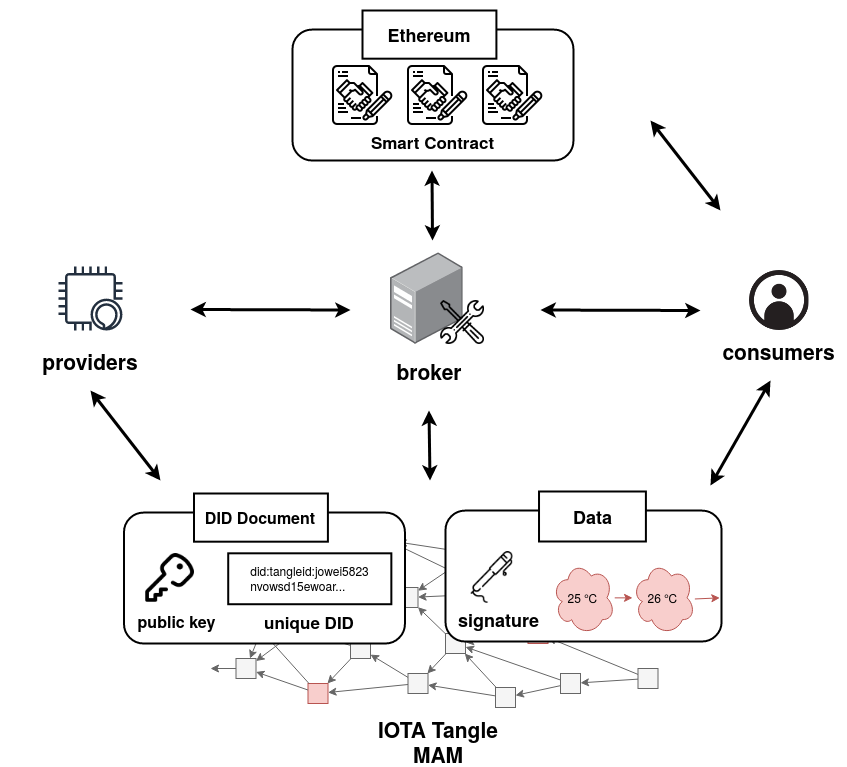
\includegraphics[width=5.in]{img/system_design}
    \caption{The system design of a decentralized data trading infrastructure which consists of data providers, consumers and brokers.}
    \label{fig:system_design}
\end{figure}

\end{spacing}

\clearpage
\setstretch{1.2}

% ------------------------------------------------
%                  Related Work
% ------------------------------------------------
\newpage
\phantomsection
\chapter{Related Work}
\label{section:relatedWork}
\pagestyle{plain}

\begin{spacing}{2.0}

\section{The Publish/subscribe Communication Models Over Blockchain}
The pub/sub service model consists of publishers, subscribers, and brokers, which has been proven\cite{pubSubAnalysis, pubSubAnalysis2} to be an efficient and flexible solution for a large number of diverse entities like IoT applications. A lot of work in the pub/sub system built on top of blockchain focused on the reliability, scalability, and the different security issues such as, encrypted data communication, privacy-preserving data subscription, and access control of the digital asset.

M. B. Abdullahi and G. Wang\cite{centralPubSub} presented a secure pub/sub data storage service in Wireless sensor networks (WSNs) which ensures several security issues. Each user has an identity for authentication, whereas subscribers' interests are encoded before matching to protect users' interests. Additionally, the proposed encryption scheme can prevent adversary to access published data if the sensor node is compromised. However, the access control and encryption keys of data are enforced by the network controllers (NCs) and CAs, which may be a potential security risk of the system, e.g., single-point failure. G. S. Ramachandran et al.\cite{trinity} pointed out the security risk of centralized brokers and applied DLTs to build a distributed pub/sub system that promotes the transparency of interactions of participants and the status of data. With the help of the Ethereum smart contract, users can perform data validation easily, and brokers can keep track of data status. But data is plaintext on blockchain, in which the privacy problem of sensitive data needs to be considered carefully.

In \cite{userCentricData}, the publisher runs a node in blockchain that preserves all the history data of the ledger, therefore, they can publish and manage data without any third-parties. The subscribers request publishers directly and ask them to save a cache space for interesting data. The main contribution of the system is to ensure data owners have full controls of produced data, but the data owners need to have well devices and environments to perform such functionalities and preserve data. Also, the rights for accessing digital assets are more compatible in the IoT scenarios instead of copying raw data. Secure Pub-Sub model\cite{SPS}, a brokerless pub/sub model, is proposed to eliminate the security risk of middleware in the model and to provide a reputation-based fairness payment strategy on blockchain. The privacy and data security are considered thoroughly with the encryption scheme, while the reputation system, the punishment rules against malicious acts of subscribers and publishers, payment, and data sharing are deployed on smart contracts that allow all operations are transparent. Yet, without brokers, providers and subscribers may need to reveal more sensitive information like IP address in order to match both sides. Another broker-less model in \cite{PrivacyPreservPubSub} protects the subscribers' privacy by encrypting users' interests with the light-weight PKEwET\cite{PKEwET}, which allows publishers to match the subscribers' interests in the ciphertext.

The previous works contribute to different aspects of building a reliable pub/sub system over blockchain. However, a few work propose an overall thinking of the pub/sub system, which ensures the privacy of players, preserves data securely and make data trackable, which is a vital consideration for IoT and mobile computing across organizations, and even stimulates data economics.

\section{Trusted IoT Trading Infrastructure}
Multiple infrastructures for trusted IoT data trading have been proposed. Paolo Missier et. al\cite{MindMyValue} presented an IoT brokered infrastructure based marketplace that enables trading with Ethereum smart contracts. The brokers are only responsible for data transmission in order to adapt flexible agreement between participants. Unlike the standard pub/sub model that matches publishers and subscribers that participants are unaware of each other. However, the data cubes (i.e., a tuple of information, such as provider, subscriber, and time period) are stored in a centralized Cassandra NoSQL database, which is guaranteed to be tamper-proof but the risk of single-point failure still exists.

A. Colman et al. \cite{TrustedMarketplaceWearable} discussed on trading the sensitive data among wearables. Several security issues are well discussed and solved with DLTs in the paper, the system consists of multiple components aiming for different responsibilities, such as data anonymizer eliminates keen information for privacy protection, access controller handles the key management and contract manager manages Ethereum smart contracts. While the trading processes are split into multiple servers, and the request/response communication model is applied, the scalability problem of the marketplace remains.

In the following researches, Masked Authenticated Messaging (MAM)\cite{MAM} is regarded as a secure data transmission layer and data storage built on top of DLT which provides access control, tamper-proof and authentication functionalities by tailoring messages to a channel. Jinzhi Lu et al.\cite{luDecentralizedDM} builds the data exchange system with MAM and IPFS\cite{IPFS}, a content-based addressing distributed storage system. Considering the limited transaction processing capability of DLT, the authors suggest to adopt IPFS to handle the encrypted large data sets, then add the encrypted IPFS link to MAM for further exchange. This research takes MAM as a data transmission layer only that focuses on secure data exchanging architecture design and security analysis, but the trading strategies are not studied yet. A similar infrastructure proposed by Zichichi et al.\cite{SocialGood} offered key and entry points management with MAM that minimizes the information which data producers need to hold. Also, Ethereum smart contract is used to maintain an authorized user list and to enable trading. However, the access control is examined by Authentication Service, the only client/server communication architecture, where the security issues and bottleneck of the system emerges from, and the details of trading and interactions between providers and consumers are not illustrated in this paper. Though taking IPFS as data storage instead of MAM is more efficient due to the current growth of underlying DLT, the chance of data losses and the efficiency of IPFS remain, which will be further discussed in Section.~\ref{section:distributed_storage}.

The researches below adopt MAM as data storage and a secure data transmission layer. The industrial data marketplace\cite{IOTAIdustryMarketplace} proposed by IOTA Foundation targets for IoT data streams trading. Service requesters call for proposals of interested data and accept/reject proposals from service providers. After a proposal is accepted, the requesters can access data streams stored via MAM and pay providers in IOTA tokens. This proposal matching and the trading procedure can be automated without any human guidance\cite{IOTAIdustryMarketplaceWithoutHuman}. Nevertheless, this trading model does not take into account the refund and unsubscribe mechanism, the service requesters still need to pay even if they want to unsubscribe or the data does not meet expectations.

O. Lamtzidis and J. Gialelis \cite{IOTASensorNode} proposed a distributed sensor node system to exchange data and establish a data monetization economy paradigm. The Back-End server helps sensor nodes to accelerate data uploads to MAM, manages keys and metadata of data streams, and evaluates data price according to its quality. Furthermore, the Back-End server operates a user-friendly interface of the marketplace and tackles all trading procedures. The heavy loading of Back-End server encounters the system scalability problem, single-point failure as well as malicious attacks which may damage the profits of all players. And the pricing strategy allows buyout but does not take subscribe/unsubscribe based diagrams into consideration. The decentralized data marketplace in \cite{DDMSmartCities} is fully decentralized without the existence of any intermediate server but data providers only, data providers attach, and trade data streams via MAM. With MAM, the data streams subscription is enabled, yet the conditions and details like refund and unsubscription are not discussed in this paper.
 
\section{Distributed Storage System}
\label{section:distributed_storage}
Decentralized storage systems allow users to store files in a distributed network that maintained by individual nodes around the world instead of a central service provider. Nevertheless, DLTs are often used as the backbone of these systems like data storage and also an incentive layer to encourage people to get involved in the network.

Filecoin \cite{FileCoin} in the Inter-Planetary File system (IPFS) is an incentive layer to incent nodes to provide storage. IPFS is a content-based addressing storage model in a peer-to-peer network, in which users can obtain the data with the unique hash value through the network. Furthermore, considering the data may lose in the network, IPFS provides \textbf{pin} command for users to store the contents locally that will not be removed. However, the IoT sensor devices have limited space which is not appropriate to preserve generated data. Also, users can have a hard time finding the contents quickly if data is not widely available, and the large amount of IPFS nodes and contents. Thus, several pinning services like Pinata provide multiple IPFS nodes around the world to pin users' contents and charge by the size and replicas of contents, and users can even join the dedicated network to speed up the retrieving process. Nevertheless, the efficiency problems still occur if the dedicated network grows larger.

Sia\cite{Sia} splits the uploaded file into multiple data segments encrypted with the owner's private key, then ciphertext is sent to the Sia nodes that rent the storage in Siacoin through smart contracts. Files are duplicated in multiple nodes to prevent data loss.

\end{spacing}

\clearpage
\setstretch{1.2}

% ------------------------------------------------
%               System Design Thinking
% ------------------------------------------------
\newpage
\phantomsection
\chapter{System Design Thinking}
\pagestyle{plain}

\begin{spacing}{2.0}
\label{section:design_thinking}
\section{Data Subscription-based Trading Platform Players}
There are three major roles, data providers, data consumers, and brokers which are similar to the pub/sub messaging model. But unlike the standard pub/sub model where brokers link the publishers and subscribers who are not aware of each other, in our proposed architecture, the brokers are only responsible for message delivery and essential verification processes. As shown in Fig.~\ref{fig:pub_sub_model}.

\begin{figure}[H]
    \centering
    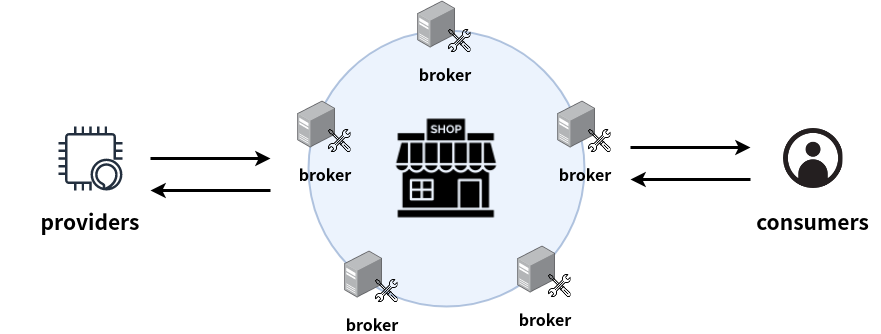
\includegraphics[width=4.5in]{img/pub_sub_model}
    \caption{The players in data subscription-based trading platform consists of data providers, data consumers and brokers.}
    \label{fig:pub_sub_model}
\end{figure}

\begin{itemize}
\item \textbf{Data Provider: }
Data providers are the ones that generate streaming data and set the data price based on the different types of data. Subscription fees can motivate data providers to maintain and improve the quality of data.
\item \textbf{Data Consumer: }
Data consumers are entities that are willing to buy data streams. As it is laborious to widely deploy devices to collect data from scratch and it is also difficult to find desired data sets, purchase is the fastest and efficient way to get the desired data sets.
\item \textbf{Broker: }
Brokers are responsible for building an agreement between data providers and consumers. Brokers are required to be online for providers and consumers, and they are incentivized by charging brokerage fees.
\end{itemize}

We adopt the brokered infrastructure for three reasons. Firstly, it inherits the benefits from the standard pub/sub model which is more efficient than the request/response model specifically in a large scale system. Furthermore, if either side is offline, the proceeding tasks have to stop and start over. With brokers, the unfinished work can be cached or accomplished. Second, a fully decentralized architecture has difficulties to brings data providers and consumers together, both of them need to reveal more sensitive information, such as IP address, in order to build the communication tunnel. The existence of brokers resolved the privacy issue, as brokers are the bridges that link data providers and consumers, participants can trade with minimum information like its identifier and public key. Third, a refund process needs a broker to host and supervise the procedures in order to protect the rights of participants, which will be further discussed in Section.~\ref{section:refund}.

\section{Choice of Data Storage}
Data storage is the trust basis of data trading platforms where the data assets are reserved. Streaming data unlike a fixed set of data that can be verified by the hash of the whole pack of data, it consists of continually granular records of each time slot. Therefore, the verification such as, data integrity and source identity is narrow down to a data point as well. In our proposed architecture, we adopt MAM as data storage to resolve the challenges of managing and verifying data streams. MAM is the second layer data communication protocol built on top of IOTA\cite{IOTAwhitepaper} network, the Tangle, a feeless cryptocurrency designed for IoT, which introduces properties like publishing, classifying and tracking authenticated message streams. Carrying these properties, MAM is also appropriate for building a self-sovereign identity system where the identity information such as public key, unique identifiers of services and metadata are stored. One can easily prove himself by sharing the identifier on MAM without any authority.

Currently, considering the efficiency of uploading large files, IPFS performs better than MAM (i.e., writing contents to IOTA network). However, IOTA network scales when more users and transactions join, and the MAM operations can be delegated to powerful proxy servers which will be illustrated in Section.~\ref{section:ta_endpoint}. Furthermore, adopting IPFS in IoT scenarios may meet the challenges of data loss and data retrieving efficiency.

In our work, MAM builds the trust of the platform while meeting the requirements of data trading which can be concluded below:

\begin{itemize}
    \item \textbf{Scalability}:
    \begin{itemize}
        \item Benefits from the underlying Tangle network, the system scales when more participants and more transactions join the network.
        \item For both data providers and consumers, MAM keeps the number of managed keys and data entry points as small as possible
    \end{itemize}    
    \item \textbf{Integrity}:
    \begin{itemize}
        \item Messages published to the Tangle are tamper-proof against malicious modifications.
        \item Messages are signed with the keys pre-generated under Merkle signature scheme\cite{MSS} (MSS) that both keys and messages can be verified by participants.
    \end{itemize}
    \item \textbf{Confidentiality}:
    \begin{itemize}
        \item The encrypted data are uploaded that only participants that have keys can decrypt.
        \item The authorized users can retrieve data streams since data is written on the Tangle which can be queried as long as the IOTA network is alive.
        \item MAM provides forward-secrecy. The entry points of future data can be derived, but it's impossible to trace back those in the past. This feature prevents adversaries from retrieving published history even if the key is revealed.
    \end{itemize}
\end{itemize}

MAM publishes authenticated streaming data to channel and endpoint as zero-value transactions to the Tangle and provides the ability to publish and fetch encrypted messages over the network along with data integrity and access control. The payload of a MAM message can be encrypted with an \textbf{encryption key} that restricts only authorized players can access contents, the ciphertext is then signed with \textbf{signature key} generated with MSS and attached to the Tangle. This approach allows users to validate the signatures without knowing the actual contents but ensuring the messages do come from the exact source. See Fig.~\ref{fig:channel_and_key} for illustration.

Using MAM as a data storage benefits from the scalability of the underlying IOTA network as well as the decentralized and fault-tolerant characteristics of distributed ledgers, which reduce the risks of centralized storage services. Furthermore, the rights of data access are traded instead of a copy of data in the trading platform, which eliminates the need for data consumers to have additional storage.

\begin{figure}
    \centering
    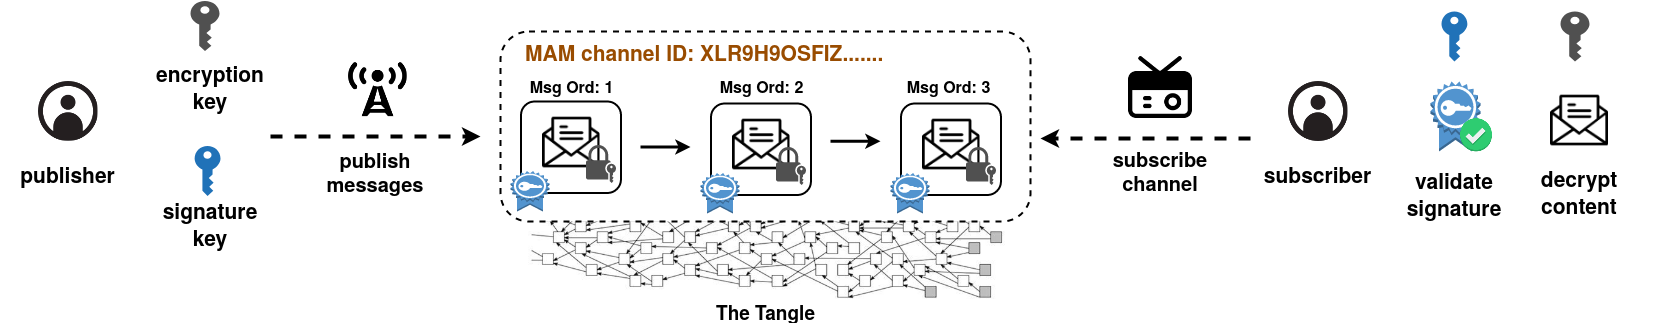
\includegraphics[width=6.5in]{img/channel_and_key}
    \caption{Within MAM channel, the message publisher has 2 types of key, an encryption key for encrypting contents and a signature key per message for digital signatures. Subscribers can validate the messages with signature keys and decrypt them with the encryption key.}
    \label{fig:channel_and_key}
\end{figure}
\clearpage

\section{Digital Identity}
The digital identity represents entities and holds the digital assets within the digital world, it is important to prove and show the identity to others during interactions. We select the decentralized identity model rather than a centralized one for the concerns in Table.\ref{tab:did}.

\begin{table}[h]
	\caption{The comparison of centralized and decentralized identity model}
	\label{tab:did}
	\begin{tabular}{|c|c|c|}
	\hline
		\textbf{Identity Model} & \textbf{Centralized} & \textbf{Decentralized} \\
		\hline
		Control & Enterprises control identities & Entities control their identities \\
		\hline
		Security & \makecell{Identity held in a centralized service \\ is a  honeypot for cyber attacks} & \makecell{Decentralized identity \\ limits data exposure} \\
		\hline
		Portability & \makecell{Identity is fragmented \\ across enterprises} & \makecell{Identity can be portable \\ across enterprises} \\
		\hline
	\end{tabular}
\end{table}

The centralized identity model may have the single-point failure in identifier management and security issues like data leakage. With sensitive information holding on certain authorities, the leakage caused by cyber-attacks or unscrupulous organizations trading user data damage the users' privacy. Furthermore, having a recognizable and portable identifier is important, otherwise, it is hard to cooperate fragmented identities of different data formats among institutions, and organizations may not approve identifiers of others. The decentralized identity model give back the controls of data to users that can resolve the aforementioned concerns in the centralized one.

In the decentralized identity model, every entity has a Decentralized Identifiers (DID\cite{DID} defined by W3C that contains identity information such as public key, unique identifiers of services and metadata. The digital footprints of entities are made up of Verifiable Credential (VC) added to their DIDs, issued by trusted issuers, such as schools and government departments. If a VC is verified via the issuer's public key, the message will be labeled as trusted. Fig.~\ref{fig:did_vc} shows the relationship of VC issuer, verifier and user.

\begin{figure}[h]
    \centering
    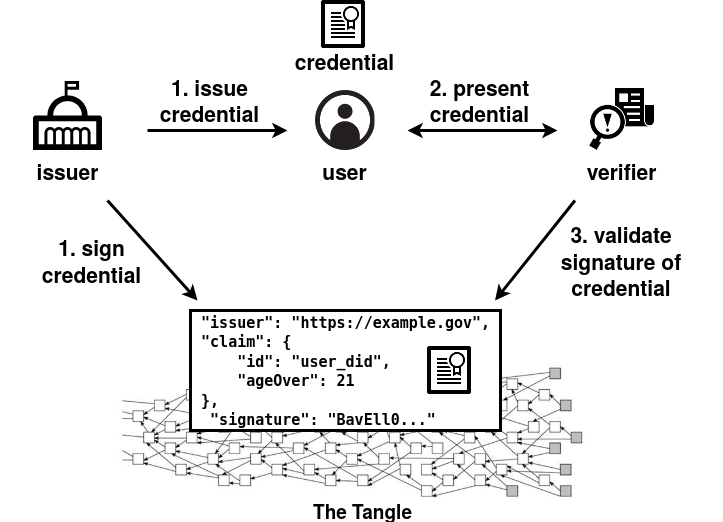
\includegraphics[width=4.5in]{img/DID_VC}
    \caption{The trusted issuer requests user's DID, then issues a VC with his/hers signature. The user can then present the VC to verifier for signature validation.}
    \label{fig:did_vc}
\end{figure}

In our architecture, a decentralized identity system TangleID\cite{TangleID} is used, which is built on top of MAM where change logs of DIDs are traceable. One can easily prove himself by sharing the identifier on MAM without any authority.

Through TangleID, entities get a public/private key pair, the location of the DID document, and the seed (i.e., the identifier of its owner in IOTA) that used to generate the DID document MAM channel. The public/private key pair can be used to exchange sensitive data and establish trust communication, where messages that are encrypted with a public key can only be decrypted with the private key owner. During data subscription process, the encryption keys of data products are encrypted with data consumers' public key on the DID document which ensures only the subscribed consumers are accessible. See Fig.~\ref{fig:TangleID}.

\begin{figure}[h]
    \centering
    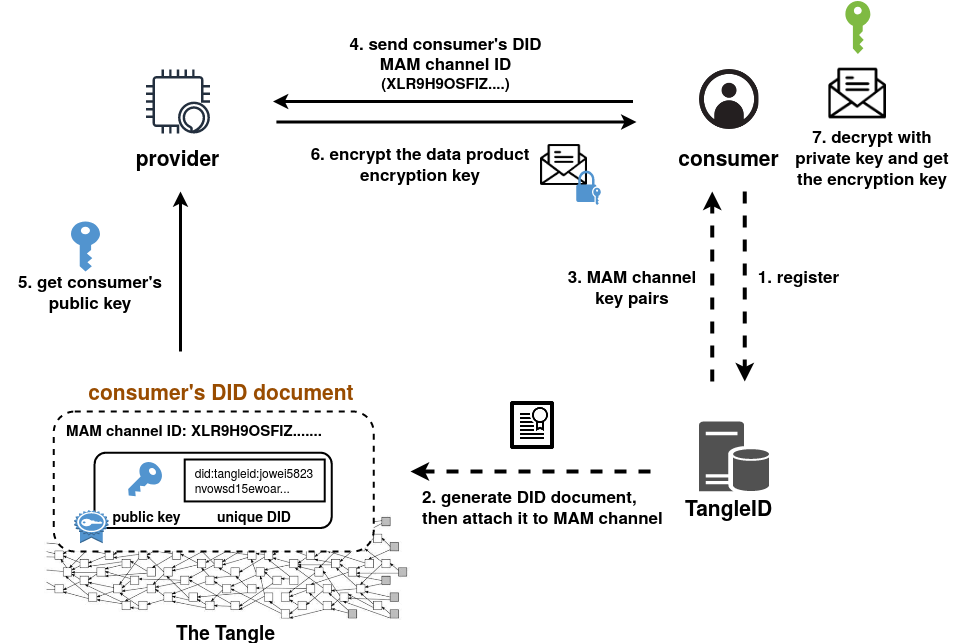
\includegraphics[width=5.5in]{img/TangleID}
    \caption{To participate in the data trading, players are required to have DID document issued by TangleID. The consumer first needs to send a registration request to TangleID to get the MAM channel ID of the DID document and a public/private key pair for authentication. When the trade establishes, the consumer sends the DID MAM channel ID to the provider in order to perform encryption key exchange. The data provider can then retrieve the consumer's public key and encrypt the content with it. After the consumer gets the encrypted message, he/she can decrypt the ciphertext with the private key and finally get the encryption key of data product.}
    \label{fig:TangleID}
\end{figure}
\clearpage

\section{Enable Automated Trading Process}
Ethereum is a cryptocurrency building on top of a public blockchain-based distributed ledger. It provides the smart contract, which is a protocol for formulating agreement on a blockchain that running on decentralized virtual machines. A smart contract can interact with other contracts, make decisions, store data, and transfer cryptocurrency. All the participants in Ethereum can verify and execute the contracts, and once the contract is triggered, it is uninterruptible and will be executed automatically without any third-parties.

With the functionalities of Ethereum smart contracts, a flexible and verifiable trading mechanism can be achieved. In our system, \textbf{Product Contract} is made for the product launching and subscribing. The information on data products such as the address of the data provider, subscription fee, brokerage fee, the threshold of consent votes of refunding, MAM channel/endpoint ID (the data entry point), time period, and the broker-verified encryption key are listed on Product Contract. Listing. \ref{lst:constructor} list the data fields of Product Contract, and Fig.~\ref{fig:smart_contract_mam} shows the relationship of Product Contract and MAM.

Furthermore, the participants can exchange encryption keys without any authorities via smart contracts. Though this design may cost extra transaction fees than exchanging key off-chain, it is considered a more secure strategy to protect the privacy of participants that only the DID document address and Ethereum addresses are revealed during the subscription process. Binding trading and data storage to smart contracts ensures consumers can always have access after payment, even if the key is lost, and providers can track and manage the authorized user list.

\begin{figure}[h]
    \centering
    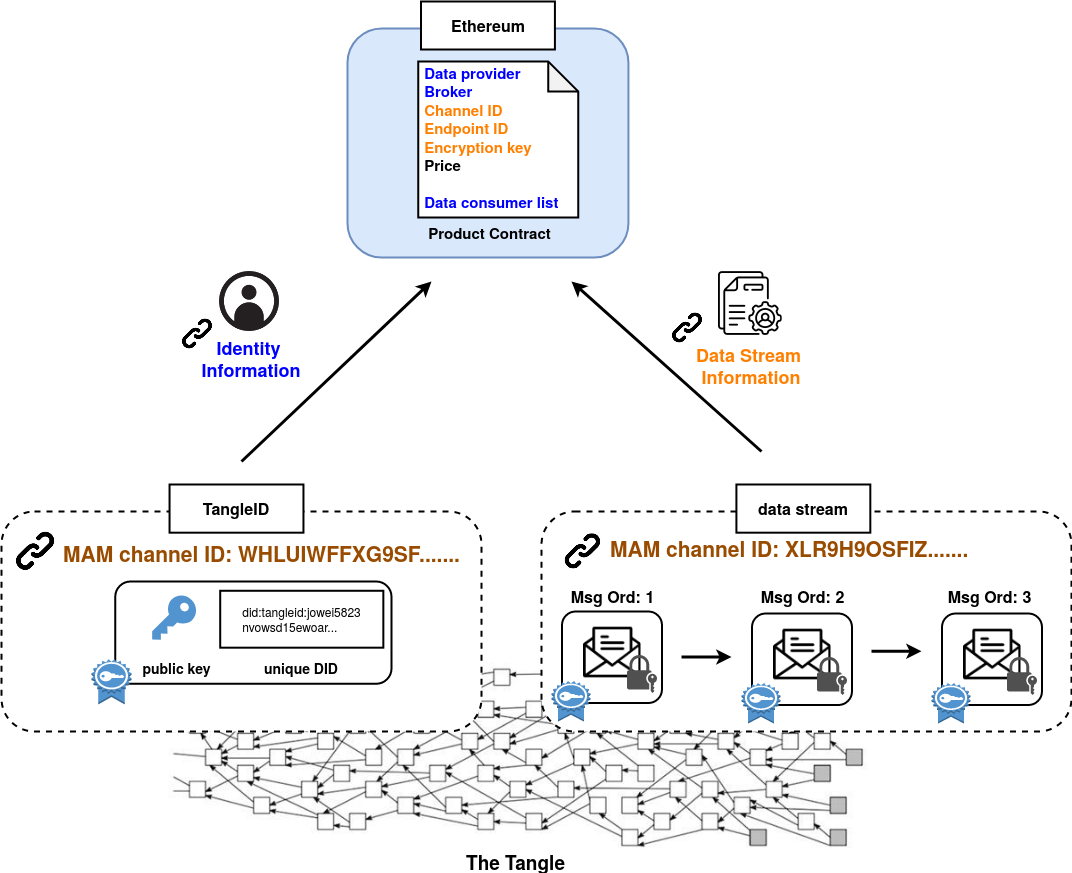
\includegraphics[width=5.5in]{img/smart_contract_mam}
    \caption{The information of identity and data streams are stored on the Tangle with MAM which is all recorded on Product Contracts. Participants can easily retrieve information via the Product Contract and proceed to trade. For signature validation check and further encryption key exchange, the MAM channel ID of participants' DID document are written down, presented in blue color. The orange color stands for the information of data products, which includes the data stream channel/endpoint ID.}
    \label{fig:smart_contract_mam}
\end{figure}
\clearpage

The transparency of smart contracts brings advantages for data providers and consumers. One of the advantages is that the trading states and progress are visible and verifiable which profits providers and consumers respectively. For data providers, with every detail opened, the consumer list functions like a reputation evaluation, the better the quality the more the consumers he/she has, which are also reputation references for data consumers. The enforcement of smart contracts also ensures the rights of participants that they fulfill the agreed contract under any circumstances.

\lstdefinestyle{solidity}{
	numbers=left,
    numbersep=1em,
	captionpos=b,
	tabsize=4,
	basicstyle=\linespread{0.9}\small
}
\lstset{style=solidity}
\begin{lstlisting}[caption={Product Contract data fields}, label={lst:constructor}, frame=single]
contract Product {
    address public broker;
    address public provider;
    bool isBrokerWithdraw;
    bool isProviderWithdraw;
    address[] consumers;
    
    struct Purchase {
        bool affirmativeVote;
        bool isConsumerWithdraw;
        bool isKeyAdded;
        bool isSubscribe;
        string encryptKey;
    }
    mapping(address => Purchase) public consumer2Purchase;
    
    uint public price;
    uint public totalAmount;
    uint public brokerage;
    uint public cancellation;
    uint public threshold;
    string public channelRoot;
    string public endPoint;
    uint public totalNumber;
    uint public uploadedNumber;
    uint public affirmativeVotes;
    string hashedKey;
    string certifiedKey;
    
    enum State {Launched, KeyCertified, Finished, Refunded}
    State public state;
}
\end{lstlisting}
\clearpage

\section{Enable Computation Tasks Delegation to Broker with Privacy}
To manage data products and to benefit from trading, data providers have to interact with MAM and Ethereum smart contract while doing its original tasks. However, the limited resources of low-level devices should be used in their jobs instead of handling all trading processes. Therefore, the operations of MAM and smart contracts are better to be delegated to brokers. The delegation should ensure the privacy of data providers, for instance, brokers are asked to attach messages to MAM and record encryption keys to smart contracts without knowing the contents. The encryption key upload procedure is illustrated in Section.~\ref{section:launch_data_product}.

As for MAM operations, the performance results in Section.\ref{section:mam_performance} show that operating MAM costs a lot of resources for the devices, therefore, we present an alternative solution for data providers to delegate these computing tasks to powerful proxy servers, Tangle-accelerator\cite{TA}, while ensuring the privacy. The details would be further illustrated in Section.\ref{section:ta_endpoint}.

\end{spacing}
\clearpage
\setstretch{1.2}

% ------------------------------------------------
%                 Masked Authenticated Messaging
% ------------------------------------------------
\newpage
\phantomsection
\chapter{Masked Authenticated Messaging}
\pagestyle{plain}

\begin{spacing}{2.0}
\label{section:MAM}
MAM enables broadcasting encrypted and authenticated data stream, referring as a channel, on the Tangle. The publisher publishes messages that are propagated through the network and can be accessed by the subscribers only. With MAM, the rights of data access are traded instead of a copy of data in the trading platform, which eliminates the need for data consumers to have additional storage.
Section.~\ref{section:mam_streams} to ~\ref{section:mam_features} explain the structure, fuctions and features of MAM proposed by IOTA Foundation, and our proposed MAM delegation mechanism is clarified in Section.~\ref{section:ta_endpoint}.

\section{The Message Streams}
\label{section:mam_streams}
A channel/endpoint is a stream of MAM transaction bundles, which consist of signature and the masked message payload. To publish a MAM message to a channel, MAM deploys MSS to sign the message payload to the channel, where $channel\ ID = root$ i.e., the MSS Merkle root. The Merkle tree is generated with \textbf{seed}, an identifier of its owner in the IOTA protocol, represents the ownership of all things associated with the user in the IOTA ecosystem. Furthermore, the structure of channel/endpoint implements forward linking, each address of a message can be derived from the previous one that other entities can fetch the next payload. This design also brings the advantage of forward secrecy, where no one has access to the data back from his/her entry point. Figure.~\ref{fig:mam_structure} shows the structure of the MAM channel/endpoint.

\begin{figure}[h]
    \centering
    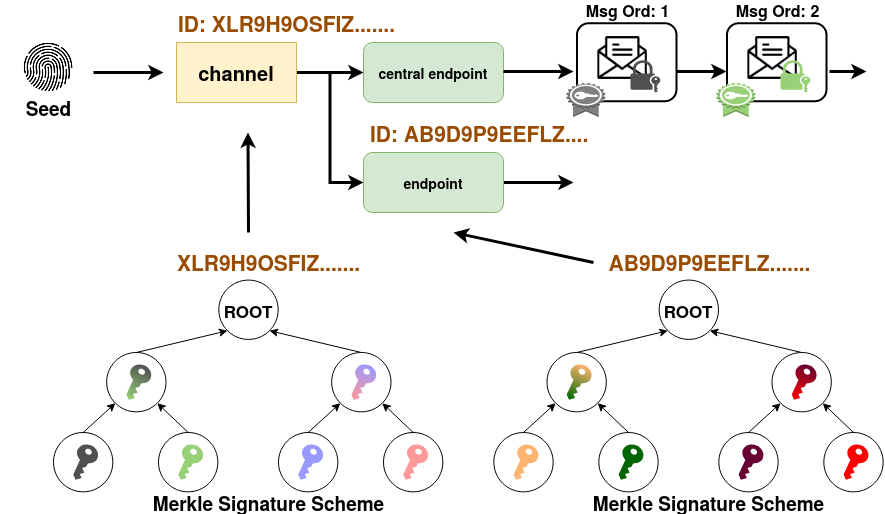
\includegraphics[width=5.5in]{img/mam_structure}
    \caption{With a seed, users can generate multiple channels, which can then generate multiple endpoints. The IDs of channel and endpoint are the roots of different Merkle trees in MSS. The "central endpoint" are endpoints that has ID, where $endpoint\ ID = channel\ ID$.}
    \label{fig:mam_structure}
\end{figure}
\clearpage

\section{Enable Access Control and Authentication}
\label{section:mam_functions}
The access control can be enabled via encryption with NTRU\cite{NTRU}, a quantum secure cryptosystem, or Pre-shared key (PSK), to prevent random users retrieving the data from channels. If the message payload is encrypted, subscribers are required for encryption keys to decode messages. The authentication in MAM includes two aspects: source and data. Source authentication ensures the message that originates from the claimed owner, and data authentication ensures the integrity of the data from the sender. These are achieved through the MSS and One-way hash functions by validating the signature added in the signature section of the MAM bundle. However, the size of Merkle Hash Trees, that is, the size of a channel/endpoint should be determined at the start. Thus, data providers need to first decide how to distribute data products into MAM channels/endpoints before uploading data.

\section{The Advantages of Adopting MAM in Subscription-based Data Trading Infrastructure}
\label{section:mam_features}
%scalability
\subsection{A Scalable Keys and Data Entry Points Management}
The importance of scalable key and data entry points management increases over time. In MAM, with an entry point (i.e., the address of transaction) and the encryption key, one can derive the following addresses of the transaction and retrieve data. To manage a data stream, the owner only needs to preserve 1 entry point and 1 encryption key in MAM, but $N$ entry points and 1 encryption key in other distributed storages.
\clearpage

%classify
\subsection{Data Streams Classification and Traceability}
The channel and endpoint structures enable users to be able to easily categorized data streams with respect to different types and usages. For instance, sensor devices like AirBox\cite{LASS}, collect environmental data, can split the statistics like PM 2.5 and humidity by time period into separate channels, which is useful for data providers to organize records and to pack into different data products. As for data traceability, users can easily track the footprints of data change logs as well as checking the validity of modifications with the signature.

\section{Delegate MAM Operations to Tangle-accelerator}
\label{section:ta_endpoint}
MAM builds a secure and authenticated communication protocol on top of multiple cryptosystems, which low-level devices need to spend a lot of resources to apply it, and they may not even support built-in libraries in the regular operating systems. To overcome these concerns, we propose another approach that allows data providers to delegate the MAM operations to Tangle-accelerators, proxy servers with high computation power, which can accelerate the interactions with Tangle while ensuring the privacy of data providers. Fig.~ \ref{fig:ta_struct} shows the structure of Tangle-accelerator, and Fig.~\ref{fig:delegation} shows how data providers can adopt MAM.
\clearpage

\begin{figure}[t]
    \centering
    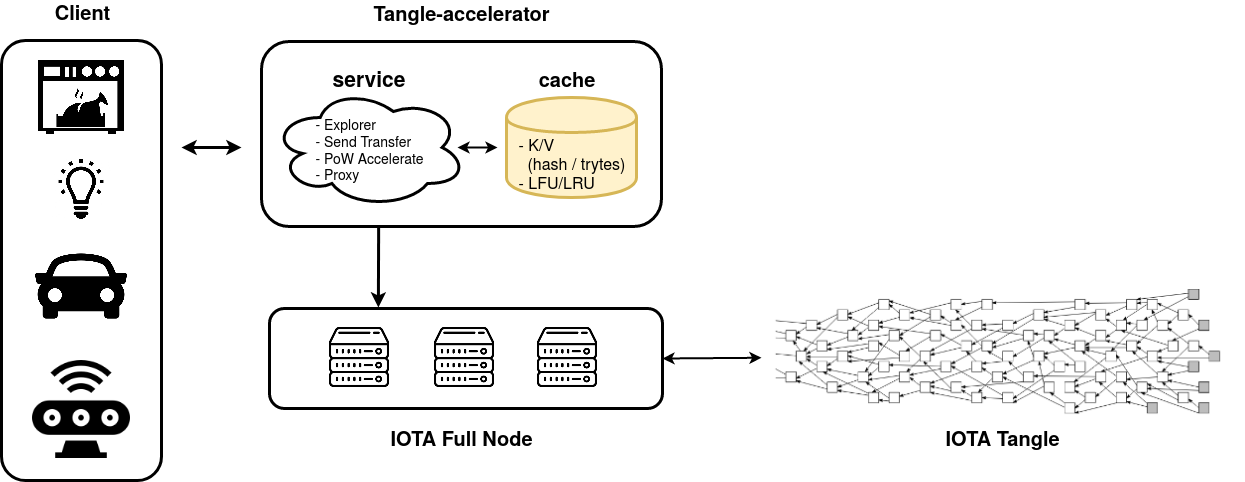
\includegraphics[width=5.5in]{img/ta_structure}
    \caption{Tangle-accelerator distributes IOTA API requests to idle IOTA nodes (i.e., full nodes) and provides Proof-of-Work acceleration. It can also cache the requests/responses in a key-value store to shorten response time, and automatically resend requests if failed. Tangle-accelerators also form a firewall for full nodes, which don't need to reveal the IP address to public and reduce the risks of being attacks.}
    \label{fig:ta_struct}
\end{figure}

\begin{figure}[b]
    \centering
    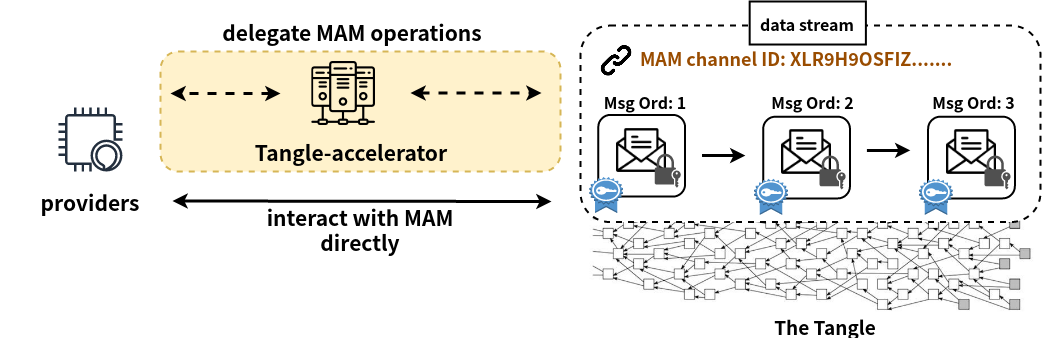
\includegraphics[width=\linewidth]{img/delegation}
    \caption{Data providers can use MAM in 2 ways: the provider performs MAM operations locally, and the provider delegates MAM operations to Tangle-accelerator.}
    \label{fig:delegation}
\end{figure}
\clearpage

\subsection{Communication Protocol}
In the following sections, we refer to the low-level devices as \textbf{endpoint}s. MQTT\cite{MQTT} is chosen as the communication protocol, which requires fewer TCP packets and less traffic. The topic-based pub/sub pattern and lightweight packet that MQTT adopts would undoubtedly play an important role in endpoints with limited bandwidth. The pub/sub model decouples publishers and subscribers in many ways:

\begin{itemize}
    \item Space decoupling: Both publishers and subscribers don't need to know each other.
    \item Time decoupling: Publishers and subscribers do not need to be active at the same time.
    \item Synchronization decoupling: Operations are decoupled from the publishers and subscribers. The publishers do not need to be alive until the response arrives. Messages from the publisher can be served as send-and-forget fashion.
\end{itemize}

\subsection{End-to-End-Encryption}
Introducing a proxy server to process all the cryptographic operations causes the proxy server or the middle man can easily tamper the message. To avoid such malicious operations during transmission, we introduce another lightweight end-to-end-encryption (E2EE) upon MAM protocol. The plaintext will be encrypted with this lightweight end-to-end-encryption. The E2EE process ensures only authorized subscribers can read the messages published on MAM.

%pic
\begin{figure}[h]
    \centering
    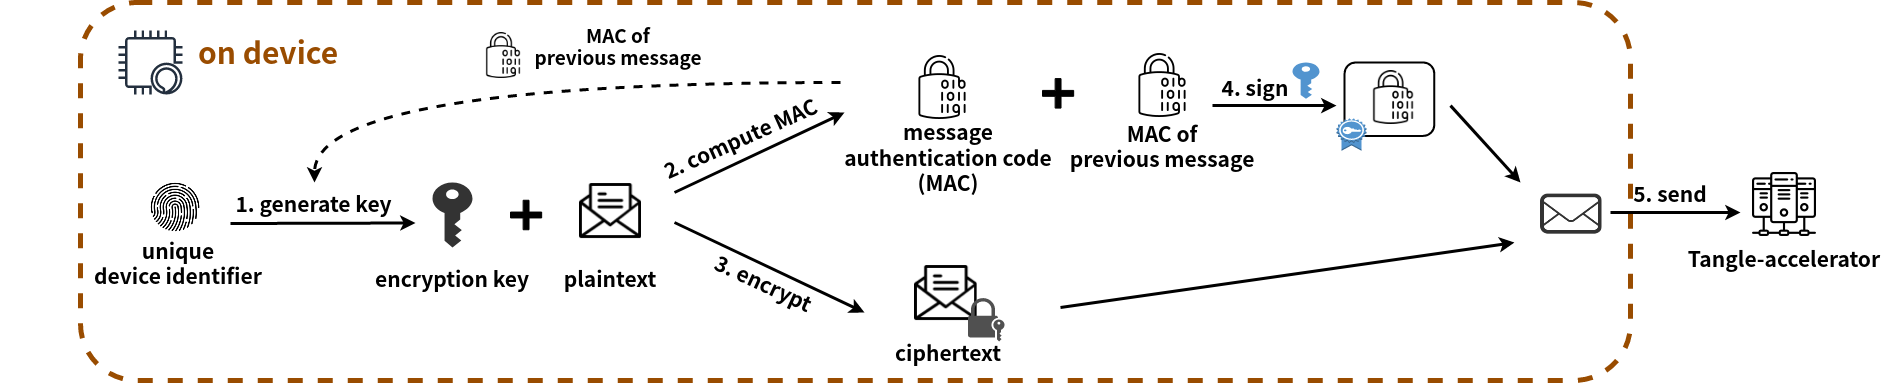
\includegraphics[width=6.5in]{img/MAM_E2EE}
    \caption{The process of E2EE.}
    \label{fig:MAM_E2EE}
\end{figure}

In the Fig.~\ref{fig:MAM_E2EE}, we illustrate each step of the presented E2EE process. The details of steps are addressed below:

\begin{enumerate}
    \item Generate symmetric keys with the unique device identifier and Message Authentication Code (MAC) of the previous message. If the message is the first one, then sharing secret initialization information would serve as the MAC of the previous message. Key Derivation Function (KDF) is used to generate the symmetric keys.
    \item Compute the MAC of the current message with the Hash-based Message Authentication Code(HMAC). Both plaintext and the symmetric key would be given as parameters in HMAC.
    \item Apply the generated symmetric key to encrypt the plaintext.
    \item Concatenate the MAC of the current message and the MAC of the previous message, then the result will be signed with a digital signature algorithm.
    \item Send the ciphertext along with the signed MAC.
\end{enumerate}

\begin{table}[htbp]
    \caption{AES256 Encryption Performance Numbers}
    \label{tab:AES_NI}
    \begin{center}
        \begin{tabular}{ |c||c|c|c|  }
            %\hline
            %\multicolumn{4}{|c|}{} \\
            \hline
            Size& \makecell{NON AES-NI \\ (msecs)} & \makecell{AES-NI \\ (msecs)} & \makecell{Encryption \\ Acceleration (\%)} \\
            \hline
            50 MB  & 1026  & 563   & 45.13 \\
            100 MB & 2036  & 1297  & 36.30 \\
            200 MB & 4282  & 2984  & 30.31 \\
            512 MB & 10754 & 6401  & 40.48 \\
            1 GB   & 23976 & 15721 & 34.43 \\
            \hline
        \end{tabular}
    \end{center}
\end{table}

The E2EE protocol presented in this thesis combines a series of different cryptographic procedures. Each of them can be chosen on the basis of the working hardware and scenario by developers. On certain devices, hardware acceleration would be supported. With hardware-acceleration, the elapsed time could be dropped a step more. For example, applying AES-NI can accelerate AES operations around 40\% on Intel devices.\cite{AES-NI-Acceleration} According to Intel, Table~\ref{tab:AES_NI} shows the performance of Encryption of AES256 with and without hardware acceleration.

\subsection{Register with Tangle-accelerator}
Users with channel seed can acquire channel chain ownership. Seed is generated by unique hardware information on the edge device, so it should be transmitted to Tangle-accelerator to publish messages on the MAM channel chain. Once the Tangle-accelerator receives the Seed from the edge device, it would return a unique user identifier that can be mapped to corresponding Seed when edge devices send requests. Asymmetric encryption is utilizing during the process of exchanging seed. The digital signature should be performed at the same time to ensure data integrity. Once the seed has been successfully exchanged, the edge device is successfully registered on the specific Tangle-accelerator. Thus, the seed will not be exposed during communication in further usages.

\subsection{Issues in End-to-End-Encryption}
E2EE helps a lot with low-level edge devices utilizing blockchain service. It dramatically reduces the execution time of encryption. However, we meet two challenges in the E2EE process:

\subsubsection{Time to Read Message}
It is linear time to decrypt messages instead of constant time. Nevertheless, there is one way to speed up the message decryption process. A subscriber can fetch multiple MAM messages with one API call, then the subscriber can decrypt the ciphertext at the local side. This procedure can reduce the time spending on internet communication.

\subsubsection{Spam on Message Channel Chain}
Tampering the messages which have conducted E2EE would be a challenging mission. However, spamming would be the critical issue participants may meet under this architecture. It is risky for an edge device connects to a Tangle-accelerator which is operated by unknown third-party. Sharing Channel Chain ownership with an unknown third-party would allow them to spam on the MAM Channel Chain. Spam would cause subscribers wasting plenty of time on decrypting useless messages. Since Tangle-accelerator can be easily hosted on regular personal computers, the actual device holders can set up an instance to prevent edge devices from such attack.

\end{spacing}
\clearpage
\setstretch{1.2}

% ------------------------------------------------
%  Decentralized Subscription-based Data Trading Case Study
% ------------------------------------------------
\newpage
\phantomsection
\chapter{Decentralized Subscription-based Data Trading Models}
\pagestyle{plain}

\begin{spacing}{2.0}
\label{section:trading_model}
In this chapter, we illustrate how participants can join the data subscription platform, start subscribing, cancel subscription, and request refund.

\section{Prerequisite}
All participants are required to register on TangleID to get a DID document and a  public/private key pair for sensitive contents exchange and authentication. An Ethereum account is also needed to interact with smart contracts and transfer Ethereum tokens.

\section{Launch Data Products}
\label{section:launch_data_product}
To launch a data product, data providers need to create a MAM channel/endpoint for data streams and a Product Contract. For those resource-constraint IoT devices, the MAM related operations can be delegated to Tangle-accelerator, as mentioned in Section.~\ref{section:ta_endpoint}. And brokers are responsible for Product Contract creation.

The details of data products, such as data price, MAM channel/endpoint ID, and the length of data stream are listed on the Product Contract. As regard to the encryption key of data product, data provider computes the digest of sensitive contents with a hash function, and sends the digest as well as the signature to a  broker. The broker can first verify the signature from data provider with the public key on the DID document. If it's valid, then the broker uploads the key; otherwise, the process will be aborted. Note that the broker needs to sign the encrypted encryption key he/she receives proving that it is uploaded by the responsible broker. This procedure allows data consumers to check whether the encryption key is uploaded by the committed data provider and broker before subscription. Furthermore, the encryption key can only be uploaded/updated under two circumstances: 1.) the new product launches. 2.) a data consumer unsubscribe to the product. Finally, the data product is launched and data providers can start uploading data. Fig.~\ref{fig:key_upload} demonstrates the key uploading process to the Product Contract via a broker. The product launching workflow is shown in Fig.~\ref{fig:launching_product} and Listing.~\ref{lst:key_certification} lists the Solidity codes of the key certification process.
\clearpage

\begin{figure}[t]
    \centering
    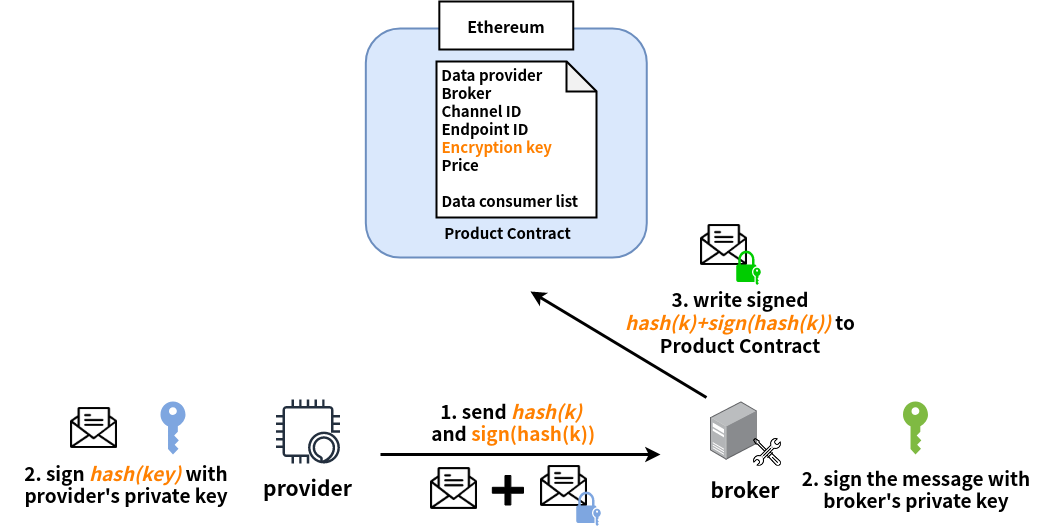
\includegraphics[width=5.5in]{img/key_upload}
    \caption{To add encryption key to Product Contract, the data provider sends the digest of the encryption key and the one that signed with his/her private key. After the broker receive the request, he/she performs digital signature as well to prove the encryption key is uploaded by the responsible broker, then writes the result to the Product Contract.}
    \label{fig:key_upload}
\end{figure}

\begin{figure}[b]
    \centering
    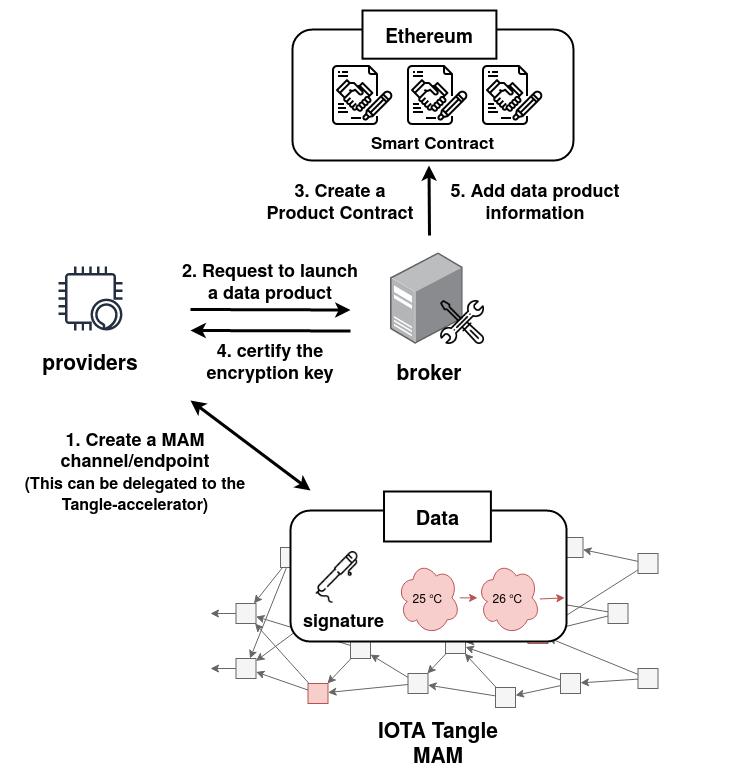
\includegraphics[width=4.5in]{img/launching_product}
    \caption{The process of launching a product.}
    \label{fig:launching_product}
\end{figure}
\clearpage

\lstset{style=solidity}
\begin{lstlisting}[caption={Functions of hased key update and certified key update}, label={lst:key_certification}, frame=single]
    function addHashedKey(
        string memory _hashedKey
    ) public {
        require(
            msg.sender == provider,
            "Only provider can add hashed key."
        );
        require(
            state == State.Launched,
            "One key has been certified."
        );
        hashedKey = hashedKey;
        emit newHashedKey(hashedKey);
    }

    function addCertifiedKey(
        string memory _certifiedKey
    ) public {
        require(
            msg.sender == broker,
            "Only broker can add certifiedKey."
        );
        require(
            state == State.Launched,
            "One key has been certified."
        );
        certifiedKey = _certifiedKey;
        state = State.KeyCertified;
        emit newCertifiedKey(certifiedKey);
    }
\end{lstlisting}
\clearpage

\section{Subscribe to a Data Product}
Data consumers pay subscription fees to the Product Contract of desired data products, and data providers give the encryption key of data stream instead of the files to consumers. The MAM channel/endpoint encryption key is encrypted with the public key of data consumer by the data provider and written on the Product Contract, which ensures only data consumers can decode it via Product Contract.

Transferring the encryption key on smart contracts instead of off-chain not only ensures the consistency of the encryption key but also prevents frauds from malicious participants, and the exchange process is transparent to the public. Furthermore, with the help of brokers and smart contracts, both data providers and consumers do not need to be online at the same time to proceed with the trading process. The key sending process is shown in Fig.~\ref{fig:key_exchange} and Listing.~\ref{lst:key_exchange}. The subscription fee is transferred from the Product Contract to data providers when the committed data is available on MAM.

\begin{figure}[H]
    \centering
    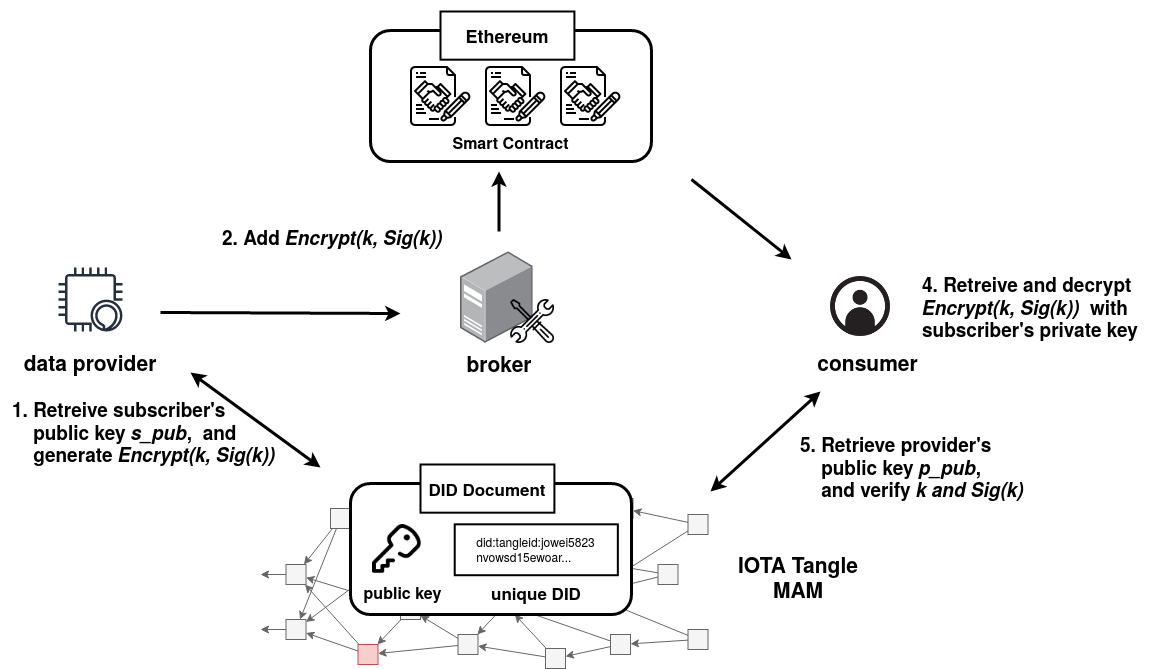
\includegraphics[width=5.5in]{img/key_exchange}
    \caption{Encryption key exchange process.}
    \label{fig:key_exchange}
\end{figure}
\clearpage

\lstset{style=solidity}
\begin{lstlisting}[caption={Add encryption key to data consumers}, label={lst:key_exchange}, frame=single]
function addEncryptKey(
    address _consumer,
    string memory _encryptKey
) public {
    require(
        msg.sender == provider,
        "Only provider can add the encrypted key."
    );
    require(
        consumer2Purchase[_consumer].isKeyAdded == false,
        "Encryption key has been added."
    );
    consumer2Purchase[_consumer].encryptKey = _encryptKey;
    consumer2Purchase[_consumer].isKeyAdded = true;
    emit newEncryptKey(_consumer, _encryptKey);
}
\end{lstlisting}

\section{Unsubscribe to a Data Product}
Data consumers can unsubscribe to data products when they're not interested anymore. Product Contract marks the consumer as not subscribing, corresponding to the parameter $isSubscribe$ in $Product$ structure since the delete function in Solidity does not remove the actual element but resetting it to default value. When data consumers trigger the unsubscribe event, a withdraw function is executed to pay a subscription fee to providers and return the rest of the fee back to consumers. The amount of payment distributed to different players is defined in formula~\ref{equation:unsubscribe_provider}, \ref{equation:unsubscribe_broker}, \ref{equation:unsubscribe_consumer}. $i$ is the number of data when unsubscription request is launched, $price$  is the subscription price, $M$ is the number of expected data samples, $F_{b}$ (\%) is the brokerage fee which is expressed as a percentage, $F_{t}$ is the transaction fee of the smart contract, and $F_{cancel}$ is the cancellation fee charged for unsubscription.

In SaaS, the cancellation fee is a way to make sure the service providers are protected. It is commonly used in pre-paid subscription-based services that allows service providers to charge cancellation fee if subscribers drop out at the early stage. However, asking the cancellation fee arbitrarily may cause an unfair contract which leads to the legal issue that should be carefully studied.

Also, data providers will change the encryption key of the data product to prevent unsubscribers access to the rest of the data. The new key should be updated to the remaining subscribers in the $consumer2Purchase$ list in the Product Contract. Fig.~\ref{fig:unsubscribe} shows the unsubscription flow.

\begin{equation}
\label{equation:unsubscribe_provider}
    F_{DataProvider}(i) = price \frac{i-1}{M} (1-F_{b}+F_{cancel}) -F_{t}
\end{equation}

\begin{equation}
\label{equation:unsubscribe_broker}
    F_{Broker}(i) = price \frac{i-1}{M} F_{b} -F_{t}
\end{equation}

\begin{equation}
\label{equation:unsubscribe_consumer}
    F_{Consumer}(i) = price (1-\frac{i-1}{M})(1 -F_{cancel}) -F_{t}
\end{equation}

\begin{figure}[h]
    \centering
    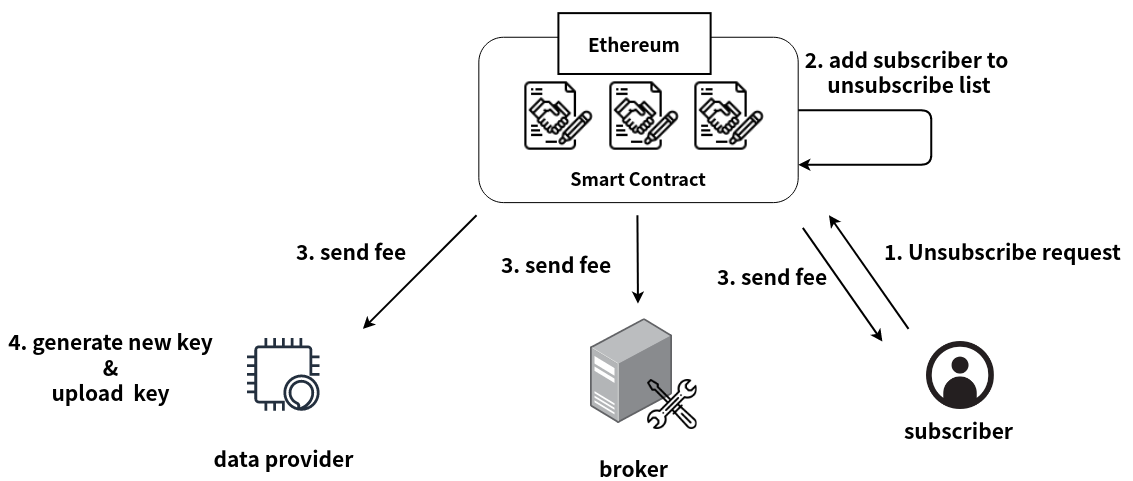
\includegraphics[width=5.5in]{img/unsubscribe}
    \caption{Once a data consumer launch a unsubscription procedure, he/she is marked as not subscribing and the Product Contract will distribute the funds to provider, broker and consumers respectively. Then, the data provider will generate a new encryption key and upload it for every remaining subscribers.}
    \label{fig:unsubscribe}
\end{figure}
\clearpage

\section{Launch a Refund}
\label{section:refund}
Data subscription is a high risk in which data provider may not upload data as the agreement after receiving the subscription fee. Therefore, in our proposed architecture, data consumers can trigger a refund procedure by sending a transaction on Ethereum if the data is not available or defective. When the refund procedure is launched, all consumers vote to decide whether the refund is established. See Fig.~\ref{fig:refund}. Once the ratio of consent votes of refunding is higher than a threshold, the subscription fee is proportionally transferred to the data provider, broker and every consumer as following, where $N$ is the number of consumers in this contract:


\begin{equation}
    F_{DataProvider}(i) = Nprice \frac{i-1}{M} (1-F_{b}) -F_{t}
\end{equation}

\begin{equation}
    F_{Broker}(i) = Nprice \frac{i-1}{M} F_{b} -F_{t}
\end{equation}

\begin{equation}
    F_{Consumer}(i) = price (1-\frac{i-1}{M}) -F_{t}
\end{equation}

\begin{figure}[h]
    \centering
    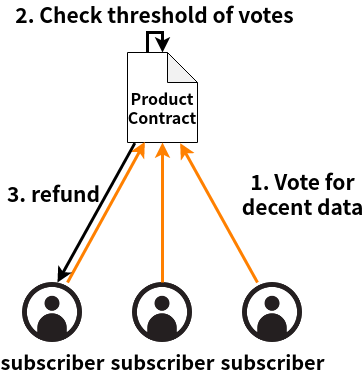
\includegraphics[width=2.5in]{img/refund}
    \caption{Once a data consumer launch a refund vote, all consumers start voting to decide whether they want a refund. Finally, the establishment of refund is determined by Product Contract after checking the number of votes is larger than a threshold or not.}
    \label{fig:refund}
\end{figure}

However, refund conditions are complicated in subscription services in the real world, participants can launch a refund in following conditions: First, as proposed methods above, consumers launch a refund vote when the data provider does not upload data as expected after receiving the subscription fee. Nevertheless, multiple issues still need to be investigated such as, consumers can only initiate a refund after getting the data or in a certain time period, the broker should host and set a vote timeline to count the votes, and handling the condition that not enough consumers join the vote need to be considered carefully. Second, brokers operate the subscription platform by earning brokerage fee, which is a deal between brokers and providers. If they can not reach a consensus of the brokerage fee during the subscription period, brokers can launch a refund and refuse to handle the product. Third, the refund could launch by providers when they fail to maintain products as committed.

\end{spacing}

\clearpage
\setstretch{1.2}

% ------------------------------------------------
%                   Evaluation
% ------------------------------------------------
\newpage
\phantomsection
\chapter{Evaluation}
\pagestyle{plain}

\begin{spacing}{2.0}
\label{section:evaluation}
We evaluate the cost of operating the subscription-based data trading infrastructure in two aspects: 1) Evaluate the cost of adopting MAM on devices, since it is the most commonly used component to data provider. 2) Evaluate the minimum cost for participants to sustain or subscribe to a data product via Product Contract.

\section{MAM Performance Evaluation}
\label{section:mam_performance}
It is worth making a claim that all participants in the data subscription platform do not need to hold an IOTA full node which maintains the transaction history and exchanges information of the Tangle. Each role is only required to run client libraries and communicate with IOTA full nodes to interact with the Tangle. Therefore, in the following evaluations, all devices run with client library only.

MAM is a secure and validatable data storage of the proposed architecture. And publishing data to MAM is the primary key to resolve all the difficulties discussed in previous sections. The interactions between data providers and MAM can be frequent. Data providers can either upload data in a short time interval or maintain multiple MAM channels or endpoints at the same time, hence the operation of MAM is one of the potential bottlenecks in the data subscription platform.

In this section, time measurement is evaluated in two MAM operations: channel/endpoint creation and data attachment to endpoints. To perform the evaluation assessment, a personal computer (PC, 3.2GHz 64-bit 6-core i7-8700 with 16GB DDR4 RAM) and a Raspberry Pi 3 Model B (1.2 GHz 64-bit quad-core ARM Cortex-A53 with 1GB LPDDR2 RAM) have been used to run MAM.

\subsection{Channel / Endpoint Creation}
The length of a channel or endpoint is $2^{height}-1$ where \textit{height} is the height of Merkle Hash Tree in a Merkle signature scheme (MSS), and the "$-1$" is for announcing the ID of next channel or endpoint. A channel with height $n$ can create $2^n-1$ endpoints, and an endpoint with height $m$ can attach $2^m-1$ messages, therefore the capacity of a channel is $2^{nm}-2^n-2^m+1$ messages in total. The greater the \textit{height} of MSS, the longer the channel/endpoint, however the higher the computational power required. In this task, both channel and endpoint creation are tested and the \textit{height} is set from 1 to 7 which is quite enough for data providers to upload data. The results are shown in Table \ref{tab:channel_create} and Table \ref{tab:endpoint_create}. The time duration for each \textit{height} is the average time of running 100 rounds.

\begin{table}[htbp]
	\caption{Time measurement of channel creation}
	\label{tab:channel_create}
	\begin{center}
	\begin{tabular}{|c|c|c|}
	\hline
		\textbf{height of MSS} & \textbf{PC (sec)} & \textbf{Raspberry Pi 3 (sec)} \\ 
		\hline
		1 & 0.26183 & 2.908702 \\ 
		2 & 0.524076 & 5.805524 \\ 
		3 & 1.045942 & 11.555660 \\ 
		4 & 2.092989 & 23.178036 \\ 
		5 & 4.19515 & 46.164079\\ 
		6 & 8.361586 & 92.320173\\ 
		7 & 16.651607 & 185.292243\\
		\hline
	\end{tabular}
	\end{center}
\end{table}

\begin{table}[htbp]
	\caption{Time measurement of endpoint creation}
	\label{tab:endpoint_create}
	\begin{center}
	\begin{tabular}{|c|c|c|}
	\hline
		\textbf{height of MSS} & \textbf{PC (sec)} & \textbf{Raspberry Pi 3 (sec)} \\ 
		\hline
		1 & 0.256425 & 2.887064 \\ 
		2 & 0.505679 & 5.767912 \\ 
		3 & 0.999524 & 11.550455 \\ 
		4 & 1.994017 & 23.260508 \\ 
		5 & 3.965007 & 46.748366 \\ 
		6 & 7.918925 & 93.182975 \\ 
		7 & 16.561419 & 186.064562 \\
		\hline
	\end{tabular}
	\end{center}
\end{table}

The results of Table \ref{tab:channel_create} and Table \ref{tab:endpoint_create} are plotted in Fig.~\ref{fig:mam_create}. Since the creation of channel and endpoint are MSS calculations, the curves of the same hardware are nearly identical. On the other hand, the performance of Raspberry Pi 3 is acceptable when \textit{height} is smaller than 4, but time grows rapidly when \textit{height} is 5 or above. And the performance of PC remains acceptable even \textit{height} gets to 7. The results indicate that MAM channel/endpoint creation is a laborious job for a Raspberry Pi 3 when data providers need a longer channel/endpoint, which is one of the reason that MAM operations should be forwarded to the Tangle-accelerator.

\begin{figure}[h]
    \centering
    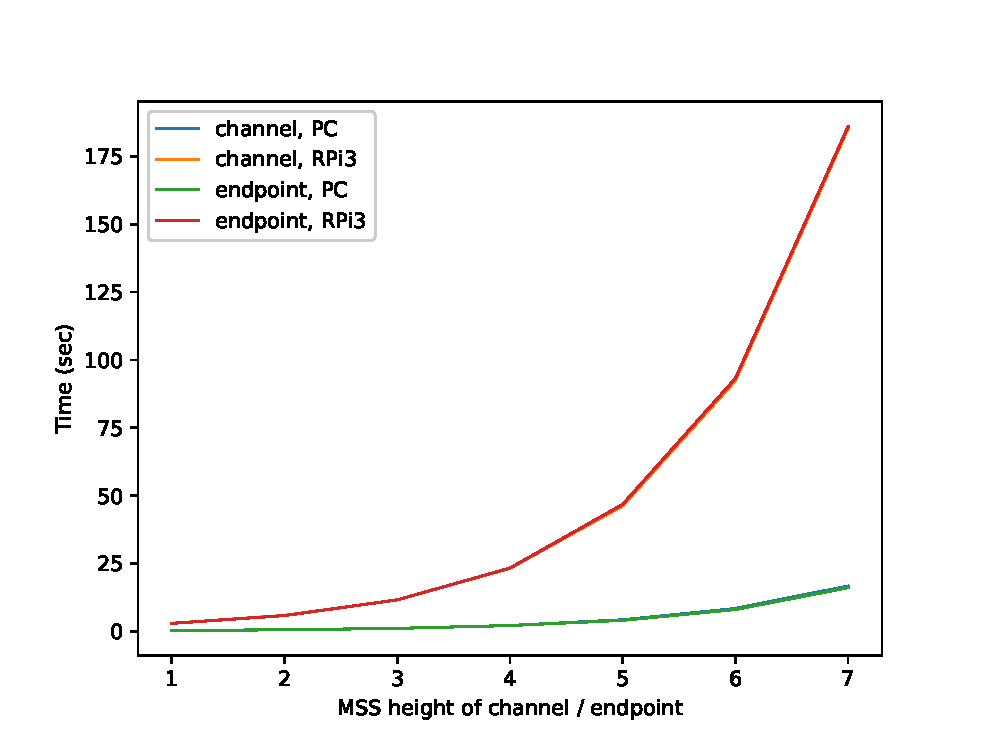
\includegraphics[width=5.in]{img/mam_create}
    \caption{Time cost of MAM creation.}
    \label{fig:mam_create}
\end{figure}

\subsection{Messages Publishment}
Publishing a message to MAM is attaching a zero-value transaction to the Tangle which requires two processes:
\begin{itemize}
    \item    Tips selection: In the IOTA protocol, a new-coming transaction needs to pick up 2 existed transactions called tips to reference and verify. The tips are provided by IOTA full nodes.
    \item    Proof-of-Work (PoW): An algorithm that prevents Denial of Service and spam attacks on a network. A computationally hard puzzle to solve, but easy to verify.
\end{itemize}

Tips selection requires a stable network connection to wait for the response from IOTA full nodes, and PoW requires enough computation resources to perform. Fig.~\ref{fig:mam_send} shows the probability distribution function of publishing a message to MAM endpoint. The time of Raspberry Pi 3 distributed widely since the randomness of PoW has a huge impact while all the tests on PC remain in an acceptable range.

\begin{figure}[H]
    \centering
    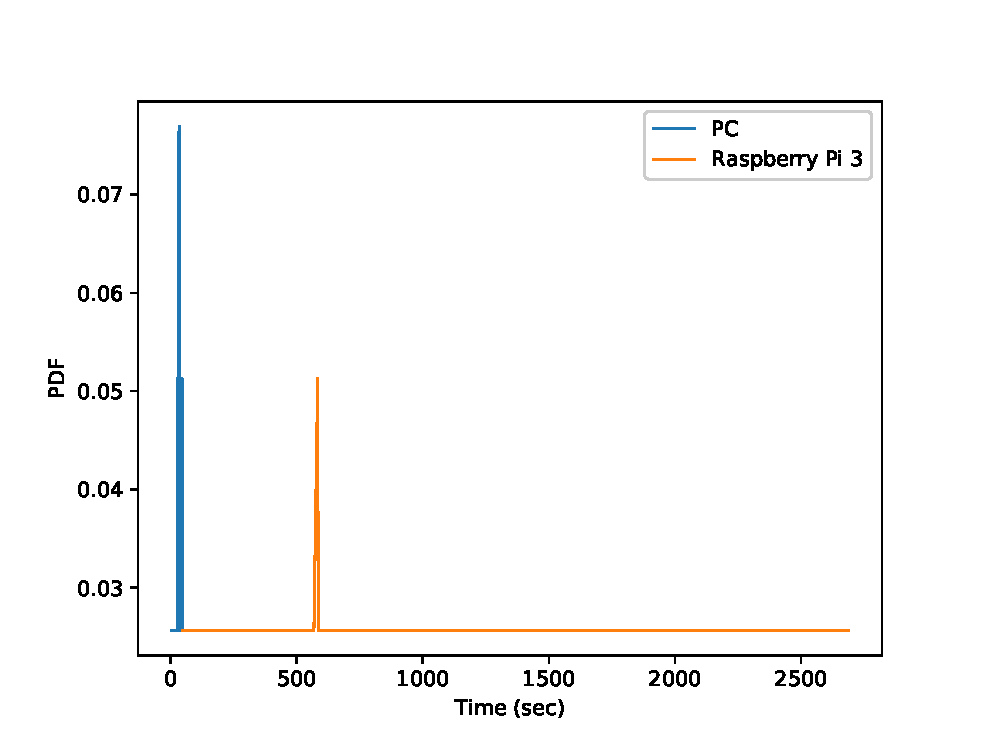
\includegraphics[width=5.in]{img/mam_send}
    \caption{The probability distributed function of time cost for sending a message through MAM.}
    \label{fig:mam_send}
\end{figure}

The simulation results above indicate that MAM is difficult for low-level sensor devices to run, whereas these kind of devices are the majority of hardware in the IoT scenarios. Furthermore, sensors with low computing power and unstable internet connection are not able to have enough resources to handle data collection, data transmission on MAM, and even trading process with subscribers simultaneously.

Therefore, transferring MAM operations to Tangle-accelerators while ensuring the profit and privacy of providers through blind signatures can effectively solve performance problems and lower the threshold to participate in such a framework. Brokers can be PCs or powerful machines that run Ethereum client and Tangle-accelerator, where Ethereum client is used to interact with Ethereum and Tangle-accelerator provides PoW acceleration and MAM delegation. Fig.~\ref{fig:rpi3_pow} shows the time cost of sending a MAM message with local Pow on Raspberry Pi 3 and remote Pow on Tangle-accelerator. However, MAM operations still cost a considerable time that improving the performance of MAM is an essential issue that needs to be done for the next step.

\begin{figure}[H]
    \centering
    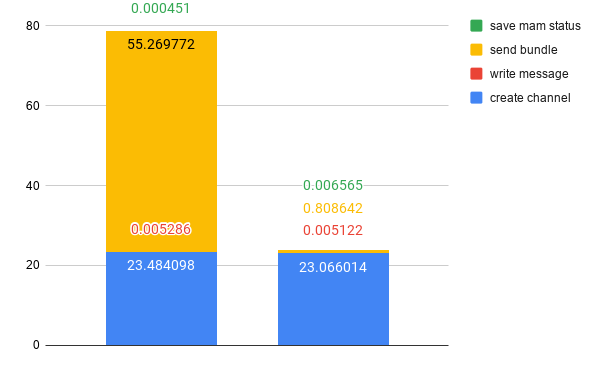
\includegraphics[width=5in]{img/rpi3_pow}
    \caption{Local PoW vs. Remote PoW}
    \label{fig:rpi3_pow}
\end{figure}

\section{MAM vs. the Delegated MAM}
\label{section:smart_contract_evaluation}

\subsection{Experiment}
Applying remote PoW greatly reduces the elapsed time. Channel creation is the next primary barrier for low-level devices to broadcast MAM message. With employing delegated MAM and E2EE, MAM channel creation would be delegated to the Tangle-accelerator which dramatically enhances the efficiency and makes MAM available for low-level devices. What follows is the performance comparison between MAM and delegated MAM (E2EE) for different payload sizes. Elapsed time for internet communication and PoW are not included, because the following processes starting from sending messages to Tangle-accelerator are the common steps. Excluding the common steps allows us to compare the performance between MAM and delegated MAM more precisely. In addition, MAM channel creation and E2EE asymmetric key pair generation are not included, too. The two excluded steps take much more time than encrypting messages only, so counting these two steps would cause extreme values. In the E2EE protocol framework, we choose SHA-256 for HMAC, AES-CBC for symmetric encryption, and Curve P-256 for ECDSA, respectively.

The steps counted in MAM benchmark including:
\begin{itemize}
    \item Encrypt the input payload
    \item Publish the last message to the Tangle network
\end{itemize}

The steps counted in E2EE benchmark including:
\begin{itemize}
    \item Generate a symmetric key for encryption
    \item Hash the input payload
    \item Encrypt the input payload
    \item Transmit the last message to the Tangle-accelerator
\end{itemize}

\begin{table}[htbp]
    \caption{Compare the performance between MAM and E2EE on Raspberry Pi 3 B+}
    \label{tab:mam_vs_e2ee}
		\centering
        \begin{tabular}{|c||c|c|}
        \hline
            \textbf{size (bytes)} & \textbf{MAM(ms)} & \textbf{E2EE(ms)} \\
            \hline
            100 & 20.28 & 9.21 \\
            500 &  26.92 & 9.27 \\
            900 & 32.02 &  9.35  \\
            1300 & 36.67 & 9.41 \\
            1700 & 40.55 & 9.54 \\
            \hline
        \end{tabular}
\end{table}

In the Table~\ref{tab:mam_vs_e2ee}, a comparison of the two results reveals the elapsing time of E2EE is obviously less than that of MAM which shows the E2EE process presented in the thesis is a much more appropriate solution for resource-constrained devices to send authenticated streaming data.

\begin{equation}
\label{eq:lin_mam}
y=0.0126 x+19.979
\end{equation}

\begin{equation}
\label{eq:lin_e2ee}
y=0.0002 x+9.174
\end{equation}

The Eq.~\ref{eq:lin_mam} and Eq.~\ref{eq:lin_e2ee} are the linear equation for the experiment data of MAM and E2EE respectively. Apparently, the slope of the result of MAM is much greater than the result of E2EE. The small slope of E2EE ensures E2EE can consistently perform in an acceptable time range.

\subsection{Time Complexity}
With the given E2EE protocol framework, ECDSA would take constant time under our situation, since the string needed to be signed is in fixed length. HMAC and AES-CBC are the procedures that cost most of the elapsed time. Time complexity of HMAC with SHA-256 is $O(n)$.\cite{hmac_time_complexity} Block cipher takes constant time for a single block which causes the time complexity is $O(n)$, too. Therefore, the E2EE protocol framework takes only linear time versus arbitrary string length. Applying mature cryptographic functions (e.g. SHA-256, AES-CBC, etc), ensures gentle slope as Eq.~\ref{eq:lin_e2ee} shows.
\clearpage

\section{Smart Contract}
In this experiment, we investigate the cost of executing Product Contract with Ethereum web browser-based IDE Remix that we can define the minimum cost, which data providers should pay in order to launch a product and processing trade.  On top of this evaluation, data providers can consider how to set the price to eventually generate profits. The estimated cost is in Ether, which is 238 USD at the time of writing, yet the price is dynamic from time to time. To conquer this condition, the authors in \cite{MindMyValue} suggested to analyze with a fixed range of Gas price,  yet the main drawback of low Gas price is the increase of time required before a transaction is validated. According to the report of Ethereum network\cite{ethereumChart} in 2020 (January to June), we set this range from 7.3 Gwei to 26.5 Gwei, which is $7.3 \times 10^{-9}$ and $2.65 \times 10^{-8}$ Ether respectively, the minimum average and average gas price. The Gas usage estimation is shown in Table.~\ref{tab:gas}.

\begin{table}[h]
	\caption{Gas consumption for each function of Product Contract}
	\label{tab:gas}
	\centering
	\resizebox{0.7\textwidth}{!}{
	\begin{tabular}{|c|c|c|c|}
		\hline
		\textbf{function} & \textbf{sender} & \textbf{Gas used} \\
		\hline
		generate contract & broker & 2558980 \\ 
		subscribe product & consumer & 72259 \\ 
		upload hashed key & provider & 68276  \\ 
		upload encryption key to consumer & provider & 86614 \\ 
		upload certified key & broker & 131535 \\
		update amount of uploaded data & broker & 32157 \\
		unsubscribe & consumer & 8234 \\
		request refund & consumer & 12067 \\
		withdraw & broker & 11313 \\
		\hline
	\end{tabular}
	}
\end{table}

Note that data uploading is only related to MAM operations on IOTA, which does not require any fees. Therefore, the Gas estimation only includes trading processes. Creating a Product Contract (Listing \ref{lst:constructor}) costs the most Gas (0.164 - 0.596 Ether), providers should have enough Ethers to launch the product at the start. Functions (Listing \ref{lst:key_exchange} (0.012 - 0.044 Ether) and Listing \ref{lst:key_certification} (0.022 - 0.0834 Ether)) that are related to key certification and key exchange need a lot of gas as well. Storage on blockchain is expensive. For instance, an SSTORE operation may cost 20000 gas when the value is set to non-zero from zero according to Ethereum Yellow Paper\cite{Ethereum}. However, in our trading model, we preserve a lot of information in the Product Contract in order to record as more details as possible during trading procedures, such as ciphertexts,  signatures during key certification and key exchange. Especially, in the key exchange protocol, it takes several steps of communications between brokers, data providers, and data consumers via storing states to Product Contract. Therefore, it is worth to explore the usage of the non-interactive zero-knowledge protocol such as zk-SNARKS(zero-knowledge succinct non-interactive argument of knowledge)\cite{Snark} which can generate proofs off-chain and simplify the verification process that could not only reduce network and storage cost but also improve the privacy and security of encryption keys. However, using the zero-knowledge protocol is out of the scope of this thesis.

Base on Gas estimation in Table.~\ref{tab:gas}, we calculate the exact Ether with Formula~\ref{equa:ether_calculation} that data providers and data consumers need during the trade in Table.~\ref{tab:ether}. We combine the Gas usage of providers and brokers since the brokerage fee is also a critical cost to sustain the trade, which providers should considered. We conclude the three situations during the trading process: 1.) basic cost of a trade, including product launching, subscribing, encryption key uploading and withdraw. 2.) refund operation, the fees needed for launching refund. 3.) unsubscribe operation, the fees needed for launching unsubscription.

\hfsetfillcolor{white!10}
\hfsetbordercolor{white}
\begin{equation}\tikzmarkin{a}(0.2,-0.5)(-0.2,0.65)
\label{equa:ether_calculation}
Ethers = Gas \ Price \times Gas \ Amount
\tikzmarkend{a}
\end{equation}

When a consumer request a refund, he/she need to pay 0.0008 - 0.0003 Ether additionally. Then if the refund established, all participants will withdraw the payment, which is already included in the basic cost. Observing the situation of unsubscribe operation, it does not cost much Ether for consumers. However, the data provider needs to update all encryption keys for remaining consumers that \textit{update encrypt key} will be triggered $N$ times, where $N$ is the number of remaining subscribers. This would cost data providers a lot if the unsubscription is frequent or many remaining consumers are left. Hence, an efficient, low-cost, and secure way to perform access control while recording the unsubscription process transparent is important. An alternative strategy coming up with the latest development of MAM, which is renaming to Streams\cite{stream}, provides new functionality for subscribers to unsubscribe to data streams, thus, it is possible to perform access control directly through it rather than uploading new encryption key to the Product Contract. Nevertheless, Streams is still in an alpha version, the details and protocol still need to be well studied.

\begin{table}[h]
    \caption{Data Price Estimation}
    \label{tab:ether}
    \centering
    \resizebox{1.\textwidth}{!}{
    \begin{tabular}{|c|c|c|c|c|c|}
        \hline
        \textbf{condition} & \textbf{sender} & \textbf{\makecell{minimum price \\ (Ether)}} & \textbf{\makecell{minimum price \\ (USD)}} & \textbf{\makecell{maximum price \\ (Ether)}} & \textbf{\makecell{maximum price \\ (USD)}} \\
        \hline
        \multirow{2}{*}{basic cost} & provider & 0.021 & 5.038 & 0.076 & 18.291 \\
         & consumer & 0.00061 & 0.145 & 0.0022 & 0.527\\
        \hhline{|=|=|=|=|=|=|}
        \multirow{2}{*}{refund} & provider & 0 & 0 & 0 & 0 \\
         & consumer & 0.00008 & 0.0209 & 0.0003 & 0.0761 \\
        \hline
        \multirow{2}{*}{unsubscribe} & provider & 0.002N & 0.497N & 0.007N & 1.806N \\
         & consumer & 0.00006 & 0.0143 & 0.0002 & 0.0519 \\
        \hline
    \end{tabular}
    }
\end{table}

\end{spacing}

\clearpage
\setstretch{1.2}

% ------------------------------------------------
%                   Conclusion
% ------------------------------------------------
\newpage
\phantomsection
\chapter{Conclusion}
\label{section:conclusion}
\pagestyle{plain}

\begin{spacing}{2.0}

By combining the established standards and openly-developed specifications, this thesis proposed a highly decentralized, autonomous publish/subscribe model design that combines data storage and trading together in order to ensure the digital rights of both data providers and consumers during the dynamic data streaming trading. It was built with blockchain network, immutable audit trails, and contracts with an integrated decentralized identity system, to enable the data stream trading by shifting risks from centralized services, ensure the authenticity of all participants, clarify the data ownership, enable secure communication and flexible trading mechanisms.

Compared to previous works, we 1.) identify a trustless data trading infrastructure, 2.) ensure the confidentiality of scalable IoT-based sensor data, and 3.) consolidate the economic incentives in the entire ecosystem. Meanwhile, we consider the heavy workload of the low-level sensors, conduct an experiment which authenticates the data providers to delegate the MAM operations to Tangle-accelerators, and conclude that the performance of the E2EE approach is more fitting than the MAM solution. In particular, this work discusses the workflow for subscription-based IoT data trading: Launching, subscribing, unsubscribing, and refund.

\end{spacing}

\clearpage
\setstretch{1.2}

% ------------------------------------------------
%                   Future Work
% ------------------------------------------------
\newpage
\phantomsection
\chapter{Future Work}
\label{section:future_work}
\pagestyle{plain}

\begin{spacing}{2.0}

In the subscription-based data trading, there are some issues worth discussing and improving. Firstly, reduce the Gas usage of trading models, as we mentioned in Section~\ref{section:smart_contract_evaluation}, the key exchange process consumes a lot of Gas due to the frequent store operation. Therefore, it is worth discussing how zero-knowledge protocol could used to exchange the key with lower cost, and even validate the key within transfers. Second, brokers are the key to operating a stable system, since they are irreplaceable either from the view of architecture design or trading procedures. However, issues such as the minimum number of brokers needed to operate the system, and the evaluation of adopting gossip protocol among brokers to gossipped trading status, which enables other brokers to handle trading processes when on crashed.

Third, to let consumers search and find interesting data products, a search engine is needed to collect all distributed data products, which might need the authority to design and run the service. The extending issue of searching is ranking, how would the search service provider rank the products, how would that affect data consumers and providers. Fourth, in our design, we do not restrict the qualifications of data providers and brokers, which is different from operating the App store currently, and it is also an interesting issue to discuss.


\end{spacing}

\clearpage
\setstretch{1.2}

% ------------------------------------------------
%               參考文獻 References
% ------------------------------------------------
% References and bibliography

% Import the files that contain your references.
% If you set some references file,
% you need to use at least one cite to make Latex work.
\singlespacing
\newpage
\phantomsection
\renewcommand\bibname{References}	% references title

% 學校規定以作者英文姓氏第一字排列順序,故使用 plain ,如果要按照引用順序,可改用 ieeetr
\bibliographystyle{plain}			% reference style
\bibliography{thesis}				% target .bib file

\clearpage
\setstretch{1.2}

\end{document}